%#!platex
\documentclass[11pt,a4j]{jbook}

\title{$B=$;NO@J8(B \\
  \vspace{1cm}
  {\Huge $B89M}O@$NHs2D494v2?3XE*B&LL(B}\\
  \vspace{7cm}}
\author{ $B;T@n(B \hspace{3mm}$B7{?M(B
   \footnote{kent@hep-th.phys.s.u-tokyo.ac.jp}
   ($B3X@RHV9f(B96036)\\
   \large $BEl5~Bg3XM}3X7O8&5f2JAGN3;RM}O@8&5f<<(B
   \vspace{-2mm} \\
   \large $BEl5~ETJ85~6hK\6?(B 7-3-1 \\
   \vspace{2cm}}
\date{}

%#!platex master.tex
% Packages used
\usepackage{graphicx}
\usepackage{color}
\usepackage{amsmath}
\usepackage{amssymb}
\usepackage{amsfonts}
\usepackage{amsthm}
\usepackage{amsxtra}
\usepackage{mathrsfs}
\usepackage[all]{xypic}
\usepackage{enumerate}

% \CompileMatrices
% Define theorem environment
\newtheoremstyle{mythmsty}{3pt}{3pt}{\upshape}{}{\upshape\bfseries}{}{\newline}{}
\theoremstyle{mythmsty}
\renewcommand{\proofname}{{\bfseries $B>ZL@(B}}
\newtheorem{The}{$BDjM}(B}[section]
\newtheorem{Def}[The]{$BDj5A(B}
\newtheorem{Lem}[The]{$BJdBj(B}
\newtheorem{Cor}[The]{$B7O(B}
\newtheorem{Conj}[The]{$B2>@b(B}

%make upshape default
\upshape

% Some outlooks
\setlength{\textwidth}{150mm}
% for jbook
\renewcommand{\bibname}{$B;29MJ88%(B}
\setlength{\evensidemargin}{-3mm}
\setlength{\oddsidemargin}{7mm}
% for jreport
%\setlength{\evensidemargin}{5mm}
%\setlength{\oddsidemargin}{5mm}

%Some abbreviations
\def\sla#1{\rlap{\kern .15em /}#1}
\def\bra#1{\langle #1 |}
\def\ket#1{| #1 \rangle}
\def\ten{\textperiodcentered}
\def\der{\partial}
\def\1half{\frac{1}{2}}
\def\ihalf{\frac{i}{2}}
\def\kbar{{\mathchar'26\mkern-9muk}}

\def\vl{\vec{l}}
\def\vk{\vec{k}}
\def\vp{\vec{p}}
\def\ap{{\alpha'}}
\def\ls{{\ell_{\mathrm{s}}}}
\def\Ud{U^\dagger{}}

\def\rht{{\tilde{\rho}}}
\def\Kt{{\tilde{K}}}
\def\Ab{{\bar{A}}}
\def\At{{\tilde{A}}}
\def\Ah{{\hat{A}}}
\def\Dh{{\hat{D}}}
\def\Dt{{\tilde{D}}}
\def\Fh{{\tilde{F}}}
\def\Ft{{\tilde{F}}}
\def\xh{{\hat{x}}}
\def\yh{{\hat{y}}}
\def\zb{{\bar{z}}}
\def\derb{{\bar{\partial}}}
\def\delh{{\hat{\delta}}}
\def\delt{{\tilde{\delta}}}
\def\lamh{{\hat{\lambda}}}
\def\lamt{{\tilde{\lambda}}}
\def\theh{{\hat{\theta}}}
\def\thet{{\tilde{\theta}}}

\def\Cst{\mathrm{C}^*{}}
\def\Cinf{\mathrm{C}^\infty}

\def\crea{a^\dagger{}}
\def\anih{a}
\def\creC{{C^*}}
\def\aniC{{C}}
\def\Sd{{S^*}}
\def\Tb{{T^*}}


\def\zero{\mathbf{0}}
\def\E{\mathrm{e}}

\def\Ad{\mathrm{Ad}}
\def\Aut{\mathrm{Aut}}
\def\Arg{\mathrm{Arg}}
\def\CoD{\mathrm{cod}\,}
\def\Diag{\mathrm{diag}}
\def\Dim{\mathrm{dim}}
\def\Dom{\mathrm{dom}\,}
\def\End{\mathrm{End}}
\def\Ext{\mathrm{\mathbf{Ext}}}
\def\GL{\mathrm{GL}}
\def\Ham{\mathrm{H}}
\def\Hom{\mathrm{Hom}}
\def\Ker{\mathrm{Ker}}
\def\id{\mathrm{id}}
\def\Img{\mathrm{Im}}
\def\Ind{\mathrm{Index}}
\def\n{\mathrm{n}}
\def\Ob{\mathrm{Ob}}
\def\Rank{\mathrm{Rank}}
\def\Tr{\mathrm{Tr}}
\def\Vect{\mathrm{Vect}}


\def\bx{\mathbf{x}}
\def\AlgA{\mathcal{A}}
\def\AlgAk{{\mathcal{A}_\kbar}}
\def\AlgB{\mathcal{B}}
\def\AlgC{\mathcal{C}}
\def\AlgJ{\mathcal{J}}
\def\AlgK{\mathcal{K}}
\def\CatA{\mathscr{A}}
\def\CatB{\mathscr{B}}
\def\CatC{\mathscr{C}}
\def\ModM{\mathcal{M}}
\def\ModN{\mathcal{N}}
\def\ModE{\mathcal{E}}
\def\ModF{\mathcal{F}}
\def\Mat{\mathrm{Mat}}
\def\MatK{\mathbb{K}}
\def\Mtrx{\mathbb{M}}
\def\Minf{{\mathbb{M}_\infty}}
\def\OpO{\mathcal{O}}
\def\Toep{\mathcal{T}}
\def\Spi{\mathcal{S}}

\def\Real{\mathbb{R}}
\def\Cplx{\mathbb{C}}
\def\Rtnl{\mathbb{Q}}
\def\Hil{\mathscr{H}}
\def\Intg{\mathbb{Z}}
\def\Ntrl{\mathbb{N}}
\def\Ord{\mathcal{O}}
\def\Trvn{\mathfrak{n}}
\def\Trvm{\mathfrak{m}}


\def\AntiSymBlock#1{
\begin{matrix}
 0   & #1 \\
 -#1 & 0  \\
\end{matrix}}

\begin{document}

\maketitle

\tableofcontents
%%
%% Introduction
%%
\chapter{Introduction}
\label{introduction}
%#!platex master.tex
\section{$B=x(B}
$BJ*M}3X$H$O!"2f!9$N7P83$NCf$+$iDjNLE*$JItJ,$rCj=P$7$F!"$=$N0l8+IT5,B'$J7P(B
$B83$NMeNs$NCf$+$i?t3X$N8@MU$G5,B'@-$r8+$$=P$=$&$H$$$&;n$_$G$"$k!#$3$N;n$_(B
$B$,Bg$$$K@.8y$7!"2f!9$,7P83$9$k8=>]$NA4$F$N4pAC$KJ*M}3X$,$"$k$H?.$8$i$l$k(B
$B$h$&$K$^$G$J$C$?;v$O!"Bg$-$J6C$-$G$"$k!#99$K!"2f!9$,IaCJ?($l$F$$$k%9%1!<(B
$B%k$H$O0[$J$k%9%1!<%k$K1w$$$F$O!"NL;RO@$dAjBPO@$N$h$&$K2f!9$ND>4Q$H0[$J$k!"(B
$B?t3XE*$JIAA|$,$h$jK\<AE*$G$"$k$3$H$,J,$+$k$3$H$,$7$P$7$P$"$C$?!#$3$&$7$?(B
$B7P83E*;v<B$O!"2f!9$,7P83$9$k;vJ*$NK\<A$,?t3XE*$J$b$N$G$"$k$3$H$rM=46$5$;(B
$B$k$b$N$G$"$k!#(B

$BJ*M}3X$NBg$-$JL\I8$N0l$D$O!"E}0lM}O@B($A!"MM!9$J%9%1!<%k$G2f!9$N7P83$7F@(B
$B$kA4$F$N;v$r!">/$J$/$H$b86M}E*$K$O@bL@$9$k$3$H$N$G$-$kBN7O$rC[$->e$2$k$3(B
$B$H$G$"$k!#$=$N:n6H$,!"2f!9$,7P83$K$h$C$FF@$?D>46E*$JIAA|$K?t3X$N8@MU$rEv(B
$B$F$O$a$k$3$H$G@.$7?k$2$k$3$H$,$G$-$l$P!"$=$l$K1[$7$?$3$H$O$J$$!#$7$+$7!"(B
$BJ*M}3X$NL\;X$9BN7O$O!"2f!9$,7P83$K$h$C$FF@$?@$3&$NIAA|$H$O0[$J$k@$3&$NIA(B
$BA|$rI,MW$H$9$k$b$N$G$"$k$+$bCN$l$J$$!#$=$N$h$&$J;v$,J*M}$K$*$$$F$O2a5n$K(B
$B2?EY$+$"$C$?!#$b$72f!9$ND>4QE*$J@$3&$NIAA|$,@53N$J$b$N$G$O$J$+$C$?$jK\<A(B
$BE*$G$J$+$C$?$j$7$?$H$9$l$P!"@5$7$$IAA|$r5-=R$9$k$3$H$N$G$-$kJL$N8@8l$,I,(B
$BMW$G$"$k!#$=$N$h$&$J8@8l$O!"21$i$/=c?h$K?t3X$N8@8l$G$"$k$H9M$($i$l$F$-$?(B
$B8@8l$G$"$k!#(B

$B6aG/$h$/8@$o$l$k$3$H$@$,!"8=:_$NJ*M}3X$N>u67$ONL;RNO3X$NCB@8D>A0$N>u67$H(B
$B$h$/;w$F$$$k$H;W$o$l$k!#NL;RNO3X$K1w$1$kNL;R2=$H$OB($A!VBe?t$N8@MU$KD>$7(B
$B$F0l@#!"$:$i$7$F9M$($F$_$k!W$H$$$&$3$H$G$"$k!#$3$NO@J8$G@bL@$9$kHs2D494v(B
$B2?3X$N<B8=J}K!$N$R$H$D$G$"$kJQ7ANL;R2=$H$O!"$^$5$K$=$N!V0l@#!"$:$i$9!W$H(B
$B$$$&0UL#$G$NNL;R2=$G$"$k!#$3$3$KN`;w@-$r8+=P$9$3$H$,$G$-$k!#L5O@$3$l$O@5(B
$B3N$J5DO@$G$O$J$$!#$7$+$7$R$H$D$N9M$(J}$H$7$F!"<!$N$h$&$J$3$H$r9M$($k$3$H(B
$B$,$G$-$k!#2f!9$,7P83$7$F$$$k;v>]$N!"6u4V$dJ*<A$H$$$C$?EAE}E*$J!V2J3XE*<B(B
$B:_!W$K$h$k5-=R$N;EJ}$O2f!9$N%9%1!<%k$G5/$-$F$$$k;v>]$r5-=R$9$k$N$KJXMx$G(B
$B$"$k$+$i!"2f!9$,7P83E*$K3MF@$7$?5-=RK!$G$"$k!#$7$+$7!"2f!9$N%9%1!<%k$+$i(B
$BN%$l$?%9%1!<%k$N;v>]$r5-=R$7$h$&$H$9$l$P!"$=$N5-=R$N;EJ}$r!V$:$i$9!WI,MW(B
$B$,$"$k!#>l$NNL;RO@$NOH$rD6$($F(BPlanck $B%9%1!<%k$N;v>]$^$G5-=R$9$kBN7O$rF@(B
$B$h$&$H$7$?;~$K$O!"NL;R2=$K$h$C$F!V$:$i$7$?!W@$3&$NIAA|$r$5$i$K!V$:$i$9!W(B
$BI,MW$,$"$k$+$bCN$l$J$$!#$=$N!V$:$i$7!WJ}$OJQ7ANL;R2=$NOHAH$NCf$K<}$^$k$H(B
$B$O8B$i$J$$$,!"Hs2D494v2?3X$O2D49$J6u4V$NJQ7ANL;R2=$rD6$($?BP>]$r07$$F@$k(B
$BBN7O$G$"$j!"I,MW$H$5$l$k!V$:$i$7!WJ}$OHs2D494v2?3X$NOHAH$KF~$C$F$$$k$3$H(B
$B$,4|BT$G$-$k!#(B

$B$3$3$^$G$N5DO@$O!"Hs2D494v2?3X$r8&5f$9$k$3$H$,K\Ev$KI,MW$J$N$+$H$$$&Ld$$(B
$B$KBP$9$kEz$($K$O$J$C$F$$$J$$!#6u4V$NJQ7ANL;R2=$d$=$NB>$N!V$:$i$7!WJ}$G6u(B
$B4V$NIAA|$r$:$i$9$3$H$,I,MW$G$"$k$+$I$&$+$b$^$?J,$+$i$J$$!#$?$@!"E}0lM}O@(B
$B$r40@.$9$k$NHs2D494v2?3X$N8@MU$,I,MW$G$"$k$+$bCN$l$J$$$H$$$&$3$H$r8@$C$F(B
$B$$$k$K2a$.$J$$!#2f!9$NJ*M}$r5-=R$9$kJ}K!$,Hs2D494v2?3X$r4^$^$M$P$J$i$J$$(B
$B$H$$$&M}M3$O!"FC$K$OCN$i$l$F$$$J$$!#$7$+$7!"$=$l$r<(:6$9$k$h$&$JK5>Z$O$$(B
$B$/$D$,B8:_$9$k!#$3$NO@J8$G$O$=$&$7$?K5>Z$r$$$/$D$+>R2p$7$F$$$-$?$$!#(B

$B:G8e$K!"0J>e$O8D?ME*$K9M$($?A4$/JP8+$KK~$A$?J*$N8+J}$G$"$j!"$"$/$^$G$b0l(B
$B3X@8$N9M$($?$R$H$D$NJ*$N8+J}$K2a$.$J$$$3$H$r=E$M$F6/D4$7$F$*$/!#(B

\section{$BHs2D494v2?$H89M}O@(B}
$B89M}O@$O!"=ENO$r4^$`E}0lM}O@$H$7$F:G$bM-NO$J8uJd$G$"$k!#>/$J$/$H$b!"E,Ev(B
$B$J??6u$r<j$GA*$Y$P!"$H$j$"$($:$O=ENO$HI8=`LO7?$NE}0lM}O@$r:n$k$3$H$,$G$-(B
$B$k!#$7$+$7!"$=$NHs@]F0O@E*$JDj<02=$OL$$@40@.$5$l$F$$$J$$!#=>$C$F!"$I$N$h(B
$B$&$J??6u$,A*$P$l$k$N$+$H$$$&%a%+%K%:%`$OJ,$+$C$F$$$J$$!#8=>u$G$O!"89M}O@(B
$B$NHs@]F0O@E*$JDj<02=$rL\;X$7$F!"APBP@-$J$I$N<jK!$rMQ$$$FHs@]F0O@E*$JDj<0(B
$B2=$K8~$1$?@9$s$J8&5f$,$J$5$l$F$$$k!#(B

$B0lJ}!"Hs2D494v2?3X$O!"<g$K?t3X<T$N(BConnes$B$i$K$h$C$F8&5f$N?J$a$i$l$F$$$k4v(B
$B2?3X(B\footnote{$BHs2D494v2?3X$N85$N%"%$%G%#%"$O(Bvon Neumann$B$^$G$5$+$N$\$k!#(B}
$B$G!"<g$KJ*M}$H$O0[$J$k%b%A%Y!<%7%g%s$G8&5f$5$l$F$-$?!#Hs2D494v2?3X$O0lHL(B
$B$K8@$o$l$k$H$3$m$N2D49$J4v2?3X$r4^$`$h$jBg$-$JCj>]E*$J4v2?3X$NOHAH$G$"$k!#(B
$BHs2D494v2?3X$N9M$(J}$N=EMW$JE@$O!"B?MMBN$=$N$b$N$h$j$b$=$N>e$N4X?t$N@.$9(B
$B4D$r$h$jK\<AE*$J$b$N$H8+$J$9E@$K$"$k!#$=$3$G$O!"0lHL$K$O:BI8$dE@$N35G0$b(B
$B<+L@$J$b$N$G$O$J$/!"2f!9$N4v2?$KBP$9$kD>4Q$+$i$+$J$jN%$l$?BP>]$r$b07$$F@(B
$B$kBN7O$G$"$k!#(B

$BHs2D494v2?3X$N0J>e$N$h$&$J@-<A$r4*0F$9$k$H!"Hs2D494v2?3X$O8=<BE*$JBP>]$r(B
$B07$&J*M}$H$O0l8+2?$N4X78$bL5$$$h$&$K;W$($k$,!"Hs2D494v2?$N4pK\E*$J9M$(J}(B
$B$G$"$kB?MMBN$N>e$N4X?t$N@.$94D$rK\<A$H9M$($k;v<+BN$O!"AGN3;RJ*M}3X$H$N?F(B
$BOB@-$,9b$$!#2?8N$J$i!"2f!9$,=;$s$G$$$k;~6u$N4v2?3X$rCN$m$&$H;W$C$?;~!"2f!9(B
$B$O$=$N>e$K$"$k>lB($AB?MMBN$N>e$N4X?t$K$h$C$F$7$+;~6u$K$D$$$F$N>pJs$rF@$k(B
$B$3$H$,$G$-$J$$$+$i$G$"$k!#$=$N0UL#$G!"J*M}3X$NK\<A$r9M$($k>e$G!";~6u$N4v(B
$B2?3X$r5-=R$9$k$d$jJ}$NA*Br;h$N$R$H$D$H$7$FHs2D494v2?3X$r9M$($k$N$O<+A3$J(B
$B9M$($G$"$k$H$$$($k!#(B

$B99$K!"<B:]E*$JHs2D494v2?3X$N9=@.K!$G$"$k$H;W$o$l$kJQ7ANL;R2=$NJ}K!$OM}O@(B
$B$K0?$k:G>.$N%9%1!<%k$rM?$($k$H$$$&E@$G!"J*M}3X$NBgL\I8$N$R$H$D$G$"$kNL;R(B
$B=ENOM}O@$N9=@.$K7hDjE*$J2r7h:v$rM?$($k$H$$$&4|BT$r;}$?$;$k!#89M}O@$,NL;R(B
$B=ENOM}O@$H$7$F>e<j$/$$$C$F$$$kM}M3$b$^$?!"89M}O@$,Hs2D494v2?3XE*$JB&LL$r(B
$B;}$C$F$$$k$+$i$G$"$k$H9M$($k$3$H$,$G$-$k!#(B

$B<B:]!"89M}O@$K1w$$$F$O(B
\begin{itemize}
 \item $B89M}O@$K$O(B $B;~6u$NIT3NDj@-$,$"$k$3$H(B\cite{STandS-TUnCertainty}$B!"(B
 \item $B;~6u(B $B$N:BI8$rHs2D49$J9TNs$HB*$($k9TNsLO7?$,89M}O@$NHs@]F0O@E*$JDj<0(B
       $B2=$K$J$C$F$$$k$i$7$$$3$H(B\cite{IKKTMatrix}\cite{BFSSMatrix}
 \item String Field Theory$B$H$N4X78$,$"$k$3$H(B\cite{NCGandSFT}$B!"(B
 \item $BFCDj$N6K8B$N$b$H$G89M}O@$+$i;~6u$NHs2D49@-$,<+A3$K8=$o$l$k$3$H(B
       \cite{YMforNCT2}$B!"(B
\end{itemize}
$B$J$I$N;v<B$,!"(B80$BG/BeH>$P$+$i;XE&$5$l$F$$$?!#(B

$B:G6a$K$J$C$F!"%H!<%i%9>e$N9TNsLO7?$,Hs2D49%H!<%i%9$r<+A3$K4^$`$3$H$d!"(B
Seiberg-Witten$B<LA|$d(BGMS$B%=%j%H%s$NH/8+$dHs2D49%b%N%]!<%k$K$D$$$F$N8&5f$N?J(B
$BE8$G!"Hs2D494v2?$H89M}O@$N7k$SIU$-$O$h$j6/8G$J$b$N$H$J$j!"@9$s$K8&5f$5$l$k(B
$B$h$&$K$J$C$?!#Hs2D494v2?3X$O!"89M}O@$rE}0lM}O@$H$7$FM-NO$JM}O@$?$i$7$a$kMW(B
$B7o$G$"$k$H9M$($i$l$k$H$$$&0UL#$G!"89M}O@$NHs@]F0O@E*$JDj<02=$rF@$k0Y$N=EMW(B
$B$JF;6q$G$"$jF@$k!#(B

$B89M}O@$OM}O@$N%Q%i%a!<%?$r(B$\ap$$B$R$H$D$7$+;}$?$:!"<B$KMM!9$JM}O@$,89M}O@(B
$B$N$"$k??6u$NA*$SJ}$K$h$C$F<B8=$G$-$k$H$$$&0UL#$G!"Hs>o$K6/NO$JIaJW@-$r;}$C(B
$B$F$$$k!#$b$789M}O@$NHs@]F0O@E*$JDj<02=$r40@.$9$k$3$H$,$G$-!"$+$D!"@$3&$N(B
$BHs2D494v2?3XE*$JIAA|$,E}0lM}O@$r5-=R$9$k$N$KI,MW$G$"$k$H$9$k$J$i$P!"89M}(B
$BO@$NHs@]F0O@E*$JDj<02=$OHs2D494v2?3X$rI,$:4^$s$G$$$kH&$G$"$k!#$^$?!"89M}(B
$BO@$NHs@]F0O@E*$JDj<02=$rC5$k>e$GHs2D494v2?3X$OBg$-$J%R%s%H$rM?$($F$/$l$k(B
$B$H4|BT$G$-$k!#(B

\section{$BFbMF35@b(B}
$B$3$NO@J8$G$O!"$^$:Bh(B\ref{mathmatics}$B>O$GHs2D494v2?3X$N?t3XE*9=@.$K$D$$$F=R(B
$B$Y$k!#$3$3$G$O!"(BConnes$BN.$NCj>]E*$JHs2D494v2?$NDj5A$H!"JQ7ANL;R2=$K$h$k$h(B
$B$j8=<BE*$JHs2D494v2?$N9=@.K!$K$D$$$F=R$Y$k!#99$K!"Hs2D494v2?$K$*$1$kHyJ,4v(B
$B2?$NDj5A$H$=$l$K$h$k@\B3$N35G0$r>R2p$9$k!#(B

$BBh(B\ref{application}$B>O$G$O$^$:!"DL>o$N>l$NM}O@$KHs2D49@-$rF3F~$9$kF05!$K(B
$B$D$$$F@bL@$9$k!#$3$3$G$O!"Dc%(%M%k%.!<M-8zM}O@$H$7$FI8=`LO7?$r4^$`$h$&$J(B
$BM}O@$NCf$G$O!"Hs2D494v2?E*$J@-<A$r;}$C$?M}O@$,=ENO$HI8=`LO7?$NE}0lM}O@$H(B
$B$7$FM-NO$G$"$k$3$H$,<(:6$5$l$k!#<!$K!"Hs2D494v2?$r>l$NM}O@$K1~MQ$9$kJ}K!(B
$B$H!":G$b4JC1$KHs2D49@-$rF3F~$7$?>l$NM}O@$N@]F0O@5Z$S$=$N7+$j9~$_$K$D$$$F(B
$B@bL@$9$k!#:G8e$KHs2D49>l$NM}O@$K$D$$$FCN$i$l$F$$$k!"Hs2D49@-$KM3Mh$9$kHs(B
$B2D49>l$NM}O@$KFHFC$J=t@-<A$r$$$/$D$+>R2p$9$k!#(B

$BBh(B\ref{emergence}$B>O$G$O89M}O@$,K\<AE*$KHs2D494v2?$G$"$k>Z5r$H$J$C$F$$$k(B
$B$H;W$o$l$k;~6u$NIT3NDj@-$K$D$$$F@bL@$9$k!#<!$K!"Hs@]F0O@E*$JDj<02=$G$"$k(B
$B$H9M$($i$l$F$$$k(BString Field Theory$B$N:nMQ$K8=$o$l$k(B$*$$B@Q$K$D$$$F@bL@$7!"(B
$B$=$NHs2D494v2?3X$H$N4X78$K$D$$$F5DO@$9$k!#99$K!"89M}O@$NFCDj$N@_Dj$N2<$G(B
$B$ODc%(%M%k%.!<M-8zM}O@$,Bh(B\ref{application}$B>O$G>R2p$7$?Hs2D49%2!<%8>lM}(B
$BO@$G$"$k$3$H$r@bL@$7!"(BSeiberg-Witten$B<LA|$,89M}O@$G$N%l%.%e%i%j%<!<%7%g%s(B
$B$N0c$$$H$7$F<+A3$K2r<a$9$k$3$H$,$G$-$k$3$H$r@bL@$9$k!#$^$?!":G6a=EMW$J8&(B
$B5fBP>]$K$J$C$F$$$k(BGMS$B%=%j%H%s$K$D$$$F@bL@$7$=$N(BD-brane$B$H$N4X78$r(BK-theory 
$B$N8@MU$rMQ$$$F@bL@$9$k!#:G8e$K!"(BD-brane$B$H(B$K$-theory$B$N4X78$r4v$D$+$NJ}K!(B
$B$rMQ$$$F=R$Y$k!#(B

$BBh(B\ref{conclusion}$B>O$G$O0J>e$N>O$G@bL@$7$?;v$N4JC1$J$^$H$a$H:#8e$N89M}O@(B
$B$NHs2D494v2?3XE*B&LL$K$D$$$F$N8&5f$NE8K>$r=R$Y$k!#(B

$B$^$?!"(BAppendix$B$G$O7w$N35G0$H4v2?E*$J(B$K$-thoery$B$H(B$\Cst$$B4D$N(B$K$-theory$B$N4JC1(B
$B$J>R2p$r$9$k!#(B

\section{$B%3%s%Y%s%7%g%s(B}
\label{convention}

\begin{itemize}
 \item $B89M}O@$N(B$B_{\mu\nu}$$B>l$O(B$g_{\mu\nu}$$B$HF1$8<!85$r;}$C$?Dj5A$H!"EE(B
       $B<'>l(B$F_{\mu\nu}$$B$HF1$8<!85$r;}$C$F$$$kDj5A$N(B2$BDL$j$,$"$k$,!"$3$3$G(B
       $B$O8e<T$NJ}$NDj5A$r:NMQ$9$k!#B($A$=$N%P!<%F%C%/%9%*%Z%l!<%?$O(B
       ${1\over 2\pi\ap}B_{\mu\nu}\partial X^\mu\partial Y^\nu$$B$G$"$k!#(B
 \item \begin{minipage}[t]{13mm}
	$BDj?t(B\\
	\begin{tabular}{rl}
	 Planck$BDj?t(B\ten $B8wB.(B & $\hbar=c=1$ \\
	 $B89$N%F%s%7%g%s(B & $\ap$ \\
	 $B89$N%9%1!<%k(B & $\ls =\sqrt{\ap}$
	\end{tabular}
       \end{minipage}
 \item \begin{minipage}[t]{130mm}
       	$B5-9f(B(*$B$,$D$$$F$$$k$b$N$O2<$GDj5A$9$k!#(B)\\
      	\begin{tabular}{rl}
	 Worldsheet$B$N:BI8(B($B6u4VJ}8~!";~4VJ}8~(B) 
	 & $\sigma=\sigma_1,\tau=\sigma_2$ \\
	 $B;~4V$r4^$`:BI8$NE:;z(B & $\mu,\nu,\ldots$ \\
	 $B;~4V$r4^$^$J$$:BI8$NE:;z(B & $i,j,\ldots$ \\
	 $B7w(B & $\CatA,\CatB,\CatC,\ldots$ \\
	 $BBe?t!"H>72(B & $\AlgA,\AlgB,\ldots$ \\
	 $\AlgA$$B2C72(B(module)$B$?$@$7!"(B$\AlgA$$B$OBe?t(B* 
	 & $\ModE,\ModM,\ModN,\ldots$ \\
	 $B6u4V(B & $X,Y,\ldots$ \\
	 $B<+A3?t(B,$B@0?t(B,$B<B?t(B,$B@5?t(B,$BJ#AG?t(B &
	 $\Ntrl,\Intg,\Real,\Real^+,\Cplx$ \\
	 $\AlgA$$B78?t$N7A<0E*f25i?t4D(B & $\AlgA[[x]]$ \\
	 $\AlgA$$B78?t$N(B$n\times n$$B9TNs4D(B & $\Mtrx_n(\AlgA)$ \\
	 $\Mtrx_n$$B$N5"G<E*6K8B(B* & $\Minf$ \\
	 $\Minf$$B$NCf$N%3%s%Q%/%H$J85$N=89g(B& $\MatK$ \\
	 $B>hK!C10L85$r;}$D(B$\AlgA$$B78?t$N2D5U$J(B$n\times n$$B9TNs(B
	 & $\GL_n(\AlgA)$ \\
	 $B>hK!C10L85$r;}$D(B$\AlgA$$B78?t$N(B$n\times n$$B%f%K%?%j9TNs(B
	 & $U_n(\AlgA)$ \\
	 $B6u=89g(B & $\phi$ \\
	 $BDj5A(B & $A\equiv B$ \\
	 $BF17?(B & $\AlgA\cong\AlgB$ \\
	 $B0LAjF1Aj(B & $X \approx Y$ \\
	 $B<LA|(B$f$$B$N(B$X$$B$X$N@)8B(B & $f\mid X$ \\
	 $B9g@.<LA|(B & $f\circ g$ \\
	 $B>&72(B($BIaDL$N3d$j;;$r4^$`(B) & $M\diagup N$ \\
	 1$BE@%3%s%Q%/%H2=(B* & $X^\infty$ \\
	 $BEy2=6u4V(B & $X/Y$ \\
	 Moyal$B@Q(B & $\phi\star\psi(x)\equiv
	 \E^{\ihalf\theta^{\mu\nu\partial^y_\mu\partial^z_\nu}}
	 f(y)f(z)\Big|_{x=y=z}$ \\
	 Moyal$B@Q$K$h$k8r49;R(B & $[A,B]_\star\equiv A\star B-B\star A$
       	\end{tabular}
       \end{minipage} 
       \begin{Def}[$B:8(B$\AlgA$$B2C72(B(module)]
	$BBe?t(B$\AlgA$$B$N:nMQ$N$"$k72(B$\ModM$$B$H$O!"(B$a,b\in\AlgA\, ,\beta
	,\alpha\in\ModM$$B$G!"<!$N@-<A$rK~$?$9$b$N$r$$$&!#(B
	\begin{enumerate}[M1]
	 \item $(\alpha + \beta)a=\alpha a+\beta a$
	 \item $(\alpha\beta)a=\alpha(\beta a)$
	 \item $\alpha(a+b)=\alpha a + \alpha b$
	\end{enumerate}
       \end{Def}
       \begin{Def}[1$BE@%3%s%Q%/%H2=(B]
	$B0LAj6u4V(B$X$$B$N(B1$BE@%3%s%Q%/%H2=$H$O!"(B$X$$B$N30It$NE@(B$\{\infty\}$$B$r(B$X$
	$B$K2C$($?$b$N$G$"$k!#B($A(B$X\cup\{\infty\}$$B!#99$K!"(B$X$$B$N$b$H$b$H$N(B
	$B3+=89gB2$K3+=89g$H$7$F(B$Y$$B$rG$0U$N(B$X$$B$NItJ,%3%s%Q%/%H6u4V$H$7$F!"(B
	$\{(X-Y)\cup\{\infty\}\}$$B$r2C$($?$b$N$G$"$k!#(B\\$BD>46E*$K$O%3%s%Q(B
	$B%/%H$G$J$$=89g$NC<$r(B1$BE@$K=8$a$F$=$3$K(B1$BE@$r2C$($?$b$N$G$"$k!#(B
       \end{Def}
       \begin{Def}[$n\times n$$B9TNs4D$N(B$n\rightarrow\infty$$B5"G<E*6K8B(B$\Minf$]
	\label{infinite-matrix}
	$\Mtrx_n$$B$N5"G<E*6K8B(B$\Minf$$B$O(B$n\times n$$B9TNs4D(B$\Mtrx_n$$B$NNs$N6K(B
	$B8B$G!#Jq4^<LA|$H$7$F(B$\Phi_{mn}:\Mtrx_m\rightarrow\Mtrx_n 
	\,(m<n)$$B$O(B$n\times n$$B9TNs$N:8>e$K(B$m\times m$$B9TNs$rKd$a9~$`$h$&$J(B
	$B<LA|$K$D$$$FM#0l$DDj5A$G$-$k$h$&$J$b$N$G$"$k!#D>46E*$K$O!"(B
	$\infty\times\infty$$B9TNs$G3F(B$n\times n$$B9TNs$N4D$,:8>e$KKd$a9~$^(B
	$B$l$F$$$k$h$&$J4D$G$"$k!#>\:Y$O!"(B\cite[AppendixL]{Wegge-OlsenKth}
	$B$r;2>H!#(B
       \end{Def}
       \begin{Def}[$B%3%s%Q%/%H:nMQAG$N$J$94D(B$\MatK$]
	$BDj5A(B\ref{compact-operator}$B$r;2>H!#(B
       \end{Def}
\item Fourier$BJQ49(B
       \begin{equation}
	\tilde{f}(k)\equiv{1\over (2\pi)^{d/2}}
	 \int d^dx\,f(x)\E^{ik\cdot x}
       \end{equation}
\item $B5U(BFourier$BJQ49(B
       \begin{equation}
	f(x)\equiv{1\over (2\pi)^{d/2}}
	 \int d^dk\,\tilde{f}(x)\E^{-ik\cdot x}
       \end{equation}
\end{itemize}


%%
%% Mathematical Review of NCG
%%
\chapter{$BHs2D494v2?$N?t3XE*9=@.(B}
\label{mathmatics}

\section{$BHs2D494v2?$NDj5A(B}
\label{definition}
%#!platex master.tex
$BHs2D494v2?$O85!9?t3X$NJ8L.$NCf$G@8$^$l$FMh$?35G0$G$"$k!#$=$3$G$^$:=i$a$K(B
$B?t3XE*$KHs2D494v2?$rDj5A$9$k$3$H$+$i;O$a$h$&$H;W$&!#Hs2D494v2?$OL$$@$KNI(B
$B$/J,$+$i$J$$ItJ,$NB?$$?t3X$NJ,Ln$G$"$j!":G=*E*$J7A$NDj5A$,$"$k$o$1$G$O$J(B
$B$$!#$3$3$G$O(BConnes\cite{ConnesNCG}$BN.$NHs2D494v2?3X$K=>$C$?Dj5A(B\footnote
{$B$3$3$G>R2p$9$kHs2D494v2?3X$NDj5A$O(Bvon Neumann$B$K$^$G$5$+$N$\$k!#(B}$B$r>R2p(B
$B$9$k!#(B

$BHs2D494v2?$G07$&BP>]$O!"(B($B?t3X$K$*$1$k(B)$BIaDL$N0UL#$G$N0LAj6u4V$r3HD%$7$?BP(B
$B>]$G$"$k!#$3$N3HD%$O!"B?MMBN$N>e$N4X?t$N@.$94D(B$\Cinf(X)$$B$rMQ$$$F9T$J$o$l(B
nn$B$k!#(B

$B$=$N3HD%$NJ}K!$r@bL@$9$k$?$a$K$O!"IaDL$N0UL#$G$N0LAj6u4V(B$\mathrm{M}$$B$K$D(B
$B$$$FCN$i$l$F$$$k0J2<$N;v<B$r@bL@$7$J$/$F$O$J$i$J$$!#(B
\begin{The}[Gel'fand]
 \label{Gel'fand}$BBP>]$r%3%s%Q%/%H6u4V!"<M$rO"B3<LA|$H$9$k7w$OBP>]$r2D49(B
 $\Cst$$B4D(B($BDj5A$O(B\ref{C-star}$B$r;2>H(B)$B!"<M$r(B*-$B<LA|$H$9$k7w$H7wF1CM$G$"$j!"%3%s(B
 $B%Q%/%H6u4V(B$\mathrm{X}$$B$H2D49(B$\Cst$$B4D(B$\mathrm{R}$$B$N4X78(B
 \begin{equation}
  R=\mathrm{C}^\infty(\mathrm{X})
 \end{equation}
 $B$O$3$N7wF1CM$rM?$($k!#(B
\end{The}
$B$3$NO@J8$G$O!"$3$NDjM}$K$D$$$F$N@bL@$OD>4QE*$J$b$N$KN1$a$k!#(B

$B7w$H$O!"Bg$^$+$K8@$($P!V?t3X$G07$&BP>]!W$H$$$&0UL#$G$"$k!#$h$C$FDjM}(B
\ref{Gel'fand}$B$O!"0LAj6u4V$N0LAjE*$J>pJs$O2aITB-$J$/$=$N6u4V$N>e$NO"B34X(B
$B?t$N4D$NCf$K?%$j9~$^$l$F$$$k!#I88lE*$K8@$($P!"0LAj6u4V$rD4$Y$k$3$H$H$=$N(B
$B>e$NO"B34X?t$rD4$Y$k$3$H$OEy2A$G$"$k!#0LAj6u4V$N>e$N4X?t4D$OL^O@2D49$G$"(B
$B$k$,$3$l$rCj>]E*$KHs2D49$K$7$?:]$K!"2D49$J>l9g$N0LAj6u4V$N4v2?3X$KBP1~$9(B
$B$k$b$N$,Hs2D494v2?3X$G$"$k!#?t3XE*$J7w$NDj5A5Z$S7w$N4pACE*$J@-<A$OIUO?(B
\ref{category}$B$GM?$($k!#(B

$B$=$l0J30$NHs2D494v2?$N8@MUB($A!"B?MMBN>e$NO"B34X?t$N@.$94D(B($\Cst$$B4D(B)$B$N8@(B
$BMU$H%H%]%m%8!<$N8@MU$N4X78$N<-=q$O0J2<$N$h$&$K$J$k(B($B$3$NO@J8$GDj5A$5$l$F(B
$B$$$J$$8@MU$K$D$$$F$O(B\cite{Wegge-OlsenKth}$B$r;2>H!#$^$?!"$3$NI=$O$N85$K$J(B
$B$kI=$O(B\cite[p24]{Wegge-OlsenKth}$B$K$"$k!#(B)$B!#(B
\begin{center}
 \begin{tabular}{rcl}
  $B%H%]%m%8!<(B& $\leftrightarrow$ & $BBe?t(B \\
  $\mathrm{C}^\infty(X)$& $\leftrightarrow$ & $\Cst$$B4D(B \\
  $B5wN%(B & $\leftrightarrow$ & $B@5CMHF4X?t(B \\
  $B%3%s%Q%/%H(B & $\leftrightarrow$ & $BC185$r;}$D(B(unital) \\
  $\sigma$-$B%3%s%Q%/%H(B & $\leftrightarrow$ & $\sigma$-utital \\
  $BHyJ,F1Aj(B  & $\leftrightarrow$ & $B<+8JF17?(B \\
  $B3+ItJ,72(B  & $\leftrightarrow$ & $B%$%G%"%k(B \\
  $BJDItJ,72(B  & $\leftrightarrow$ & $B%$%G%"%k$K$h$k>&(B \\
  $BcGL)$J3+ItJ,72(B  & $\leftrightarrow$ & essential ideal \\
  $B%3%s%Q%/%H2=(B  & $\leftrightarrow$ & unitalization \\ 
  $BO"B3(B  & $\leftrightarrow$ & projectionless \\
 \end{tabular}
\end{center}




\section{$BJQ7ANL;R2=(B}
\label{deformation}
%#!platex master.tex

$BJ*M}3X$NJ8L.$G<B:]$KHs2D494v2?$r9=@.$9$kJ}K!$H$7$F!"J*M}$G$OB?$/$N>l9g0lHL(B
$B$N4v2?$rJQ7ANL;R2=$9$k$H$$$&<jK!$,$H$i$l$k!#$=$l$O!"2f!9$,4QB,$7$F$$$k;~6u(B
$B$O2D49$G$"$k$+$i$G$"$k!#B($A!"JQ7ANL;R2=$H$O4JC1$K8@$C$F$7$^$&$HCN$i$l$F$$(B
$B$kBe?t$r$"$kHy>.$J%Q%i%a!<%?$r;H$C$F>/$7$:$i$9$H$$$&$3$H$G$"$j!"2f!9$N;~6u(B
$B$,Hs2D494v2?$K$h$C$F5-=R$5$l$k$b$N$G$"$C$?$H$9$k$H!"$=$l$O2D49$J4v2?3X$+$i(B
$B>/$7$:$l$?Hs2D494v2?3X$K$h$C$F5-=R$5$l$k$+$b$7$l$J$$$+$i$G$"$k!#(B

$BK\@a$G$O!"2D49$JBe?t$NJQ7ANL;R2=$K$^$D$o$k?t3X$r@bL@$9$k!#(B

\subsection{$BJQ7ANL;R2=$NDj5A(B}
$BJQ7ANL;R2=$G$O$^$:!"2D49$J6u4V$N>e$NO"B34X?t$N@.$94D(B$\AlgA\equiv\Cinf
(X)$$B$r9M$($k!#(B$\AlgA_{\kbar}$$B$r(B$\AlgA$$B$N(BGerstenhaber$B$N0UL#$G$NJQ7ANL;R2=$G(B
$B$"$k$H$9$k!#B($A!"(B$\AlgA$$B$H(B$\AlgA_{\kbar}$$B$O%Y%/%H%k6u4V$H$7$F$OF17?$G$"$k(B
$B$,@Q$@$1$,JQ7A$5$l$F$$$k$b$N$H9M$($k!#(B

$BJQ7ANL;R2=$rDj5A$9$kA0$K!"$^$:(BPoisson$BBe?t$rDj5A$9$k!#(B
\begin{Def}[Poisson$BBe?t(B]
 \label{poiss}
 $\AlgA$$B$,(BPoisson$BBe?t$G$"$k$H$O!"(B$f,g,h\in\AlgA$$B$H$7$F<!$N$h$&$J@-<A$rK~(B
 $B$?$9@Q(B$\{\cdot,\cdot\} :\AlgA\times \AlgA\rightarrow\AlgA$$B$,B8:_$9$k$3(B
 $B$H$r$$$&!#(B
 \begin{enumerate}[P1]
  \item $\{\cdot,\cdot\}$$B$O(B$\Cplx$$BAP@~7?$G$"$j!"(B
	\begin{eqnarray}
	 \{f,g\}=-\{g,f\}
	\end{eqnarray}
	$B$rK~$?$9!#(B
  \item $\{\cdot,\cdot\}$$B$O(BJacobi$B91Ey<0$rK~$?$9!#(B
	\begin{equation}
	 \{f,\{g,h\}\}+\{g,\{h,f\}\}+\{h,\{f,g\}\}=0
	\end{equation}
  \item $\{,\cdot\}$$B$O(Bderivation$B$G$"$k!#(B
	\begin{equation}
	 \{f,gh\}=\{f,g\}h+g\{f,h\}
	\end{equation}
 \end{enumerate}
\end{Def}

$B$^$?!"(BPoisson$BBe?t$N35G0$rMQ$$$F(BPoisson$BB?MMBN$N35G0$rDj5A$G$-$k!#(B
\begin{Def}[Poisson$BB?MMBN(B]
 $B6u4V(B$X$$B$N>e$N4X?t4D(B$\Cinf(X)$$B$,(BPoisson$BBe?t$G$"$k$H$-(B$X$$B$r(BPoisson$BB?MMBN(B
 $B$H$$$&!#(B
\end{Def}

$BJQ7ANL;R2=$O!"$3$N(BPoisson$BBe?t$KBP$7$FDj5A$9$k$3$H$,$G$-$k!#(B
\begin{Def}[Poisson$BBe?t$NJQ7ANL;R2=(B]
 \label{dfrm-poiss}
 Poisson$BBe?t(B$\AlgA$$B$NJQ7ANL;R2=(B$\AlgAk$$B$O<!$N$h$&$KDj5A$5$l$k!#(B
 \begin{enumerate}[D1]
  \item $\AlgA$$B$H(B$\AlgAk$$B$O(B$\Cplx$$B>e$N%Y%/%H%k6u4V$H$7$F$O0lCW$7$F$$$k!#(B
  \item $\AlgAk$$B$N@Q(B$\star$$B$O<!$N$h$&$KDj5A$5$l$k!#(B$f,g,g\in\AlgA$$B$H$7$F(B
	\begin{equation}
	 f\star g = fg+\sum_{n=1}^\infty B_n(f,g)\kbar^n
	\end{equation}
  \item $B_1(f,g)$$B$O(BPoisson$B3g8L$K0lCW$9$k!#(B
	\begin{equation}
	 B_1(f,g)=\{f,g\}
	\end{equation}
  \item $\AlgAk$$B$N@Q(B$*$$B$O!"7k9gN'(B
	\begin{equation}
	 (f\star g)\star h=f\star (g\star h)
	\end{equation}
	$B$rK~$?$9!#(B
 \end{enumerate}
 $B$3$N$h$&$K$7$FDj5A$7$?JQ7ANL;R2=$r(B$(\AlgA,\star)$$B$HI=5-$9$k!#(B
\end{Def}
$BCm0U$7$J$/$F$O$J$i$J$$$N$O!"$3$N$h$&$KDj5A$5$l$?JQ7ANL;R2=$,B8:_$9$k$+$I(B
$B$&$+$O<+L@$G$O$J$$$H$$$&$3$H$G$"$k!#(B

$B$3$NJQ7ANL;R2=$K$O%2!<%8JQ49$K$h$kF1CM4X78$r9M$($k$3$H$,$G$-$k!#(B
\begin{Def}[$BJQ7ANL;R2=$N%2!<%8JQ49(B]
 $BJQ7ANL;R2=(B$(\AlgA,\star_1)$$B$H(B$(\AlgA,\star_1)$$B$,F1CM$G$"$k$H$O!"(B
 $\kbar$-$B@~7?<LA|(B$T: \AlgA[[\kbar]]\rightarrow\AlgA[[\kbar]]$$B$G<!$N@-<A(B
 $B$rK~$9$b$N$,B8:_$9$k$3$H$r8@$&!#(B
 \begin{enumerate}[Deq1]
  \item $T$$B$K$O5UA|(B$T^{-1}$$B$,B8:_$7$F!"(B
	\begin{equation}
	 T=\id_\AlgA+\sum_{n=1}^\infty T_n\kbar^n
	\end{equation}
	$B$H=q$/$3$H$,$G$-$k!#(B
  \item T$B$O(B$(\AlgA,\star_1)$$B$H(B$(\AlgA,\star_2)$$B$r(Bintertwine$B$9$k!#(B
	\begin{equation}
	 T(f\star_1g)=T(f)\star_2T(g)
	\end{equation}
 \end{enumerate}
\end{Def}
$BJ*M}E*$JJ8L.$G$O(B$\AlgA$$B$O6u4V$N>e$N>l$N@.$94D$@$C$?$+$i!"$3$N%2!<%8JQ49(B
$B$O>l$N:FDj5A$HB*$($k$3$H$,$G$-$k!#(B

$B:#Kx$OBe?t(B$\AlgA$$B$,(BPoisson$B9=B$$r;}$D$3$H$r2>Dj$7$F5DO@$r?J$a$F$-$F$$$?$,!"(B
$B$3$N%2!<%8JQ49$O0lHL$NBe?t$GDj5A(B\ref{dfrm-poiss}$B$+$i>r7o(BD3$B$r=|$$$FDj5A$7(B
$B$?0lHL$NBe?t$NJQ7ANL;R2=$KBP$7$F$bDj5A$9$k$3$H$,$G$-$k!#(B

$B$3$N;~!"<!$N$3$H$,J,$+$k(B\cite[p78$\sim$p79]{KajiuraMthesis}$B!#(B
\begin{The}
 \label{eq-poiss} $B0lHL$N2D49$JBe?t$NJQ7ANL;R2=$,B8:_$7$?;~$=$l$O(BPoisson
 $BBe?t$NJQ7ANL;R2=$H>e$GDj5A$7$?%2!<%8JQ49(B($BJ*M}$NJ8L.$G$O>l$N:FDj5A(B)$B$G7k(B
 $B$P$l$F$$$k!#(B
\end{The}
$B$=$NDjM}$r>ZL@$9$k$?$a$K$O!"(BHochshild$B%3%[%b%m%8!<$N35G0$rDj5A$7$J$/$F$O(B
$B$J$i$J$$!#(B

\begin{Def}[Hochshild$BJ#BN(B]
 $\AlgA$$B$r2D49$JBe?t$H$7$F(BHochshild$BJ#BN$O(BHochshild $p$-$BJ#BN$O(B
 $C_p:\overbrace{\AlgA\otimes\cdots \otimes\AlgA}^{\mbox{p$B8D(B}}
 \rightarrow\AlgA$$B$ND>OB$G$"$j!"(B$c_p\in C_p,f_i\in\AlgA$$B$H$7$F<!$GDj5A$5(B
 $B$l$k$h$&$J(Bcoboundary$B:nMQAG(B$d:C_p\rightarrow C_{p+1}$$B$r;}$D$b$N$G$"$k!#(B
 \begin{align}
  (dc_p)(f_0,f_1,\ldots,f_p)=&f_0C(f_1,\ldots,f_p) \nonumber\\
   &-\sum^{p-1}_{q=0}(-1)^qc_p(f_0,\ldots,f_qf_{q+1},\ldots,f_p)\nonumber\\
   &+(-1)^{p+1}c(f_0,\ldots,f_{p-1})f_p
 \end{align}
\end{Def}
\begin{Def}[Hochshild$B%3%[%b%m%8!<(B]
 Hochshild$B%3%[%b%m%8!<$O(BHochshild$BJ#BN$+$i!"(B$\Ker d\diagup\Img d$$B$GDj5A$5$l$k!#(B
\end{Def}

$B$=$3$G!"A0=R$NDjM}(B\ref{eq-poiss}$B$N>ZL@$r$9$k!#0lHL$NBe?t$NJQ7ANL;R2=$NDj(B
$B5A(B(\ref{dfrm-poiss})$B$N7k9gB'(B(D4)$B$N(B$\kbar^1$$B$NItJ,$r9M$($k$H!"(B
\begin{equation}
 fB_1(g,h)+B_1(f,gh)=B_1(f,g)h+B_1(fg,h)
\end{equation}
$B$$$^!"(B$B_1$$B$rBP>]$JItJ,(B$B_1^+$$B$HH?BP>N$JItJ,(B$B_1^-$$B$KJ,$1$F!"99$K>e<0$G(B
$B$N(B$f$$B$H(B$h$$B$N8r49$K$D$$$FBP>]$JItJ,$HH?BP>N$JItJ,$KJ,$1$k!#(B
\begin{align}
 A(f,g,h)\equiv&fB_1^-(g,h)-B_1^-(fg,h)+B_1^-(f,gh)-B_1^-(f,g)h=0\nonumber\\
 &fB_1^+(g,h)-B_1^+(fg,h)+B_1^+(f,gh)-B_1^+(f,g)h=0
\end{align}
$B$G$"$k$+$i!"(B$B_1^+,B_1^-$$B$O(BHochshild 2-cocycle$B$K$J$C$F$$$k!#$3$3$G!"(B$
A(f,g,h)+A(g,h,f)-A(h,f,g)=0$$B$h$j!"(B
\begin{equation}
 B_1^-(f,gh)=gB_1^-(f,h)+B_1^-=0
\end{equation}
$B$9$J$o$A!"(BPoisson$B9=B$(B($BDj5A(B\ref{poiss})$B$N(BP3$B$,F3$+$l$?!#(B

$B$^$?!"Be?t$N%2!<%8JQ49(B$(\AlgA,\star)\rightarrow(\AlgA,\star')$$B$r9M$($?;~!"(B
$\kbar$$B$N(B1$B<!$N9`$+$i(B
\begin{equation}
 B_1'(f,g)-B_1(f,g)=-fT_1(g)+T_1(fg)-T_1(f)g
\end{equation}
$B$H$J$C$F$$$F!"(BHochshild 2-coboundary$B$K$J$C$F$$$k!#$3$3$G!"BP>N$J(B
Hochshild 2-cocycle$B$O(BHochshild 2-coboundary$B$K0lCW$7$F$$$k$H$$$&;v<B$r;H(B
$B$&$H!"%2!<%8JQ49$K$h$C$F!"(B$B_1^+$$B$r>C$9$3$H$,$G$-$k!#$h$C$F!"(B$B_1$$B$OH?(B
$BBP>N$G$"$k!#$h$C$F(BPoisson$B9=B$$N>r7o(BP1$B$rK~$?$9!#(B

$B$5$i$K!"(B(\ref{dfrm-poiss})$B$N7k9gB'$N(B$\kbar^2$$B$N78?t$NItJ,$r8+$k$H!"(B
\begin{equation}
 fB_2(g,h)+B_2(f,gh)+B_1^-(f,B_1^-(g,h))
  =B_2(f,g)h+B_2(fg,h)+B_1^-(B_1^-(f,g),h)
\end{equation}
$B$G$"$k$,!"$^$?(B$f,g$$B$K$D$$$FBP>N$JItJ,$HH?BP>N$JItJ,$KJ,$1$k$H!"(B
\begin{align}
 fB_2^-(g,h)-B_2^-(fg,h)+B_2^-(f,gh)-B_2^-(f,g)h=0\\
 fB_2^+(g,h)-B_2^+(fg,h)+B_2^+(f,gh)-B_2^+(f,g)h\nonumber \\
  =B_1^-(B_1^-(f,g),h)+B_1^-(B_1^-(g,h),f)\label{as-B}
\end{align}
$B$G(B(\ref{as-B})$B$r99$K(B$f,g,h$$B$K$D$$$F%5%$%/%j%C%/$KB-$79g$o$;$k$H!"(B
Poisson$B9=B$$N;D$C$?>r7o(BP2
\begin{equation}
 B_1^-(B_1^-(f,g),h)+B_1^-(B_1^-(h,f),g)+B_1^-(B_1^-(g,h),f)=0
\end{equation}
$B$rF@$k!#(B

$B0J>e$G!"(B$B_1(f,g)$$B$,(BPoisson$B9=B$$rDj5A$9$k$3$H$,J,$+$j!"DjM}(B
\ref{eq-poiss}$B$r<($9$3$H$,$G$-$?!#(B


\subsection{Kontsevich$B$NJQ7ANL;R2=(B}

Kontsevich$B$OG$0U$N(BPoisson$BB?MMBN>e$N4X?t4D$K$D$$$F!"JQ7ANL;R2=$,B8:_$9$k(B
$B$3$H$rJQ7ANL;R2=$N6qBN7A$r5a$a$k$3$H$G>ZL@$7$?!#(B

$B$=$N7A$r@bL@$J$7$KM?$($F$7$^$&$H!"0J2<$N$h$&$J7A$r$7$F$$$k!#(B
\begin{equation}
 \label{kontsevich-eq}
 (f\star g)= fg+\sum_{n=1}\left(\sum_{\Gamma\in G_n}
			   \omega_\Gamma B_\Gamma(f,g)\right)\kbar^n
\end{equation}
\begin{figure}[ht]
 \begin{center}
  \input{kontsevich.pstex_t}
  \caption{$n=3$$B$N>l9g$N%0%i%U$NNc(B}
 \end{center}
\end{figure}
$B_\Gamma(f,g),w_\Gamma$$B$r$3$l$+$iDj5A$9$k!#(B

$B$^$:!"(B$\{1,2,\ldots ,n,L,R\}$$B$H$$$&(B$n+2$$B8D$ND:E@(B(vertices)$B$r;}$C$?%0%i%U(B
$B$r9M$($k!#$3$l$O0J2<$N$h$&$J@-<A$r$b$C$?%0%i%U$G$"$k!#(B
\begin{itemize}
 \item $BD:E@(B$i\in\{1,\ldots,n\}$$B$+$i$O$=$l$>$l(B2$BK\$NLp0u(B(oriented
       edge)$e^1_i,e^2_i$$B$,=P$F$$$F!"(B$\{1,2,\ldots
       ,i-1,i+1,\ldots,n,L,R\}$$B$K8~$+$C$F$$$k!#$3$N(B2$BK\$NLp0u$N8~$+$&@h$r(B
       $B$=$l$>$l(B$v^1(i),v^2(i)$$B$H$9$k!#(B
 \item $B$3$N%0%i%U$G$O(B2$BK\$NLp0u$,0lCW$9$k$3$H$O$J$$!#(B
\end{itemize}
$B$3$N$h$&$J%0%i%U$NA4BN$,(B$G_n$$B$G$"$k!#(B

$B$3$N$H$-(B$\ihalf\theta_{\mu\nu}$$B$r(BPoisson$B3g8L$rDj5A$9$k$h$&$JH?BP>N9TNs$H(B
$B$9$k!#(B($\mu\nu$$B$O6I=j:BI8$NB-(B)$B$3$N;~(B$B_\Gamma(f,g)$$B$O<!$N$h$&$KDj5A$5$l(B
$B$k!#(B
\begin{equation}
 B_\Gamma(f,g)(x)=\prod_{i=1}^n\partial^{x_{v^1(i)}}_{\mu_i}
  \partial^{x_{v^2(i)}}_{\nu_i}\prod_{i=1}^n\ihalf\theta(x_i)^{\mu_i\nu_i}
  f(x_L)g(x_R)\Big|_{x_1=\cdots=x_n=x_L=x_R=x}
\end{equation}

$B$D$.$K!"(B$\omega_\Gamma$$B$O<!$N$h$&$K$7$FDj5A$5$l$k!#(B\\ $B:#!"%0%i%U$N3FD:E@(B
$B$r>eH>J?LL$KG[CV$9$k!#$3$N;~!"D:E@(B$i$$B$NJ#AG:BI8$r(B$z_i$ $B$H$7!"D:E@(B$L$$B$NJ#(B
$BAG:BI8$r(B$0$$BD:E@(B$R$$B$NJ#AG:BI8$r(B$1$$B$H$9$k!#(B\\ $B>eH>J?LL$N(B2$BE@$r7k$VB,CO@~$O(B
$B<B<4(B$\Im(z)=0$$B$H?bD>$K8r$o$k1_8L$G$"$C$?$3$H$r;W$$=P$7$F!"(B2$BE@(B$w,z$$B$HL58B(B
$B1_E@(B$\infty$$B$N4V$N@.$93QEY$r(B$\phi(w,z)$$B$H$9$l$P!"(B
\begin{equation}
 \phi(w,z)=\Arg\left(\frac{z-w}{z-\bar{w}}\right)
  =\frac{1}{2i}\ln\left(
  \frac{(z-w)(\bar{z}-w)}{(\bar{z}-\bar{w})(z-\bar{w})}\right)
\end{equation}
$B$3$N(B$\phi$$B$rMQ$$$F(B$\omega_\Gamma$$B$rDj5A$9$k!#(B$C_n(H)\equiv\{u\in H^n,
u_i\neq u_j\}$$B$H$7$F!"(B
\begin{equation}
 \omega_\Gamma=\frac{1}{(2\pi)^{2n}n!}\int_{C_n(H)}
  \bigwedge\limits^n_{i=1}d\phi(u_i,u_{v^1(i)})\wedge d\phi(u_i,u_{v^2(i)})
\end{equation}
$B$GDj5A$5$l$k!#(B

\subsection{Moyal$B@Q(B}
\label{moyal-subsec}

Moyal$B@Q$OJQ7ANL;R2=$N(B1$B$D$NNc$K$J$C$F$$$k!#6qBNE*$K$O!"(B$\theta$$B$,6u4V$N$"(B
$B$i$f$kE@$G0lDj$"$k$H$-$KBP1~$7$F$$$k!#$3$N$H$-(B$B_\Gamma$$B$OA4$F$NLp0u$N%Z(B
$B%"$,(B$L,R$$B$+(B$R,L$$B$K9T$/$b$N$@$1$,;D$k!#(B$\omega_\Gamma$$B$O7k6I3QEY$N@QJ,$K(B
$B5"Ce$9$k!#3QEY(B$\phi(u,0),\phi(u,1)$$B$NCM0h$O(B$[0,\pi]$$B$G$"$j!"(B$z=x+iy$$B$H$7(B
$B$F(B$dzd\zb=2dxdy$$B$G$"$k$+$i!"(B
\begin{align}
 \sum_{\Gamma\in G_n}B_\Gamma(f,g)&=2^n(\ihalf\theta^{\mu\nu}
  \partial^y_\mu\partial^z_\nu)^nf(y)f(z)\Big|_{y=z=x}\\
 \omega_\Gamma&=\frac{1}{(2\pi)^{2n} n!}\left(2\pi^2\right)^n
 =\frac{1}{2^n n!}
\end{align}
$B$H$J$k!#7k6I!"JQ7ANL;R2=$7$?@Q(B$f\star g$$B$O!"(BMoyal$B@Q(B
\begin{align}
 f\star g&=fg+\sum_n^\infty\frac{1}{n!}(\ihalf\kbar\theta^{\mu\nu}
  \partial^y_\mu\partial^z_\nu)^nf(y)f(z)\Big|_{y=z=x}\\
  &=\E^{\ihalf\kbar\theta^{\mu\nu}
  \partial^y_\mu\partial^z_\nu}f(y)f(z)\Big|_{y=z=x}
\end{align}
$B$K$J$k!#(B


\section{$BHs2D49E*HyJ,4v2?(B}
\label{differential}
%#!platex master.tex

$BAGN3;RJ*M}3X$G$OHyJ,4v2?3X$,Bg$-$JLr3d$r2L$?$7$F$$$k!#=>$C$F!"HyJ,4v2?3X(B
$B$NHs2D49HG$r9M$($k$3$H$O!"Hs2D494v2?$rJ*M}3X$K1~MQ$9$k>e$GHs>o$K=EMW$G$"(B
$B$k!#$3$N@a$G$O!"Cj>]E*$KDj5A$5$l$?B($A!"0lHL$N(B$\Cst$$BBe?t(B$\AlgA$$B$7$+M?$((B
$B$i$l$F$$$J$$;~$K!"G!2?$K$7$FHyJ,4v2?3X$KBP1~$9$k$h$&$JHs2D49HyJ,4v2?3X$r(B
$BDj5A$9$k$+$r@bL@$9$k!#(B

$B>0!"$3$N>O$G$O(B$\Cst$$B4D$K$^$D$o$k35G0$rB?MQ$9$k$,!"$=$l$i$N35G0$N>\:Y$K$D(B
$B$$$F$OIUO?$N(B\ref{C-star}$B>.@a$r;2>H!#(B


%%%%%%%%%%%%%%%%%%%%%%%%%%%%%%%%%%%%%%%%%%%%%%%%%%%%%%%%%%%%%%%%%%%%%%%%%%
\subsection{$B<M1F2C72(B}
%\label{projective-module}

$B0lHL$N4v2?3X$G$N%Y%/%H%kB+$KBP1~$9$k$b$N$H$7$F!"Hs2D494v2?3X$K$O<M1F2C72(B
$B$H$$$&35G0$,$"$k!#%Y%/%H%kB+$K(B$C^\infty(X)$($X$:$B%Y!<%9$N6u4V(B)$B$r$+$1$k!"(B
$BB($A3FE@(B$x$$B$N%U%!%$%P!<$G$"$k%Y%/%H%k6u4V$r(B$f(x)(f\in C^\infty(X))$$BG\$9(B
$B$k$H$$$&A`:n$,$G$-$k$h$&$K!"<M1F2C72$b:8(B-$\AlgA$$B$N:nMQ$r;}$C$F$$$k!#(B
\begin{Def}[$B<M1F(B$\AlgA$$B2C72(B]
 \label{projective-module}
 $BM-8B@8@.:8(B$\AlgA$$B2C72(B$\ModE$$B$,<!$NEy2A$J(B3$B$D$N@-<A$r;}$D$H$-(B$\ModE$$B$r<M(B
 $B1F(B($B:8(B)$\AlgA$$B2C72$H$$$&!#(B
 \begin{enumerate}[PM1]
  \item $B:8(B$\AlgA$$B2C72$NA4<M(B$\AlgA$$B=`F17A(B$\alpha:\ModM\rightarrow\ModN$$B$,(B
	$BM?$($i$l$?;~!"G$0U$N(B$\AlgA$$B=`F17A(B$\rho:\ModE\rightarrow\ModN$$B$K(B
	$BBP$7$F!"(B$\AlgA$$B=`F17A(B$\lambda:\ModE\rightarrow\ModM$$B$H$$$&<LA|$,(B
	$BB8:_$7$F(B$\alpha\circ\lambda=\rho$$B!"B($A<!$N?^<0$r2D49$K$9$k!#(B
	\begin{equation}
	 \xymatrix{\ModE \ar[r]^\rho \ar[rd]_\lambda & \ModN \\
	           & \ModM \ar[u]_\alpha}
	\end{equation}
  \item $BG$0U$NA4<M(B$\AlgA$$B=`F17A(B$\rho:\ModM\rightarrow\ModE$$B$KBP$7$F!"(B
	$\AlgA$$B=`F17A(B$\lambda:\ModE\rightarrow\ModM$$B$G(B
	\begin{equation}
	 \label{PM2}
	 \rho\circ\lambda=\id_\ModE
	\end{equation}
	$B$rK~$?$9$b$N$,B8:_$9$k!#(B
  \item $\ModE$$B$O(B$\AlgA$$B>e$N$"$k<+M32C72$ND>OB0x;R$G$"$k!#B($A!"0?$k(B
	$B<+M3(B$\AlgA$$B2C72(B$\ModF$$B$H(B$\AlgA$$B2C72(B$\ModE'$$B$,$"$C$F!"(B
	\begin{equation}
	 \ModF = \ModE\oplus\ModE'
	\end{equation}
 \end{enumerate}
 \begin{proof}[\textbf{$BEy2A@-$N>ZL@(B}]
  \begin{list}%
   {} %default label
   {} %formatting parameter
   \item[PM1$\rightarrow$PM2:] PM1$B$G(B$\ModN =\ModE ,\rho =\id_\ModE$$B$H$9(B
			       $B$l$P(B$\lambda$$B$O(B\ref{PM2}$B$N@-<A$rK~$?$9!#(B
   \item[PM2$\rightarrow$PM3:] $B:#!"(B$\ModE$$B$OM-8B@8@.$G$"$k$+$i!"I,$:A4<M(B
			       $\AlgA$$B=`F17A(B
			       $\rho:\AlgA^N\rightarrow\ModE$$B$,B8:_$9$k!#(B
			       $B$3$3$G(BPM2$B$rE,MQ$9$k$H(B$\lambda:\rightarrow
			       \AlgA^N$$B$,B8:_$9$k$,!"(B$\ModE$$B$O(B$\lambda$
			       $B$K$h$C$F!"<+M3(B$\AlgA$$B2C72(B$\AlgA^N$$B$ND>OB(B
			       $B0x;R$K$J$C$F$$$k!#(B
   \item[PM3$\rightarrow$PM1:] $B<+M3(B$\AlgA$$B2C72$KBP$7$F$O(BPM1$B$,@.N)$9$k!#(B
			       $BB($A!"(B$(0,\ldots,a_i,\ldots)\mapsto n_i
			       (\in\ModN),\quad m_i(\in\ModM)\mapsto
			       n_i(\in\ModN)$$B$H$7$?;~$K!"(B$\lambda:(0,
			       \ldots, a_i,\ldots)\mapsto m_i$ $B$H(B
			       $\lambda$ $B$rDj5A$9$l$PNI$$!#<+M32C72$,(BPM1 
			       $B$rK~$?$90Y$K$O$=$NA4$F$ND>OB0x;R$K$D$$$F(B
			       PM1$B$,@.N)$7$J$/$F$O$J$i$J$$!#(B
  \end{list}
 \end{proof}
\end{Def}
$BCmL\$9$Y$-$O!":G8e$NDj5A$G$"$k!#$3$l$O!"%H%]%m%8!<$G%Y%/%H%kB+$K$D$$$FNI(B
$B$/CN$i$l$F$$$kDjM}(B($BDjM}(B\ref{Serre-Swan})$B$NHs2D494v2?3XHG$K$J$C$F$$$k!#B((B
$B$A!"2D49$J6u4V(B$X$$B>e$N<+L@$J%Y%/%H%kB+$O(B$\Cinf(X)$$B$ND>@Q(B($BB($A<+M32C72(B)$B$K(B
$B$J$C$F$$$k!#$=$N<+M32C72$ND>OB0x;R$K$J$C$F$$$k$H$$$&$N$O!"DjM}(B
\ref{Serre-Swan}$B$r9M$($l$P!"$^$5$K%Y%/%H%kB+$K4|BT$5$l$k@-<A$G$"$k!#(B

$B:#!"Dj5A(B\ref{projective-module}$B$N(BPM1$B$GA4<M(B$\AlgA$$B=`F17A(B$\alpha:\AlgA^N
\rightarrow \ModE$$B$r9M$($k$H!"(B
\begin{equation}
 \xymatrix{\ModE \ar[r]^{\id_\ModE} \ar[rd]_\lambda & \ModE \\
 & \AlgA^N \ar[u]_\alpha}
\end{equation}
$B$r2D49$K$9$k$h$&$J(B$\lambda$$B$,B8:_$9$k!#$3$N$H$-!"(B$\AlgA^N$$B$N<+8J=`F17A(B
\begin{equation}
 \label{mod-proj}
 p\equiv\lambda\circ\alpha\in \End_\AlgA A^N
\end{equation}
$B$r9M$($k$3$H$,$G$-$k!#$3$N(B$p$ $B$Of2EyB($A(B$p^2=p$$B$G$"$k!#$3$N(B$p$$B$O(B
$\AlgA^N$$B$rJ,2r$5$;$k!#(B
\begin{equation}
 \AlgA^N=p\AlgA^N+(\id_{\AlgA^N}-p)\AlgA^N
\end{equation}
$B$^$?!"(B
\begin{equation}
 p\AlgA^N\cong\ModE
\end{equation}
$B$J$N$Gf2Ey$J<M1F1i;;;R(B$p$$B$G<M1F:8(B$\AlgA$$B2C72$rFCD'IU$1$k$3$H$,$G$-$k!#B((B
$B$A!"%Y%/%H%kB+$NHs2D49HG$O(B$\AlgA^N$$B$K:nMQ$9$k<M1F1i;;;R$G$"$k$H$$$&$3$H(B
$B$r8@$&$3$H$,$G$-$k!#(B

\subsection{$BHs2D49HyJ,7A<0(B(universal differential form)}

$B2D49$J6u4V$N>e$NHyJ,7A<0$HF1$8$h$&$K$7$F!">hK!C10L85$r;}$D(B$\Cst$$B4D(B
$\AlgA$$B$KBP$9$kHyJ,7A<0(B$\Omega\AlgA$$B$rDj5A$9$k;v$,$G$-$k!#(B$\Omega\AlgA$
$B$O(Bgraded$B$JBe?t!"B($A(B$p$-$B7A<0$ND>OB(B
\begin{equation}
 \Omega\AlgA = \bigoplus_{p=0}^\infty\Omega^p\AlgA
\end{equation}
$B$G$"$j!"(B$\Omega^0\AlgA=\AlgA$$B$G$"$k!#<!$K!"(B$\Omega^1\AlgA$$B$rDj5A$7$?$$$N(B
$B$@$,!"$=$NA0$K30HyJ,$N0lHL2=(B$\delta$$B$rF3F~$7$J$/$F$O$J$i$J$$!#(B$\delta$ 
$B$O30HyJ,$N0lHL2=$J$N$G0J2<$N$h$&$J@-<A$r;}$D$b$N(B(derivation)$B$H$7$FDj5A$5(B
$B$l$k!#(B
\begin{gather}
 \label{d-1}
 \delta(ab)=\delta(a)b+a\delta(b)\hspace{1cm}(a,b\in\AlgA)\\
 \label{d-2}
 \delta(\alpha a+\beta b)=\alpha\delta(a)+\beta\delta(b)
  \hspace{1cm}(a,b\in\AlgA\quad\alpha,\beta\in\Cplx)
\end{gather}
$B$3$N$h$&$J(B$\delta$$B$rDj5A$9$k$H!"(B1$B3,HyJ,7A<0(B$\omega\in\Omega^1\AlgA$$B$r<!(B
$B$N$h$&$KDj5A$9$k$3$H$,$G$-$k!#(B
\begin{equation}
 \label{1-form}
 \omega=\sum_i a_i \delta(b_i)\hspace{1cm}(a_i,b_i\in\AlgA)
\end{equation}

$B$3$3$G(B$\Omega^1\AlgA$$B$OIaJWE*$KDj5A$5$l$F$$$k$3$H$,8@$($k!#(B
\begin{The}($\Omega^1\AlgA$$B$NIaJW@-(B)
 $\ModM$$B$rN>B&(B$\AlgA$$B2C72$H$7$F!"(B$\Delta:\AlgA\rightarrow\ModM$$B$,<0(B
 (\ref{d-1}),(\ref{d-2})$B$rK~$?$9$h$&$J<LA|(B(derivation)$B$H$9$k!#(B\\$B$3$N$H$-(B
 $B0J2<$N?^<0$r2D49$K$9$k$h$&$J(B$\rho_\Delta:\Omega^1\AlgA\rightarrow\ModM$
 $B$,M#0l$DB8:_$9$k(B
 \begin{equation}
 \xymatrix{\AlgA\ar[r]^\delta\ar[rd]_\Delta
  &\Omega^1\AlgA\ar[d]^{\rho_\Delta}\\&\ModM}
 \end{equation}
 \begin{proof}
  $B$^$:!"(B$\rho:\AlgA\rightarrow\ModM$$B$,B8:_$9$k$H$-!"(B$\rho\circ\delta$$B$O(B
  $\ModM$$B$KCM$r<h$k(Bderivation$B$K$J$C$F$$$k!#(B\\
  $B5U$K(B$\Delta:\AlgA\rightarrow\ModM$$B$,(Bderivation$B$G$"$k$H$9$k$H!"(B
  \begin{equation}
   \rho_\Delta(\delta(a))=\Delta(a)
  \end{equation}
  $B$K$h$C$F:8(B$\AlgA$$B=`F17A<LA|(B$\rho_\Delta$$B$rDj5A$9$k$3$H$,$G$-$k!#$3$NDj(B
  $B5A$O!"L@$i$+$KM#0l$D$N$b$N$G$"$k!#(B\\$B$"$H$O!"(B$\rho_\Delta$$B$,1&=`F17A<L(B
  $BA|$G$"$k$3$H$r8@$($P$h$$!#(B$g\in\AlgA$$B$H$7$F(B
  \begin{align}
   \rho_\Delta((\sum_ia_i\delta(b_i))g)
    &=\rho_\Delta(\sum_ia_i\delta( b_i g))
    -\rho_\Delta(\sum_ia_ib_i\delta(g)) \nonumber \\
   &=\sum_i a_i (\Delta(b_ig)-b_i\Delta(g)) \nonumber \\
   &=\sum_i a_i \Delta(b_i) g
  \end{align}
  $B$G$"$k$+$i1&=`F17A$G$"$k!#(B
 \end{proof}
\end{The}

$B<!$K!"9b<!$N(B$\Omega^p\AlgA$$B$rDj5A$9$k!#(B
\begin{equation}
 \label{pform}
 \Omega^p\AlgA\equiv\Omega^1\overbrace{\AlgA\cdots\Omega^1\AlgA}^{\mbox{$p$$B8D(B}}
\end{equation}
$B$3$3$G!"<0(B(\ref{d-1})$B$h$j(B
\begin{equation}
 (a_0\delta b_0)(a_1\delta b_1)=a_0\delta(b_0a_1)\delta(b_1)
\end{equation}
$B$G$"$k$3$H$r9MN8$9$k$H!"(B$\Omega^p\AlgA$$B$N85(B$\omega$$B$O0J2<$N$h$&$K=q$1$k!#(B
\begin{equation}
 \omega=a_0\delta a_1\delta a_2\cdots\delta a_p
\end{equation}
$BDj5A$+$i(B$\Omega\AlgA$$B$ON>B&(B$\AlgA$$B2C72$G$"$k!#(B
\begin{Def}[$\AlgA$$B$NHyJ,7A<0(B]
 $\AlgA$$B>e$NHyJ,7A<0(B$\Omega\AlgA$$B$O<0(B(\ref{1-form})$B$H<0(B(\ref{pform})$B$K$h$C(B
 $B$FDj5A$5$l$k(B$p$$B7A<0$ND>OB$G$"$j!"(B$(\Omega\AlgA,\delta)$$B$HI=5-$9$k!#(B
\end{Def}

$p$-$B7A<0$H(B$q$-$B7A<0$N@Q$O!"(B$(p+q)$-$B7A<0$K$J$k!#$D$^$j!"$^$?<0(B(\ref{d-1})
$B$r7+$jJV$7;H$&$3$H$K$h$C$F!"(B
\begin{align}
 (a_0\delta a_1\cdots\delta a_p)(a_{p+1}\delta a_{p+2}\cdots\delta_{p+q+1})
  =&(-1)^p a_0a_1\delta a_2\cdots\delta a_{p+q+1} \nonumber \\
  &+\sum_{i=1}^{p}(-1)^{p-i}a_0\delta a_1\cdots\delta(a_ia_{i+1})
  \cdots\delta a_{p+q+1}
\end{align}
$B$H$J$k!#$^$?!"L@$i$+$K(B$\Omega\AlgA$$B$N85$ON>B&(B$\AlgA$$B2C72$G$"$k!#99$K!"(B
$\delta$$B$O(B$\Omega^p$$B$+$i(B$\Omega^{p+1}$$B$X$N<LA|$rDj5A$9$k!#(B
\begin{equation}
 \delta(a_0\delta a_1\cdots\delta a_p)=\delta a_0\delta a_1\cdots\delta a_p
\end{equation}

$\Omega^1\AlgA$$B$N;~$HF1$8$h$&$KHyJ,7A<0(B$\Omega\AlgA$$B$OIaJW@-$r;}$C$F$$$k!#(B
$B$9$J$o$A!"(B
\begin{The}[$\Omega\AlgA$$B$NIaJW@-(B]
 $(\Gamma,\Delta)$$B$r(Bgraded$B$JHyJ,7A<0(B$\Gamma=\bigoplus_n\Gamma^n$$B$H$7$F!"(B
 $\rho:\AlgA\rightarrow\Gamma^0$$B$r>hK!C10L85$r;}$DBe?t$N4D=`F17A<LA|$H$9(B
 $B$k!#$3$N;~(B$\rho$$B$N3HD%(B$\rht:\Omega\AlgA\rightarrow\Gamma$$B$G<!$N?^<0$r2D(B
 $B49$K$9$k$b$N$,B8:_$9$k!#(B
 \begin{equation}
  \label{form-univ}
  \xymatrix{\Omega^p\AlgA\ar[r]^\rht\ar[d]_\delta&\Gamma^p\ar[d]^\Delta\\
  \Omega^{p+1}\AlgA\ar[r]^\rht&\Gamma^{p+1}}
 \end{equation}
 \begin{proof}
  $\rht$$B$r<!$N$h$&$K$7$FDj5A$9$k!#(B
  \begin{equation}
   \rht(a_0\delta a_1\delta a_2\cdots\delta a_p)\equiv
    \rho(a_0)\Delta(\rho(a_1))\cdots\Delta(\rho(a_p))
  \end{equation}
  $B$9$k$H!"$3$N<LA|$O:8(B$\AlgA$$B=`F17A<LA|$G$"$k$+$iM#0l$N<LA|$G$"$k!#$5$i(B
  $B$K!"(B
  \begin{align}
   (\rht\circ\delta)(a_0\delta a_1\delta a_2\cdots\delta a_p)
    &=\rht(\delta a_0\delta a_1\cdots\delta a_p) \nonumber \\
   &=\Delta(\rho(a_0))\Delta(\rho(a_1))\cdots\Delta(\rho(a_p))\nonumber\\
   &=\Delta(\rho(a_0)\Delta(\rho(a_1))\cdots\Delta(\rho(a_p)))\nonumber\\
   &=(\Delta\circ\rho)(a_0\delta a_1\cdots\delta a_p)
  \end{align}
  $B$h$j!"$3$N(B$\rht$$B$G?^<0(B(\ref{form-univ})$B$O2D49$K$J$k!#(B
 \end{proof}
\end{The}
$B$D$^$j!"(B$\AlgA$$B$+$iDj5A$5$l$k$I$N$h$&$JHyJ,7A<0$rD4$Y$?$$;~$G$b(B
$\Omega\AlgA$$B$rD4$Y$l$P$=$3$+$i$=$NHyJ,7A<0$N@-<A$rD4$Y$k$3$H$,$G$-$k!#(B

$B$7$+$7!"$=$N0lJ}$G!"(B$\Omega\AlgA$$B<+BN$O!"<+L@$J%3%[%b%m%8!<$r;}$C$F$$$F(B
$B8&5f$NBP>N$H$7$FLLGr$/$J$$!#(B
\begin{The}
$BHs2D49HyJ,7A<0$N(B$\delta$$B$K4X$9$k%3%[%b%m%8!<!"B($A(B
\begin{equation}
 H_p\equiv\Ker(\delta:\Omega^p\AlgA\rightarrow\Omega^{p+1}\AlgA)\diagup
  \Img(\delta:\Omega^{p-1}\AlgA\rightarrow\Omega^p\AlgA)
\end{equation}
$B$O!"(B
\begin{equation}
 H_p=\left\{\begin{array}{l}
      0\quad\mbox{for $n\geq 1$}\\
      \Cplx\quad\mbox{for $p=0$}
     \end{array}\right.
\end{equation}
$B$G$"$k!#(B
\end{The}

\subsection{$B@\B3(B(universal connection)}

$BHyJ,7A<0$,Dj5A$G$-$?$H$3$m$G!"@\B3(B(universal connection)$B$rDj5A$9$k!#(B
\begin{Def}[$\AlgA$$B$N@\B3(B(universal connection)]
 $B1&(B$\AlgA$$B2C72(B$\ModE$$B$KBP$9$k@\B3$O!"<!$N$h$&$KDj5A$5$l$k(B$\Cplx$$B@~7?<LA|(B
 \begin{equation}
  \nabla:\ModE\otimes_\AlgA\Omega^p\AlgA\rightarrow
   \ModE\otimes_\AlgA\Omega^{p+1}\AlgA
 \end{equation}
 $B$G!"0J2<$N$h$&$J(BLeibniz$BB'$rK~$9$b$N$G$"$k!#(B
 \begin{equation}
  \label{leibniz}
  \nabla(\omega\rho)=(\nabla\omega)\rho+(-1)^p\omega\delta\rho
   \hspace{1cm}(\forall \omega\in\ModE\otimes_\AlgA\Omega^p\AlgA,
   \,\rho\in\Omega\AlgA)
 \end{equation}
\end{Def}
$B$3$NDj5A$O!"HyJ,7A<0(B$\Omega\AlgA$$BBe$o$j$KIaDL$NHyJ,7A<0!"1&(B$\AlgA$$B2C72(B
$\ModE$$B$NBe$o$j$K%Y%/%H%kB+!"%F%s%=%k@Q$N(B$\otimes_\AlgA$$B$NBe$o$j$K(B
$\otimes_\Cplx$$B$r;}$C$FMh$l$PIaDL$N2D49$J6u4V$N>e$G$N@\B3$NDj5A$HF1$8$G(B
$B$"$k!#(B

$B@\B3$rDj5A$7$?$H$3$m$G!"6JN($KAjEv$9$k$b$N$rDj5A$9$k!#(B
\begin{The}
 $\nabla^2=\nabla\circ\nabla:\ModE\otimes_\AlgA\Omega^p\AlgA\rightarrow
 \ModE\otimes_\AlgA\Omega^{p+2}\AlgA$$B$O1&(B$\omega\AlgA$$B@~7?<LA|$G$"$k!#(B
 \begin{proof}
  \begin{align}
   \nabla^2(\omega\rho)&=\nabla((\nabla\omega)\rho+(-1)^p\delta\rho)
    \nonumber\\
   &=(\nabla^2\omega)\rho+(-1)^{p+1}(\nabla\omega)\delta\rho
    +(-1)^p(\nabla\omega)\delta\rho+\omega\delta^2\rho\nonumber\\
   &=(\nabla^2)\rho
  \end{align}
 \end{proof}
\end{The}
$B6JN($O$3$N(B$\nabla^2$$B$N(B$\ModE\otimes_\AlgA\Omega^0\AlgA=\ModE$$B$X$N@)8B$G(B
$B$"$k!#B($A!"(B
\begin{Def}[$B6JN((B]
 \begin{equation}
 \theta=\nabla^2\Big|_\ModE:\ModE\rightarrow
  \ModE\otimes_\AlgA\Omega^2\AlgA
 \end{equation}
\end{Def}

$B$3$l$b!"@\B3$NDj5A$N8e$K@bL@$7$?$h$&$JCV$-49$($K$h$C$FIaDL$N2D49$J6u4V$N(B
$B>e$N6JN($NDj5A$H0lCW$7$F$$$k!#$3$N6JN($O1&(B$\AlgA$$B@~7?$G$"$k!#(B

$B:#Kx$O1&(B$\AlgA$$B2C72(B$\ModE$$B$,<M1F(B$\AlgA$$B2C72$G$"$k$3$H$r;H$o$J$$$G$-$?$,!"(B
$B$3$3$G(B$\ModE$$B$,<M1F2C72$G$"$C$?$3$H$r;H$&$H!"(B$\ModE$$B$O<+M3(B$\AlgA$$B2C72$N(B
$BD>OB0x;R$@$C$?$N$G!"(B$\ModE\rightarrow \ModE\otimes_\AlgA\Omega\AlgA$$B$O(B
$\Omega\AlgA$$B$KCM$r<h$k9TNsB($A!"(B$\End_\AlgA\otimes_\AlgA\Omega\AlgA$$B$H(B
$B;W$&$3$H$,$G$-$k!#FC$K6JN((B$\theta$$B$O(B$\End_\AlgA\otimes_\AlgA\Omega^2
\AlgA$$B$H8+$k$3$H$,$G$-$k!#99$K!"@\B3(B$\nabla$$B$N(B$\ModE$$B$X$N@)8B$O(B
$\End_\AlgA\ModE$$B$N@\B3$rDj5A$9$k!#(B

\begin{Def}[$\End_\AlgA\ModE$$B$N@\B3(B]
 $\End_\AlgA\ModE$$B$N@\B3(B$[\nabla,\cdot]:\End_\AlgA\ModE\otimes_\AlgA
 \Omega^p \AlgA\rightarrow \End_\AlgA\ModE\otimes_\AlgA\Omega^{p+1}
 \AlgA$$B$O(B$\nabla$$B$rMQ$$$F0J2<$N$h$&$KDj5A$5$l$k!#(B
 \begin{equation}
  \label{matrix-connection}
  [\nabla,\alpha]\equiv\nabla\circ\alpha-\alpha\circ\nabla
   \hspace{1cm}(\alpha\in\End_\AlgA\otimes_\AlgA\Omega^p\AlgA)
 \end{equation}
\end{Def}
$B$3$N@\B3$NDj5A$b$^$?!"2D49$J6u4V$N>e$N9TNsB+$N@\B3$NDj5A$=$N$b$N$G$"$k!#(B
$B$3$NDj5A$N2<$G!"@\B3(B$\theta$$B$O(BBianchi$B91Ey<0$rK~$?$9!#(B
\begin{The}[Bianchi$B91Ey<0(B]
 \begin{equation}
  [\nabla,\theta]=0
 \end{equation}
 \begin{proof}
  $\theta$$B$O(B$\nabla^2$$B$N(B$\ModE$$B$X$N@)8B$@$C$?$+$i!"(B$[\nabla,\cdot]$$B$NDj(B
  $B5A(B(\ref{matrix-connection})$B$h$j!"(B
  \begin{equation}
   \nabla^3-\nabla^3=0
  \end{equation}
 \end{proof}
\end{The}

$B:G8e$K!"@\B3$NB8:_$K$D$$$F5DO@$9$k!#<M1F2C72$O>o$K@\B3$r;}$C$F$$$k!#FC$K(B
$\ModE$$B$,<+M3(B$\AlgA$$B2C72$G$"$k;~$O!"(B$\ModE\cong\AlgA^N$$B$J$N$G(B
\begin{equation}
 \ModE\otimes_\AlgA\Omega\cong(\Omega\AlgA)^N
\end{equation}
$B$9$k$H!"@\B3(B$\nabla_0$$B$r(B
\begin{equation}
 \nabla_0\equiv(\delta,\delta,\ldots,\delta)
\end{equation}
$B$HDj5A$9$k$H<0(B(\ref{leibniz})$B$rK~$?$7@\B3$K$J$C$F$$$k!#(B

$\ModE$$B$,0lHL$N<M1F2C72$G$"$k;~$K$O!"(B$p:\AlgA^N\rightarrow\ModE$$B$r<M1F2C(B
$B72$rFCD'IU$1$k<M1F1i;;;R(B(\ref{mod-proj})$B$H$7$F(B$\lambda:\ModE\rightarrow
\AlgA$$B$rJq4^<LA|$H$9$k$H!"9g@.<LA|(B
\begin{equation}
 \xymatrix{
  \ModE\otimes_\AlgA\Omega^p\AlgA\ar[r]^\lambda
  &(\Omega^p\AlgA)^N\ar[r]^{\nabla_0}
  &(\Omega^{p+1}\AlgA)^N\ar[r]^p
  &\ModE\otimes_\AlgA\Omega^{p+1}\AlgA}
\end{equation}
$B$K$h$C$F!"(B$\ModE$$B$K4X$9$k@\B3(B$\nabla_0$$B$rDj5A$G$-$k!#<B$O!"@\B3$,B8:_$9(B
$B$k$N$O1&2C72(B$\ModE$$B$,<M1F2C72$G$"$k;~$@$1$G$"$k$3$H$,8@$($k!#(B
\begin{The}
 $B1&2C72(B$\ModE$$B$,<M1F2C72$G$"$k;~!"$^$?$=$N;~$K8B$C$F@\B3$,B8:_$9$k!#(B
 \begin{proof}
  \begin{align}
   j&:\eta\delta a(\in\ModE\otimes_\AlgA\Omega^1\AlgA)\mapsto
    \eta\otimes a-\eta a\otimes 1(\in\ModE\otimes_\Cplx\AlgA)\\
   m&:\eta\otimes a(\in\ModE\otimes_\Cplx\AlgA)\mapsto\eta a(\in\ModE)
  \end{align}
  $B$J$k<LA|$+$i!"<!$N$h$&$J40A47ONs$r:n$k!#(B
  \begin{equation}
   \xymatrix{
    0\ar[r]&\ModE\otimes_\AlgA\Omega^1\AlgA\ar[r]^j
    &\ModE\otimes_\Cplx\AlgA\ar[r]^(0.6)m&\ModE\ar[r]&0}
  \end{equation}
  $B$9$k$H!"(B$s_0:\eta\in\ModE\mapsto\eta\otimes 1_\AlgA\in\ModE\otimes
  \AlgA$$B$r9M$($k$H!"(B$m\circ s_0=\id_\ModE$$B$J$N$G!"$3$N40A47ONs$OJ,2r$9$k!#(B
  $B$3$N$h$&$J40A47ONs$NJ,2r$NA4BN$r9M$($k$H$=$l$O!"(B$\ModE$$B$+$i(B$\ModE
  \otimes_\Cplx\AlgA$$B$NItJ,6u4V(B$j(\ModE \otimes_\Cplx\AlgA)$$B$X$N(B$\AlgA$
  $B@~7?<LA|$N6u4V$H$J$k!#$D$^$j!"G$0U$N(B$s:\ModE\rightarrow\ModE
  \otimes\AlgA\,(m\circ s=id_\ModE)$$B$KBP$7$F!"@~7?<LA|(B$\nabla:\ModE
  \rightarrow\ModE\otimes_\AlgA\Omega^1\AlgA$$B$,<!$N$h$&$K$7$FDj$^$k!#(B
  \begin{equation}
   s=s_0+j\circ\nabla
  \end{equation}
  $B$9$k$H!"(B
  \begin{equation}
   s(\eta a)-s(\eta)a=\eta a\otimes 1-\eta\otimes a
    +j(\nabla(\eta a))-j(\nabla(\eta))a
    =j(\nabla(\eta a)-\nabla(\eta)a-\eta\delta a)
  \end{equation}
  $B$G$"$j!"(B$j$$B$OC1<L$G$"$k$+$i!"(B$s$$B$,1&(B$\AlgA$$B<LA|$G$"$k;~$K8B$C$F(B
  $\nabla$$B$O@\B3$H$J$k!#$7$+$7!"(B$\ModE\otimes_\Cplx\AlgA$$B$O<+M3(B$\AlgA$$B2C(B
  $B72$G$"$k$+$i!"(B$\ModE$$B$O<M1F1i;;;R(B$p=s\circ m$$B$K$h$C$FDj5A$5$l$k<M1F2C(B
  $B72$K$J$C$F$$$k!#(B
 \end{proof}
\end{The}



%\section{$BHs2D49;X?tDjM}(B}
%%#!platex master.tex


%%
%% Application of NCG to physics
%%
\chapter{$BHs2D494v2?$NJ*M}$X$N1~MQ(B}
\label{application}
%#!platex master.tex

$B$3$N>O$G$O!"Hs2D494v2?$r>l$NM}O@$KE,MQ$7$?Nc$r>R2p$7$F$$$/!#>l$NM}O@$O!"89(B
$BM}O@$NDc%(%M%k%.!<M-8zM}O@$H$7$F8=$o$l$k$,!"8e$K=R$Y$k$h$&$K!">l$NM}O@$rHs(B
$B2D492=$7$?Hs2D49>l$NM}O@$b89M}O@$NJL$N??6u$rA*$s$@;~$NDc%(%M%k%.!<M-8zM}O@(B
$B$H$7$F<+A3$K8=$o$l$k!#(B

$B$^$?!"Nr;KE*$K$O>l$NM}O@$O89M}O@$,EP>l$9$k$O$k$+A0$+$iB8:_$7$F$$$k!#>l$NM}(B
$BO@$O8=:_$N2CB.4o$,C#@.$G$-$k%(%M%k%.!<%9%1!<%k$NJ*M}$rHs>o$KNI$$@:EY$G5-=R(B
$B$7$F$*$j!"A4$/Cj>]E*$K9=@.$5$l$F$$$k89M}O@$,J*M}$H$7$FG'CN$5$l$F$$$k$N$b!"(B
$B$=$NDc%(%M%k%.!<M-8zM}O@$,>l$NM}O@$G$"$k$3$H0M$k$H$3$m$,Bg$-$$!#<B:]!"D689(B
$BM}O@$N??6u$r$&$^$/A*$V$3$H$GI8=`LO7?$r=P$9$3$H$,$G$-$k!#(B\cite{VacCfgSST}
\cite{SymBrkSST}\cite{STEmbSM}$B!#(B

$B$7$+$7!">l$NM}O@$H=ENO$rE}0l$7$h$&$H$9$k$H!"7hDjE*$J:$Fq$H$7$F=ENO$N:nMQ(B
$B$,7+$j9~$_IT2DG=$G$"$k$H$$$&;v<B$,?-$73]$+$C$F$/$k!#(B\ref{motivation}$B@a$G(B
$B@bL@$9$k$h$&$K!"Hs2D494v2?$O$=$N:$Fq$r9nI~$9$k0Y$NM-NO$JF;6q$G$"$k$H9M$((B
$B$k$3$H$,$G$-$k!#89M}O@$,=ENO$r4^$_$J$,$iI8=`LO7?$rDc%(%M%k%.!<M-8zM}O@$H(B
$B$7$F;}$AF@$?$N$O!"Bh(B\ref{emergence}$B>O$N(B\ref{uncertainty} $B@a$K>R2p$5$l$k(B
Space-Time Uncertainty$B$d9TNsLO7?$J$I$K$h$C$F<(:6$5$l$k$h$&$KK\<AE*$KHs2D(B
$B494v2?E*$J@-<A$r;}$C$F$$$k$?$a$@$H9M$($i$l$k!#(B

$B$=$&$7$?0UL#$G!"Hs2D496u4V>e$N>l$NM}O@$r9M$($k$3$H$O!">l$NM}O@$K=ENO$r4^$`(B
$B$h$&$K3HD%$9$k0Y$K4JC1$JHs2D494v2?E*@-<A$r2C$($k$3$H$r9M$k$H$$$&0UL#$G!"89(B
$BM}O@$r9M$($k$N$HF1$8$h$&$K=EMW$G$"$k$H9M$($i$l$k!#(B


\section{$BHs2D49@-F3F~$NF05!(B}
\label{motivation}
%#!platex master.tex

$B0lHL$N4v2?$rJQ7A$7$FF@$i$l$?Hs2D494v2?$K1w$$$F$O!"E@$,$\$d$1$k$H$$$&2r<a$,(B
$B$G$-$k$3$H$,CN$i$l$F$$$k!#$3$l$O!"Hs2D496u4V>e$N>l$NM}O@$G$O<+A3$K;g30$N%+%C(B
$B%H%*%U$,F~$k$H$$$&$3$H$r<(:6$7$F$$$k!#$3$N$3$H$O!"=ENO$r4^$a$?J*M}$NE}0lE*(B
$B$JIAA|$rF@$k$N0Y$N=EMW$J%R%s%H$rM?$(F@$k$H$$$&$3$H$r<($7$F$$$k!#(B

\subsection{$B2D49;~6u>e$G$NNL;R=ENOM}O@$N>c32(B}
\nocite{WeinbergQFT}

$B=ENO$r4^$`M}O@$G$O%i%0%i%s%8%"%s$N$J$+$KI,A3E*$K(Birrelevant$B$J9`$,F~$C$F7+(B
$B$j9~$_IT2DG=$K$J$k!#B($A(BEinstein-Hilbert$B:nMQ$O!"(B
\begin{equation}
 S_{\mathrm{E-H}}={1\over 8\pi G}\int{d^4}x\, \sqrt{\det g} R
\end{equation}
$B$G$"$j!"(BNewton$B$N=ENODj?t(B$G$$B$O(B$[\mathrm{mass}]^{-2}$$B$N<!85$r;}$C$F$$$k!#(B
$B$3$N:nMQ$rMQ$$$F>l$NNL;RO@$r$d$k$3$H$,$G$-$l$P!"J*M}$NE}0lE*$JIAA|$rF@$k(B
$B$3$H$,=PMh$kH&$G$"$k!#$7$+$7!"$3$NM}O@$r@]F0O@$G9M$($k$H$7$F!"9b<!$NJ#;((B
$B$J%@%$%"%0%i%`$r9M$($h$&$H$9$k$H!"$=$N%k!<%W$NH/;6$r%-%c%s%;%k$9$k0Y$KL5(B
$B8B8D$N%+%&%s%?!<%?!<%`$rF~$l$J$/$F$O$$$1$J$$$H$$$&:$Fq$,H/@8$9$k!#(B

\subsection{$BHs2D492=$K$h$kNL;R=ENOM}O@$N>c32$N2r>C(B}

$B$3$N@a$N;O$a$K=R$Y$?DL$j!";~6u$rJQ7ANL;R2=$K$h$C$FHs2D492=$9$k$H$$$&$3$H$O(B
$BE@$r$\$d$1$5$;$k$H$$$&2r<a$,$G$-$k!#@53N$K$OJQ7ANL;R2=$K$h$C$F;~6u$O!":G>.(B
$B$NLL@Q$r;}$D!#$3$l$O$^$5$K!"8EE5NO3X$HNL;RNO3X$NBP1~$=$N$^$^$G$"$k!#;v<B!"(B
$BNL;RNO3X$G$$$&NL;R2=$H$OAj6u4V$N(BPoisson$B9=B$$r(BPlanck$BDj?t$rNL;R2=$N%Q%i%a!<(B
$B%?$H$7$FJQ7A$9$k$H$$$&$3$H$G$"$j!";~6u$NJQ7ANL;R2=$b;~6u$K(BPoisson$B9=B$$rF~(B
$B$l$FNL;R2=$r$9$k$H$$$&$3$H$G$"$k!#N><T$O!"?t3X$H$7$F$OA4$/F10l$N$3$H$r$7$F(B
$B$$$k!#(B

$B=EMW$J$N$O!";~6u$,:G>.$N%9%1!<%k$r;}$C$F$$$F$=$l0J>e>.$5$J%9%1!<%k$KBP$7$F(B
$B<+A3$J%+%C%H%*%U$,F~$k$3$H$,4|BT$5$l$k$3$H$G$"$k!#$3$l$O$"$/$^$G$b4|BT$G$"(B
$B$k!#<B:]$K$O!":G$bC1=c$J$d$jJ}$GHs2D49@-$rF~$l$F$b%@%$%"%0%i%`$NH/;6$O5/$-(B
$B$F$7$^$&!#$3$l$O0J9_$N(B\ref{perturbation}$B@a$G8+$F$$$/!#(B


\section{$BHs2D49>l$NM}O@$N9=@.(B}
\label{construction}
%#!platex master.tex

$B@h$K$b=R$Y$?DL$jJ*M}$G$OJQ7ANL;R2=$K$h$C$F!";~6u$NHs2D49@-$rF3F~$9$k$3$H(B
$B$,B?$$!#(B($BL^O@!"Nc30$b$"$k!#(B)$B$3$l$O!">/$/$H$b2f!9$N%(%M%k%.!<%9%1!<%k$G$O(B
$B;~6u$O2D49$G$"$j!"Hs2D494v2?$,8=<B$NJ*M}$r5-=R$7$F$$$?$H$7$F$b!"$=$l$O9b(B
$B$$%(%M%k%.!<%9%1!<%k$G>/$7Hs2D49@-$,8=$o$l$k$N$@$H9M$($i$l$k$+$i$G$"$k!#(B


\subsection{$BHs2D49>l$NM}O@(B}

$BHs2D494v2?$NJ*M}$G$N<B8=$O<g$KJQ7ANL;R2=$NJ}K!$r;H$C$?$b$N$G$"$k$,$3$l$K(B
$B$O<g$K(B2$BDL$j$NJ}K!$,$"$k!#0lJ}$NJ}K!$O>l$NM}O@$rJQ7ANL;R2=$9$k$b$N$G$"$j!"(B
$B$b$&0lJ}$O89M}O@$K(B$B$$B>l$N%P%C%/%0%i%&%s%I$rF~$l$k$3$H$K$h$jHs2D494v2?$r(B
$B<B8=$9$k$b$N$G$"$k!#A0<T$NJ}K!$r!"!VHs2D49>l$NM}O@!W$H8F$V;v$K$9$k!#8=:_(B
$B$N$H$3$m!"Hs2D49>l$NM}O@$G$N;~6u$NJQ7ANL;R2=$N<jB3$-$O!"<g$K;~6u$N:BI8$N(B
$B1i;;;R$N$J$9Be?t$rJQ7ANL;R2=$9$k$3$H$G$J$5$l$F$$$k!#JQ7ANL;R2=$rDj$a$k(B
Poisson$B9=B$$,A46u4V$G0lDj$G$"$k$H$-$O0J2<$N$h$&$J7A$r$7$F$$$k!#(B
\begin{equation}
 [x^\mu,x^\nu]=i\kbar \theta^{\mu\nu}
\end{equation}
$B$3$l$rHs2D49>l$NM}O@$NJ8L.$G$O!"(B$\kbar$$B$r>J$$$F!"(B
\begin{equation}
 [x^\mu,x^\nu]=i\theta^{\mu\nu}
\end{equation}
$B$H=q$/$3$H$,B?$$$N$G0J2<$3$N>O$G$O$3$N5-K!$rMQ$$$k$3$H$K$9$k!#(B

\subsection{$\theta$$B$,0lDjCM$N>l9g(B}

$BHs2D49@-$,;~6u$N3FE@$G0lDj$N>l9g$O!"(B\ref{moyal-subsec}$B>.@a$G@bL@$7$?$h$&(B
$B$K>l$NM}O@$NJQ7ANL;R2=$N<jB3$-$=$N$b$N$O!"%i%0%i%s%8%"%s$K8=$l$k4X?t$N@Q(B
$B$r(BMoyal$B@Q$KCV$-49$($k$H$$$&C1=c$J$b$N$G$"$k!#(B
\begin{equation}
 f(x)g(x)\rightarrow f\star g(x)
\end{equation}
$B$7$+$7!"$3$NM}O@$N@]F07W;;(B\cite{ComNCPertDyn}\cite{NCPertDyn}$B$d7+$j9~$_(B
$B2DG=@-$K$D$$$F$O<+L@$G$O$J$$!#(B$\phi^4$$BM}O@$K$D$$$F$O(B2-loop$B$^$G$N%*!<%@!<(B
$B$G7+$j9~$_$,2DG=$G$"$k$3$H$,3N$+$a$i$l$F$$$k(B\cite{2LoopDiagNCPhi4}$B!#(B

$B$3$3$GN10U$9$Y$-$O!"Hs2D496u4V>e$N%2!<%8M}O@(B\footnote{$B$3$NO@J8$G$O0J9_Hs(B
$B2D49%2!<%8M}O@$H$$$&8@MU$rMQ$$$k$,!"L^O@%2!<%872$,Hs2D49$G$"$k$H$$$&0UL#(B
$B$G$O$J$$!#(B} $B$r9=@.$9$k:]$K$O!"%2!<%8JQ49$b(BMoyal $B@Q$G=q$/I,MW$,$"$k$H$$$&(B
$BE@$G$"$k!#$9$J$o$A!"(B
\begin{equation}
 \label{nc-gauge-transf}
 A_\mu\rightarrow A_\mu+\partial_\mu\lambda+i[A,\lambda]_\star
\end{equation}
$B$H=q$+$J$1$l$P$J$i$J$$!#6=L#?<$$$3$H$K!"Hs2D49%2!<%8M}O@$O>l$N:FDj5A$G2D(B
$B49%2!<%8M}O@B($A!"2D49$J6u4V$N>e$N%2!<%8M}O@$HEy2A$G$"$k$3$H$,J,$+$C$F$$(B
$B$k!#$3$NE@$K$D$$$F$O(B\ref{Seiberg-Witten-Map}$B>.@a$G@bL@$9$k!#(B

\subsection{$\theta $$B$,0lDjCM$G$O$J$$>l9g(B}

$\theta$$B$,0lDjCM$G$J$$>l9g$OFq$7$$$N$G$"$^$j8&5f$5$l$F$$$J$$!#$7$+$7Cj>](B
$BE*$K$O!"0LCV$K0MB8$9$k0lHL$N(B$\theta$$B$K$D$$$F!"B($A0lHL$N(BPoisson$BB?MMBN$K(B
$B$D$$$F(BKontsevich$B$NJQ7ANL;R2=8x<0(B(\ref{kontsevich-eq})
\cite{DefQPoissonMfd}$B$rMQ$$$F>l$NM}O@$r9=@.$9$k$3$H$,$G$-$k!#(B

$B$5$i$K!"(B$\theta$$B$,0lDjCM$G$O$J$$;~$K%2!<%8M}O@$r9=@.$9$k>l9g$O!"%2!<%8JQ(B
$B49$r>e<j$/Dj5A$G$-$k$+$,<+L@$G$O$J$$$N$G99$KFq$7$$$,!"0lDj$G$O$J$$(B
$\theta$$B$KBP1~$9$k%2!<%8M}O@$r9=@.$9$k;n$_$,$J$5$l$F$$$k(B\cite{NCGaugeTh} 
$B!#(B


\section{$BHs2D49>l$NM}O@$N@]F0O@(B}
\label{perturbation}
%#! platex master.tex

$BHs2D49>l$NM}O@$G$N@]F0O@$O<g$K(B$\theta$$B$,0lDj$N>l9g$N$_$,8&5f$5$l$F$$$k$N(B
$B$G(BSeiberg$B$i$N;E;v(B\cite{NCPertDyn}\cite{ComNCPertDyn}$B$K=>$C$F(B$\theta$$B$,(B
$B0lDj$N>l9g$N$_$r9M$($k;v$K$9$k!#(B
  
$B@h$:$O!"(B$d$$B<!85$N%9%+%i!<>l$NM}O@$G9M$($k$3$H$K$9$k!#$5$i$K0lDj$JHs2D49(B
$B@-(B
\begin{equation}
 [x^\mu ,x^\nu]=i\theta^{\mu\nu}
\end{equation}
$B$rF3F~$9$k!#C"$7$3$NHs2D49@-$O!"6u4VE*J}8~F1;N$K8B$k$H$9$k!#$9$J$o$A(B
  \begin{equation}
   \theta^{0\mu}=0
  \end{equation}
  
  $B$3$N6u4V$NHs2D49@-$rF3F~$9$k$3$H$O6u4V>e$N>l$N@.$94D$rJQ7A$9$k$3$H$HF1$8(B
  $B$G$"$k!#$3$NJQ7A$K$h$C$F>l$N@Q$,IaDL$N@Q$+$i(BMoyal$B@Q$K$J$k!#(B
  \begin{equation}
   \label{moyal-product}
  (\phi_1\star\phi_2)(x)=\E^{\ihalf\theta^{\mu\nu}
  \partial_\mu^y\partial_\nu^z}\phi_1(y)\phi_2(z)\Big|_{y=z=x}
  \end{equation}

  $B%i%0%i%s%8%"%s$NCf$NAj8_:nMQ9`$r2D49;~6u$N>e$G$NAj8_:nMQ9`$HHf3S$9$k$H!"(B
  \begin{equation}
   \label{ncinteraction} \int d^d \phi^n \rightarrow \int
   d^d\overbrace{\phi\star\cdots\star\phi}^{\mbox{n$B8D(B}}
  \end{equation}
  $B$N$h$&$K$J$k!#$9$k$H!"Hs2D49;~6u$N>l$NM}O@$G$N%U%!%$%s%^%s%@%$%"%0%i%`$r(B
  $B7W;;$r2D49;~6u$G$N%U%!%$%s%^%s%@%$%"%0%i%`$N7W;;$HHf3S$9$k$H!"Hs2D49;~6u(B
  $B$G$O(B(\ref{ncinteraction})$B$NAj8_:nMQ9`$KBP1~$9$k%P!<%F%C%/%9$N4X78$r5a(B
  $B$a$k$H!"0LAj$N4sM?$,2C$o$k$3$H$,J,$+$k!#(B$k\times l$$B$r(B
  \begin{equation}
   k\times l \equiv k_\mu \theta^{\mu \nu} l_\nu
  \end{equation}
  $B$NN,5-$H$9$l$P!"(BMoyal$B@Q$N7k9g@-$rMQ$$$F!"(B
  \begin{align}
   V_{\mbox{\small $BHs2D49(B}} (k_1,\ldots ,k_n)
    &=\phi_1(k_1)\star(\phi_2(k_2)\star(\phi_3(k_3)
   \cdots\star(\phi_n(k_n))\cdots)) \nonumber\\
    &=\phi_1(k_1)(\phi_2(k_2)\star(\phi_3(k_3)\star(\phi_4(k_4)\cdots\star
     (\phi_n(k_n))\cdots)))\E^{-\ihalf\sum_{i\geq 2}k_1\times k_i}\nonumber\\
    &=\cdots\cdots\nonumber\\
    &=V_{\mbox{\small $B2D49(B}}
   (k_1,\ldots ,k_n) \times \E^{-\ihalf\sum_{i<j} k_i \times k_j}
  \end{align}
  $B$3$N@-<A$rMQ$$$FHs2D49>l$NM}O@$N7W;;$r9T$J$&$H!"Hs2D49>l$N(B
  $BM}O@$N@]F07W;;$K8=$l$k%U%!%$%s%^%s%@%$%"%0%i%`$O%W%i%J!<%@%$%"%0%i%`$H%N(B
  $B%s%W%i%J!<%@%$%"%0%i%`$N(B2$B<oN`$KJ,N`$9$k$3$H$,$G$-$k$3$H$,CN$i$l$F$$$k!#(B
  $B$^$:$=$l$>$l$N@-<A$K$D$$$F8+$k!#(B

%%%%%%%%%%%%%%%%%%%%%%%%%%%%%%%%%%%%%%%%%%%%%%%%%%%%%%%%%%%%%%%%%%%%%%%%%%
  \subsection{$B%W%i%J!<%@%$%"%0%i%`(B}
   \begin{figure}[h]
    \begin{minipage}[b]{70mm}
     \begin{center}
      \includegraphics{planarB.eps} \caption{$B$b$H$N%@%$%"%0%i%`(B}
      \label{planarA}
     \end{center}
    \end{minipage}
    \begin{minipage}[b]{70mm}
     \begin{center}
      \includegraphics{planarA.eps} \caption{2$B=E@~2=$7$?%@%$%"%0%i%`(B}
      \label{planarB}
     \end{center}
    \end{minipage}
   \end{figure}
   $B%W%i%J!<$J%@%$%"%0%i%`$H$O!"(B2$B<!85$NJ?LL$KEj1F$7$?:]$K8r:5$9$k%j%s%/$r;}(B
   $B$?$J$$%@%$%"%0%i%`$N$3$H$G$"$k!#$3$N$h$&$J%@%$%"%0%i%`$N%P!<%F%C%/%9$X(B
   $B$NHs2D49@-$+$iMh$k0LAj$N4sM?$r7W;;$9$k0Y$K<!$N$h$&$J%F%/%K%C%/$rMQ$$$k!#(B
   $B%@%$%"%0%i%`$,$3$N$h$&$J@-<A$r$b$D;~!"%@%$%"%0%i%`$r(B2$B=E@~$N%@%$%"%0%i%`(B
   $B$G$+$D%k!<%W$,8r$o$i$J$$$h$&$K=q$/;v$,$G$-$k(B($B?^(B\ref{planarB})$B!#$3$N(B2$B=E(B
   $B@~$N@~$N(B1$BK\(B1$BK\$K1?F0NL$r3d$j?6$C$F!"(B2$B=E@~$N(B2$BK\$N@~$N1?F0NL$N9g7W$,%j%s(B
   $B%/$r(B2$B=E$K$9$kA0$N1?F0NL$K$J$k$h$&$K$9$k!#$9$J$o$A!">e$N?^(B 
   \ref{planarA}$B$NNc$K1w$$$F$O(B
   \begin{equation}
    \left\{
     \begin{array}{l}
      \vk_1=\vl_1-\vl_2 \\ \vk_2=\vl_2-\vl_3 \\ \vk_3=\vl_3-\vl_1 \\
     \end{array}
   \right.
   \end{equation}
   $B$N$h$&$K$7$F?^(B\ref{planarB}$B$r=q$/$3$H$,$G$-$k!#$9$k$H!"3F%P!<%F%C%/%9(B
   $B$N0LAj$N4sM?$O(B $\vk_i$$B$r%P!<%F%C%/%9$KF~$C$FMh$k%j%s%/$N1?F0NL$H$9$k$H(B
   ($BE:;z$OH>;~7W2s$j$K$U$k(B)$B!"(B
   \begin{eqnarray}
    -\ihalf\sum_{i<j}\vk_i\times\vk_j &=& -\ihalf\sum_{i<j}
    (\vl_{i+1}-\vl_i)\times(\vl_{j+1}-\vl_j) \nonumber \\ &=&
    -\ihalf\sum_i (\vl_{i+1}-\vl_i)\times(\vl_n-\vl_{i+1}) \nonumber \\
    &=& -\ihalf\left(\vl_1\times\vl_2+\cdots
    +\vl_{n-1}\times\vl_{n}+\vl_{n}\times\vl_{1}\right)
   \end{eqnarray}
   $B$N$h$&$K=q$/$3$H$,$G$-$k!#(B$(\vl_{i+1}-\vl_i)$$B$O3F%P!<%F%C%/%9$N%j%s%/$N(B
   $B1?F0NL$KAjEv$9$k!#$3$N4sM?$,3F%P!<%F%C%/%9$K$D$$$FB8:_$9$k$3$H$r9M$($k(B
   $B$H!"3F%j%s%/$NN>C<$N%P!<%F%C%/%9$G0LAj$N4sM?$,Aj;&$79g$&$N$G7k6I%W%i%J!<(B
   $B$J%@%$%"%0%i%`$KBP$7$F$O;~6u$NHs2D492=$K$h$k0LAj$N4sM?$OL5$$$H7kO@IU$1(B
   $B$i$l$k!#(B

%%%%%%%%%%%%%%%%%%%%%%%%%%%%%%%%%%%%%%%%%%%%%%%%%%%%%%%%%%%%%%%%%%%%%%%%%
  \subsection{$B%N%s%W%i%J!<%@%$%"%0%i%`(B}
  \begin{figure}[h]
   \begin{minipage}[b]{70mm}
    \input{nonplanarA.pstex_t} \caption{$B8r:5$7$?%@%$%"%0%i%`(B}
    \label{nonplanarA}
   \end{minipage}
   \begin{minipage}[b]{70mm}
    \input{nonplanarB.pstex_t} \caption{$B8r:5$r%P!<%F%C%/%9$H$9$k!#(B}
    \label{nonplanarB}
   \end{minipage}
  \end{figure}
  $B%N%s%W%i%J!<$J%@%$%"%0%i%`$N>l9g%P!<%F%C%/%9$G$O$J$$8r:5$9$k%j%s%/$,B8:_(B
  $B$9$k!#%N%s%W%i%J!<$J%@%$%"%0%i%`$X$N!"Hs2D49@-$K$h$k0LAj$N4sM?$r7W;;$9$k(B
  $B>l9g$O%F%/%K%C%/$H$7$F!"8r:5$7$F$$$k=j$r%P!<%F%C%/%9$H8+Jo$7$F%W%i%J!<$J(B
  $B%@%$%"%0%i%`$KCV$-49$($k!#$3$N;~!"?7$?$K2C$o$C$?%P!<%F%C%/%9$+$i$N4sM?$O!"(B
  $\E^{-i\vk_1\times\vk_2}$$B$G$"$k!#%W%i%J!<$J%@%$%"%0%i%`A4BN$N0LAj$N4sM?(B
  $B$O(B$0$$B$@$C$?$N$G!"%N%s%W%i%J!<$J%@%$%"%0%i%`$X$N0LAj$N4sM?$O3F!9$N8r:5Ev(B
  $B$j(B
  \begin{equation}
   \E^{i\vk_1\times\vk_2}
  \end{equation}
  $B$H$J$k!#(B

  $B$5$i$K!"%N%s%W%i%J!<$J%@%$%"%0%i%`$N>l9g%j%s%/$r8r:5$5$;$kJ}K!$r$I$&$9(B
  $B$k$+$K%@%$%"%0%i%`$,0MB8$7$J$$$3$H$r%A%'%C%/$7$F$*$/I,MW$,$"$k!#$3$N$3(B
  $B$H$O4JC1$K3N$+$a$k$3$H$,$G$-$k!#B($A!"%j%s%/$r8r:5$5$;$k0LCV$rJQ2=$5$;(B
  $B$F$b3F%P!<%F%C%/%9$G1?F0NL$OJ]B8$7$F$$$k$N$G%@%$%"%0%i%`$N0LAj$O%j%s%/(B
  $B$N8r:5$N$5$;J}$K0M$i$J$$!#$3$N$3$H$O!"(BFelder$B$i$NJQ7ANL;R2=$NJ}K!(B
  \cite{PathIntQuant}$B$G7PO)@QJ,$+$iHs2D49>l$NM}O@$,$&$^$/Dj5A$G$-$F$$$k(B
  $B$H$$$&;v<B$+$i$bM=A[$G$-$k$3$H$G$"$k!#(B

%%%%%%%%%%%%%%%%%%%%%%%%%%%%%%%%%%%%%%%%%%%%%%%%%%%%%%%%%%%%%%%%%%%%%%%%%%
  \subsection{4$B<!85(B$\phi^4$$BM}O@$N(B1-$B%k!<%W7W;;(B}
  \label{phi4}

  $B0J>e$N;v<B$rMQ$$$F!"(B4$B<!85(B$\phi^4$$BM}O@$N(B2$BE@4X?t$r(B1-$B%k!<%W$N%*!<%@!<$G7W;;(B
  $B$9$k!#9M$($kM}O@$N%i%0%i%s%8%"%s$O<!$GM?$($i$l$k!#(B
  \begin{equation}
   {\mathrm S}=\int d^4x\,\left(\1half(\partial_\mu\phi)^2+\1halfm^2\phi^2
   +{1\over4!}g^2\phi\star\phi\star\phi\star\phi\right)
  \end{equation}
  $B1?F09`$H<ANL9`$N@Q$,(BMoyal$B@Q$K$J$C$F$$$J$$$N$O(BMoyal$B@Q$K$h$k1?F09`$H<ANL9`(B
  $B$X$NJd@5$,A4HyJ,$K$J$k$+$i$G$"$k!#$3$N;v<B$N>ZL@$O(B\ref{nature}$B@a$GM?$($k!#(B

  $B$3$NM}O@$N(B2$BE@4X?t$X$N(B1-$B%k!<%W%*!<%@!<$G$NJd@5$O!"%W%i%J!<$J%@%$%"%0%i%`$H(B
  $B%N%s%W%i%J!<$J%@%$%"%0%i%`$,$=$l$>$l(B1$B$D$E$D$"$k!#(B
  \begin{figure}[ht]
   \begin{minipage}[b]{70mm}
    \input{phi4-planar.pstex_t} \caption{$B%W%i%J!<$J%@%$%"%0%i%`(B}
    \label{phi4-planar}
   \end{minipage}
   \begin{minipage}[b]{70mm}
    \input{phi4-nonplanar.pstex_t} \caption{$B%N%s%W%i%J!<$J%@%$%"%0%i%`(B}
    \label{phi4-nonplanar}
   \end{minipage}
  \end{figure}
  $B$=$l$>$l$N%@%$%"%0%i%`$N7W;;$r(BSchwinger$B%Q%i%a!<%?$NJ}K!$G7W;;$9$k$H!"(B
  \begin{eqnarray}
   \Gamma^{(2)}_{\mathrm{1-loop,planar}} &=& 
    {g^2\over 3(2\pi)^4} \int {d^4k \over k^2+m^2} \nonumber \\
   &=& {g^2\over 48\pi^2}\int^{\infty}_0 {d\alpha\over \alpha^2}\,
    \E^{-\alpha m^2}   \\
   \Gamma^{(2)}_{\mathrm{1-loop,non-planar}} &=&
    {g^2\over 3(2\pi)^4}\int {d^4k \over k^2+m^2}
    \E^{\vp\times\vk} \nonumber \\
   &=& {g^2\over 96\pi^2}\int^{\infty}_0
    {d\alpha\over \alpha^2}\, \E^{-\alpha m^2 -{p\circ p\over 4\alpha}}
  \end{eqnarray}
  $B$3$N7W;;$G$O!"(BSchwinger$B%Q%i%a!<%?$K$h$k7W;;$K4pK\E*$J<0(B
  \begin{equation}
   {1\over k^2+m^2}=\int^\infty_0 d\alpha\, \E^{-\alpha(k^2+m^2)}
  \end{equation}
  $B5Z$S!"$3$l$bNI$/CN$i$l$?4pK\E*$J<0(B
  \begin{equation}
   \int{d^d\vk\, \E^{A\vk\cdot\vk +\vec{B}\cdot\vk+C}}=
    \left({\pi\over A}\right)^{d\over 2} \E^{{\vec{B}\cdot\vec{B}\over 4A}+C}
  \end{equation}
  $B$rMQ$$$?!#(B
  
  $B$3$3$G@QJ,$r<}B+$5$;$k0Y$K3F%@%$%"%0%i%`$K(B$\exp\left(-1\over \Lambda^2
  \alpha\right)$$B$r3]$1$k!#$9$k$H3F%@%$%"%0%i%`$NH/;6$NItJ,$r7W;;$9$k$H!"(B
  \begin{align}
   \Gamma^{(2)}_{\mathrm{1-loop,planar}} &=
    {g^2\over 48\pi^2}\int^\infty_0 {d\alpha\over \alpha^2}
    \E^{-\alpha m^2 - {1\over \Lambda^2\alpha}} \nonumber \\
   &= {g^2\over 48\pi^2}
    \left(\Lambda^2-m^2\ln({\Lambda^2\over m^2})\right) \\
   \Gamma^{(2)}_{\mathrm{1-loop,nonplanar}} &=
    {g^2\over 96\pi^2}\int^\infty_0 {d\alpha\over \alpha^2}
    \E^{-\alpha m^2 - {1\over (p\circ p/4 + \Lambda^2)\alpha}} \nonumber \\
   &= {g^2\over 48\pi^2}
    \left(\Lambda^2_{\mathrm{eff}}
     -m^2\ln({\Lambda^2_{\mathrm{eff}}\over m^2})\right)
  \end{align}
  $B$H$J$k!#$3$3$G!"(B
  \begin{equation}
   p \circ q = \left|p_\mu \theta^{\mu\rho}\delta_{\rho\sigma}
		\theta^{\sigma\nu} q_\nu \right|
  \end{equation}
  \begin{equation}
   \Lambda^2_{\mathrm{eff}}={1\over {1\over\Lambda^2}+p\circ p}
  \end{equation}
  $B$G$"$k!#0J>e$N7W;;$N7k2L!"M-8z:nMQ$O<!$N$h$&$K$J$k!#(B
  \begin{align}
       S_{\mathrm{1PI}}^{(2)} =
	\frac{1}{(2\pi)^2}\int d^4p\, \1half\biggl( p^2 +M^2
	+{g^2\over 96\pi^2(p\circ p/4+{1\over{\Lambda^2}})}
	-{g^2M^2\over 96\pi^2}\ln\left(1\over{M^2\left(p\circ p/4
		+{1\over\Lambda^2}\right)}\right) \nonumber \\
	+\cdots +\mathcal{O}(g^4)\biggl)\phi(p)\phi(-p)
  \end{align}
  $BC"$7(B$M$$B$O(Bplanar$B$J%@%$%"%0%i%`$G7+$j9~$^$l$?<ANL!"(B
  \begin{equation}
   M^2=m^2+{g^2\Lambda^2\over 48\pi^2}
    -{g^2m^2\over 48\pi^2}\ln\left({\Lambda^2\over m^2}\right)
  \end{equation}
  $B$G$"$k!#(B

  $B$3$N;~!"(B$\Lambda\rightarrow\infty$$B$J$k6K8BA`:n$H(B$p\rightarrow0$$B$H$$$&6K(B
  $B8BA`:n$,8r49$7$J$$$3$H$,J,$+$k!#B($A!"(B$1\over \Lambda^2$$B$H(B$p\circ p$$B$NBg(B
  $B>.$G>l9gJ,$1$r$7$F!"$=$l$>$l$N>l9g$G(B$\Lambda\rightarrow\infty$$B6K8B$r$H$k(B
  $B$H!"?6Iq$$$,0[$J$k!#6qBNE*$K$O!"(B
  \begin{enumerate}[a)]
   \item $p\circ p\ll{1\over\Lambda^2}$$B$N;~(B\\
	 $BM-8z:nMQ$O!"Hs2D49$G$O$J$$>l$NM}O@$HF1$8$b$N$K$J$k!#$9$J$o$A(B
	 \begin{equation}
	  S^{(2)}_{\mathrm{PI}}
	   \simeq \int d^4p\, \1half(p^2+{M'}^2)\phi (p)\phi (-p)
	 \end{equation}
	 $B$H$J$k!#C"$7(B$M'$$B$OHs2D49(B$\phi^4$$BM}O@$G$N7+$j9~$^$l$?<ANL$G$"$k!#(B
	 \begin{equation}
	 {M'}^2=M^2+{3g^2\Lambda^2\over 96\pi^2}
	  -{3g^2m^2\over96\pi^2}\ln\left({\Lambda^2\over m^2}\right)
	  +\cdots
	 \end{equation}
	 $B$3$l$O(B$M$$B$HH/;6ItJ,$N78?t$r0[$K$9$k$N$G!"(B$M$$B$KBP$7$FF~$l$?%+%&%s(B
	 $B%?!<%?!<%`$O(B$M'$$B$NH/;6$r5[<}$G$-$J$$!#(B
   \item $p\circ p\gg {1\over\Lambda^2}$$B$N;~(B\\
	 $BM-8z:nMQ$O!"(B
	  \begin{equation}
	   S^{(2)}_{\mathrm{1PI}}
	    =\frac{1}{(2\pi)^2}\int d^4p\, \1half\left(p^2+M^2
		+{g^2\over 24\pi^2p\circ p}
		-{g^2M^2\over24\pi^2}\ln\left({1\over m^2 p\circ p}\right)
		+\cdots +\mathcal{O}(g^4)\right)\phi(p)\phi(-p)
	  \end{equation}
	 $B$H$J$k!#$3$l$O!"(Ba)$B$N>l9g$H(B$\Lambda\rightarrow\infty$$B$G$NH/;6$N?6(B
	 $BIq$$$r0[$K$7$F$$$k!#(B
  \end{enumerate}
  $B:#!"8+$?$h$&$K!";g306K8B(B$\Lambda\rightarrow\infty$$B$H@V306K8B(B
  $p\rightarrow0$$B$,8_$$$K8r49$7$J$$$H$$$&$3$H$O!"@V30H/;6$H;g30H/;6$,:.9g(B
  $B$7$F$$$k$H$$$&$3$H$G$"$j!"(BUV/IR mixing$B$H8F$P$l$F$$$k!#(B

\subsection{6$B<!85(B$\phi^3$$BLO7?$N(B1-loop$B7W;;(B}

\begin{figure}
 \begin{minipage}[b]{75mm}
  \begin{center}
   \input{phi-3-planar.pstex_t}
   \caption{planar$B$J%@%$%"%0%i%`(B}
   \label{phi3-planar}
  \end{center}
 \end{minipage}
 \begin{minipage}[b]{75mm}
  \begin{center}
   \input{phi-3-nonplanar.pstex_t}
   \caption{non-planar$B$J%@%$%"%0%i%`(B}
   \label{phi3-nonplanar}
  \end{center}
 \end{minipage}
\end{figure}
$BF1MM$N7W;;$r(B$\phi^3$$BLO7?$G7+$jJV$9!#(B$\phi^3$$BLO7?$N(B2$BE@4X?t$G$O(B1-loop$B$N%*!<(B
$B%@!<$G?^(B\ref{phi3-planar}\ten $B?^(B\ref{phi3-nonplanar}$B$N$U$?$D$N%@%$%"%0%i(B
$B%`$,8z$$$F$/$k!#(B

$B9M$($k:nMQ$O(B
\begin{equation}
 S=\int d^6x\left(\1half(\partial_\mu\phi)^2+\1half m^2
	     +\frac{g}{3!}\phi\star\phi\star\phi\right)
\end{equation}
$B$G$"$k!#$3$l$r$^$?A0>.@a$HF1$87W;;$r7+$jJV$9$H!"(B
\begin{align}
 \Gamma^{(2)}_{\mathrm{1-loop,nonplanar}} & =
 {g^2\over 2^8\pi^6}\int^\infty_0
 \frac{d\alpha_1d\alpha_2}{(\alpha_1+\alpha_2)^3}
 \E^{-(\alpha_1+\alpha_2) m^2-\frac{\alpha_2^2p^2-p\circ
 p\diagup 4+1\diagup\Lambda^2}{\alpha_1+\alpha_2}} \\
 \Gamma^{(2)}_{\mathrm{1-loop,planar}} &=
 \Gamma^{(2)}_{\mathrm{1-loop,nonplanar}}\Big|_{\theta=0}
\end{align}
$B$H$J$k!#(B

$B$h$C$FM-8z:nMQ$O!"(B
\begin{multline}
 \label{phi3-eff}
 S^{(2)}_{\mathrm{1PI}}=\int d^6p\1half\Big(p^2+M^2
	+\frac{g^2}{2^8\pi^2p\circ p}\\
	+\frac{g^2}{2^93\pi^3}\left(6M^2-\frac{p^2}{4}\right)
	 \ln\left(\frac{1}{M^2p\circ p}\right)\Big)
 \phi_R(p)\phi_R(-p)
\end{multline}
$B$H$J$k!#$3$3$G(B$M,\phi_R$$B$O(Bplanar$B$J%@%$%"%0%i%`$G7+$j9~$^$l$?<ANL$H(B$\phi$
$B$G$"$k!#(B

 
\section{$BHs2D49>l$NM}O@$N=t@-<A(B}
\label{nature}
%#!platex master.tex

$BHs2D49>l$NM}O@$G$OFCM-$N@-<A$,$$$/$D$+CN$i$l$F$$$k!#$3$3$G$O$=$&$7$?@-<A$r(B
$B=R$Y$k!#(B

\subsection{$B4pK\E*$J;v<B(B}
$B$^$:$O!"Hs2D49>l$NM}O@$GCN$i$l$F$$$k4pK\E*$J;v<B$rMeNs$9$k!#(B
\begin{The}
 \label{2nd-order}
 $BHs2D49@-$,0lDj$N>l9g$O%i%0%i%s%8%"%s$N(B2$B<!$N9`$O(BMoyal$B@Q$rIaDL$N@Q$KCV$-49(B
 $B$($F$b!"$=$N:9$OA4HyJ,$G$"$k!#(B
\begin{proof}
 \begin{equation}
  \int d^dx\, \phi_1\ast \phi_2 = \int d^dx\, \phi_1\times \phi_2 
   + \int d^dx\, \theta^{\mu\nu}\partial_\mu(\exp-1)(\ihalf\theta^{\mu\nu}
		   \partial_\mu^y\partial_\nu^z)
		   \phi(y)\partial_\nu^{-1}\phi_2(z)\Big|_{y=z=x}
 \end{equation}
 $BC"$7!"(B$\partial_\nu^{-1}$$B$OHyJ,1i;;;R$r$R$H$D<h$j=|$/$3$H$rI=$o$9!#(B($BHyJ,(B
 $B1i;;;R$,$R$H$D0J>e$+$+$C$F$$$k$3$H$O!"J]>Z$5$l$F$$$k!#(B)
\end{proof}

\end{The}

\begin{The}
 2$B8D0J>e$N>l$N(BMoyal$B@Q$r%5%$%/%j%C%/$KF~$lBX$($F$b!"$=$N:9$OA4HyJ,$G$"$k!#(B
\begin{proof}
 $BDjM}(B\ref{2nd-order}$B$H(BMoyal$B@Q$N7k9g@-$h$jD>$A$K=>$&!#B($A!"(B
 \begin{eqnarray}
  \int d^dx\, \phi_1 \star \phi_2 \cdots \phi_n  
   &=& \int d^dx\, \phi_1 \star (\phi_2 \cdots \phi_n) \nonumber \\
  &=&  \int d^dx\, (\phi_2 \cdots \phi_n \star \phi_1)
 \end{eqnarray}
\end{proof}
\end{The}

%%%%%%%%%%%%%%%%%%%%%%%%%%%%%%%%%%%%%%%%%%%%%%%%%%%%%%%%%%%%%%%%%%%%%%%%
\subsection{UV/IR$B:.9g(B}
\subsubsection{Moyal$B@Q$N@QJ,7?(B}
\ref{phi4}$B>.@a$G$b=R$Y$?$,Hs2D49>l$NM}O@$K$O(BUV/IR-mixing$B$H$$$&8=>]$,5/$-$k!#(B
$B$3$3$G$O$=$N8=>]$NJ*M}E*5/8;$r=R$Y$k!#(B

$\phi_1\star\phi_2$$B$H$$$&(B2$B$D$N>l$N(BMoyal$B@Q$N7A$rJQ7A$7$F<!$N$h$&$JI=<0$r(B
$BF@$k!#(B
\begin{equation}
 \label{moyal-integral-form}
 (\phi_1\star\phi_2)(x)=\int d^dx_1 d^dx_2\, \phi_1(x_1)\phi_2(x_2)
  K(x_1,x_2,x)
\end{equation}
$B$3$3$G@QJ,3K(B$K(x_1,x_2,x)$$B$O<!$GDj5A$5$l$k!#(B
\begin{equation}
 K(x_1,x_2,x)={1\over \det(\theta)}
  \E^{2i(x-x_1)^i\theta^{-1}_{ij}(x-x_2)^j}
\end{equation}
$B$3$N7A$O!"(BMoyal$B@Q$N<0(B(\ref{moyal-product})$B$N(B$\phi_1,\phi_2$$B$r(B
Fourier$\rightarrow$$B5U(BFourier$BJQ49$N7A$K=q$-D>$9$3$H$GMF0W$KF@$i$l$k!#(B

\subsubsection{$\phi_1\star\phi_2$$B$,4^$`>pJs(B}
$B0J2<$N@bL@$N0Y$K$O!"(B2$B<!85$r9M$($l$P==J,$G$"$k$N$G!"(B2$B<!85$N>l9g(B
($x_1^i\rightarrow(x_1,y_1),x_2^i\rightarrow(x_1,y_2)$$B$H$9$k!#(B)$B$r9M$($k!#(B

$B:#!"(B2$B$D$N%Q%1%C%H(B$\phi_1,\phi_2$$B$,(B2$BE@$NAj8_:nMQ$r$9$k>l9g$r9M$($k!#(B2$B$D$N(B
$B%Q%1%C%H$NI}$r(B$(\Delta_{x_1},\Delta_{y_1})$$B$H(B
$(\Delta_{x_1},\Delta_{y_1})$$B$9$k!#<0(B(\ref{moyal-integral-form})$B$N(B$x_1$
$B0MB8ItJ,$rH4$-=P$9$H!"(B
\begin{equation}
 \int dx_1\, \phi_1(x_1,y_1)\E^{i\theta^{-1}x_1(y_2-y)}
\end{equation}
$B$H$J$j!"%Q%1%C%H(B$\phi_1$$B$N(B$x$$BJ}8~$NI}$,(B
\begin{equation}
 \theta^{-1}\Delta_{1x}|y_2-y|\gg 1
\end{equation}
$B$N;~$O$3$NAj8_:nMQ$OM^@)$5$l$k!#$h$C$F!"$3$NAj8_:nMQ$K$h$C$F%Q%1%C%H(B
$\phi_1$$B$O%Q%1%C%H(B$\phi_2$$B$N(B$\delta y_2\approx{\theta\over\Delta_{1x}}$
$B$NHO0O$K$"$k>pJs$rB,$k$3$H$,$o$+$k!#F1MM$K$7$F!"(B
\begin{equation}
 \delta y_2\Delta_{1x}\sim\theta,\quad
 \delta y_1\Delta_{2x}\sim\theta,\quad
 \delta x_2\Delta_{1y}\sim\theta,\quad
 \delta y_1\Delta_{2y}\sim\theta
\end{equation}
$B$,8@$($k!#$h$C$F!"(B2$B$D$N%Q%1%C%H$NCf?4$N0LCV$,0lCW$7$F$$$k;~!"(B
$(\phi_1\star\phi_2)(x)$ $B$NI}(B$\Delta_x,\Delta_y$$B$O0J2<$N$h$&$K$J$k!#(B
\begin{equation}
 \Delta_x\sim\mathrm{max}(\Delta_{1x},\Delta_{2x},
  {\theta\over\Delta_{1y}},{\theta\over\Delta_{2y}}),\quad
 \Delta_x\sim\mathrm{max}(\Delta_{1y},\Delta_{2y},
  {\theta\over\Delta_{1x}},{\theta\over\Delta_{2x}})
\end{equation}

\subsubsection{$\phi^3$$BLO7?$N(BUV/IR$B:.9g(B}
$\phi^3$$BLO7?$N8EE5E*1?F0J}Dx<0$O!"(B
\begin{equation}
 (\partial^2-m^2)\phi={g\over 2}(\phi\star\phi)(x)
\end{equation}
$B$G$"$k$+$i!"$3$N8EE51?F0J}Dx<0$N2r$N$R$H$D$r(B$\phi_0$$B$H$9$k$H!"$=$l$KBP1~(B
$B$9$kNL;RO@E*$J2r$O!"(B$G(x,y)$$B$r$3$NM}O@$N(B(2$BE@(B)$B%0%j!<%s4X?t$H$9$k$H!"(B
\begin{equation}
 \phi(x)=\phi_0(x)-{g\over 2} \int d^dx\, G(x-y)(\phi_0\star\phi_0)
  +\cdots
\end{equation}
$B$H@]F0O@E*$K=q$/$3$H$,$G$-$k!#:GDc<!$N%*!<%@!<$G$ONL;R8z2L$N%=!<%9$O!"(B
$-{g\over 2}(\phi_0\star\phi_0)$$B$G$"$k!#$3$3$G@hDx$N7k2L$r9M$($k$H!"(B
$(\phi_0\star\phi_0)$$B$N9-$,$jJ}$O(B$\mathrm{max}(\Delta,{\theta\over
\Delta})$$B$G$"$k$+$iHs>o$K>.$5$J%Q%1%C%H$G$"$C$F$b$=$NAj8_:nMQ$N5Z$\$9HO(B
$B0O$OHs>o$KBg$-$J$b$N$H$J$k!#$D$^$j!"Hs>o$K%(%M%k%.!<$NDc$$8=>]$,%(%M%k%.!<(B
$B$N9b$$8=>]$K$h$k1F6A$r<u$1$F$7$^$&!#$h$C$F!"(Bnon-plannar$B$J%@%$%"%0%i%`$K(B
$B1w$$$F$O9b%(%M%k%.!<$N2>A[N3;R$K;g30%+%C%H%*%U(B$\Lambda$$B$rF3F~$9$k$H!"@V(B
$B30%+%C%H%*%U(B$\theta\over\Lambda$$B$rF3F~$7$F$7$^$C$?$3$H$K$b$J$C$F$7$^$&!#(B
$B$3$l$,(BUV/IR$B:.9g$H8@$o$l$k=j0J$G$"$k!#(B

%%%%%%%%%%%%%%%%%%%%%%%%%%%%%%%%%%%%%%%%%%%%%%%%%%%%%%%%%%%%%%%%%%%%%%%%%%%
\subsection{$B89M}O@$H$N%"%J%m%8!<(B}

\begin{figure}
 \begin{minipage}[b]{75mm}
  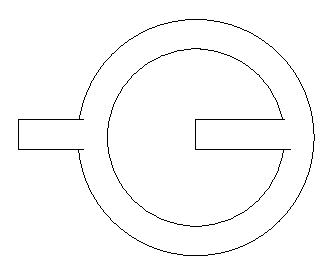
\includegraphics{open-loop.eps}
  \caption{open string$B$N%k!<%W(B}
  \label{open-loop}
 \end{minipage}
 \begin{minipage}[b]{75mm}
  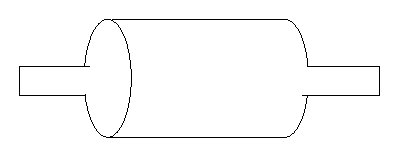
\includegraphics{closed-loop.eps}
  \caption{closed string$B$NEAGE(B}
  \label{closed-loop}
 \end{minipage}
\end{figure}
\ref{perturbation}$B@a$G8+$?$h$&$K!"Hs2D49>l$NM}O@$N7W;;$G$O%@%$%"%0%i%`$r(B
2$B=E@~$K$9$k$H$$$&<jB3$-$r<h$k!#$3$l$O!"(Bopen string$B$H$N%"%J%m%8!<$rM=46$5(B
$B$;$k$b$N$G$"$k!#(B

$B89M}O@$G$N(Bopen string$B$N(B1-loop($B?^(B\ref{open-loop})$B$N%@%$%"%0%i%`$N(BUV$BNN0h$O!"(B
$B%b%8%e%i!<JQ49$K$h$C$F(Bclosed string$B$NEAGE(B($B?^(B\ref{closed-loop})$B$H7k$S$D$$(B
$B$F$$$k$,!"(B$g^{\mu\nu}$$B$r(Bclosed string $B$N%a%H%j%C%/$H$7$F(Bclosed string$B$N(B
$BEAGE$O!"(B
\begin{equation}
 \frac{1}{p_\mu g^{\mu\nu}p_\nu}
\end{equation}
$B$H$$$&FC0[@-$r;}$C$F$$$k!#(B

$BHs2D496u4V$N>e$N>l$r(Bopen string$B$H;W$C$?;~$K!"?^(B\ref{open-loop}$B$N$h$&$J(B
open string$B$N(B1-loop$B$KBP1~$9$k7W;;$OHs2D49(B$\phi^3$$BM}O@$N(B1-loop$B$N(Bnonplanar 
$B$J(B2$BE@4X?t$KBP1~$9$k!#$3$N(Bopen string$B$N(B1-loop$B$KBP1~$9$k(Blosedstring$B$NEAGE(B
$B$NFC0[@-$O(B
\begin{equation}
 \label{nc-field-closed}
 g_{\mu\nu}\sim-(\theta^2)_{\mu\nu}
\end{equation}
$B$H$7$?;~$K!"<0(B(\ref{phi3-eff})$B$NM-8z:nMQ$K$"$kFC0[@-$H0lCW$7$F$$$k!#$3$N(B
$B4X78$O!"8e$K(B\ref{low-energy}$B@a$G5a$a$k(BSeiberg Witten$B6K8B(B(\ref{SW-limit})
$B$G$N(Bopen string$B$N%a%H%j%C%/$H(Bclosed string$B$N%a%H%j%C%/$N4X78<0(B
(\ref{SW-rel})$B$r5a$a$k$,!"$=$3$G(Bopen string$B$N%a%H%j%C%/$r(B$\delta^{ij}$$B$H(B
$B$7$?;~$N(Bclosed string$B$N%a%H%j%C%/$K0lCW$9$k!#(B

%%%%%%%%%%%%%%%%%%%%%%%%%%%%%%%%%%%%%%%%%%%%%%%%%%%%%%%%%%%%%%%%%%%%%%%%
\subsection{Seiberg-Witten $B<LA|(B}
\label{Seiberg-Witten-Map}

$\theta$$B$,0lDj$JHs2D49(B$U(N)$$B%2!<%8M}O@$O<B$O!">l$N:FDj5A$G2D49$J6u4V$N>e(B
$B$N(B$U(N)$$B%2!<%8M}O@$K$J$k$3$H$,CN$i$l$F$$$k(B
\cite{STandNCG}\cite{ComGaugeEquivNCG}$B!#$=$NM}M3$N@bL@$O!"89M}O@$NOHAH$N(B
$BCf$G@bL@$5$l$k$,$3$3$G$O$=$N$h$&$J>l$N:FDj5A$,B8:_$9$k$H$7$F!">l$N:FDj5A(B
$B$r5a$a$F$_$k!#(B

$B$b$7!"Hs2D49%2!<%8M}O@$H2D49%2!<%8M}O@$N4V$K>l$N:FDj5A$G7k$P$l$?4X78$,$"$C(B
$B$?$H$9$l$P!"$=$N>l$N:FDj5A$O0J2<$N$h$&$J?^<0$r2D49$K$7$J$/$F$O$J$i$J$$!#(B
\begin{equation}
 \label{seiberg-witten-diagram}
 \xymatrix{
  \Ah (A)\ar[r]^{\delh_{\lamh}}&\Ah (A+\delta_\lambda A)\\
  A\ar[u]\ar[r]^{\delta_\lambda}&A+\delta_\lambda A\ar[u]}
\end{equation}
$B$?$@$7!"(B$\Ah,\delh,\lamh$$B$O$=$l$>$l!"Hs2D49@-(B$\theh$$B$rF~$l$?Hs2D49%2!<%8(B
$BM}O@$N%2!<%8>l(B,$B%2!<%8JQ49(B,$B%2!<%8JQ49$N%Q%i%a!<%?$G$"$k!#$9$J$o$A!">l$N:F(B
$BDj5A$H%2!<%8JQ49(B($B<0(B(\ref{nc-gauge-transf}))$B$O2D49$G$J$/$F$O$J$i$J$$!#$5(B
$B$i$K$3$N4X78$O0lHL$K0[$J$k(B$\theta$$B$NHs2D49%2!<%8M}O@$,$*8_$$$K>l$N:FDj5A(B
$B$G7k$S$D$$$F$$$k$3$H$r$7$a$7$F$$$k!#$3$N$H$-!"?^<0(B
(\ref{seiberg-witten-diagram})$B$KBP1~$9$k$b$N$r<0$G=q$-8=$o$9$H<!$N$h$&$K(B
$B$J$k!#(B
\begin{equation}
 \Ah(\At)+\delh_\lamh\Ah(\At)=\Ah(\At+\delt_\lamt)
\end{equation}
$BFC$K!"(B
\begin{equation}
  \thet=\theh+\delta\theta \Longrightarrow
   \left\{\begin{array}{l}
    \Ah=\At+\delta\At(\At)+\Ord(\delta\theta^2) \\
    \lamh=\lamt+\delta\lamt(\lamt)+\Ord(\delta\theta^2) \\
   \end{array}\right.
\end{equation}
$B$H$9$k$H>e<0$O!"<!$N$h$&$K$J$k!#(B
\begin{equation}
 \delh_\lamh\delta\At_i-\Dt_i\delta\lamt+i[\delta \Ah_i,]
  =-\1half\delta\theta^{kl}\{\partial_k\At_i,\partial_l\lamt\}
\end{equation}
$B$3$N<0$O(B
\begin{subequations}
 \begin{eqnarray}
  \delta\Ah_i&=&-{1\over 4}\delta\theta^{kl}\{\At_k,\partial_l\At_i+
   \Ft\}+\alpha\delta\theta^{kl}\Dt_i\Ft_{kl}+\beta\delta\theta^{kl}
   \Dt_i[\At_k,\At_l] \\
  \delta\lamt&=&{1\over 4}\delta\theta^{kl}\{\partial_k\lamt,\At_l\}
   +2\beta\delta\theta^{kl}[\partial_k\lamt,\At_l] \\
  \delta\Ft&=&{1\over 4}\delta\theta^{kl}
   \left(2\{\Ft_{ik},\Ft_{jl}\}-\{\At_k,\Dt_l\Ft_{ij}
    +\partial_l\Ft_{ij}\}\right) \nonumber \\
  &&-i\alpha\delta^{kl}[\Ft_{ij},\Ft_{kl}]
   -i\beta\delta\theta^{kl}[\Ft_ij,[\At_k,\At_l]]
 \end{eqnarray}
\end{subequations}
$B$K$h$C$F2r$/$3$H$,$G$-$k!#$3$3$GLLGr$$$N$O!"(B$\alpha,\beta$$B$H$$$&%Q%i%a!<(B
$B%?$NB8:_$G$"$k!#$3$N%Q%i%a!<%?$NB8:_<+BN$O<B$OIT;W5D$G$O$J$$!#2?8N$J$i!"(B
$B$R$H$D$NHyJ,J}Dx<0$r2r$/0Y$K(B3$B$D$N4X?t$r;H$C$F$$$k$+$i$G$"$k!#(B
$\alpha,\beta$$B$KHfNc$9$k9`$O%2!<%8JQ49$N7A$r$7$F$$$k!#$7$?$,$C$F!"$3$N(B
$\alpha,\beta$$B$K$h$kITDj@-$O%2!<%8JQ49$G5[<}$9$k$3$H$,$G$-!"J*M}E*$K$O0U(B
$BL#$N$J$$$b$N$G$"$k!#(B

$B$3$l$GHy>.NL$N(B$\theta$$B$NJQ2=$K$D$$$F$O2r$,5a$^$C$?$,!"$3$N2r$,M-8B$N(B
$\theta$$B$NJQ2=$K$D$$$F$&$^$/Dj5A$G$-$F$$$k$+!"B($A2D@QJ,$G$"$k$+$I$&$+$O(B
$B<+L@$G$O$J$$!#7W;;$r$9$k$H<B$O!"2D@QJ,$G$O$J$$$3$H$,J,$+$k!#$=$N$3$H$r3N(B
$B$+$a$k0Y$K$OFs$D$N(B$\theta$$B$NHy>.JQ2=(B$\delta\theta_1,\delta\theta_2$$B$N8r(B
$B49;R(B$[\delta_1]$$B$,>C$($k$3$H$r8@$o$J$/$F$O$J$i$J$$!#$3$N8r49;R$NI=<0$OHs(B
$B>o$KD9$$$N$G6qBNE*$J7A$O=q$+$J$$$,(B($B6qBNE*$J7A$O(B\cite[$B<0(B
(7)]{ComGaugeEquivNCG}$B$r;2>H!#(B)$B!"BgBN<!$N$h$&$J7A$r$7$F$$$k!#(B
\begin{equation}
 [\delta_1,\delta_2]\At_i=\delta\theta_1\delta\theta_2(\cdots)
  +\Dt_i(\delta\theta_1\delta\theta_2\cdots)
  +\mbox{$\alpha,\beta$$B0MB89`(B}
\end{equation}
$\alpha,\beta$$B0MB89`$O$^$?%2!<%8JQ49$N7A$r$7$F$$$k$N$GJ*M}E*$G$O$J$$$,!"(B
$B$=$l0J30$O%2!<%8JQ49$G>C$($J$$!#$3$l$O(B$\theta$$B$N6u4V$NCf$NJD2sO)$r2s$C$F(B
$BLa$C$F$/$k$H$b$H$N%2!<%850F;$H0[$J$k50F;$K9T$C$F$7$^$&$3$H$r<($7$F$$$k!#(B

 
%\section{$BHs2D49=ENOM}O@(B}
%\label{ncgravity}
%%#! platex master.tex


%%
%% Emergence of NCG in string theory
%%
\chapter{$B89M}O@$K8=$l$kHs2D494v2?3X(B}
\label{emergence}
%#!platex master.tex

$\ref{introduction}$$B>O$N>R2p$G$b=R$Y$?DL$j!"89M}O@$G$OMM!9$JB&LL$KHs2D49(B
$B4v2?E*$J@-<A$,8=$o$l$k!#$7$+$7!"85!989M}O@$O2D49$J;~6u$N>e$GDj5A$5$l$F$*(B
$B$j$=$NHs2D49@-$O1#$5$l$F$$$k!#89M}O@$KHs2D49@-$rF3F~$9$k:G$b4JC1$JJ}K!$O!"(B
$B_{\mu\nu}\not= 0$$B$NGX7J>l$rF~$l$?3+89$NM}O@$r9M$($k$3$H$G$"$k$,!"$3$l(B
$B$O$?$@C1$K<'>l$rF~$l$?Cf$G$NJ*M}$r9M$($k$h$&$J$b$N$G$"$j!"$?$@$N%1!<%9%9(B
$B%?%G%#$G$7$+$J$$2DG=@-$,9b$$(B($BL5O@!"89M}O@$OHs@]F0O@E*$K$O(B$B_{\mu\nu}$$B$,(B
$B$"$k??6u(B($BGX7J>l(B)$B$rA*Br$9$k$H$$$&2DG=@-$b$"$k!#(B)$B!#$7$+$7!"89M}O@$K$h$C$F(B
$BDj5A$5$l$k=ENOM}O@$r(BString Geometry$B$H8F$V$3$H$K$9$l$P!"(BString Geometry$B$O(B
$B??6u(B($BGX7J>l(B)$B$NA*Br$N;EJ}$K0M$i$:$KK\<AE*$KHs2D494v2?$G$"$kK5>Z$,$$$/$D$+(B
$B$"$k!#$3$N>O$G$O$=$N$h$&$J>Z5r$K$J$k$H;W$o$l$k$h$&$J;v<B$r$$$/$D$+Ns5s$9(B
$B$k(B(\ref{uncertainty}$B@a(B\ten\ref{homologytoktheory}\ten\ref{string-field}
$B@a(B$\cdots$)$B!#(B

$B$^$?!"0U?^E*$K??6u$rA*$s$@7k2L$H$7$FF@$i$l$k89M}O@$NJ*M}$K$bLLGr$$E@$,$$$/(B
$B$D$+$"$k$N$G!"$=$l$b>R2p$9$k!#(B(\ref{soliton}$B@a(B\ten\ref{low-energy}$B@a(B)$B!#(B

\section{Space-Time Uncertainty}
 \label{uncertainty}
 %#!platex master.tex

$B89M}O@$K;~4V$H6u4V$NIT3NDj@-4X78$,$"$k$3$H(B\cite{STandS-TUnCertainty}$B$O!"(B
$B89M}O@$NK\<A$KHs2D494v2?3X$,4X$o$C$F$$$k$3$H$N6/NO$JK5>Z$G$"$k!#B($A!"$3(B
$B$N@a$N<089M}O@$K8=$l$kIT3NDj@-$N<0(B\ref{uncertainty-inequality}$B$O2D49$J;~(B
$B6u$N>e$G$O5/$-F@$J$$$3$H$G$"$k!#89M}O@$NHs2D494v2?3XE*$JB&LL$N:G=i$NNc$H(B
$B$7$F$3$N(BSpace-Time Uncertainty$B$r@bL@$9$k!#(B

\subsection{$BD>46E*$JF3=P(B}
$B89M}O@$K$O;~4V$H6u4V$NIT3NDj@-4X78$,$"$k$3$H$,CN$i$l$F$$$k!#:G=i$K!"$*$*(B
$B$6$C$Q$K$=$l$r@bL@$9$k!#$3$NIT3NDj@-4X78$OD>4QE*$K$O!"NI$/CN$i$l$F$$$k%((B
$B%M%k%.!<$H;~4V$NIT3NDj@-$+$i@bL@$9$k$3$H$,$G$-$k!#(B
\begin{equation}
 \Delta E\Delta T \gtrsim 1
\end{equation}
$B89M}O@$G$O!"9b$$%(%M%k%.!<$r;}$C$?89$O9b$$Ne5/%b!<%I$r89$,;}$D$3$H$G<B8=(B
$B$G$-$k!#9b$$Ne5/%b!<%I$r;}$C$?89$O89$HD>8r$9$kJ}8~$K$h$j9-$/6u4V$K9-$,$C(B
$B$F$$$k!#$f$($KBg;(GD$K8@$C$F!"(B
\begin{equation}
 \label{uncertainty-inequality}
 \Delta X\Delta T \gtrsim \ls^2
\end{equation}
$B$H$$$&$3$H$,8@$($k!#$3$l$,;~4V$H6u4V$NIT3NDj@-4X78$G$"$k!#Cm0U$9$Y$-$O!"(B
$B$3$N4X78$O!"NL;RO@$NIT3NDj@-4X78$r89M}O@$N8@MU$r;H$C$F2r<a$7D>$7$?$b$N$G(B
$B$"$k$H$$$&$3$H$G$"$k!#(B

$B9b$$Ne5/%b!<%I$,6u4VJ}8~$K$h$j9-$/9-$,$C$F$$$k$3$H$r$b$&>/$7@:L)$K8+$F$_(B
$B$k!#:#!"KX$I(B$SL(2,\Cplx)$$B??6u$K$"$k$h$&$J89(B1$B$NC<(B($\sigma=0$)$B$K1?F0NL(B$p$
$B$r;}$C$?89(B2$B$,$/$C$D$/2aDx$r9M$($k!#89(B1$B$KA^F~$5$l$k1i;;;R$O!"(B$\exp(ip_\mu
X^\mu(0,\tau))$$B$N7A$r$7$F$$$k!#$h$C$F!"(BX$B$N%b!<%IE83+(B
\begin{equation}
 X^\mu=x^\mu-i{2\ls^2p^\mu\over 2}+i\left({\ap\over2}\right)^{1\over 2}
  \sum_n\left({\alpha^\mu_n\over n z^n}\right)
\end{equation}
$B$r9M$($k$H!"$3$N89(B2$B$,$/$C$D$/$3$H$K$h$C$F89(B1$B$N>uBV$O!"(B
\begin{equation}
 \ket{\Psi}\equiv \E^{\sum_np\alpha_{-n}\ls\diagup n}\ket{0}
\end{equation}
$B$X$HJQ2=$9$k!#$f$($K89(B2$B$,$/$C$D$/$3$H$K$h$C$F!"89(B1$B$N6u4VJ}8~$N3H$,$j$O0J(B
$B2<$N$h$&$K$J$k!#(B
\begin{eqnarray}
 \label{DeltaX}
 \Delta X &\sim& \sqrt{\int d\sigma \bra{\Psi}X(\sigma)^2\ket{\Sigma}}
  \nonumber \\
 &\sim& \sqrt{\int d\sigma \bra{0}\sum_n(p^2\ls^2{1\over n})^2
  \E^{p^2\ls^2\over 2n}\ket{0}} \nonumber \\
 &\sim& \sqrt{p^2\ls^4\sum_n({1\over n^2})} \nonumber \\
 &\sim& E\ls^2
\end{eqnarray}
$B5$$rIU$1$M$P$J$i$L$N$O!"$3$N<0$O6u4VJ}8~$N$_$J$i$:;~4VJ}8~$K$b3H$,$j$,$"(B
$B$k$3$H$r<($7$F$$$k$h$&$K8+$($k$3$H$G$"$k!#$3$l$O!"KAF,$K=P$FMh$?(B$\Delta
T$$B$H$N:.F1$r0z$-5/$3$7$+$M$J$$!#$7$+$7!"@h$K=R$Y$?(B$\Delta T$$B$O!"Aj8_:nMQ(B
$B$,5/$-$k;~4V$G$"$j!"89$N=E?4$N;~4V$GDj5A$5$l$F$$$k$3$H$KCm0U$9$l$P!"<0(B
(\ref{DeltaX})$B$G$N;~4VJ}8~$N3H$,$j$H!"(B$\Delta T$$B$OF1$8$b$N$G$O$J$$$3$H$,(B
$BJ,$+$k!#(B

\subsection{$B6&7ABP>N@-$H(BSpace-Time Uncertainty}

$B<B$O!"(BSpace-Time Uncertainty$B$N5/8;$O(Bworld sheet$B$N6&7AITJQ@-$K$"$k!#(B
\cite{InterpretMinLenST}$B$=$N$3$H$r8+$k0Y$K$O$^$:!"6&7AITJQ$J5wN%$NB,$jJ}(B
$B$rDj5A$7$J$/$F$O$J$i$J$$!#(B$ds=\rho(z,\zb)$$B$H$7$F$"$kM-8B$JNN0h(B$\Omega$$B$H(B
$B$=$NNN0h$NCf$N;OE@$H=*E@$rF1$8$/$9$k$h$&$J7PO)$N=89g(B$\Gamma$$B$K$D$$$F6&7A(B
$BITJQ$J5wN%(B(extremal length)$B$O0J2<$N$h$&$KDj5A$5$l$k!#(B
\begin{equation}
 \label{extremal-length}
 \lambda_\Omega(\Gamma)=\sup_\rho
  \frac{\left(\inf_{\gamma\in\Gamma}\int_\gamma\,\rho|dz|\right)}{
  \int_\Omega\, \rho^2|dz|^2}
\end{equation}

\begin{figure}[ht]
 \begin{center}
  \input{conformal-region.pstex_t}
  \caption{$B6&7AITJQ$J5wN%(B}
  \label{region}
 \end{center}
\end{figure}
$B$$$^!"(Bworld sheet$B>e$NNN0h(B$\Omega$$B$H$7$F(B$\alpha,\alpha',\beta,\beta'$$B$G0O(B
$B$^$l$kD9J}7A$NNN0h$r9M$($k!#$9$k$H!"(B$\alpha$$B$H(B$\alpha'$$B$N4V$N7PO)$N=89g(B
$\Gamma$$B$H(B$\beta$$B$H(B$\beta'$$B$N4V$N7PO)$N=89g(B$\Gamma^*$$B$,B8:_$7$F!"99$K!"(B
$\alpha,\alpha'$$B$N4V$N(BEuclid$B5wN%$r(B$a$$B!"(B$\beta,\beta'$$B$N4V$N(BEuclid $B5wN%$r(B
$b$$B$H$9$l$P!"(B
\begin{equation}
 \lambda_\Omega(\Gamma)=\frac{b}{a},\quad
  \lambda_\Omega(\Gamma^*)=\frac{a}{b}
\end{equation}
$B$G$H$J$k!#99$K!"(B
\begin{equation}
 \label{gen-uncertainty}
 \lambda_\Omega(\Gamma) \lambda_\Omega(\Gamma^*)=1
\end{equation}
$B$,8@$($k!#$3$l$O!"(B
\begin{equation}
 \lambda_\Omega(\Gamma) \leq 1\quad\mbox{or}
  \quad\lambda_\Omega(\Gamma^*)\leq 1
\end{equation}
$B$G$"$k$3$H$r<($7$F$$$F!"$3$l$,(BSpace-Time uncertainty$B$N5/8;$K$J$C$F$$$k!#(B
$B$=$N$3$H$r8+$k$K$O!"NN0h(B$\Omega$$B$K(BDirichlet$B6-3&>r7o!"(B
\begin{eqnarray}
 X^\mu(0,\tau)&=X^\mu(a,\tau)&=\delta^{\mu 2}\frac{B\tau}{2} \\
 X^\mu(\sigma,0)&=X^\mu(\sigma,b)&=\delta^{\mu 1}\frac{A\sigma}{2}
\end{eqnarray}
$B$r2]$9$H!"89M}O@$N7PO)@QJ,(B
\begin{equation}
 \int [dx^\mu] \exp\left(-\frac{1}{4\pi\ls^2}\int d\sigma d\tau
	(-\gamma)^{1\diagup 2}\gamma^{ab}
	\partial_a X^\mu \partial_b X_\mu \right)
\end{equation}
$B$+$i!"(B$A,B$$B0MB8@-$H$7$F!"<!$N$h$&$J9`$,=P$FMh$k!#(B
\begin{equation}
 \E^{-\frac{1}{4\pi\ls^2}(A^2\lambda_\Omega(\Gamma)
  +B^2\lambda_\Omega(\Gamma^*))}
\end{equation}
$B:#!"(B$A$$B$H(B$B$$B$rJQ2=$5$;$k$3$H$r9M$($k!#(B$\Delta A,\Delta B$$B$r7PO)@QJ,$K1F(B
$B6A$rM?$($F$7$^$o$J$$$h$&$J(B$A,B$$B$NJQ2=$NI}$HDj5A$9$k$H!"<0(B
(\ref{gen-uncertainty})$B$h$j!"(B
\begin{equation}
 \label{a-b-uncertainty}
 \Delta A \Delta B \sim \ls^2
\end{equation}
$B$,F3$+$l$k!#$9$J$o$A!"$"$k(B2$B<!85E*$J;~6u>e$N9-$,$j$K89$r8GDj$9$k$3$H$r9M(B
$B$($?;~$K!"$=$N8GDj$9$kNN0h$NI}$,<0(B(\ref{a-b-uncertainty})$B$rK~$?$9;~$K=i(B
$B$a$FJ*M}$K1F6A$r5Z$\$9$H$$$&$3$H$,J,$+$k!#(B


%\section{Matrix Theory$B$NHs2D494v2?3XE*B&LL(B}
% \label{matrix}
% %#!platex master.tex

$B9TNsLO7?(B\cite{IKKTMatrix}\cite{BFSSMatrix}$B$O89M}O@$N9=@.O@E*$JDj<02=$H$7(B
$B$FDs>'$5$l$F$$$k$b$N$G$"$k!#9TNsLO7?$H89M}O@5Z$S$=$NHs@]F0O@E*Dj<02=$H$N(B
$B4V$N4X78$OI,$:$7$bL@$i$+$G$O$J$$$,!"9TNsLO7?$,Hs@]F0O@E*$JDj<02=$K$J$C$F(B
$B$$$k$H$$$&>Z5r$O$$$/$D$+$"$k!#%H!<%i%9%3%s%Q%/%H2=$5$l$?9TNsLO7?$+$i$OHs(B
$B2D494v2?3X$,<+A3$K8=$o$l$k$3$H$,CN$i$l$F$$$k!#$3$l$O!"Hs2D494v2?3X$,89M}(B
$BO@$NHs@]F0O@E*Dj<02=$K?<$/4X$o$C$F$$$k$3$H$N$R$H$D$N>Z5r$G$"$k!#(B


\subsection{IKKT$B9TNsLO7?(B}
$B9TNsLO7?$K$O(BIIA$B9TNsLO7?$H(BIIB$B9TNsLO7?$N(B2$B$D$NN.57$,$"$k$,!"$^$:$O(BIIA$B9TNsLO(B
$B7?$+$i@bL@$9$k!#(BIIA$B9TNsLO7?$N:nMQ$O!"<!$GM?$($i$l$k!#(B

\section{String Field Theory$B$NHs2D494v2?3XE*B&LL(B}
 \label{string-field}
 %#!platex master.tex

String Field Theory$B$HHs2D494v2?3X$H$N4X78$OAa$/$+$i;XE&$5$l$F$-$?(B
\cite{NCGandSFT}$B!#$3$N@a$G$O(BString Field Theory$B$N7W;;J}K!$N>\:Y$K$O?($l(B
$B$:$K$=$NHs2D494v2?3XE*$JB&LL$@$1$K9J$C$F@bL@$9$k!#(BString Field Theory$B$N(B
$B7W;;J}K!$N>\:Y$K$D$$$F$O!"Bg?9$N=$;NO@J8(B\cite{OhmoriMthesis}$B$r;2>H!#(B

\subsection{Open String Field Theory$B$N%i%0%i%s%8%"%s(B}

String Field Theory$B$r9M$($k$KEv$C$F!"I,MW$J$b$N$r9M$($k$H(BString Field$B$N(B
$B@.$9Be?t!"89F1;N$NAj8_:nMQ!"(BBRST$BJQ49(B(BRST$B7A<0$G9M$($J$1$l$P$J$i$J$$M}M3(B
$B$O8e$K@bL@$9$k!#(B)$B!"6u4V>e$N@QJ,$J$I$,9M$(IU$/!#$=$3$G!"$^$:Cj>]E*$K(B
$\Intg_2$graded$B$G0lHL$K$OHs2D49$JBe?t(B$\AlgB$$B$H$=$N>e$N@Q(B$*$ $B$=$7$F!"$=$N(B
$B>e$N(Bodd$B$JHyJ,(B$Q$$B$H@QJ,(B$\int$$B$r9M$($k!#(B$A,B\in\AlgB$$B$H$7$F$=$l$i$N(Bgrade$B$r(B
$a,b\in \{0,1\}$$B$H=q$/$3$H$K$9$k!#$3$N;~!"$3$NBe?t$O!"0J2<$N$h$&$J4X78<0(B
$B$rK~$?$7$F$$$k$H2>Dj$9$k!#(B
\begin{align}
 \mathrm{grade}(A*B)&\equiv a+b\quad(\mathrm{mod}2) \\
 \mathrm{grade}(Q(A))&\equiv a+1\quad(\mathrm{mod}2) \\
 Q(Q(A))&=0 \\
 Q(A*B)&=Q(A)*B+(-1)^aQ(B) \\
 \int A*B&=(-1)^{ab} \int B*A \\
 \int Q(A)&=0
\end{align}
$BNc$($P(B$\AlgB$$B$rHyJ,7A<0(B$Q,*,\int$$B$r$=$l$>$l30HyJ,(B\ten wedge$B@Q(B\ten $B@QJ,$H(B
$B$9$l$P>e$N@-<A$rK~$?$9!#$3$3$G!"@Q(B$*$$B$O(Bwedge$B@Q(B$\wedge$$B$N0lHL2=$G(Bwedge$B@Q(B
$B$H9TNs$N@Q$NAH$_9g$;$K$J$C$F$$$k$+$b$7$l$J$$$H$$$&$3$H$K8@5Z$7$F$*$/!#(B

$B99$K!"(B$\AlgB_0\subset\AlgB$$B$H$$$&(B$*$$B@Q$K$h$C$FJD$8$?ItJ,Be?t$,$"$k$H$9$k!#(B
$B$3$l$O!"(B0-$B7A<0$N0lHL2=$G$"$k!#(B$A_i,B_j,C_k\in\AlgB_0$$B$K$D$$$F(B$n$-$B7A<0$r(B
\begin{equation}
 \sum_{i,j,k} A_i*Q(B_j)*\cdots*Q(C_j)
\end{equation}
$B$K$h$C$FDj5A$9$k!#(B

$B$3$l$i$NDj5A$K$h$C$F%2!<%8M}O@$N0lHL2=$rDj5A$9$k$3$H$,$G$-$k!#$9$J$o$A!"(B
1-$B7A<0(B$A$$B$N(B$\epsilon\in\AlgB_0$$B$r%Q%i%a!<%?$H$7$F%2!<%8JQ49$r(B
\begin{equation}
 \delta_\epsilon A\equiv Q(\epsilon)+A*\epsilon-\epsilon *A
\end{equation}
$B$HDj5A$7!"(Bfield strength$B$r(B
\begin{equation}
 F\equiv Q(A)+A*A
\end{equation}
\begin{equation}
 \delta_\epsilon F=F*\epsilon -\epsilon *F
\end{equation}
$B$HDj5A$9$k!#$3$3$G!"(Bfield strength$F$$B$O(BBianchi$BEy<0(B
\begin{equation}
 Q(F)+A*F-F*A=0
\end{equation}
$B$rK~$?$9!#$3$N%2!<%8M}O@$N%i%0%i%s%8%"%s$H$7$FE,Ev$J%i%0%i%s%8%"%s$O!"8=(B
$B:_<j85$K$"$k@Q$,(Bwedge$B@Q$KBP1~$9$k$b$N$7$+$J$$$N$G!"(BChern-Simons$B7?$,E,Ev(B
$B$G$"$k!#B($A!"(B
\begin{equation}
 \label{chern-simons-action}
 I=\int(A*Q(A)+\frac{2}{3}A*A*A)
\end{equation}
$B$3$N%i%0%i%s%8%"%s$+$i5a$^$k1?F0J}Dx<0$O!"(B
\begin{equation}
 \label{chern-simons-eom}
 F=0
\end{equation}
$B$H$J$k!#$b$7!"(B$A$$B$r$?$@$N%2!<%8>l$H$7$F8+$?>l9g$3$N<0$OHs>o$K<+L@$9$.$F(B
$BM}O@$H$7$F$NLLGr$_$N7g$1$k$b$N$H$J$k!#$7$+$7!"(B$A$$B$r(B$a\xrightarrow{A}A*a$ 
$B$J$k1i;;;R$@$H;W$&$3$H$K$9$l$P!"(B(\ref{chern-simons-eom})$B$O(B$a$$B$X$N:nMQ$r(B
$B9M$($l$P!"(B
\begin{align}
 (Q(A)+A*A)a&=Q(Q(a))+Q(A*a)+A*Q(a)+A*A*a \nonumber \\
 &=(Q+A)^2a=0
\end{align}
$B$H$J$k!#(B

$BCj>]E*$JBe?t$NDj5A$r$9$kA0$K=R$Y$?$h$&$K!"89M}O@$NJ8L.$G$O(B$Q$$B$O(BBRST$BJQ49(B
$B$H$7$F2r<a$5$l!"$^$?Dj5A$N$h$&$J@-<A$rK~$?$9(B$Q$$B$N8uJd$O(BBRST$BJQ49$7$+$J$$(B
$B$N$G!"(B$(Q+A)$$B$O?7$?$J(B(1+1)$B<!85$NM}O@$Nf2Nm$J(BBRST$B1i;;;R$H2r<a$5$l$k!#(B

\subsection{String field$B$N(Bassociativity}

String Field Theory$B$r9=@.$9$k:]$K(BString Field $B$NBe?t$,7k9gN'$rK~$?$9$+$I(B
$B$&$+!"B($A(B
\begin{equation}
 U*(V*W)=(U*V)*W
\end{equation}
$B$,@.N)$9$k$+$I$&$+$O!"HyL/$JLdBj$G$"$k!#<B:]!"(Bopen string$B$N@.$9Be?t$O7k(B
$B9gN'$rK~$?$9$,!"(Bclosed string$B$N@.$9Be?t$,7k9gN'$rK~$?$5$J$$!#$^$:$O$=$N(B
$B$3$H$r@bL@$7$F$$$/!#(B

\begin{figure}[ht]
 \begin{minipage}[b]{75mm}
  \begin{center}
   \input{open-interaction-1.pstex_t}
   \caption{$BC1=c$J(Bopen string$B$NAj8_:nMQ(B}
   \label{open-interaction-1}
  \end{center} 
 \end{minipage}
 \begin{minipage}[b]{75mm}
  \begin{center}
   \input{open-associativity.pstex_t}
   \caption{$BC1=c$J(Bopen string$B$NAj8_:nMQ$N7k9g@-(B}
   \label{open-interaction-associativity}
  \end{center} 
 \end{minipage}
\end{figure}
open string$B$N>l$NAj8_:nMQ$H$7$F$b$C$H$bC1=c$J$N$O!"0lJ}$N89$N:8C<$H$b$&(B
$B0lJ}$N89$N1&C<$r$/$C$D$1$k!"?^(B\ref{open-interaction-1}$B$N$h$&$JAj8_:nMQ$r(B
$B9M$($k$3$H$G$"$k!#$3$NAj8_:nMQ$GDj5A$5$l$k@Q$OL@$i$+$KHs2D49$G$"$k$,!"7k(B
$B9gN'$OK~$?$7$F$$$k!#(B

\begin{figure}[ht]
 \begin{minipage}[b]{75mm}
  \begin{center}
   \input{closed-interaction.pstex_t}
   \caption{closed string$B$NAj8_:nMQ(B}
   \label{closed-interaction}
  \end{center} 
 \end{minipage}
 \begin{minipage}[b]{75mm}
  \begin{center}
   \input{closed-associativity.pstex_t}
   \caption{closed string$B$NAj8_:nMQ$N7k9g@-(B}
   \label{closed-interaction-associativity}
  \end{center} 
 \end{minipage}
\end{figure}
$B0lJ}!"(Bclosed string$B$N>l9g$O!"Aj8_:nMQ$H$7$F$O!"89$N(B1$BE@$r$/$C$D$1$k$h$&$J(B
$B?^(B\ref{closed-interaction}$B$N$h$&$JAj8_:nMQ$r9M$($k$N$,<+A3$G$"$k!#$3$NAj(B
$B8_:nMQ$K$h$k@Q$O(Bopen string$B$N;~$N$h$&$K:81&$N6hJL$,L5$$$N$G2D49$J@Q$K$J$C(B
$B$F$$$k!#$7$+$7!"?^(B\ref{closed-interaction-associativity}$B$N$h$&$J(B3$B$D$N(Bopen
string$B$NAj8_:nMQ$r9M$($k$H!"(B$U*V$$B$O$*8_$$$K8r$o$C$F$$$J$$$N$G(B$0$$B$K$J$k$+(B
$B$i!"(B$0=(U*V)*W\neq U*(V*W)$$B$G$"$j!"@Q$N7k9gN'$,2u$l$F$7$^$C$F$$$k!#(B

\subsection{open string$B$NAj8_:nMQ$N=$@5(B}

\begin{figure}[ht]
 \begin{minipage}[b]{75mm}
  \begin{center}
   \input{open-reparametrization-1.pstex_t}
   \caption{(U*V)$B$r@h$K$d$C$?>l9g(B}
   \label{open-repara-1}
  \end{center} 
 \end{minipage}
 \begin{minipage}[b]{75mm}
  \begin{center}
   \input{open-reparametrization-2.pstex_t}
   \caption{(V*W)$B$r@h$K$d$C$?>l9g(B}
   \label{open-repara-2}
  \end{center} 
 \end{minipage}
\end{figure}
$BA0$N>.@a$G!"(Bclosed string$B$N?^(B\ref{open-interaction-1}$B$N$h$&$JAj8_:nMQ$O(B
$B7k9gN'$rK~$?$9$H$$$C$?$,!"<B$OHyL/$JE@$,$"$k!#$=$l$O!"$3$N7k9g@-$,(Bworld
sheet$B$N:BI8$N:FDj5A$K0M$C$F$$$k$H$$$&E@$G$"$k!#$D$^$j!"?^(B
\ref{open-repara-1}$B$H?^(B\ref{open-repara-2}$B$G<($5$l$F$$$k$h$&$K!"@Q$r9T$J(B
$B$&=g=x$K0M$C$F!"89$NCf$N:BI8$,0[$J$C$F$$$k$H$$$&E@$G$"$k!#(B

$B$7$+$7!"89$N:BI8$N:FDj5A$N<+M3EY$r;D$7$?$^$^(Bstring field theory$B$r9=@.$9(B
$B$k$3$H$OHs>o$KFq$7$$$3$H$,CN$i$l$F$$$k!#:BI8$N:FDj5A$N<+M3EY$r;D$9Be$o$j(B
$B$K(BBRST$B7A<0$K$N$C$H$C$F(BBRST$B%A%c!<%8$NJ]B8$r2]$7$?$[$&$,3Z$G$"$k!#$5$i$K!"(B
$BJL$NLdBj$H$7$F!"?^(B\ref{open-interaction-1}$B$N$h$&$JAj8_:nMQ$r9M$($?;~$K$&(B
$B$^$/@QJ,$rDj5A$G$-$J$$(B($BL5M}LpM}:8C<$H1&C<$r$/$C$D$1$F@QJ,$9$k$H$=$l$O(B
closed string$B$KCM$r<h$C$F$7$^$&!#(B)$B$H$$$&LdBj$,$"$k!#(B

\begin{figure}[ht]
 \begin{center}
  \input{open-interaction-2.pstex_t}
  \caption{$B=$@5$7$?(Bopen string$B$NAj8_:nMQ(B}
  \label{open-interaction-2}
 \end{center}
\end{figure}
$B$3$NFs$D$NLdBj$r2r7h$9$k$?$a$K(Bopen string$B$NAj8_:nMQ$N;EJ}$KJQ99$r2C$($k!#(B
$B$=$N0Y$K!"$^$:!"(Bopen string $S$$B$rH>J,(B($\sigma=\frac{\pi}{2}$)$B$+$i:8$H1&(B
$(U_L,V_R)$$B$KJ,$1$k!#=$@5$5$l$?(Bopen string$B$NAj8_:nMQ$O(B
\begin{equation}
 \label{witten-star}
 (U_L,U_R)*(V_L,V_R)\equiv (U_L,V_R)\delta(U_R-V_L)
\end{equation}
$B$H$$$&7A(B($B?^(B\ref{open-interaction-2})$B$r$7$F$$$k!#$3$l$O!"89$N:BI8$N:FDj5A(B
$B$rI,MW$H$7$J$$0Y$K(BBRST$B7A<0$G%2!<%88GDj$r$7$?$^$^Aj8_:nMQ$r7W;;$G$-$k$N$G(B
$BHs>o$K9%ET9g$G$"$k!#$^$?!"@QJ,$O(B
\begin{equation}
 \int U*V=\delta(U_R-V_L)\delta(U_L-V_R)
\end{equation}
$B$HDj5A$9$k$3$H$,$G$-$k!#$3$N$h$&$J!"(Bopen string$B$NAj8_:nMQ$GDj5A$5$l$?@Q(B
$B$r$3$N@a$N=i$a$KCj>]E*$KDj5A$7$?(B$*$$B$H?7$?$KDj5A$7$F!"(B
(\ref{chern-simons-action})$B$N:nMQ$N2<$K9=@.$5$l$?M}O@$,(BWitten$B7?$N(BOpen
String Field Theory$B$G$"$k!#(B

\subsection{Witten$B$N(BOpen String Field Theory$B$NHs2D49@-(B}

\begin{figure}[ht]
 \begin{center}
  \input{SFT-NC.pstex_t}
  \caption{Witten$B$N(BOpen String Field Theory$B$NHs2D49@-(B}
  \label{SFT-NC}
 \end{center}
\end{figure}
$B:G8e$K!"(BWitten$B$N(BOpen String Field Theory$B$,;}$DHs2D49@-$K$D$$$F@bL@$9$k!#(B
$B$3$N@a$N:G=i$NCj>]E*$J9=@.$+$i!"(Bstring field$B$N@.$9Be?t$O0lHL$KHs2D49$J$b(B
$B$N$G$"$C$?$,!"<B:]?^(B\ref{SFT-NC}$B$+$iD>46E*$KJ,$+$k$h$&$K(BWitten$B$N(BOpen
String Field Theory$B$G(Bstring field$B$N@.$9Be?t$OHs2D49$K$J$C$F$$$k!#B($A!"(B
\begin{equation}
 (U_L,V_R)\delta(U_R-V_L)\neq(V_L,U_R)\delta(V_R-U_L)
\end{equation}
$B$H$J$C$F$$$k!#(B

\section{$B89M}O@$NDc%(%M%k%.!<M-8zM}O@$H(BSeiberg-Witten$B<LA|(B}
 \label{low-energy}
 %#! platex master.tex

D-brane$B$NDc%(%M%k%.!<M-8zM}O@$O(BDirac-Born-Infeld$B:nMQ$G$"$k$3$H$,$[$\3N<B(B
$B;k$5$l$F$$$k!#$3$N@a$G$O!"@h$K=R$Y$?(BSeiberg-Witten$B<LA|$,89M}O@$NDc%(%M%k(B
$B%.!<M-8zM}O@$H$7$F!"3+89$NM}O@$N(Bregularization$B$N0c$$$H$7$F@bL@$G$-$k$3$H(B
$B$r=R$Y$k!#(B

\subsection{$B$$B>l$NB8:_2<$G$N(Bopen-string$B$NM}O@(B}
$B:#(B$B$$B>l$,(B$i=1,\ldots,r$$BJ}8~$K$N$_B8:_$9$k>u67$r9M$($k!#B8:_$9$k;~$N(B
Euclid$B2=$7$?(Bworld sheet$\Sigma$$B>e$N:nMQ$O!"(B
\begin{eqnarray}
 S&=\frac{1}{4\pi\ap}\int_\Sigma(g_{ij})\partial_aX^i\partial^aX^j
  -2\pi i\ap B_{\mu\nu}\epsilon^{ab}\partial_aX^i\partial_aX^j\nonumber\\
  &=\frac{1}{4\pi\ap}\int_\sigma(g_{ij})\partial_aX^i\partial^aX^j
  -\frac{i}{2}\int_{\partial\Sigma}B_{ij}X^i\partial_tX^j
\end{eqnarray}
$B$G$"$k!#:#(Bworld sheet$B$,>eH>J?LL$K$"$k$H$7$F!"(BD-brane$B$K1h$C$?J}8~$N(B
$X^\mu$$B$,K~$?$96-3&>r7o$O1?F0J}Dx<0$h$j!"(B
\begin{equation}
 \label{Dbr-bdry-cond}
 g_{ij}(\partial-\bar{\partial}+2\pi\ap B_{ij}
  (\partial+\bar{\partial})X^j)\Big|_{z=\zb}=0
\end{equation}
$B$G$"$k!#$3$N6-3&>r7o$O!"(B$B=0$$B$N;~$K(BNeumann$B6-3&>r7o$H$J$j!"(B$B=\infty$$B$N;~(B
$B$K(BDirichlet$B6-3&>r7o$H$J$k!#$3$N6-3&>r7o$N2<$G$N(Bpropagator$B$r7W;;$9$k!#:#!"(B
propagator$B$r5a$a$k$KEv$j!"6@A|K!$r;H$&$3$H$r9M$($k$H!"6-3&>r7o$,(B
Dirichret$B6-3&>r7o$H(BNeumann$B6-3&>r7o$N:.9g$K$J$C$F$$$k$3$H$+$i!"(Bpropagator
$B$O!"(B
\begin{equation}
 \langle X^i(z)X^j(z')\rangle=-\ap(g^{ij}\ln|z-z'|
  +C^{ij}\ln(z-\zb')+D^{ij}\ln(\zb-z')+\mathrm{const})
\end{equation}
$B$N7A$K$J$C$F$$$k$O$:$G$"$k!#$3$3$G!"(B$\langle X^i(z)X^j(z')\rangle$$B$N(B
$X^i(z) $$B$K$D$$$F!"<0(B(\ref{Dbr-bdry-cond})$B$rE,MQ$9$k$H!"(B
\begin{multline}
 -(g_{ij}+2\pi\ap B_{ij})g^{jk}\frac{1}{z-z'}
 -(g_{ij}+2\pi\ap B_{ij})C^{jk}\frac{1}{z-\zb'} \\
 +(g_{ij}-2\pi\ap B_{ij})g^{jk}\frac{1}{\zb-\zb'}
  -(g_{ij}-2\pi\ap B_{ij})D^{jk}\frac{1}{z-z'}  =0
\end{multline}
$B$H$J$j!"$3$l$,A4$F$N(B$z'$$B$K$D$$$F@.N)$9$k$3$H$rMxMQ$9$k$H!"(B$C^{ij},
D^{ij}$$B$r5a$a$k$3$H$,$G$-$k!#(B
\begin{align}
 C^{ij}&=\left(\frac{1}{g+2\pi\ap B}\right)^{ij}-\1halfg^{ij} \\
 D^{ij}&=\left(\frac{1}{g-2\pi\ap B}\right)^{ij}-\1halfg^{ij}
\end{align}
$B$3$l$r$^$H$a$k$H!"(Bpropagator$B$N:G=*E*$J7A$O0J2<$N$h$&$K$J$k!#(B
\begin{align}
 \label{open-propag}
 \langle X^i(z)X^j(z')\rangle
  =&-\ap\Big(g^{ij}\log|z-z'|-g^{ij}log|z-\zb'\nonumber\\
 &+G^{ij}\log|z-\zb'|^2+\frac{1}{2\pi\ap}\theta^{ij}log\frac{z-\zb'}{\zb-z'}
  +\mathrm{const}\Big)
\end{align}
$B$3$3$G!"(B$G^{ij},\theta^{ij}$$B$O0J2<$N$h$&$KDj5A$5$l$F$$$k!#JXMx$N0Y$K(Bopen
string$B$N%+%C%W%j%s%0$H(Bclosed string$B$N%+%C%W%j%s%0$N4X78$rIU$12C$($F$*$$$?!#(B
\begin{equation}
 \label{openstring-parameters}
 \left\{
  \begin{array}{l}
   G^{ij}=\left({1\over g+2\pi\ap B}\right)^{ij}_{\hbox{$BBP>N(B}}
    =\left({1\over g+2\pi\ap B}g{1\over g-2\pi\ap B}\right)^{ij} \\
   G_{ij}=g_{ij}-(2\pi\ap)^2(Bg^{-1}B)_{ij} \\
   \theta^{ij}=2\pi\ap\left({1\over g
			+2\pi\ap B}\right)^{ij}_{\hbox{$BH?BP>N(B}}
    =-(2\pi\ap)^2\left({1\over g+2\pi\ap B}
		  B{1\over g-2\pi\ap B}\right)^{ij}\\
   G_s=g_s\left({\det G\over\det(g+2\pi\ap B)}\right)^{\1half}
      =g_s\left({\det G\over\det g}\right)^{1\over 4}
      =g_s\left({\det(g+2\pi\ap B)\over\det g}\right)^{\1half} \\
  \end{array} 
\right.
\end{equation}
$B:#!"6=L#$r;}$C$F$$$k$N$O(Bopen string$B$NAj8_:nMQ$J$N$G!"(B$X^i(z)$$B$O6-3&$N>e(B
$B$K$$$k$H9M$($k!#$9$k$H!"(B$z=\tau\in\Real$$B$HI=5-$9$k$3$H$,$G$-$k$N$G!"(B
propagator$B$N<0$O(B
\begin{equation}
 \label{bdry-propag}
 \langle^i x^i(\tau)x^j(\tau')\rangle=-\ap G^{ij}\log(\tau-\tau')^2
  +\ihalf\theta^{ij}\epsilon(\tau-\tau')
\end{equation}
$B$H$J$k!#$7$?$,$C$F!"(B$G^{ij}$$B$O(Bopen string$B$,46$8$k%a%H%j%C%/$H$$$&$3$H$K(B
$B$J$k!#0lJ}(B$\theta^{ij}$$B$O1i;;;R(B$X^i$$B$N8r49;R$,(Btime ordering$B$NF~$lBX$($K(B
$B$J$C$F$$$k$3$H$r9M$($k$H!"(B
\begin{equation}
 [X^i,X^j]=T(X^i(\tau)X^j(\tau^-)-X^i(\tau)X^j(\tau^+))=i\theta^{ij}
\end{equation}
$B$G$"$k$+$i!"(B$\theta^{ij}$$B$O:BI8$NHs2D49@-$H8+$k$3$H$,$G$-$k!#(B

\subsection{$BDc%(%M%k%.!<M-8zM}O@$X$N(B$B$$B>l$N1F6A(B}

$B89M}O@$N?6I}$N7W;;$r$9$k0Y$K$O!"$"$k1?F0NL$r;}$C$?(Bworld sheet$B>e$N1i;;;R(B
$V(X)\E^{ip \cdot X}$$B$rA^F~$7$?!"?6I}$r7W;;$7$J$/$F$O$J$i$J$$!#$3$3$G(B
$V(X)$$B$O(B$\partial X^i,\der^2X^i,\ldots$$B$+$i$J$kB?9`<0$G$"$k!#(B
\begin{equation}
 \left\langle\prod^n_{i=1}V_i(X(\tau_i))\E^{ip_i\cdot X(\tau_i)}
		       \right\rangle_{G,\theta}
\end{equation}
$B$7$+$7!"$3$N?6I}$O(B$G$$B$rJQ2=$5$;$:$K!"(B$\theta$$B$@$1$r<j$G(B$0$$B$K$7$??6I}$H0J(B
$B2<$N$h$&$J4X78$r$b$C$F$$$k!#(B
\begin{equation}
 \left\langle\prod^n_{i=1}V_i(X(\tau_i))\E^{ip_i\cdot X(\tau_i)}
 \right\rangle_{G,\theta}
 =\E^{-\ihalf\sum_{n>m}p_i\theta^{ij}p_j\epsilon(\tau_n-\tau_m)}
 \left\langle\prod^n_{i=1}V_i(X(\tau_i))\E^{ip_i\cdot X(\tau_i)}
 \right\rangle_{G,\theta=0}
\end{equation}
$B$3$l$O!"1i;;;R$r(B$\tau_n$$B$NBg>.$N=g$KJB$Y$?;~$K(B$\theta=0$$B$NM}O@$H(B$\theta$ 
$B$,M-8B$NM}O@$,!"1?F0NL0MB8ItJ,(B($\E^{ip\cdot X}$)$B$@$1$O!"@Q$rIaDL$N@Q$+$i(B
Moyal$B@Q$KD>$9$3$H$K$h$C$FF@$k$3$H$,$G$-$k$H$$$&$3$H$r<($7$F$$$k!#(B$\E^{i
p\cdot X}$$B$NItJ,$K8BDj$9$l$P!"$^$5$K(B$\theta$$B0lDj$N>l9g$NJQ7ANL;R2=$K$h$k(B
$BHs2D49>l$NM}O@$N9=@.K!$HF1$8$b$N$G$"$k!#(B

\subsection{Seiberg-Witten$B6K8B(B}

$\ap\rightarrow 0$$B$G$NDc%(%M%k%.!<M-8zM}O@$r9M$($?$$$N$@$,!"(Bopen string 
$B$,46$8$k%a%H%j%C%/$dHs2D49@-$OM-8B$KJ]$A$?$$!#$=$3$G!"(Bopen string$B$N%Q%i(B
$B%a!<%?(B(\ref{openstring-parameters})$B$rM-8B$KJ]$D0J2<$N$h$J$&6K8B$r9M$($k!#(B
\begin{equation}
 \label{SW-limit}
 \begin{split}
  \ap\sim\epsilon^{\1half}&\rightarrow 0 \\
  g_{ij}\sim\epsilon&\rightarrow 0\quad\mbox{for}i,j=1,\ldots,r
 \end{split}
\end{equation}
$B$3$N6K8B$r(BSeiberg-Witten limit$B$H$$$&!#$9$k$H!"(Bopen string$B$N%Q%i%a!<%?(B
(\ref{openstring-parameters})$B$O<!$N$h$&$K$J$k!#(B
\begin{equation}
 \label{SW-rel}
 \left\{\begin{array}{l}
  G^{ij}=\left\{\begin{array}{l}
	  -\frac{1}{2\pi\ap}^2(B^{-1}gB^{-1})\quad\mbox{for}i,j=1,\ldots,r\\
	  g^{ij}\quad{\mbox{for otherwise}}
	 \end{array}\right.\\
  G_{ij}=\left\{\begin{array}{l}
	  -(2\pi\ap)^2(Bg^{-1}B^)\quad\mbox{for}i,j=1,\ldots,r\\
	  g_{ij}\quad{\mbox{for otherwise}}
	 \end{array}\right.\\
  \theta^{ij}=\left\{\begin{array}{l}
	  (B^{-1})^{ij}\quad\mbox{for}i,j=1,\ldots,r\\
	  0\quad{\mbox{for otherwise}}
		     \end{array}\right.\\
 \end{array}\right.
\end{equation}
$B$3$N6K8B$G$O!"6-3&>e$K$"$k:nMQAG(B$X$$B$N%W%m%Q%2!<%?!<$O<!$N$h$&$K$J$k!#(B
\begin{equation}
 \langle X^i(\tau)X^j(\tau')\rangle
  =\ihalf\theta^{ij}\epsilon(\tau-\tau')
\end{equation}
$\ap\rightarrow 0$$B$N6K8B$G$O!"$b$O$d(Bworld sheet$B>e$N(B$X^i$$B$NHyJ,$+$i@.$kB?(B
$B9`<0$K$+$+$kHyJ,$OL5;k$9$k$3$H$,$G$-$k$N$G!"1i;;;RF1;N$N@Q$O40A4$K(BMoyal
$B@Q$H$J$k!#(B

\subsection{$B%2!<%8M}O@(B}

$BGX7J$K%2!<%8>l$,$"$k;~$N(Bworld sheet$B$N:nMQ$O!"(B
\begin{equation}
 S=\frac{1}{4\pi\ap}\int_\sigma(g_{\mu\nu})\partial_aX^i\partial^aX^j
  -\frac{i}{2}\int_{\partial\Sigma}(B_{ij}X^i-2A_j)\partial_tX^j
\end{equation}
$B$G$"$j!"$3$N:nMQ$O2D49%2!<%8M}O@$N%2!<%8JQ49(B
\begin{equation}
 \label{naive-gauge}
 A_i\rightarrow A_i+\delta A_i\equiv \partial_i\lambda
\end{equation}
$B$GITJQ$G$"$k$h$&$K8+$($k!#<B:]$3$N%2!<%8JQ49$K$h$k:nMQ$NJQ2=$O!"(B
\begin{equation}
 \delta S=\int d\tau\partial_\tau\lambda=0
\end{equation}
$B$H$J$jA4HyJ,$K$J$k$N$G!">C$($k$+$K8+$($k!#(B

$B$7$+$7!"(Bworld sheet$B>e$G$NNL;RO@$G$O>l$,F1$80LCV$KMh$?;~$KH/;6$,5/$-$k$N(B
$B$G$=$NH/;6$N=hM}$r$7$J$/$F$O$J$i$J$$!#$=$N=hM}$N;EJ}$K$h$C$F!"%2!<%8JQ49(B
$B$,0[$J$k$b$N$H$J$k!#LdBj$H$J$k$h$&$JH/;6$O!"(Bworld sheet$B$N7PO)@QJ,(B
\begin{equation}
 \int [dX]\E^{-S+\delta S}
\end{equation}
$B$NCf$+$i=P$F$/$k!#0lNc$r5s$2$l$P!"(B
\begin{equation}
 \label{gauge-div}
 -\int d\tau A_i(x)\partial_\tau X^i\int d\tau'\partial_{\tau'}\lambda
\end{equation}
$B$H$$$&9`$G$"$k!#$3$N9`$N(B$\tau$$B$H(B$\tau'$$B$,0lCW$9$k=j$GH/;6$,5/$-$k!#0J9_!"(B
$B6qBNE*$J(Bregularization$B$K$D$$$F5DO@$9$k!#(B

\subsubsection{Point-Splitting regularization}
$B$^$:!"(BPoint-Splitting regularization$B$r9M$($F$_$k!#(BPoint-Spritting
regularization$B$H$O!">l$N:BI8$N:9$,(B$|\tau-\tau'|<\delta$$B$H$J$kNN0h$r<h$j(B
$B=|$$$F$7$^$&$h$&$J(Bregularization$B$G$"$k!#$9$k$H!"Nc$($P(B(\ref{gauge-div})
$B$O<!$N$h$&$J7A$K$J$k!#(B
\begin{multline}
 -\int d\tau\,:A_i(X(\tau))\partial_\tau X^i(\tau):
  \,:\lambda(X(\tau^-)-\lambda(X(\tau^+))) \\
 =-\int d\tau\,:(A_i(X)\star\lambda-\lambda\star A_i(X))\partial_\tau X^i:
\end{multline}
$B$3$N9`$O%2!<%8JQ49<0(B(\ref{naive-gauge})$B$G=P$FMh$F$7$^$C$?M>$j$N9`$G$"$k!#(B
$B$7$?$,$C$F!"$3$N9`$r>C$90Y$K%2!<%8JQ49$rJQ99$7$J$/$F$O$J$i$J$$!#B($A!"(B
\begin{equation}
 \label{nc-gauge}
 \delh A_i=\partial_i\lambda+i\lambda\star A_i - i A_i \star\lambda
\end{equation}
$B$3$l$OHs2D496u4V>e$N%2!<%8M}O@$N%2!<%8JQ49$G$"$k!#(B

$B:#$ONc$H$7$F!"7PO)@QJ,$N:G$b(B$A_i$$B$N<!?t$NDc$$$H$3$m$G>e<j$/%2!<%8ITJQ@-(B
$B$rJ]$D$h$&$J%2!<%8JQ49$r9M$($?$,!"$3$NJQ49$,$h$j<!?t$N9b$$$H$3$m$G$b%2!<(B
$B%8ITJQ@-$rJ]$D$H$$$&$3$H$r3N$+$a$J$/$F$O$J$i$J$$!#Hs2D49%2!<%8JQ49(B
(\ref{nc-gauge})$B$G$N(B$A_i$$B$N9b<!$N9`$N%2!<%8JQ49@-$O!"(B
\begin{multline}
 \label{higher-A}
 \frac{i^{n+1}}{n!}\int A(X(\tau_1))\cdots A(X(\tau_n))
  \partial_\tau\lambda(X(\tau))\\
  +\frac{i^{n+1}}{(n-1)!}\int A(X(\tau_1))\cdots A(X(\tau_{n-1}))
  \left(\lambda\star A(X(\tau_n))-A\star(X(\tau_n))\star\lambda\right)
\end{multline}
$B$@$,!"$3$3$G(BPoint-splitting regularization$B$r$9$k$H!">e$N<0$NBh(B1$B9`$O<!$N(B
$B$h$&$K$J$k!#(B
\begin{multline}
 \frac{i^{n+1}}{n!}\sum_{j=1}^n\int A(X(\tau_1))\cdots A(X(\tau_{j-1}))
  A(X(\tau_{j+1}))\cdots A(X(\tau_n))\\ \times
  \left(A\star(X(\tau_j))\star\lambda-\lambda\star A(X(\tau_j))\right)\\
 =\frac{i^{n+1}}{(n-1)!}\int A(X(\tau_1))\cdots A(X(\tau_{n-1}))
  \left(A\star(X(\tau_n))\star\lambda-\lambda\star A(X(\tau_n))\right)
\end{multline}
$B$H$J$j!"<0(B(\ref{higher-A})$B$NBh(B2$B9`$H%-%c%s%;%k$9$k!#$9$J$o$A!"7PO)@QJ,$N(B
$B%2!<%8>l$N<!?t$,$h$j9b$$ItJ,$K1w$$$F$b<0(B(\ref{nc-gauge})$B$N%2!<%8JQ49$,(B
$B7PO)@QJ,$rITJQ$K$9$k$H$$$&$3$H$,J,$+$C$?!#(B

\subsubsection{Pauli-Villers Regularization}

Point-Splitting regularization$B$O%2!<%8JQ49@-$r2u$7$F$7$^$&(Bregularization
$B$G$"$C$?$,!"%2!<%8JQ49@-$r2u$5$J$$$h$&$J(Bregularization$B$bB8:_$9$k!#$=$N;~(B
$B$K$OIaDL$N%2!<%8JQ49(B(\ref{naive-gauge})$B$,$=$N$^$^;H$($k$h$&$J%2!<%8JQ49(B
$B$K$J$C$F$$$k!#$3$N$h$&$J(Bregularization$B$r(BPauli-Villers Regularization$B$H$$$&!#(B

$B0J>e$N$3$H$r$^$H$a$k$H!"89M}O@$N(Bregularization$B$N;EJ}$H$7$F(B
Point-Splitting regularization$B$rA*$V$HHs2D49%2!<%8M}O@$,=P$FMh$F!"(B
Pauli-Villers regularization$B$rA*$V$H2D49$J%2!<%8M}O@$,=P$FMh$k$3$H$K$J$k(B
$B$3$H$,8+$($?!#(Bregularization$B$N0c$$$ODc%(%M%k%.!<M-8zM}O@$G$O>l$N:FDj5A$K(B
$B$h$k0c$$$H$7$F8+$($F$/$k!#$3$l$,(B\ref{Seiberg-Witten-Map}$B>.@a$G>R2p$7$?(B
Seiberg-Witten$B<LA|$N89M}O@$K$h$k@bL@$G$"$k!#(B


\section{$BHs2D49%=%j%H%s$H(BD-brane}
 \label{soliton}
 %#! platex master.tex

$BHs2D49$J;~6u$K1w$1$k>l$NM}O@$K$O!"%H%]%m%8%+%k$G$J$$%=%j%H%s2r$,B8:_$9$k(B
\cite{NCSoliton}\cite{NCTachyon}$B!#$3$N%H%]%m%8%+%k$G$J$$%=%j%H%s2r$O!"89(B
$BM}O@$N89$d(BD-brane$B$J$I$H4X78$7$F$*$jHs>o$K6=L#?<$$BP>]$G$"$k!#(B

%%%%%%%%%%%%%%%%%%%%%%%%%%%%%%%%%%%%%%%%%%%%%%%%%%%%%%%%%%%%%%%%%%%%%%%%%
\subsection{GMS$B%=%j%H%s(B}
\label{GMSsoliton}

\subsubsection{$B@_Dj$H$=$N1?F0J}Dx<0(B}
$B4JC1$N0Y$K(BEuclidian$B$N(B2$B<!85$N%9%+%i!<>l$NM}O@$r9M$($k!#9b<!85$X$N3HD%$OMF(B
$B0W$G$"$k$,!"$=$NJ}K!$O8e2s$7$K$9$k!#$^$?8e$K!"(B$\theta\rightarrow\infty$ 
$B$N6K8B$r<h$k$3$H$rM=9p$7$F$*$/!#$3$N(B$\theta\rightarrow\infty$$B$N6K8B$OHs(B
$B2D49%=%j%H%s$NB8:_<+BN$K$OK\<AE*$G$OL5$/!"<B:]$KM-8B$N(B$\theta$$B$G$N7W;;$,(B
$B$J$5$l$F$$$k(B\cite{NCSolFinTheta}\cite{ExactNCSol}$B!#(B

$B:G$b4JC1$JNc$H$7$FHs2D49(B2$B<!85%9%+%i!<>l$NM}O@$r9M$($k!#$3$NM}O@$N%O%_%k(B
$B%H%K%"%s$O(B
\begin{equation}
 \Ham={1\over g^2}\int dx\,dy\, \left(\1half(\partial\phi)^2
				 +V(\phi)\right)
\end{equation}
$B$H=q$/$3$H$,$G$-$k!#C"$7!"(B$V(\phi)$$B$NCf$N@Q$O(BMoyal$B@Q$K$J$C$F$$$k!#B($A(B
\begin{equation}
 \label{beforerescale}
 f\star g(x,y)=\E^{\ihalf\theta(\partial_{x_1}\partial_{y_2}
  -\partial_{x_2}\partial_{y_2})}
  f(x_1,y_1)g(x_2,y_2)\Big|_{x_1=x_2=x,y_1=y_2=y}
\end{equation}
$B$G$"$k!#$^$?!"(B$V(\phi)$$B$O(B$\phi$$B$NB?9`<0!"(B
\begin{equation}
 \label{GMSpotential}
 V(\phi)=\1half m^2 \phi^2 + \sum^r_{j=3}{b_j\over j}\phi^{j}
\end{equation}
$B$H$J$C$F$$$k$H$9$k!#(B

$B$3$3$G!"(B$\theta\rightarrow\infty$$B$J$k6K8B$r9M$($k!#$9$k$H!"1?F09`$,L5;k$G(B
$B$-$k$h$&$K$J$k$,$=$l$r8+$k0Y$K!";~6u$N:BI8$r%j%9%1!<%k$7$F!"Hs2D49@-$,8=$l(B
$B$kBg$-$5$,(B$\sim 1$$B$K$J$k$h$&$K$9$k!#B($A(B
\begin{equation}
 \left\{
 \begin{array}{l}
  x\rightarrow\sqrt{\theta}x \\
  y\rightarrow\sqrt{\theta}y \\
 \end{array}
 \right.
\end{equation}
$B$H$9$k!#$3$N%j%9%1!<%k$K$h$C$F!"(B(\ref{beforerescale})$B$N%O%_%k%H%K%"%s$O<!(B
$B$N$h$&$K=q$-$+$o$k!#(B
\begin{equation}
 \Ham={1\over g^2}\int dx\,dy\, \left(\1half(\partial\phi)^2
				 + \theta V(\phi)\right)
\end{equation}
$B$9$k$H!"(B$\theta\rightarrow\infty$$B$N6K8B$G$O1?F09`$,Mn$A$F!"%]%F%s%7%c%k$N(B
$B9`$N$_$,;D$k!#$3$N;~!"1?F0J}Dx<0$O(B
\begin{equation}
 {\partial V\over \partial\phi}=0
\end{equation}
$B6qBNE*$K$O!"%]%F%s%7%c%k$N7A(B(\ref{GMSpotential})$B$K1~$8$F(B
\begin{eqnarray}
 \label{GMSeom}
 & m^2\phi+b_3\phi\star\phi & \mbox{for cubic}(r=3)\\
 & m^2\phi+b_3\phi\star\phi+b_4\phi\star\phi\star\phi=0 
  & \mbox{for quartic}(r=4)
\end{eqnarray}
$B$H$J$k!#$?$@$7(B$b_2=m^2$$B$HI=5-$7$?!#(B

\subsubsection{$BHs<+L@$J2r$NNc(B}
$B$3$NJ}Dx<0$K$O!"2D49>l$NM}O@$N2r$G$"$k(B$\phi(x,y)=\lambda_i$ ( $\lambda_i
$$B$O1?F0J}Dx<0(B(\ref{GMSeom} )$B$r2D49$JB?9`<0$H8+$?$H$-$N:,(B)$B0J30$KHs2D49>l$N(B
$BM}O@FCM-$N2r$,$"$k!#(B

$B$=$l$O!"(B
\begin{equation}
 \label{GMSidempotent}
 (\phi_0\star\phi_0)(x)=\phi_0(x)
\end{equation}
$B$rK~$?$9$h$&$J4X?t$NB8:_$r2>Dj$9$k$3$H$GF@$i$l$k!#$3$N$h$&$J4X?t$,B8:_$9$k(B
$B$H$9$l$P(B$\phi^n_0=\phi_0$$B$J$N$G!"(B
\begin{equation}
 \phi=\lambda_i\phi_0
\end{equation}
$B$O(B(\ref{GMSeom})$B$NJ}Dx<0$rK~$?$9Hs<+L@$J2r$G$"$k!#(B

$B<B:]$K!"$3$N$h$&$J(B$\phi_0$$B$OB8:_$9$k!#$=$N(B1$B$D$O0J2<$N$h$&$K$7$F5a$a$k!#(B
$B$^$:!"<!$N$h$&$J%Q%1%C%H$r9M$($k!#(B
\begin{equation}
 \psi_\Delta(r)={1\over\pi \Delta^2}\E^{-{r^2\over \Delta^2}}
  \hspace{1cm} (r^2\equiv x^2+y^2)
\end{equation}
$B<!$K!"1?F0NL6u4V$K0\9T$9$k!#(B

\begin{equation}
 \tilde{\psi}_\Delta (k) = \int{\E^{ik\cdot x}\psi_\Delta(x)d^2x}=
  \E^{-{k^2\Delta\over 4}}
\end{equation}
$B1?F0NL6u4V$G$O!"(BMoyal$B@Q$O<!$N$h$&$KI=$o$5$l$k!"(B
\begin{equation}
 \left(\tilde{f}\star\tilde{g}\right)(p)=
  \int{d^dx\tilde{f}(k)\tilde{g}(p-k)\E^{\ihalf k_\mu\theta^{\mu\nu}(k-p)_\nu}}
\end{equation}
$B$3$N<0$rMQ$$$F(B$\tilde{\psi}_\Delta (k)$$BF1;N$N(BMoyal$B@Q$r7W;;$9$k$H!"(B
\begin{eqnarray}
  \left(\tilde{\psi}_\Delta (r)\star\tilde{\psi}_\Delta (r)\right) (p) 
  &=& {1\over (2\pi)^2}\int{d^k\tilde{\psi (k)}\tilde{\psi (p-k)}}
  \E^{\ihalf\theta \epsilon^{\mu\nu} k_\mu (p-k)_\nu} \nonumber \\
  &=& {1\over 2\pi \Delta^2}\E^{-{p^2\over 8}(\Delta^2+{1\over\Delta^2})}
\end{eqnarray}
$B$H$J$k$+$i!"(B$\Delta^2=1$$B$N;~!"(B$2\pi\tilde{\psi}_1$$B$O<0(B
(\ref{GMSidempotent})$B$rK~$?$9!#$3$l$r$b$H$N:BI86u4V$KLa$9$H!"(B
\begin{equation}
 \phi_0(x,y)=2\E^{-r^2}
\end{equation}
$B$H$J$j!"$3$N4X?t$O<0(B(\ref{GMSidempotent})$B$r(BFourier$BJQ49$7$?J*$N2r$K$J$C$F$$(B
$B$k!#7k6I:G=*E*$J1?F0J}Dx<0(B(\ref{GMSeom})$B$N2r$O<!$N$h$&$K$J$k!#(B
\begin{equation}
 \phi=2 \lambda_i \E^{-r^2}
\end{equation}
$B$3$N$h$&$J2r$,B8:_$9$k$N$O!"Hs2D496u4V>e$NM}O@$G@Q$,(BMoyal$B@Q$K$J$C$F$$(B
$B$k$*$+$2$G$"$k!#(B

\subsubsection{Weyl$B<M1F(B}
$B%j%9%1!<%k8e$N:BI8$N8r494X78$O!"(B
\begin{equation}
 [\xh,\yh]=i
\end{equation}
$B$H$J$k!#$3$l$O(B1$B8D$N@8@.>CLG1i;;;R$N@.$9Be?t$H8+$k$3$H$,$G$-$k!#$h$C$F!"(B
$B$3$N(B2$B<!856u4V$N>e$N4X?t$N@.$94D$O!"(B1$B8D$ND4OB?6F0;R$+$i@.$k(BFock$B6u4V$K:nMQ(B
$B$9$k%*%Z%l!<%?$N@.$9(B$\Cst$$B4D$H2r<a$9$k$3$H$,$G$-$k!#C"$7!"@Q$r(BMoyal$B@Q$K(B
$B$9$k0Y$K$O!"%*%Z%l!<%?$NCf$N@8@.>CLG1i;;;R$N%*!<%@%j%s%0$r(BMoyal$B@Q$HL7=b(B
$B$7$J$$$h$&$K>e<j$/<h$kI,MW$,$"$k!#$3$N$h$&$K!"6u4V$rHs2D492=$7$F4X?t$N@.(B
$B$94D$+$i!"$"$k%*!<%@%j%s%0$r<h$C$?%*%Z%l!<%?$N@.$94D$K<M1F$9$k$3$H$r(BWeyl
$B<M1F$H$$$&!#(BWeyl$B<M1F$O<!$N$h$&$K$7$FDj5A$5$l$F$$$k!#(B
\begin{equation}
 \hat{O}_f(\xh,\yh)={1\over (2\pi)}\int d^2k \tilde{f}(k)
  \E^{-i(k_x\xh+k_y\xh)}
\end{equation}
$B$3$NDj5A$O%7%s%a%H%j%C%/$J%*!<%@%j%s%0$K$h$kDj5A$K$J$C$F$*$j!"(BMoyal$B@Q$H$3(B
$B$N%*%Z%l!<%?$N@Q$OL7=b$7$J$$!#$^$?!"(BWeyl$B<M1F$K$h$C$F:BI86u4V$^$?$O1?F0NL6u(B
$B4V$K$o$?$k@QJ,$O!"(B
\begin{equation}
 \int d^dx\rightarrow (2\pi)^{d/2}\Tr_{\mathcal{H}}
 ,\int d^dk\rightarrow\Tr_{\mathcal{H}}
\end{equation}

$B$3$3$GM?$($?(BWeyl$B<M1F$O0J30$K$b!"$h$j0lHLE*$J(BWeyl$B<M1F$rDj5A$r$9$k$3$H$,2D(B
$BG=$G$"$k!#B($A!"@8@.>CLG1i;;;R$rJL$N%*!<%@%j%s%0$K$7$F$bNI$$!#$7$+$7$=$N(B
$B;~$K$O!"$b$O$d@Q$O(BMoyal$B@Q$G$O$J$$JL$N@Q$G$"$k!#0[$J$k%*!<%@%j%s%0$r$H$k(B
$BA`:n$O(B\ref{deformation}$B@a$G@bL@$7$?JQ7ANL;R2=$N%2!<%8JQ49$KAjEv$7$F$$$k!#(B

\subsubsection{$B$h$j0lHLE*$JHs<+L@2r(B}
$B<0(B(\ref{GMSidempotent})$B$rK~$?$9$h$&$J$h$j0lHL$N2r$r5a$a$k!#JX59$N0Y$K!"?7(B
$B$?$K(B$\crea$$B$H(B$\anih$$B$H$$$&1i;;;R$r<!$N$h$&$KDj5A$9$k!#(B
\begin{equation}
 \left\{
  \begin{array}{l}
   \crea = {\xh - i \yh\over\sqrt{2}} \\
   \anih = {\xh + i \yh\over\sqrt{2}} \\
  \end{array}
 \right.
\end{equation}
$B$3$l$i$N1i;;;R$N8r494X78$O(B
\begin{equation}
 [\anih,\crea]=1
\end{equation}
$B$H$J$k!#$3$&$7$?;~$N(BWeyl$B%*!<%@%j%s%0$K$h$k(BWeyl$B<M1F$O!"(B
\begin{equation}
 \hat{O}_f(\xh,\yh)={1\over (2\pi)}\int d^2k \tilde{f}(k)
  \E^{-i(k_z\crea+k_{\zb}\anih)}
\end{equation}
$BC"$7!"(B$k_z,K_\zb$$B$O(B
\begin{equation}
 \left\{
 \begin{array}{l}
  k_z={k_x+ik_y\over\sqrt{2}}\\
  k_{\zb}={{k_x-ik_y}\over\sqrt{2}} \\
 \end{array}
 \right.
 \, , \, k_xx + k_yy=k_{\zb}\anih+k_z\crea
\end{equation}
$B$N$h$&$KDj5A$5$l$F$$$k!#(B

$B$3$N!"@8@.>CLG1i;;;R$K$h$C$F:n$i$l$k(BFock$B6u4V$N4pDl$r!"=,47$K=>$C$F(B
$\ket{n}$$B$=$NAPBP4pDl$r(B$\bra{n}$$B$H=q$/!#(B

$B$H$3$m$G!"(BFock$B6u4V>e$N%*%Z%l!<%?(B$\ket{m}\bra{n}$$B$O@8@.>CLG1i;;;R$N8@MU$r(B
$B;H$C$F!"<!$N$h$&$KI=$o$9$3$H$,$G$-$k!#(B
\begin{equation}
 \label{GMSmatrix}
 \ket{m}\bra{n}=:{\crea^m\over\sqrt{m!}}
 \E^{-i\crea\anih}{\anih^n\over\sqrt{n!}}:
\end{equation}
$B$3$N$H$-!"(B$\crea$$B$r@hF,$K;}$C$F9T$-(B$\anih$$B$rKvHx$K;}$C$F9T$/%*!<%@%j%s%0(B($B%N!<(B
$B%^%k%*!<%@%j%s%0(B)$B$r(B$:\cdots :$$B$HI=5-$7$?!#%N!<%^%k%*!<%@%j%s%0$O(BMoyal$B@Q$HN>(B
$BN)$7$J$$;v$rCm0U$9$Y$-$G$"$k!#(B

$B$3$3$G!"<0(B(\ref{GMSidempotent})$B$O%*%Z%l!<%?$N@.$94D$Nf2Ey$J<M1F1i;;;R$rI=$o(B
$B$7$F$$$k$H2r<a$G$-$k!#(B

$\ket{n}\bra{n}$$B$N(B($B78?t(B1$B$N(B)$BOB$O<0(B(\ref{GMSidempotent})$B$rK~$?$9$h$&$J<M1F1i(B
$B;;;R$G$"$k!#$3$l$r(BMoyal$B@Q$HL7=b$7$J$$$h$&$J%*!<%@%j%s%0$KD>$7!"$=$l$r85$N(B
$B4X?t$KBP1~$5$;$k$H$$$&A`:n$r$9$k$3$H$G!"4X?t$N(B

$B$3$3$G!"(BCampbell-Baker-Housdorff$B8x<0$rMQ$$$k$H!"(B
\begin{equation}
 \E^{-i(k_x\xh +k_y\yh)}
  =\E^{-i(k_{\zb}\anih+k_z\crea)}
  =\E^{k_zk_{\zb}\over 2}:\E^{-i(k_{\zb}\anih +k_z\crea)}:
  =\E^{k^2\over 4}:\E^{-i(k_x\xh +k_y\yh)}:
\end{equation}
$B$G$"$k$+$i!"1?F0NL4pDl$G$OF1$84X?t$r%N!<%^%k%*!<%@%j%s%0$K$h$k(BWeyl$B<M1F$G(B
$B1G$7$?1i;;;R(B$\mathcal{O}_N$$B$H(BWeyl$B%*!<%@%j%s%0$N1i;;;R$K$h$k(BWeyl$B<M1F$GDj(B
$B5A$7$?1i;;;R(B$\mathcal{O}$$B$H$N4V$N4X78$r1?F0NL4pDl$GI=$o$9$H<!$N$h$&$K$J(B
$B$k!#(B
\begin{equation}
 \mathcal{O}_N(k)=\E^{k^2\over 4}\mathcal{O}(k)
\end{equation}
$B2?8N$J$i!"(B
\begin{eqnarray}
 :\tilde{f}(\crea,\anih):
  &=&  {1\over (2\pi)}\int{dk\, \tilde{f}(k)
       :\E^{k_x\xh + k_y\yh}:} \nonumber \\
  &=&  {1\over (2\pi)^2}\int{dk\, \tilde{f}(k)\, \E^{-k^2\over 4}
       \E^{k_x\xh + k_y\yh}} 
\end{eqnarray}
$B$G$"$k$+$i$G$"$k!#$3$N<0$rMQ$$$F!"(B$\ket{n}$$B$N6u4V$N%N!<%^%k%*!<%@%j%s%0(B
$B$GDj5A$7$?1i;;;R$+$i(BWeyl$B%*!<%@%j%s%0$N1i;;;R$KBP1~$7$?4X?t$r5a$a$k$3$H$,(B
$B$G$-$k!#B($A!"%N!<%^%k%*!<%@%j%s%0$N1i;;;R$NCf$K$"$k(B$\xh,\yh$$B$r%N!<%^%k(B
$B%*!<%@%j%s%0$N$^$^(B$x,y$$B$KD>$7$?4X?t$r(B$f_N$$B$H=q$/!#$3$l$O!"%N!<%^%k%*!<%@(B
$B%j%s%0$K$h$k5U(BWeyl$B<M1F$G$"$k!#99$K!"(B$f_N$$B$r(BFourier$BJQ49$7$?$b$N$r(B
$\tilde{f}_N$ $B$H=q$1$P!"(B
\begin{equation}
 \tilde{f}(k)=\E^{{k^2\over 4}}\tilde{f}_N(k)
\end{equation}
$B$G$"$j!"$3$&$7$F5a$^$C$?(B$\tilde{f}(k)$$B$r5U(BFourier$BJQ49$9$l$PNI$$!#(B

$B:#(B$\ket{0}\bra{0}$$B$K(BWeyl$B<LA|$GBP1~$9$k4X?t$r5a$a$k!#%N!<%^%k%*!<%@%j%s%0(B
$B$G$N(B$\E^{-\crea\anih}$$B$KBP1~$9$k4X?t$r(B$\tilde{f_N}(k)$$B$H$9$l$P!"(B
\begin{eqnarray}
 \E^{-\crea\anih}&=&\left[\E^{-(\xh^2 + \yh^2)/2}\right] \\
  &=&{1\over (2\pi)^2}
  \int d^2k \tilde{f}(k)\E^{-i(k_x\xh+k_y\yh)}
\end{eqnarray}
$B$h$j!"(B$\tilde{f_N}=\E^{-k^2\over 2}$$B$@$+$i!"(B$\E^{-\crea\anih}$$B$r(BWeyl$B%*!<(B
$B%@%j%s%0$KD>$7$?$b$N$KBP1~$9$k4X?t$r(B$\tilde{f}$$B$H$9$l$P!"(B$\tilde{f}=\E^{
-k^2\over 4}$$B$H$J$k!#99$K5U%U!<%j%(JQ49$r$7$F(B
\begin{equation}
 \tilde{f}(x,y)=2\E^{-r^2}
\end{equation}
$B$H$J$k$,!"$3$l$O$^$5$K@hDx5a$a$?2r$K$J$C$F$$$k!#(B

$\ket{n}\bra{n}$$B$KBP1~$7$?2r$O<!$N$h$&$KM?$($i$l$k!#(B
\begin{equation}
 \label{GMS-general-radial-solution}
 \ket{n}\bra{n}\rightarrow 2(-1)^n \E^{-r^2}L_n(2r^2) \equiv \phi_n
\end{equation}
$B$^$?<M1F1i;;;R$K$OBP1~$7$J$$$,!"(B$\ket{m}\bra{n}$$B$r5U(BWeyl$BJQ49$7$FF@$i$l$?(B
$B4X?t$r(B$\phi_{mn}$$B$H=q$/$3$H$K$9$k!#EvA3(B$\phi_n=\phi_{nn}$$B$G$"$k!#(B
\begin{equation}
 \label{GMS-general-matrix-element}
 \ket{m}\bra{n}\rightarrow \phi_{mn}
\end{equation}

$BC"$7(B$L_n$$B$O(B$n$$B<!$N(BLaguerre$BB?9`<0$G$"$k!#$3$N2r$O!"<!$N$h$&$K$7$F5a$a$i$l(B
$B$k!#:#!"(B$\ket{n}\bra{n}$$B$+$i%*!<%@%j%s%0$rJQ99$;$:$K4X?t$KD>$7$?4X?t$r(B
$f^n_N(x)\equiv{{r^2\over 2}\E^{r^2/2}\over n! }$$B$H$9$k$H(B
\begin{eqnarray}
 \sum_{n=0}^\infty (-t)^n f^n_N(x)&=&\E^{-{(1+t)r^2\over 2}} 
  \nonumber \\
 {1\over 2\pi}\int d^2x\, \E^{-{(1+t)r^2\over 2}}\E^{i(k_xx+K_yy)}
  &=&{1 \over 1+t}\E^{-{k^2\over 2(1+t)}} \nonumber \\
 {1\over 1+t}\E^{-{1\over 2(1+t)}}\E^{k^2/4}
  &=& {1\over 1+t}\E^{-{1-t\over 4(1+t)}k^2} \nonumber \\
 {1\over 2\pi} \int d^2k\, {1\over 1+t} \E^{-{1-t\over 4(1+t)}}
  &=& 2{\E^{-2r^2{s\over 1-t}}\over 1-t}\E^{-r^2} \nonumber \\
  &=& 2\sum_{n=0}^\infty t^n L_n \E^{-r^2} \nonumber \\
  &=& \sum_{n=0}^\infty (-t)^n \phi_n
\end{eqnarray}
$BC"$7!"(BLaguerre$BB?9`<0$NJl4X?t(B
\begin{equation}
 \sum_{n=0}^\infty t^n L_n={\E^{-{xt\over1-t}}\over 1-t}
\end{equation}
$B$rMQ$$$?!#(B$t^n$$B$N78?t$r3S$Y$k$H<0(B\ref{GMS-general-radial-solution}$B$rF@$k!#(B

$B$3$l$i$N2r$N$=$l$>$l$K(B$\lambda_i$$B$r$+$1$FB-$79g$o$;$?$b$N2r$K$J$C$F$$$k!#(B
\begin{equation}
 \label{GMSradial-solution}
 \sum_{i=0}^\infty a_n \phi_n
  \hspace{1cm} (a_n\in \{\lambda_1,\lambda_2,\ldots\} )
\end{equation}

$B99$K!"$3$l$i$N2r$r(B$\ket{n}$$B$NB-$K4X$7$F(B$U(\infty)$$B$G2sE>$7$F$b$^$?0[$J$k2r(B
$B$r:n$k$3$H$,$G$-$k!#$3$N(B$U(\infty)$$B$NBP>N@-$H$OB($A!"(B
\begin{equation}
 \label{u-infinity-sym}
 \left\{
  \begin{array}{l}
   \phi\rightarrow U\phi\Ud   \\
   \crea\rightarrow U\crea\Ud \\
   \anih\rightarrow U\anih\Ud \\
  \end{array}
 \right.
 \Rightarrow 
 {2\pi\theta\over g^2}\Tr V(\phi)
\end{equation}
$B$H$$$&$b$N$G!"%*%Z%l!<%?$N8@MU$G=q$+$l$?(B$\theta\rightarrow\infty$$B6K8B$G$N(B
$B%O%_%k%H%K%"%s$rITJQ$K$7$F$$$k!#$3$3$G(B$U\crea\Ud,U\anih\Ud$$B$O(B$\xh,\yh$$B$H(B
$B$ND>@\$N4X78$,L5$$$3$H$KN10U$9$Y$-$G$"$k!#$=$N7k2L!"1?F09`$O(B$U(\infty)$
$B$NBP>N@-$r2u$7$F$7$^$&$N$G!"$3$N(B$U(\infty)$$B$NBP>N@-$O(B
$\theta\rightarrow\infty$$B$N6K8B$G$N$_B8:_$9$kBP>N@-$G$"$k!#(B

$B7k6I$3$&$7$F:n$i$l$?2r$r%*%Z%l!<%?!<$N8@MU$G$_$k$H(B
\begin{equation}
 \label{GMS2dim-solution} U \left(\sum_n a_n
 \ket{n}\bra{n}\right)U^\dagger
 \hspace{1cm}(a_n=\lambda_1,\lambda_2,\ldots)
\end{equation}
$B$H$J$j!"$3$l$O0lHL$K$O%(%k%_!<%H1i;;;R$G$"$k!#%(%k%_!<%H1i;;;R$O0lHL$KHsBP(B
$B3Q@.J,$r;}$D$N$G!"(B(\ref{GMSradial-solution})$B$N$h$&$K2sE>BP>N@-$r;}$D$H$O8B(B
$B$i$J$$!#B($A!"(B(\ref{GMSmatrix})$B$r;W$$$@$9$H!"(B$\crea$$B$H(B$\anih$$B$N?t$,0lCW$7(B
$B$J$$$N$G!"%*!<%@%j%s%0$rJQ$($?$H$3$m$G(B$\crea$$B$H(B$\anih$$B$N?t$N:9$OJQ$i$:!"(B
$r^2\sim\crea\anih$$B$N$_$N4X?t$K$O$J$jF@$J$$!#(B

$B:G8e$K!"$3$N$h$&$K$7$FF@$i$l$?%=%j%H%s2r$r$$$/$D$+?^<($7$F$_$k!#(B

\begin{enumerate}
 \item \parbox[t]{130mm}{$B2sE>BP>N$J%=%j%H%s2r(B$\phi_3$\\
       \begin{center}
	$\phi_3=\begin{pmatrix}
	  0 & 0 & 0 & 0 &\cdots \\
	  0 & 0 & 0 & 0 & \cdots \\
	  0 & 0 & 0 & 1 & \cdots \\
	  \vdots & \vdots & \vdots & \dots & \ddots
	 \end{pmatrix}=$\\
	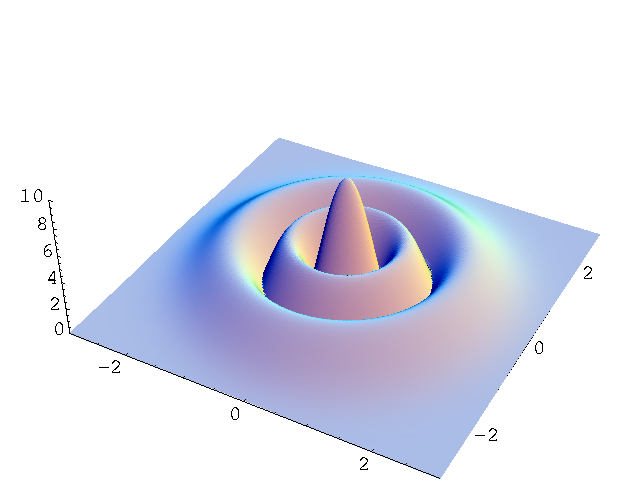
\includegraphics{GMS33.eps}
       \end{center}}
 \item \parbox[t]{130mm}{$B2sE>BP>N$G$J$$%=%j%H%s2r(BI\\
       \begin{center}
	$\begin{pmatrix}
	  0 & 0 & 1 & \cdots \\
	  0 & 0 & 0 & \cdots \\
	  1 & 0 & 0 & \cdots \\
	  \vdots & \vdots & \vdots & \ddots
	 \end{pmatrix}=$\\
	 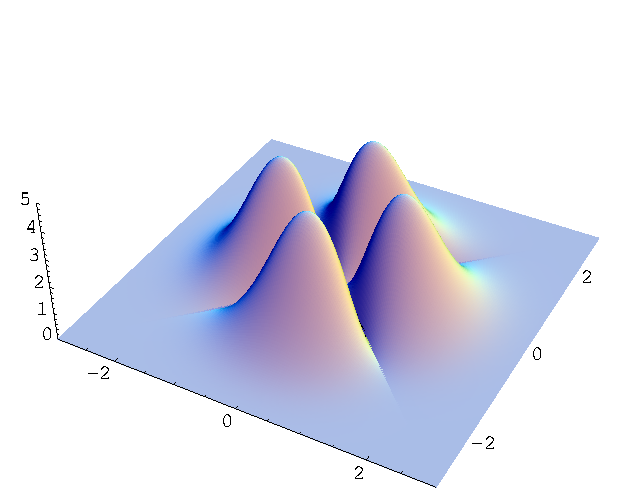
\includegraphics{GMS20.eps}
       \end{center}}
 \item \parbox[t]{130mm}{$B2sE>BP>N$G$J$$%=%j%H%s2r(BII\\
       \begin{center}
	$\begin{pmatrix}
	  0 & 0 & 0 & 0 & \cdots \\
	  0 & 0 & 0 & 0 & \cdots \\
	  0 & 0 & 0 & i & \cdots \\
	  0 & 0 & -i & 0 & \cdots \\
	  \vdots & \vdots & \vdots & \vdots &\ddots
	 \end{pmatrix}=$\\
	 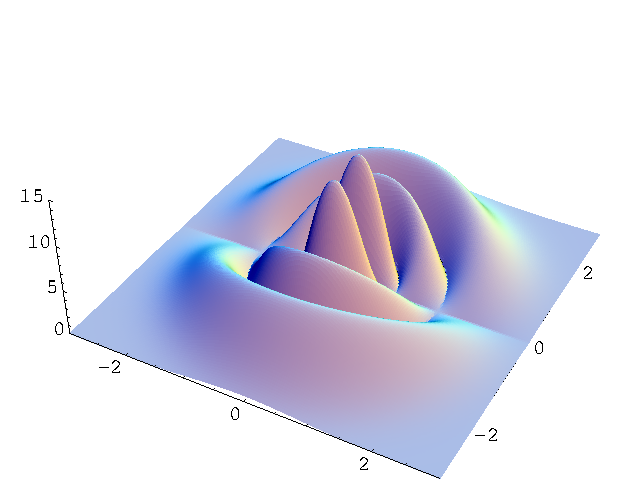
\includegraphics{GMS23I.eps}
       \end{center}}
\end{enumerate}


\subsubsection{$B9b<!85$X$N3HD%(B}

$B$3$l$^$G$O(B2$B<!85%f!<%/%j%C%I6u4V$N>l9g$r9M$($F$-$?$,!"$=$l$r(B$d+1$$B<!85(B
($+1$$B$O;~4V(B)$B$N>l9g$K3HD%$9$k!#$?$@$7;~4VJ}8~$OHs2D49@-$K4^$^$l$J$$$H$9$k!#(B
$B>l$NM}O@$G;~4VJ}8~$KHs2D49@-$rF~$l$?>l9g!"$=$N3HD%$O4JC1$G$"$k!#(B

$B$^$:!"(B$\theta^{\mu\nu}$$B$OH?BP>N9TNs$G$"$k$,!"E,Ev$J:BI8$ND>8rJQ49$K$h$C$F(B
\begin{equation}
 \theta^{\mu\nu}=
 \begin{pmatrix}
  \AntiSymBlock{\theta_1}& \zero & \cdots & \zero \\
  \zero & \AntiSymBlock{\theta_2}& \ddots & \vdots \\ 
  \vdots & \ddots & \ddots & \zero \\
  \zero & \cdots & \zero & \AntiSymBlock{\theta_{[d/2]}}\\
 \end{pmatrix}
\end{equation}
$B$H$J$k$h$&$K$9$k$3$H$,$G$-$k!#$9$k$H(B2$B<!85$N>l9g$K5"Ce$5$;$k$3$H$,$G$-$k!#(B
$B$3$&$7$FF@$i$l$?%=%j%H%s2r$O!"$?$@$N%=%j%H%s2r$+<+L@$J2r(B
($\phi(x)=\lambda_i$)$B$N@Q$K$J$C$F$$$k!#(B

\subsubsection{$B2r$N0BDj@-(B}

$B%=%j%H%s2r$rF@$k$3$H$O$G$-$?$,!"$3$l$i$N%=%j%H%s$,0BDj$J$b$N$H$7$FB8:_$7$F(B
$B$$$k$+$I$&$+$O<+L@$G$O$J$$!#$=$l$r3NG'$9$k!#(B

$B:#9M$($F$$$kM}O@$O!"(B(\ref{u-infinity-sym})$B$G<($7$?$h$&$J(B$U(\infty)$$B$NBP>N(B
$B@-$r$b$C$F$$$k$N$G$=$l$rMQ$$$F!"%=%j%H%s2r$r%*%Z%l!<%?$N8@MU$G(B$\ket{n}$$B$N(B
$B4pDl$K$D$$$FBP3Q$K;}$C$F$$$/$3$H$,$G$-$k!#$=$N$H$-$N2r$O!"(B
\begin{equation}
 \label{radial-solution}
 \begin{pmatrix}
  a_1 & 0 & \cdots & \cdots & \cdots & \cdots & 0 \\
  0 & a_2 & \ddots & \ddots & \ddots & \ddots & \vdots \\
  \vdots & \ddots & \ddots &\ddots &\ddots & \ddots & \vdots \\
  \vdots & \ddots & \ddots & a_n & \ddots & \ddots & \vdots \\
  \vdots & \ddots & \ddots &\ddots & 0 &  \ddots &\vdots \\
  \vdots & \ddots & \ddots &\ddots &\ddots & \ddots & \vdots \\
  0 & \cdots & \cdots & \cdots & \cdots & \cdots & 0 \\
 \end{pmatrix}
\end{equation}
$B$N$h$&$J7A$K$J$C$F$$$k!#C"$7!"(B$a_n$$B$O@h$K=R$Y$?$h$&$K!"%]%F%s%7%c%k(B$V$$B$NDd(B
$BN1E@(B$\lambda_i$$B$KCM$r$H$k!#$3$N2r$N%(%M%k%.!<$O(B
\begin{eqnarray}
 E &=& {2\pi\theta\over g^2}\Tr V(\phi) \nonumber \\
   &=& {2\pi\theta\over g^2}\sum^\infty_{n=0}V(a_n)
\end{eqnarray}
$B$H$J$k!#$7$?$,$C$F!"(B$a_n$$B$,%]%F%s%7%c%k(B$V$$B$N6K>.CM$G$"$l$P!"@]F0O@E*$K$O0B(B
$BDj$G$"$k$3$H$,J,$+$k!#(B

$B99$K!"(B$\theta\rightarrow\infty$$B$N6K8B$G$O!">l$N%(%M%k%.!<$,(B$\theta$$B$KHfNc(B
$B$7$F$$$k$N$G!"%]%F%s%7%c%k$NB>$N6K>.CM$dIi$NL58BBg$X$N%H%s%M%k$OM^@)$5$l$k(B
$B$N$GHs@]F0O@E*$K$b0BDj$G$"$k!#(B

\subsubsection{$\theta$$B$,M-8B$N;~$N(BGMS$B%=%j%H%s(B}

GMS$B%=%j%H%s$OHs2D49>l$NM}O@FCM-$NBP>]$G$"$k!#$7$?$,$C$F!"(B$\theta$$B$rM-8B$K(B
$B$7$F$=$N@dBPCM$r(B$0$$B$K$9$k$H(BGMS$B%=%j%H%s$OL5$/$J$C$F$7$^$&$3$H$,M=A[$5$l$k!#(B
$B$=$l$O;v<B$G$"$j!"<B:]$K$O(B$\theta$$B$N8:>/$KH<$J$C$F(BGMS$B%=%j%H%s2r$,L5$/$J$C(B
$B$F$7$^$&$3$H$,J,$+$k!#(B\cite{NCSolFinTheta}

$\theta$$B$,M-8B$N;~$O!"1?F09`$r9M$($J$/$F$O$J$i$J$$!#$^$:!"HyJ,$O:BI8$N%j(B
$B%9%1!<%k$N8e!"(B
\begin{equation}
 \left\{
  \begin{array}{l}
   \partial_x\rightarrow i[\yh,\cdot]
    ={1\over\sqrt{2}}[\anih -\crea,\cdot]\\
   \partial_y\rightarrow -i[\xh,\cdot]
    =-i{1\over\sqrt{2}}[\anih +\crea ,\cdot]\\
  \end{array}
 \right.
\end{equation}
$B$H=q$/$3$H$,$G$-$k!#$9$k$H!"(B
\begin{equation}
 \int dxdy\, \1half\left(\partial_x\phi^2+\partial_y\phi^2\right)
  =\pi \Tr ([\crea,\hat{\phi}][\anih,\hat{\phi}])
\end{equation}
$B$H$3$m$G!"$3$N1?F09`$O(B$\crea$$B$d(B$\anih$$B$r4^$s$G$$$k$N$G!"@h$K=R$Y$?(B
$U(\infty)$$B$NBP>N@-$r2u$7$F$7$^$&!#$h$C$F!"2sE>BP>N$J2r$K>o$K;}$C$F$$$1$k(B
$B$H$O8B$i$J$$$,!"$3$3$G$O2sE>BP>N$J(B\ref{GMSradial-solution}$B$N$h$&$J2r$N$_$r(B
$B9M$($k!#$9$k$H!"%*%Z%l!<%?$N8@MU$G=q$+$l$?%O%_%k%H%K%"%s$O!"(B
\begin{equation}
 \Ham =\sum_{n=0}^\infty {1\over 4}
  [(2n+1)a_n^2-2(n+1)a_na_{n+1}]+\theta V(a_n)
\end{equation}
$B$H$J$k!#8EE5E*$J2r$O(B
\begin{equation}
 {\partial\Ham\over\partial a_n}=0
\end{equation}
$B$K$h$C$FF@$k$3$H$,$G$-$k!#$3$l$O!"(B
\begin{equation}
 \left\{
  \begin{array}{ll}
   (n+1)a_n-(2n+1)+na_{n-1}=2\theta V'(a_n)\hspace{5mm}& (n\geq1) \\
   a_1-a_0=2\theta V'(a_0)\hspace{5mm}& (n=0\hbox{$B$KBP1~(B}) \\
  \end{array}
\right.
\end{equation}
$B$H$$$&L58B8D$N:9J,J}Dx<0$K$J$k!#3F<0$r(B$N$$B$^$GB-$79g$o$;$k$H!"(B$\theta$$BM-(B
$B8B$N;~$N2sE>BP>N$J%=%j%H%s2r$N%*%Z%l!<%?!<$K$h$kI=8=$NBP3Q@.J,(B
$a_n$$B$NK~$?$9$Y$-<0$N:G=*7A$O!"(B
\begin{equation}
 \label{finite-theta-equation}
 a_{N+1}-a_N={2\theta\over N+1}\sum^N_{n=0} V'(a_n)
\end{equation}
$B$H$$$&<0$K$J$k!#99$K!"%(%M%k%.!<$,M-8B$G$"$k$3$H$rMW5a$9$k$H!"(B
\begin{equation}
 \label{finite-theta-convergence-condition}
 \left\{
 \begin{array}{l}
  a_n\rightarrow0\quad(n\rightarrow\infty)\\
  \sum\limits_{n=0}^\infty V'(a_n)<\infty \\
 \end{array}\right.
\end{equation}
$B$H$$$&I,MW>r7o$,$G$k!#(B

$B$3$3$G!"(B$\theta$$B$r(B$0$$B$K6a$E$1$k$3$H$r9M$($F$_$k!#(BGMS$B%=%j%H%s$O;~6u$NHs2D(B
$B49@-$,$"$C$F;O$a$FB8:_$9$k$b$N$G$"$k$3$H$+$i!"(B$\theta\rightarrow 0$$B$G(BGMS 
$B%=%j%H%s$O>C$($F$7$^$&$O$:$G$"$k!#@_Dj$H$7$F!"(B$T=0$$B$r??$N??6u$K$H$C$F9M(B
$B$($k!#(B(\ref{finite-theta-equation})$B$r8+$k$H!"(B$\theta$$B$O(B$a_n$$B$,F0$/I}$r5,(B
$BDj$7$F$$$k$3$H$,J,$+$k!#(B$\theta$$B$,==J,>.$5$$;~$O!"(B$a_n$ $B$NJQ2=$,Hs>o$K>.(B
$B$5$$$N$G<0(B(\ref{finite-theta-equation})$B$N1&JU$O@QJ,$H$7$FNI$$6a;w$K$J$k!#(B
$BB($A!"(B
\begin{align}
 a_{n+1}-a_n\simeq 2\theta\int^{a_n}_{a_0}da\, V'(x)&=2\theta(V(a_n)-V(a_0))
  \nonumber\\
 &\xrightarrow{n\rightarrow\infty}-2\theta V(a_0)
\end{align}
$B$H$J$k!#$h$C$F!"(B(\ref{finite-theta-convergence-condition})$B$rK~$?$90Y$K$O!"(B
$V(a_0)=0$$BB($A(B$a_0=0$$B$G$J$/$F$O$J$i$J$$!#$7$+$7!"$3$N=i4|>r7o$G:9J,(B
$BJ}Dx<0(B(\ref{finite-theta-equation})$B$r2r$/$H!"<+L@$J2r$7$+M?$($J$$!#$h$C(B
$B$F!"(B$\theta$$B$,==J,>.$5$/$F!":9J,J}Dx<0(B(\ref{finite-theta-equation})$B$N1&(B
$BJU$NOB$r@QJ,$H$7$F8+$k$3$H$,$G$-$k$H$-$O!"<+L@$J2r$7$+L5$$$3$H$,J,$+$C$?!#(B

$B$3$l0J>e$N5DO@$r?J$a$k$?$a$K$O6qBNE*$K%]%F%s%7%c%k$N7A$rM?$($F?tCME*$J7W(B
$B;;$r9T$J$o$J$/$F$J$J$i$J$$!#%]%F%s%7%c%k$N7A$rM?$($F?tCME*$K2r@O$7$?5DO@(B
$B$O(B\cite{NCSolFinTheta}$B$G$J$5$l$F$$$k!#(B

\subsubsection{$\theta$$B$,M-8B$G%2!<%8>l$,$"$k;~(B}

$B>e$G8+$?$h$&$K!"%9%+%i!<>l$@$1$N;~$K$O(B$\theta$$BM-8B$GHs<+L@$J2r$r9=@.$7$h(B
$B$&$H$7$F$b7k6I:9J,J}Dx<0$K5"Ce$9$k$N$_$@$,!"%2!<%8>l$,B8:_$9$k;~$K$O1?F0(B
$B9`$,F~$C$F$$$F$b(B$U(\infty)$$B$NBP>N@-$,2sI|$9$k(B\footnote{$U( \infty)$$B$NL5(B
$B8B>.JQ49(B$1+\lambda$($\lambda$:Hermite)$B$KBP$7$F(B$A_\mu \rightarrow A+
\partial_\mu\lambda$$B$H$9$l$P$h$$!#(B}$B$N$G!"2r@OE*$J87L)2r$r9=@.$9$k$3$H$,(B
$B$G$-$k!#(B

$B$^$:!"6qBNE*$J2r$r5a$a$kA0$K%*%Z%l!<%?!<7A<0$G(B$U(\infty)$$BBP>N@-$,B8:_$9(B
$B$k;~$K%=%j%H%s2r$r9=@.$9$k0lHLE*$JJ}K!(B\cite{ExactNCSol}$B$K$D$$$F@bL@$9$k!#(B

$B:#!"(BHilbert$B6u4V$K:nMQ$9$k1i;;;R(B$U$$B$r9M$($k$H!"(B$U$$B$N:nMQ$O(B
\begin{equation}
 \begin{split}
  \ket{\psi}\rightarrow U\ket{\psi} \\
  \bra{\psi}\rightarrow \bra{\psi}\Ud \\
  \OpO\rightarrow U\OpO\Ud
 \end{split}
\end{equation}
$B$H$J$k!#$b$7(B$U$$B$,(Bisometry$B$G$"$kB($A(B
\begin{equation}
 \label{isometry}
  U\Ud=1
\end{equation}
$B$rK~$?$7!"$7$+$7$J$,$i%f%K%?%j$G$O$J$i$P!"JQ49(B$U$$B$K$h$C$F1?F0J}Dx<0$N2r(B
$B$OJL$N2r$X$HJQ49$5$l$k!#(B($U$$B$,%f%K%?%j$J$i$PK\<AE*$KF1$82r$X$HJQ49$5$l$k!#(B)
$B2?8N$J$i$P!"J*M}E*<+M3EY$rI=$o$91i;;;REy$r4^$`0lHL$N1i;;;R$KBP$7$F(B
\begin{equation}
 \frac{\delta S}{\delta \OpO}\rightarrow
  U\frac{\delta S}{\delta \OpO}\Ud
\end{equation}
$B$H$J$k$+$i!"7PO)@QJ,$N6KCM$rM?$($k$h$&$JG[0L$rJL$N7PO)@QJ,$N6KCM$rM?$($k(B
$B$h$&$JG[0L$KJQ49$9$k$+$i$G$"$k!#$3$N$h$&$JJQ49(B$U$$B$r(Bsolution generating
transformation $B$H$$$&!#(B

$B$3$3$G!"(BHilbert$B6u4V$H$7$F(B1$B8D$ND4OB?6F0;R$,@.$9(BFock$B6u4V$r9M$($k!#(Bshift
operator$S$$B!"(B
\begin{equation}
 \label{shift-operator}
 S\equiv\sum^\infty_{k=o}\ket{k+1}\bra{k}
\end{equation}
$B$O!"(B
\begin{equation}
 \Sd^nS^n=1,\quad S^n\Sd^n=1-P_n
\end{equation}
$B$H$$$&4X78$rK~$?$9!#C"$7!"(B
\begin{equation}
 P_n=\sum^{n-1}_{k=0}\ket{k}\bra{k}
\end{equation}
$B$G$"$k!#(B$S^n$$B$O<0(B(\ref{isometry})$B$rK~$?$9$N$G(Bsolution generation
transformation$B$G$"$k!#:#(B$S^n\Sd^n$$B$O(BHilbert$B6u4V$N(B$\ket{0}\sim\ket{n-1}$ 
$B$K1w$$$F$N$_%f%K%?%jJQ49$G$J$$!#(B$\ket{n}$$B$OH>7B(B$\sqrt{n\theta}$$B$NNN0h$K(B
$BBP1~$7$F$$$?$+$i!"2r@8@.JQ49(B$S^n$$B$K$h$C$F!"H>7B(B$\sqrt{n\theta}$$B$NHs2D49(B
$B%=%j%H%s$r:n$k$3$H$,$G$-$k$H9M$($k$3$H$,$G$-$k!#(B

$B6qBNE*$J7W;;$K0\$k$H!":#9M$($k:nMQ$O(B
\begin{equation}
 \int dxdy\, \left(\1half(F_{xy})^2
	      +\1half D^\mu\phi D_\mu\phi -V(\phi)\right)
\end{equation}
$B$G$"$k!#$3$l$r:BI8$N%j%9%1!<%k$N8e$K!"%*%Z%l!<%?!<$N8@MU$K=q$-D>$9!#JX59(B
$B$N0Y!"%2!<%8>l$O<!$N$h$&$KI=5-$9$k$3$H$K$9$k!#(B
\begin{equation}
 A\equiv A_z=-\frac{i}{\sqrt{2}}(A_x-iA_y),\quad
  \Ab\equiv A_{\zb}=-\frac{i}{\sqrt{2}}(A_x+iA_y)
\end{equation}
$B<!$K6&JQHyJ,$r%*%Z%l!<%?!<$N8@MU$G=q$/$3$H$r9M$($k(B
\begin{equation}
 \creC\equiv \anih+i\theta^{\1half}A,\quad
  \aniC\equiv \crea-i\theta^{\1half}\Ab
\end{equation}
$B$H$9$k$H!"(B
\begin{eqnarray}
 \frac{1}{\sqrt{2}}[D_x-iD_y,\phi]=-[\aniC,\phi]
 \frac{1}{\sqrt{2}}[D_x+iD_y,\phi]=[\creC,\phi]
\end{eqnarray}
$B$3$N6&JQHyJ,$r;H$C$F(Bfield strength$B$O%*%Z%l!<%?!<$N8@MU$G<!$N$h$&$K=q$1$k!#(B
\begin{equation}
 F\equiv -F_{xy}=-i[\crea,\Ab]-i[\anih,A]+\theta^{\1half}[A,\Ab]
  =\theta^{-\1half}([\aniC,\creC]+1)
\end{equation}
$B7k6I!"%*%Z%l!<%?!<7A<0$G=q$+$l$?%O%_%k%H%K%"%s$O(B
\begin{equation}
 \Ham=2\pi\Tr\left(\1half([\aniC,\creC]+1)^2
		 +[\aniC,\phi][\creC,\phi]
		 +\theta V(\phi)\right)
\end{equation}
$B$H$J$k!#$3$N7O$N<+L@$J2r$O(B$\phi_*$$B$r(B$V(\phi)$$B$N6K>.CM$rM?$($k(B$\phi$$B$NCM(B
$B$H$7!"99$K(B$V(\phi_*)=0$$B$9$l$P!"(B
\begin{equation}
 \begin{split}
  \phi&=\phi_*\\
  A&=0\Rightarrow \creC=\anih,\,\aniC=\crea
 \end{split}
\end{equation}
$B$G$"$k!#$3$l$r@h$N(Bsolution generating transformation$B$K$h$C$FJL$N2r$K<L$9$H!"(B
\begin{equation}
 \begin{split}
  \phi&=\phi_*(1-P_n) \\
  \creC&=S^n\anih\Sd^n,\,\aniC=S^n\crea\Sd^n
 \end{split}
\end{equation}
$B$H$J$k!#$3$l$OHs<+L@$J2r$G$"$k!#$3$N;~(Bfield strength$B$O!"(B
\begin{equation}
 F=\theta^{-\1half}([\creC,\aniC]-1)=\theta^{-\1half}(S^n\Sd^n-1)
  =\theta^{-\1half}P_n
\end{equation}
$B$G$"$j!"(B$[\creC,S^n\Sd^n]=0$$B$H$J$k$+$i!"$3$N2r$N;}$D%(%M%k%.!<$O(B
\begin{equation}
 E=2\pi n\left(\frac{1}{2\theta}+\theta V(0)\right)
\end{equation}
$B$H$J$k!#(B

 %#!platex master.tex

\subsection{D-brane$B$H(BGMS$B%=%j%H%s(B} 
\label{d-brane-and-soliton}
D-brane$B$d(BF-string$B$O:GBg8B$KHs2D49@-$rF~$l$?6K8BB($A!"(B
$B\rightarrow\infty$$B$N6K8B$G(BGMS$B%=%j%H%s$K4X78$7$F$$$k(B\footnote{$BHs2D49@-$r(B
$BF~$l$J$/$F$b%?%-%*%s>l$N%=%j%H%s2r$,(BDp-brane$B$H4X78$7$F$$$k$i$7$$>Z5r$b$$$/(B
$B$D$+$"$k(B\cite{DbraneLumpOSFT}\cite{LumpBraneOSFT}$B!#(B}$B$i$7$$>Z5r$,$$$/$D$+$"(B
$B$k(B\cite{DbraneStNCsol}$B!#$3$3$G$O$=$N>Z5r$r$$$/$D$+<($9!#(B

\subsubsection{D-brane$B$N%F%s%7%g%s(B}
$B$^$:!"(BDp-brane$B$N%F%s%7%g%s(B$T_p$$B$H(BD(p-1)-brane$B$N%F%s%7%g%s$N4X78$r5a$a$k!#(B
$B$^$:!"H>7B(B$R_1,\ldots,R_p$$B$N(Bp-$B%H!<%i%9$K4,$-$D$$$?(BD-brane$B$r9M$($k!#$9$k$H!"(B
$B$=$N<ANL$O(B
\begin{equation}
 T_p\E^{-\Phi}\prod^p_{i=0}2\pi R_i
\end{equation}
$B$?$@$7!"(B$\Phi$$B$O%G%#%i%H%s>l$G$"$k!#(Bp-$BJ}8~$N(BT-dual$B$r<h$k$H!"<ANL$OJQ2=$7$J(B
$B$$$,%G%#%i%H%s>l$,Hs<+L@$JJQ49(B
\begin{equation}
 \E^{\Phi'}={\ap^{1/2}\over R}\E^{\Phi}
\end{equation}
$B$G7k$P$l$F$$$F!"$^$?(Bp-$BJ}8~$NBN@Q@QJ,$,8:$k$N$G!"(B
\begin{equation}
 2\pi\ap^{1/2}T_p\E^{-\Phi'}\prod^{p-1}_{i=1}2\pi R_i
\end{equation}
$B$H=q$1$k!#$h$C$F(B
\begin{equation}
 T_{p-1}=2\pi \ap^{1/2} T_p
\end{equation}
$B$G$"$k!#$h$C$F!"(BDp-brane$B$N%F%s%7%g%s$O(B
\begin{equation}
 \label{Dbrane-tension}
 T_p=(2\pi \ap)^{25-p\over 2} T_{25}
\end{equation}

\begin{figure}[th]
 \begin{center}
  \input{exchange.pstex_t}
  \caption{$B3+89$N@8@.>CLG(B}
  \label{crea-anih}
 \end{center}
\end{figure}

$B<!$K!"%F%s%7%g%s$N6qBNE*$JCM$r7W;;$9$k!#$3$N7W;;$O!"?^(B\ref{crea-anih}$B89(B
$BM}O@$K$h$k(Btree-level$B$G$N7W;;$G$N%0%i%S%H%s$N8r49$N?6I}$H!"89M}O@$NDc%(%M(B
$B%k%.!<M-8zM}O@$G$"$k=ENO>l$NM}O@$H(BDirac-Born-Inferd($B%F%s%7%g%s$r%Q%i%a!<(B
$B%?$H$7$F4^$`(B)$B$rAH$_9g$o$;$?>l$NM}O@(B\ref{crea-anih}$B$KBP1~$9$k$h$&$J%0%i%S(B
$B%H%s$N8r49$N?6I}$r8=$o$9%W%m%Q%2!<%?!<$rHf3S$9$k$3$H$G$J$5$l$k!#7W;;$N>\(B
$B:Y$r=R$Y$k$HD9$/$J$k$N$G!">\:Y$O(BPolchinski$B$N652J=q(B
\cite[p273$\sim$p277]{PolchinskiST}$B$KG$$;$k!#(B

$B$3$N7W;;$K$h$jF@$i$l$?2r$O!"(B
\begin{equation}
 T_p\E^{-\Phi}={\sqrt{\pi}\over 8 \kappa}(4\pi\ap)^{11-p\over 2}
  \hspace{1cm}\left(\kappa =2\pi \E^{\Phi}\right)
\end{equation}
$B$H$J$k!#(B

\subsubsection{$B%?%-%*%s>l$N%=%j%H%s$N<ANL(B}
\begin{figure}[ht]
 \begin{center}
  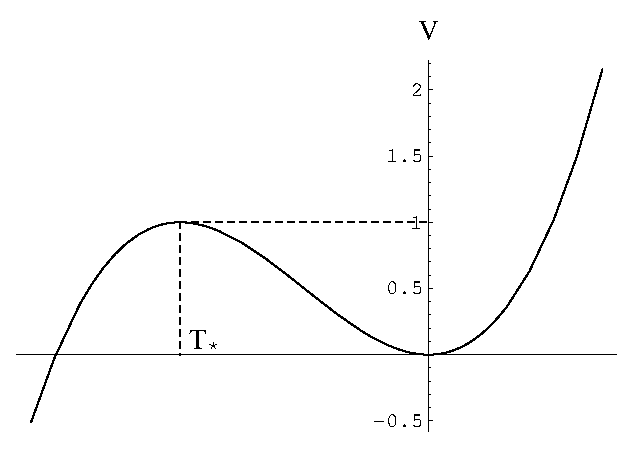
\includegraphics{tachyon-potential.eps}
  \caption{$B%?%-%*%s>l$N%]%F%s%7%c%k(B}
  \label{tachyon-potential}
 \end{center}
\end{figure}

$B<!$K%?%-%*%s>l$N%=%j%H%s$N<ANL$r5a$a$k!#%?%-%*%s>l$N:nMQ$r5a$a$k$KEv$?$j!"(B
String Field Theory $B$+$iM=A[$5$l$F$$$k2>@b(B($B>\:Y$O(B
\cite{DescentRelBosDbrane}\cite{DbraneLumpOSFT}\cite{TacCondSSFT})$B$K$D$$(B
$B$F$N@bL@$r$7$J$/$F$O$J$i$J$$!#(Bbosonic$B$J89M}O@$G$N(BD25-brane$B$O%?%-%*%s>l$r(B
$B;}$C$F$$$k$,!"$=$N%]%F%s%7%c%k$O?^(B\ref{tachyon-potential}$B$N$h$&$J7A$r$7(B
$B$F$*$j(B($BC"$7!"$3$3$G%]%F%s%7%c%k$O(B$T=T_\ast$$B$N;~(B$V(T_\ast)=1$$B$K$J$k$h$&$K(B
$B@55,2=$7$F$"$k!#(B)$B!"(BD25-brane$B$,$"$k??6u$O!"?^(B\ref{tachyon-potential} $B$N(B
$T=T_\ast$$B$NE@$KBP1~$7$F$$$k!#%?%-%*%s$,6E=L$9$k$3$H$K$h$C$F!"(B$T=0$$B$N(B
D25-brane$B$NL5$$(Bopen string vacuum$B$K9T$/$H?.$8$i$l$F$$$k!#(B

$B$$B>l$,F~$l!"=E$$>l$r@QJ,$7$F!"F@$i$l$k%?%-%*%s>l$NM-8z:nMQ$O(B
\begin{equation}
 S=-{T_{25}g_s\over G_s}\int d^{26}\, \sqrt{G}\left(
  \1half f(T)G^{\mu\nu}\partial_\mu T \partial_\nu T + \cdots
  -V(T) \right)
\end{equation}
$BC"$7(B$G_s,G^{\mu\nu}$$B$O(B(\ref{openstring-parameters})$B$GDj5A$7$?(Bopen string 
$B$N%a%H%j%C%/$H%+%C%W%j%s%0$G$"$k!#99$K!"(BGMS$B%=%j%H%s2r$rF3=P$9$k:]$K9T$J$C(B
$B$?$h$&$K(B$B\rightarrow\infty$$B$N6K8B$r<h$j!"(B
$x_{24}\rightarrow\sqrt{\theta}x_{24},x_{25}\rightarrow\sqrt{\theta}x_{25}$ 
$B$H@QJ,JQ?t$N%j%9%1!<%k$r9T$$(B$x_{24},x_{25}$$B@QJ,$r%*%Z%l!<%?7A<0$N%H%l!<(B
$B%9$K=q$-49$($F!"%O%_%k%H%K%"%s$rF@$k$H!"(B
\begin{equation}
 \Ham ={2\pi T_{25}g_s\theta\over G_s}\int d^{24}x\, \sqrt{G}
  \sum_{n=0}^\infty V(a_n) \hspace{1cm}(a_n\in\{0,T_\ast\})
\end{equation}
$B$H$J$k!#(B

$B$3$3$G<0(B(\ref{GMSradial-solution})$B$N(B$a_0=T_\ast,a_n=0(n\geq 1)$$B$J$k2r$r9M(B
$B$($k$H!"(B
\begin{equation}
 \Ham=(2\pi)^2\ap T_{25} \int d^{24}x\, \sqrt{g}=T_{23}\int d^{24}x\sqrt{g}
\end{equation}
$B$H$J$j!"%F%s%7%g%s$O(BD23-brane$B$N$=$l$H0lCW$9$k!#$5$i$K!"<0(B
($\ref{GMSradial-solution}$)$B$G(B$a_0,a_1,\ldots,a_k=T_\ast,\quad
a_{k+1} , \ldots = 0$$B$J$k2r$r9M$($k$H!"$=$N%F%s%7%g%s$O(Bk$BKg$N(BD23-brane$B$N%F%s(B
$B%7%g%s$K0lCW$9$k(B

$B$3$N7W;;$OG$0U$N6v?t<!85$N(BD-brane$B$N%F%s%7%g%s$K3HD%$G$-$k$3$H$b<+L@$G$"$k!#(B

$B0J>e$N;v<B$+$i!"IT0BDj$J(BD-brane$B$N>e$N%?%-%*%s>l$,(BGMS$B%=%j%H%s$H$7$F$NG[0L(B
$B$r;}$D$H$-$K$O!"(BD25-brane$B$,(Bclosed string vacuum$B$K9T$/$HF1;~$K(B
D$(25-2n)$-brane$B$,;D$k$H$$$&$3$H$,?dB,$5$l$k!#(B

\subsubsection{$B%2!<%8>l$X$N%+%C%W%j%s%0(B}

GMS$B%=%j%H%s$r(BD-brane$B$HF1Dj$9$k0Y$K$O!"%2!<%8>l$X$N%+%C%W%j%s%0$,(BD-brane 
$B$HF1$8$G$"$k$3$H$r<($5$J$/$F$O$J$i$J$$!#(B

$B$^$:$O!"(BD-brane$B>e$N%2!<%8>l$H%?%-%*%s>l$r4^$`:nMQ$r=q$-2<$5$J$/$F$O$J$i(B
$B$J$$$,!":#9M$($F$$$kM}O@$OHs2D496u4V>e$G$NM}O@$G$"$k$+$i!"%2!<%8M}O@$NIt(B
$BJ,$OHs2D49%2!<%8M}O@$K$J$C$F$$$k!#$9$J$o$A%2!<%8JQ49$O!"(B
\begin{equation}
 \delta_\lambda A_\mu=\partial_\mu\lambda-i[A_\mu,\lambda]_\star
\end{equation}
$B$H$J$C$F$$$F!#(BField Strength$B$O(B
\begin{equation}
 F_{\mu\nu}=\partial_\mu A_\nu -\partial_\nu A_\mu -i[A_\mu,A_\nu]_\star
\end{equation}
$B$H=q$+$l$k!#$3$3$G!"%?%-%*%s>l$OHs2D49%2!<%8JQ49$K$h$C$F(Badjoint$B$KJQ49$9(B
$B$k!#B($A!"(B
\begin{equation}
 \delta_\lambda T=-i[t,\lambda]_\star
\end{equation}
$B$H$J$k!#(B

$B%2!<%8>l$H%?%-%*%s>l$N:nMQ$O<!$N$h$&$J7A$r$7$F$$$k!#(B
\begin{equation}
 S={g_s T_{25}\over G_s}\int d^{26}\sqrt{G}\left(\1half f(T)D^\mu TD_\mu T 
	-V(T) -{1\over 4}h(T)F^{\mu\nu}F_{\mu\nu}\right)
\end{equation}
$B$3$l$rHs2D49$J(B2$B<!85$NJ}8~$H2D49$J(B24$B<!85$NJ}8~$KJ,2r$9$k!#$3$3$G!"(BGMS$B%=%j(B
$B%H%s$NF3=P$N;~$HF1$8%;%C%H%"%C%W$r9M$($k$N$G!"Hs2D49J}8~$NHyJ,$OL5;k$7$F(B
$B$h$$!#Hs2D49J}8~$N:BI8$r(B$i,j$$B$=$l0J30$N:BI8$r(B$a,b,\ldots$$B$9$k$H!"(B
\begin{eqnarray}
 S={g_s T_{25}\over G_s}\int d^{26}\sqrt{G}(\1half f(T)D^a T D_a T 
  -\1half h(T)D^a A_i D_a A^i -V(T)
  -\1half f(T)[A_i,T]_\star [A^i,T]_\star \nonumber \\
 +{1\over 4}h(T)[A_i,A_j]_\star [A^i,A^j]_\star -{1\over 4}h(T)F^{ab}F_{ab})
\end{eqnarray}
$B$H$J$k!#$b$O$d!"(B$A_i$$B$O%9%+%i!<N3;R$G$"$j!"(Badjoint$B$N%2!<%8JQ49@-$r;}$C$F(B
$B$$$k!#(B

$B:#!"Hs2D49J}8~$K(BGMS$B%=%j%H%s2r(B$T=T_*\phi_0$$B$+$i$N%U%i%/%A%e%(!<%7%g%s$r9M(B
$B$(!"Hs2D49J}8~$NM}O@$r%*%Z%l!<%?!<7A<0$K=q$-D>$9!#B($A!"(B
\begin{align}
 T&=T_*\phi_{00}+\sum^\infty_{m,n=0}T^{mn}\phi_{mn}\\
 A_a(x^\mu)&=\sum^\infty_{m,n=0}A^{mn}_a(x^b)\phi_{mn} \\
 A_i(x^\mu)&=\sum^\infty_{m,n=0}A^{mn}_i(x^b)\phi_{mn}
\end{align}
$B$3$3$G!"(B$\phi_{mn}$$B$O(B
$B$9$k$H!"(B$\phi_{00}$$B$K$+$+$kItJ,$9$J$o$A(BD7-brane$B$K4X$o$kItJ,$@$1$rH4$-=P$9(B
$B$H(B(00$B$NB-$OJX59$N0Y$K>JN,$9$k!#(B)$B!"(B
\begin{equation}
 S=T_23\int d^{24}x \sqrt{g}\left(\1half
	f(T_*)\partial^a\delta T\partial_a\delta T
	-V(T_*+\delta T)
	+\1halfh(T_*)\partial^aA_i\partial^aA^i 
	-{1\over 4}h(T_*)F^{ab}F_{ab}\right)
\end{equation}
$B$3$l$O@5$K(BD23-brane$B$N%?%-%*%s$H(Bbrane$B$K?bD>J}8~$N:BI8$NNO3X$r5-=R$9$k:nMQ(B
$B$K$J$C$F$$$k!#(B


\subsection{D-brane$B%A%c!<%8$H(BK-theory}
\nocite{TopoChargeNCSol}

\ref{differential}$B@a$G8+$?$h$&$K!"(BK-theory$B$OHs2D494v2?3X$K$*$$$F0lHL$N4v(B
$B2?3X$N%3%[%b%m%8!<$NLr3d$r2L$?$7$F$$$k!#(BD-brane$B%A%c!<%8$H(BK-theory$B$N4X78(B
$B$O!"89M}O@$NK\<A$,Hs2D494v2?3X$G$"$k$3$H$N>u67>Z5r$H8+$k$3$H$,$G$-$k!#$3(B
$B$3$G$O!"(BD-brane$B%A%c!<%8$H(BK-theory$B$N4X78$K$D$$$F@bL@$9$k!#(B

\subsubsection{$BJ,N`6u4V$HHs2D49%=%j%H%s(B}

$B:#!"(BDp-brane$B$,B?MMBN(B$X\times \Real^{2n}$$B$K4,$-$D$$$F$$$k$H9M$($k!#A0$N;h(B
$B@a$G(B$\Real^{2n}$$BJ}8~$X$N%?%-%*%s$N(BGMS$B%=%j%H%s2r$,(BD$(p-2n)$-brane$B$KBP1~$7(B
$B$F$$$k$3$H$r@bL@$7$?!#:#!"Hs2D496u4V>e$N4X?t$N$J$9(B$\Cst$$B4D$O(B$n$$B8D$ND4OB(B
$B?6F0;R$N@.$9(BFock$B6u4V$K:nMQ$9$k:nMQAG$N@.$94D(B$\AlgB$$B$H8+Jo$9$3$H$,$G$-$?!#(B
$B$9$k$H!"$3$N(BDp-brane$B$N>e$N4X?t$N@.$94D(B$C_0(X\times\Real^{2n})$$B$N85$G$"$k(B
$B%?%-%*%s>l$O!"(B$C_0(X\times\Real^{2n})=C^\infty(X)\otimes\AlgB$$B$G$"$k$+$i!"(B
$B$3$N(BDp-brane $B>e$N4X?t(B$T$$B$O(B
\begin{equation}
 T:X\rightarrow\AlgB
\end{equation}
$B$H$$$&B?MMBN(B$X$$B$+$i(B$\AlgB$$B$X$N<LA|$N@.$9O"B3<LA|$G$"$k$H8+$k$3$H$,$G$-$k!#(B
$BC"$7O"B3$H$O!"(B$\AlgB$$B$N(Bnorm$B%H%]%m%8!<$K$h$C$FDj5A$5$l$F$$$k!#(B
\ref{d-brane-and-soliton}$B@a$G@bL@$7$?$h$&$K!"(BGMS$B%=%j%H%s$O<M1F1i;;;R$H8+(B
$B$k$3$H$,$G$-$k!#:#!"%?%-%*%s>l(B$T$$B$N%]%F%s%7%c%k$,?^(B
\ref{tachyon-potential} $B$N7A$r$7$F$$$k$3$H$r2>Dj$9$k$H!"DdN1E@$O(B
$T=T_*,0$$B$N(B2$B$D$G$"$k$+$i!"(BGMS$B%=%j%H%s2r$O$=$N%i%s%/$K$h$C$FFCD'$E$1$k$3(B
$B$H$,$G$-$k!#(B$\Rank(n)$$B$N<M1F1i;;;R$N$J$96u4V$O(BGrassmann$BB?MMBN(B$G(n)$$B$H$7(B
$B$FCN$i$l$F$$$k!#$7$?$,$C$F!"%?%-%*%s>l$,(B$\Rank(n)$$B$N(BGMS$B%=%j%H%s$r7A@.$7(B
$B$F$$$k$H$-!"(B
\begin{equation}
 T:X\rightarrow G(n)
\end{equation}
$B$H=q$/$3$H$,$G$-$k!#(B

$B:#6=L#$r;}$C$F$$$k(BHilbert$B6u4V$OL58B<!85$G$"$k$,!"2>$KM-8B<!85$N(BHilbert$B6u(B
$B4V(B$\Cplx^k$$B$NCf$N<M1F1i;;;R$N6u4V$r9M$($k$H$=$l$O!"(B$G_k(n)=U(k)\diagup
(U(k)\times U(k-n))$$B$G$"$k!#L58B<!85$N(BHilbert$B6u4V$N(B$\Rank(n)$$B$N<M1F1i;;(B
$B;R$N@.$96u4V(B$G(n)$$B$O$3$N5"G<E*6K8B(B$\lim_{k\rightarrow\infty}G_k(n)$$B$H$7(B
$B$FDj5A$5$l$F$$$k!#(B

$B<B$O!"(BGrassmann$BB?MMBN(B$G(n)$$B$OJ#AG%Y%/%H%kB+$NJ,N`6u4V$G$"$k$3$H$,CN$i$l(B
$B$F$$$k!#J,N`6u4V$H$O0J2<$N$h$&$J@-<A$rK~$9$b$N$H$7$FDj5A$5$l$F$$$k!#(B
\begin{Def}[$BJ,N`6u4V(B]
 $B0J2<$N@-<A$rK~$?$96u4V$rJ,N`6u4V(B$BU(n)$$B$H$$$&(B
\begin{enumerate}[B1]
 \item $BG$0U$NB?MMBN(B$M$$B>e$N(B$\Rank=n$$BJ#AG%Y%/%H%kB+$N%[%b%H%T!<F1CMN`$,(B$M$
       $B$+$i(B$BU(n)$ $B$X$NO"B3<LA|$N%[%b%H%T!<F1CMN`$K=89g$H$7$FEy$7$$!#(B
\end{enumerate}
\end{Def}

$B$5$i$K!"$3$N(BGrassmann$BB?MMBN$O(B$G(n)$$B$O!"(B$U(n)$$B%2!<%8B+$NJ,N`6u4V$G$b$"$k!#(B
$B0J>e$N;v$r9M$(J;$o$;$k$H!"(B$X\times \Real^{2n}$$B$N>e$N(BGMS$B%=%j%H%s2r$NJ,N`(B
$B$,(B$X$$B>e$N%Y%/%H%kB+$N%H%]%m%8%+%k$J@-<A$HBP1~$7$F$$$k$3$H$K$J$k!#(B

\subsubsection{$B%3%[%b%m%8!<$+$i(BK-theory$B$X(B}
\label{homologytoktheory}
\nocite{DbraneKTh} 

String field theory$B$+$iM=A[$5$l$k(BD-brane$B$H(BantiD-brane$B$NBP>CLG$O(BD-brane$B$r(B
$B%A%c!<%8$NJ,N`$r%3%[%b%m%8!<$K$h$C$F$G$O$J$/(BK-theory$B$G9T$J$o$J$/$F$O$J$i(B
$B$J$$$3$H$r<(:6$7$F$$$k!#(B

D-brane$B$,;}$D%A%c!<%8$O!"(BD-brane$B$N>e$K$"$k%2!<%8>l$N(Bchern$BN`$K$h$C$F7W;;$5(B
$B$l$k!#:#!"$"$kB?MMBN(BX$B$K4,$-$D$$$?(BD-brane$B$H(Banti D-brane$B$r9M$($k!#(BD-brane$B$N(B
$B$b$D(BD-brane$B%A%c!<%8$O(BD-brane$B>e$N%2!<%8B+(B$E$$B$N(Bchern$BN`$K$h$j7W;;$9$k$3$H$,$G(B
$B$-!"0lJ}(BantiD-brane$B$N%A%c!<%8$b$d$O$j(BantiD-brane$B>e$N%2!<%8B+(B$F$$B$N(Bchern$BN`$K(B
$B$h$C$F7W;;$G$-$k!#$h$C$F!"(BD-brane antiD-brane$B7O$N%A%c!<%8$O(B$(E,F)$$B$H$$$&%Z(B
$B%"(B\footnote{$B@53N$K$O!"$=$N%[%b%H%T!<F1CMN`(B}$B$K$h$C$FI=5-$5$l$k$3$H$,J,$+$k!#(B

$B$7$+$7!"(BD-brane antiD-brane$B$NBP@8@.$r9M$($k$H!"$3$N(B$(E,F)$$B$H$$$&I=5-$N;E(B
$BJ}$O>iD9(B\footnote{$BA0=R$N%[%b%H%T!<F1CMN`$K$h$k>iD9@-$G$O$J$$!#(B}$B$G$"$k$3(B
$B$H$,J,$+$k!#2?8N$J$i$P!"F1$8%2!<%8B+(B$G$$B$r;}$C$?(BD-brane$B$H(BantiD-brane$B$,BP@8@.(B
$B$7$F$b!"%A%c!<%8$OJ]B8$7$J$/$F$O$J$i$J$$$N$G0J2<$N$h$&$JF1CM4X78$,$"$kH&(B
$B$G$"$k$+$i$G$"$k!#(B
\begin{equation}
 (E,F)\sim(E\oplus G,F\oplus G)
\end{equation}
$B$3$NF1CM4X78$K$h$k%2!<%8B+$N%Z%"$NF1CMN`$O$^$5$KIUO?$N(B\ref{topo-k}$B@a$GDj(B
$B5A$9$k4v2?3XE*(B$K$$B72$KB>$J$i$J$$!#$h$C$F!"(BD-brane antiD-brane$B7O$N%A%c!<%8(B
$B$O(B$K$$B72$rMQ$$$F7W;;$5$l$k$Y$-$G$"$k!#(B


\subsubsection{D$p$-brane$B$N(BD$(p-2)$-brane$B%A%c!<%8(B}

$B$$$^!"(BDp-brane$B$,B?MMBN(B$X\times \Real^2 (\dim X=p-1)$$B$K9-$,$C$F$$$k$H$9$k!#(B
$BC"$7(B$\Real^{2}$$B$O6u4VE*$JJ}8~$G$"$k$H$9$k!#$3$N(BDp-brane$B$,(B$\Real^2$$B$N(B
$BJ}8~$KHs2D49@-$r;}$D$H$-!"(B\ref{d-brane-and-soliton}$B@a$G5DO@$7$?$h$&$K!"(B
$B$=$l$r(B$\Real^{2}$$BJ}8~$N(BGMS$B%=%j%H%s$H2r<a$9$k$3$H$,$G$-$?!#:#!"<!$N;v<B(B
$B$r;W$$=P$7$F$_$k!#(B
\begin{itemize}
 \item X$B>e$N%Y%/%H%kB+$N%[%b%H%T!<F1CMN`$H(B$\Real^{2}$$BJ}8~$K(BGMS$B%=%j%H%s(B
       $B$r@.$9$h$&$J%?%-%*%s>l$N%[%b%H%T!<F1CMN`$O=89g$H$7$F0lCW$7$F$$$?!#(B
 \item GMS$B%=%j%H%s$OHs2D49(B$\Real^2$$B$N>e$N4X?t$N(B$\Cst$$B4D$N<M1F1i;;;R$G5-(B
       $B=R$9$k$3$H$,$G$-$?!#(B
 \item $\Cst$$B4D$N(B$K$-theory$B$O(B$\Cst$$B4D$N<M1F1i;;;R$NF1CMN`$K$h$jDj5A$5$l(B
       $B$F$$$?!#(B
\end{itemize}
$B$9$k$H!"Hs2D49J}8~$N(B$\Cst$$B4D$N(B$K$-theory$B$G!"(BDp-brane$B$N(B$U(n)$$B%2!<%8B+$H$7(B
$B$F<B8=$5$l$F$$$k(BD$(p-2)$-brane$B$N%A%c!<%8$NJ,N`$r!"(BGMS$B%=%j%H%s>l$N@.$9(B
$\Cst$$B4D$N(B$K$-theory$B$GJ,N`$G$-$J$$$+$H$$$&$3$H$K;W$$;j$k!#(B

$B<B:]$KHs2D49(B$\Real^2$$B$N>e$N%3%s%Q%/%H$J4X?t4D$O(B$\MatK$$B$G$"$k!#$3$N(B$\Cst$$B4D(B
$B$N(B$K$-theory$B$r9M$($k$H!"(B
\begin{equation}
 K(\MatK)=\Intg
\end{equation}
$B$G$"$k!#$3$l$O!"2f!9$,CN$C$F$$$k(BDp-brane$B$,;}$AF@$k(BD$(p-2)$-brane$B$N%A%c!<(B
$B%8$H0lCW$7$F$$$k!#$9$J$o$A!"(BD$p$-brane$B$K(B$n$$BKg$N(BD$(p-2)$-brane$B$H$H(B$m$$BKg$N(B
antiD$(p-2)$-brane$B$,=E$J$C$F$$$k$H$-$N(BD$(p-2)$-brane$B%A%c!<%8$O(B$m-n$$B$G$"(B
$B$j!"%A%c!<%8A4BN$N=89g$O(B$\Intg$$B$G$"$k!#(B


 %#!platex master.tex
\subsection{TypeIIB$BM}O@$G$N(BToeplitz$BBe?t$H;X?tDjM}(B}

\subsubsection{$B\rightarrow\infty$$B6K8B$G$NBe?t$NJ,2r(B}

$B89M}O@$KI=$o$l$k(BOPE$BBe?t$O$$$/$D$+$NItJ,Be?t$r;}$C$F$$$k!#$=$NCf$G$b!"(B
$\AlgA_0$$B$r2D49$JJ}8~$N89$N=E?4:BI8$K0M$i$J$$ItJ,Be?t$9$J$o$A!"(B$b,c,\der
X, \der^2X, \ldots$$B$H$=$N@Q$+$i$J$kBe?t$H$9$k!#$3$NBe?t(B$\AlgA_0$$B$,Be?t$H(B
$B$7$FJD$8$F$$$k$H$O1?F0NL$NJ]B8$+$iD>46E*$KM}2r$G$-$k!#(B\footnote{$B$3$3$G$O(B
$g_{ij}$$B$,BP3Q7A$G$"$k$3$H$r2>Dj$7$F$$$k!#(B}$B$^$?!"(B$\AlgA_1$$B$r(B$p$$BHs2D49J}(B
$B8~$N1?F0NL$H$7$F!"(B$\E^{iX\cdot p}$$B$N7A$N85$+$i$J$k=89g$H$9$k!#$3$N=89g$O(B
$BIaDL$O(BOPE$BBe?t$H$7$FJD$8$J$$$,(B$B\rightarrow\infty$ $B$N6K8B$r$H$k$3$H$G$3$N(B
$B=89g$r(BOPE$BBe?t$H$7$FJD$8$5$;$k$3$H$,$G$-$k!#99$K$O!"(BOPE$B$NBe?tA4BN(B$\AlgA$
$B$O(B$\AlgA=\AlgA_0\otimes \AlgA_1$$B$HJ,2r$9$k!#(B

$B$^$::G=i$K$3$NJ,2r$r3N$+$a$k!#(B$B$$B>l$NB8:_$9$k;~$N(Bworld sheet$B$N6-3&>e$N%P!<(B
$B%F%C%/%91i;;;R(B$X^i$$B$N(BOPE$BB($A!"(Bpropagator$B$O<0(B(\ref{bdry-propag})$B$G4{$K5a(B
$B$a$?$h$&$K!"(B
\begin{equation}
 X^i(\tau)X^j(\tau')
  \sim -\ap\left(\frac{1}{g+2\pi\ap B}\right)_{\mbox{$BBP>N(B}}\ln(\tau-\tau')^2
  -i\pi\ap\left(\frac{1}{g+2\pi\ap B}\right)_{\mbox{$BH?BP>N(B}}
  \epsilon(\tau-\tau')
\end{equation}
$B$N$h$&$J7A$K$J$k!#$3$3$G!"(B$B\rightarrow\infty$$B$N6K8B$r<h$j99$K(B$X$$B$N%j%9(B
$B%1!<%k$r9T$J$&!#(B$B\rightarrow tB$$B$HCV$-49$($F!"(B$X^i\rightarrow X^i
\diagup\sqrt{t}$$B$HCV$-49$($F!"(B$t\rightarrow\infty$$B$N6K8B$r<h$k$H!"@h$K5a(B
$B$a$?(Bpropagator$B$O(B
\begin{equation}
 X^i(\tau)X^j(\tau')\sim\left\{\begin{array}{ll}
			\ihalf\theta^{ij}\epsilon(\tau-\tau')
			 &\quad\mbox{($i,j$$BHs2D49J}8~(B)}\\
			\frac{1}{t}g^{ij}
			 &\quad\mbox{($i,j$$B2D49J}8~(B)}\\
			\frac{(\theta^2)^{ij}}{t(2\pi)^2\ap}
			 &\quad\mbox{($B$=$l0J30(B)}
			\end{array}\right.
\end{equation}
$B$H$J$k!#$5$i$K$3$N6K8B$G$N=E?4:BI8$r4^$^$J$$Be?t(B$\AlgA_0$$B$r9M$($k$H!"$3(B
$B$NBe?t$N85$N$&$A!"Hs2D49J}8~$N(B$X^i$$B$r4^$`85$O!"%j%9%1!<%k$N1F6A$r<u$1$F(B
$B!"3F(B$\der^nX^i$$B$K$D$$$F(B$\sqrt{t}$$BG\$5$l$k!#(B

$B$^$:$3$N6K8B$G!"(B$\AlgA_0$$B$H(B$\AlgA_1$$B$,8r49$9$k$3$H$r3N$+$a$k!#(B$\AlgA_0$
$B$N85$H(B$\AlgA_1$$B$N85$N(BOPE$B$G8r49$9$k$+$I$&$+2x$7$$$N$O!"0J2<$N(BOPE$B$G$"$k!#(B
\begin{equation}
 \sqrt{t}\der^nX^i(\tau)\E^{iq\cdot X}\sim\frac{1}{\sqrt{t}}
  (\tau-\tau')^{-n}\E^{iqX}
\end{equation}
$B1&JU$r8+$k$H!"(B$t\rightarrow\infty$$B$N6K8B$G$3$N(BOPE$B$O>C$($F$7$^$&!#(B

$B<!$K(B$\AlgA_1$$B$,Be?t$H$7$FJD$8$F$$$k$3$H$r3N$+$a$k!#(B
\begin{equation}
 \E^{ipX}(\tau)\E^{iq\cdot X}(\tau')\sim\E^{-\ihalf p^i\theta_{ij}q^j}
  \E^{(p+q)\cdot X}(\tau')(1+i(\tau-\tau')p\cdot X)
\end{equation}
$B$G$"$k$,!"1&JU$N(B$p\cdot X$$B$N9`$O(B$X^i$$B$,Hs2D49J}8~$G$"$k$K$b94$i$:(B
$\sqrt{t}$$B$N(Bfactor$B$,$+$+$C$F$$$J$$$N$GL5;k$9$k$3$H$,$G$-$k!#(B

$B0J>e$G!"(B$B\rightarrow\infty$$B$N6K8B$G(B$\AlgA$$B$,(B$\AlgA_0\otimes\AlgA_1$$B$KJ,(B
$B2r$9$k$3$H$,8@$($?!#(B$\AlgA_1$$B$OHs2D49$JJ}8~$N1?F0NL$N(BFourier$B@.J,$N$_$+$i(B
$B9=@.$5$l$F$$$k$N$G!"Hs2D49J}8~$N4X?t4D$G$"$k$H2r<a$9$k$3$H$,$G$-$k!#(B

\subsubsection{Toeplitz$B:nMQAG$H;X?tDjM}(B}

$B$$$^!"(BD9-D\={9}$B7O$r9M$($k!#$3$N;~(Bstring field$B$O(B$2\times 2$$B$N(BChan-Paton$B9T(B
$BNs$G5-=R$5$l$k$,!"(B9-\={9}string$B$O5U8~$-$N(BGSO projection$B$,$+$+$k$N$G!"(B
string field$B$O<!$N$h$&$J7A$r$7$F$$$k!#(B
\begin{equation}
 A=\begin{pmatrix}
    B&C\\ C^* &B'
   \end{pmatrix}
\end{equation}
$B$3$3$G(B

D9-D\={9}$B7O$+$i!"(Bclosed string vacuum$B$X$NA+0\$r5-=R$9$k$h$&$J(BString
field theory$B$N1?F0J}Dx<0(B
\begin{equation}
 \label{sft-eom}
 Q(A)+A*A=0
\end{equation}
$B$N8EE52r$,B8:_$9$k$H$$$&;v$,!"(BString field theory$B$G?.$8$i$l$F$$$k!#$3$N(B
$B$h$&$J2r$r(B
\begin{equation}
 A_0=\begin{pmatrix}
      \alpha & \beta \\ \beta^* & \gamma
     \end{pmatrix}
\end{equation}
$B$H=q$/$9$k$3$H$K$9$k!#(B

$B\rightarrow\infty$$B$N6K8B$G$O@hDx=R$Y$?$h$&$K!"%P!<%F%C%/%9$NBe?t(B
$\AlgA$$B$,(B$\AlgA_0\otimes\AlgA_1$$B$HJ,2r$9$k$+$i!"(B$\Tb$$B$r(B$\AlgA_0$$B$N85(B
$B$H$7$F?7$?$J2r$r<!$N$h$&$K$7$F$D$/$k$3$H$,$G$-$k!#(B
\begin{equation}
 \begin{pmatrix}
  \alpha\otimes\Tb T&\beta\otimes \Tb\\
  \beta^\dagger\otimes T & \gamma\otimes T\Tb
 \end{pmatrix}
\end{equation}
$B$H$9$l$P!"$3$N2r$,1?F0J}Dx<0(B(\ref{sft-eom})$B$rK~$?$90Y$K$O(B$T$$B$,(B
\begin{equation}
 \label{ttt-t}
 T\Tb T=T,\quad\Tb T\Tb=\Tb
\end{equation}
$B$rK~$?$5$J$1$l$P$J$i$J$$!#$3$N<+L@$J2r$H$7$F(B$T$$B$,%f%K%?%j$G$"$k$H$-$K$O(B
$T$$B$N8GM-CM$r(B$\E^{i\varphi}$$B$H$9$l$P(B
\begin{equation}
 \begin{pmatrix}
  \alpha & \beta\E^{i\varphi} \\ \beta^\dagger\E^{-i\varphi} & \gamma
 \end{pmatrix}
\end{equation}
$B$J$k2r$rF@$k$,!"$3$l$O(BString field theory$B$N%?%-%*%s6E=L$N7O$G85$+$i$"$k(B
$BBP>N@-(B$C\rightarrow\E^{i\varphi}$$B$G2r(B$A_0$$B$H85$+$i7k$P$l$F$$$k2r$G$"$k!#(B

$BHs<+L@$J$N$O!"(B$T$$B$,%f%K%?%j$G$O$J$$$,<0(B(\ref{ttt-t})$B$rK~$?$9;~$G$"$k!#$=(B
$B$N4JC1$JNc$H$7$FHs2D49J}8~$,(B2$B<!85$G$"$k>l9g$r9M$($k!#$9$J$o$A!"(B
\begin{equation}
 [x,y]=-i\theta\quad(\theta>0)
\end{equation}
$B$3$N;~!"0JA0$HF1$8<jB3$-$G@8@.(B\ten $B>CLG1i;;;R$r:n$k$3$H$,$G$-$k!#B($A!"(B
\begin{equation}
 \anih=\frac{x-iy}{\sqrt{2\theta}},\quad\crea=\frac{x+iy}{2\theta}
 ,\quad [\anih,\crea]=1
\end{equation}
$B$9$k$H!"0J2<$N$h$&$KDj5A$7$?(B$T$$B$O<0(B(\ref{ttt-t})$B$rK~$?$9!#(B
\begin{align}
 T&=\frac{1}{\sqrt{\crea\anih+1}}\anih\\
 \Tb&=\crea\frac{1}{\sqrt{\crea\anih+1}}
\end{align}

$B$3$3$G!"(BHilbert$B6u4V(B$\Hil$$B$N>e$N1i;;;R$K$O(BFredholm$B1i;;;R$H$$$&35G0$,$"$j!"(B
Fredholm$B1i;;;R$K$O;X?t$,Dj5A$5$l$F$$$k!#(B
\begin{Def}[Fredholm$B1i;;;R(B]
 Hilbert$B6u4V$N>e$NM-3&$J1i;;;R(B$T\in\AlgB(\Hil)$$B$,(BFredholm$B1i;;;R$G$"$k$H(B
 $B$O!"(B$\Img T$$B$,JD=89g$K$J$C$F$$$F(B$\Ker T,\Ker T^*$$B$,6&$KM-8B<!85$G$"$k$3(B
 $B$H$r$$$&!#(B
\end{Def}
$B$3$N;~(B$T$$B$K$D$$$F!";X?t$O(B
\begin{equation}
 \Ind(T)=\Dim(\Ker T)-\Dim(\Ker T^*)
\end{equation}
$B$K$h$C$FDj5A$5$l$F$$$k!#(B

$B:#(B$T$$B$O(BToeplitz$B1i;;;R$K$J$C$F$$$k!#$3$3$G(BToeplitz$B1i;;;R$H$O0J2<$GDj5A$5(B
$B$l$k$h$&$JBe?t$N85$G$"$k!#(B
\begin{Def}[Toeplitz$BBe?t(B]
 $B>hK!C10L85$r$b$D(B$\Cst$$B4D$NItJ,4D$G(B$SS^*=1,S^*S\neq 1$$B$rK~$?$9(B$S$
 $B$+$i@8@.$5$l$k(B$\Cst$$BItJ,4D$r(BToeplitz$BBe?t$H$$$&!#(B
\end{Def}
$B$3$NNc$H$7$F$O!"(BGMS$B%=%j%H%s(B(\ref{GMSsoliton}$B>.@a(B)$B$N:G8e$NJ}$GDj5A$7$?(B
shift operator $S$ (\ref{shift-operator})$B$G@8@.$5$l$k(B$\Cst$$B4D$,$"$k!#$3(B
$B$l$O!"(BHilbert$B6u4V>e$NM-3&:nMQAG$N@.$9(B$\Cst$$B4D$N(BToeplitz$BBe?t$K$J$C$F$$$k!#(B
$B:#$NNc$G(B

$B:#!"5a$a$?(B$T$$B$K$D$$$F;X?t$r7W;;$9$k$H(B
\begin{equation}
 \Ind(T)=1
\end{equation}
$B$G$"$k!#$=$N0lJ}$GHs2D496u4V>e$N4X?t(B$T$$B$r(B$x,y$$B$GI=$o$9!"B($A5U(BWeyl$B<LA|$r(B
$B$9$k$H!"(B
\begin{equation}
 f(r)(x-iy)
\end{equation}
$B$N7A$K$J$C$F$$$k!#$3$l$O!"86E@6aK5$G(B$U(1)$$B$K$D$$$F4,$-IU$-?t(B$-1$$B$NG[0L$K(B
$B$J$C$F$$$k!#$h$C$F!"0lHL$K%?%-%*%s>l$N4,$-IU$-?t$O(B$-\Ind(T)$$B$GM?$($i$l$k!#(B
$B$3$l$O!"(BAtiyah-Singer$B$N;X?tDjM}$N0lNc$K$J$C$F$$$k!#(B

\subsubsection{$BM><!85$,(B$2n$$B$N;~$N;X?tDjM}(B}
$B:#!"6u4V(B$X$$B$NM><!85(B$2n$ $B$NItJ,6u4V(B$Y$$B$r9M$($k!#:#EY$O!"(B10$B<!85$N;~6u$K(B
$2^p$$BKg$N(BD9-brane$B$H(BD\={9}-brane$B$NBP$,$"$k$3$H$r9M$($k!"$3$N7O$,;}$AF@$k(B
D-brane$B%A%c!<%8$r9M$($k!#$3$N;~$=$NM><!85$,Hs2D49(B$\Real^{2n}$ $B$K$J$C$F$$(B
$B$k$H$9$k!#$=$NHs2D49@-$O0lHL$K(B
\begin{equation}
 [x^{2i-1},x^{2i}]=-i\theta_i\quad(\theta_i>0)
\end{equation}
$B$H=q$/$3$H$,$G$-$k!#(B

$B99$K!"(BClifford$BBe?t$N(B$2^n$$B<!85$NI=8=(B$\gamma_i$$B!"(B
\begin{equation}
 \gamma_i=\begin{pmatrix}
	   0 &\Gamma_i\\
	   \bar{\Gamma}_i &0
	  \end{pmatrix}
\end{equation}
$B$K$h$C$FHs2D496u4V>e$N%?%-%*%s>l!"(B
\begin{equation}
 T\equiv f(r)\Gamma_ix^i:\Hil\otimes\Spi^-\rightarrow\Hil\otimes\Spi^+
\end{equation}
$B$r9M$($k!#$3$3$G!"(B$\Hil$$B$O(B$p$$B8D$ND4OB?6F0;R$N@.$9(BFock$B6u4V$G$"$k!#$3$3$G!"(B
$N_i$$B$r(B$i$$BHVL\$ND4OB?6F0;R$N(Bnumber operator$B$H$7$F!"(B
\begin{align}
 \Gamma_ix^i\bar{\Gamma_j}x^j&=\frac{1}{4}\{\Gamma_i,\bar{\Gamma}_j\}
  \{x^i,x^j\}+\frac{1}{4}[\Gamma_i,\bar{\Gamma}_j][x^i,x^j]\nonumber\\
 &=\frac{1}{2}\delta^{ij}\{x_i,x_j\}+\sum_i\sigma^3_i\theta^i\nonumber\\
 &=\sum_i2\theta_i(N_i+\frac{1}{2})+\sum_i\sigma^3_i\theta^i\\
 \bar{\Gamma}_ix^j\Gamma_jx^j
 &=\sum_i2\theta_i(N_i+\frac{1}{2})+\sum_i\sigma^3_i\theta^i
\end{align}
$B$G$"$k$+$i!"(B$T$$B$r(B
\begin{equation}
 \label{T-gamma}
 T=\Gamma_ix^i\frac{1}{\sqrt{\Gamma_ix^i\bar{\Gamma}_jx^j}}
\end{equation}
$B$H$9$l$P!"$3$N(B$T$$B$O(B
\begin{equation}
 T\Tb T=T,\quad\Tb T\Tb=\Tb
\end{equation}
$B$rK~$?$7!"(B$\Spi^-$$B$N%9%T%s$,(B$(-\frac{1}{2},\ldots,-\frac{1}{2})$$B$G$"$k;~(B
$T$$B$O<!85(B1$B$N%+!<%M%k$r;}$D!#$h$C$F!"(B$T$$B$N;X?t$O(B
\begin{equation}
 \Ind(T)=-1
\end{equation}
$B$H7W;;$5$l$k!#(B

$B99$K!"$3$N;X?t$H4,$-IU$-?t$H$N4X78$r8+$k!#:#!"(B$Y$$B$NM><!85$G$"$k(B
$\Real^{2n}$$B$r9M$($F!"(B$z_i=x^{2i-1}+ix^{2i}$$B$H$7$?;~$N@5B'4X?t$+$i$J$k(B
Hilbert$B6u4V(B$\Hil$$B$r9M$($k!#$3$N(BHilbert$B6u4V$N4pDl$O(B$z^k\equiv
\prod_{i=0}^k(z_i)^k_i$$B$G$"$k!#99$K!"(B$\Real^{2n}$$B$NCf$N(B$2n-1$ $B<!85$N5eLL(B
$\Sigma^{2n-1}$$B$K$D$$$F!"$=$N>e$N@5B'4X?t$+$i:n$k(BHilbert$B6u4V(B
$\Hil_\Sigma$$B$r9M$($k!#$3$N5eLL>e$N(B2$B>h2D@QJ,$J4X?t(B$f\in L^2(\Sigma ;d
\Omega)$$B$+$i(B$\Hil_\Sigma$$B$X$NJQ49(B$P$$B$O<!$N$h$&$KM?$($i$l$k!#(B
\begin{equation}
 (Pf)(z)\equiv\int_\Sigma\frac{f(w)}{(1-z\cdot\bar{w})}d\Omega
\end{equation}
$B$3$N$h$&$K$7$FDj5A$5$l$k(BHilbert$B6u4V(B$\Hil_\Sigma$$B$r(BHardy$B6u4V$H$$$&!#$3$N(B
$\Hil_\Sigma$$B$ND>8r4pDl$O$d$O$j(B$z^k$$B$GM?$($i$l$k!#$?$@$7!"(B$\Hil_\Sigma$
$B$G$N%N%k%`$O(B
\begin{equation}
 (z^k,z^{k'})\equiv\delta_{k,k'}\frac{2\pi^p\prod_i(k_i)!}{
\Gamma(\sum_ik_i+p)}
\end{equation}
$B$H=q$/$3$H$,$G$-$k!#$3$NHs2D49(B$\Real^{2n}$$B$K4X$9$k(BHilbert$B6u4V$+$i(BHardy$B6u(B
$B4V$X$N@)8B<LA|$O(B1$BBP(B1$B$G>e$X$N<LA|$K$J$C$F$$$k$N$G!"(BT$B$N;X?t$O(BT$B$N(B
$\Hil_\Sigma$$B$X$N@)8B$N;X?t$HF1$8$K$J$k!#(B

$B$3$N(BHardy$B6u4V$K$D$$$F(BToeplitz$B:nMQAG$rDj5A$9$k$3$H$,$G$-$k!#B($A!"(B
$\Sigma$$B>e$N4X?t(B$f$$B$K$D$$$F!"(B$M_f:\Ham_\Sigma\rightarrow
L^2(\Sigma;d\Omega)$$B$O(BHardy$B6u4V>e$N1i;;;R$r(B$\Sigma$$B>e$N4X?t$KD>$7$F!"(B$f$ 
$B$r3]$1$k$H$$$&1i;;;R$H$9$l$P!"(B
\begin{equation}
 \Toep_f\equiv PM_f
\end{equation}
$B$H$$$&1i;;;R$rDj5A$9$k$3$H$,$G$-$k!#(B
\begin{align}
 \Toep_{z_i}z^k&=z^{k+e_i}\\
 \Toep_{\zb_i}z^k&=0\quad(k_i=0)\\
 &=2\pi\frac{k_i}{\sum_ik_i+p-1}z^{k-e_i}
\end{align}
$B$G$"$j!"$3$N(B$\Toep$$B$O(BToeplitz$B1i;;;R$K$J$C$F$$$k!#(B

$B:#!"(BHilbert$B6u4V$H$7$F(B$\Hil_\Sigma\otimes\Cplx^{2^N}$$B$r$H$l$P!"1i;;;R$r9T(B
$BNsCM$N1i;;;R$KMF0W$K3HD%$9$k$3$H$,$G$-$k!#$9$k$H!"<0(B(\ref{T-gamma})$B$GDj(B
$B5A$7$?(B$T$$B$N(B$\Sigma$$B$X$N@)8B$O(B
\begin{equation}
 T:\Ham_\Sigma\otimes S\rightarrow\Ham_\Sigma\otimes S
\end{equation}
$B$H8+$k$3$H$,$G$-$k!#$3$3$G(B$T$$B$O<!$N$h$&$K=q$/$3$H$,$G$-$k!#(B
\begin{align}
 T&=PM_\beta(x) \\
 \beta(x)&=\Gamma_ix^i\frac{1}{\sqrt{x^ix^i+\mbox{const.}}}
\end{align}
$B$3$&$7$FDj5A$5$l$?(B$T$$B$OM-3&$G(BFredholm$B$G$"$k!#$3$3$G!"(BBoutet de Monvel$B$N(B
$B;X?tDjM}(B\cite{IndxToeplitzOpCplxVar}$B$rMQ$$$k!#(B
\begin{equation}
 \Ind(T\Big|_{\Hil_\Sigma})=\int_{\Sigma}\mathrm{ch}(\beta)
  \mathrm{Td}(T\Sigma)
\end{equation}
$BC"$7(B$\mathrm{ch}(\beta)$$B$O(B$\omega_j$$B$r(B$H^i(GL(2^n,C),\Rtnl)$$B$N@8@.85$H$7(B
$B$F!"(B
\begin{equation}
 \mathrm{ch}(\beta)=\beta^*\left(\sum_{j\geq 0}(-1)^{j-1}
		     \frac{\omega_{2j-1}}{(2j-1)!}\right)
\end{equation}
$B$GM?$($i$l$k!#$^$?!"(B$\mathrm{Td}(T\Sigma)=1$$B$G$"$k!#(B

$B$3$N;X?tDjM}$K$h$C$F!"Hs2D496u4V$N>e$N4X?t$H$7$F$N%?%-%*%s1i;;;R$N;X?t$H(B
$B4,$-IU$-?t$N$h$j0lHLE*$J4X78$rM?$($k$3$H$,$G$-$k!#(B

\subsection{Type IIA$B$N(BD-brane$B$H(BBDF$B9=@.K!(B}

$B$"$kB?MMBN(B$X$$B$,M?$($i$l$?;~!"$=$N>e$N4X?t4D(B$\Cinf(X)$$B$K$h$k%3%s%Q%/%H:n(B
$BMQAG$N@.$94D$N3HD%$r9M$($k!#$9$k$H!"$=$N3HD%$N$"$kF1CMN`$,(B$K(X)$$B72$NAjBP(B
$B$K$J$C$F$$$k$3$H$,CN$i$l$F$$$k(B\cite{ExtCstKHom}$B!#$^$:$O!"(B$\Cst$$B4D$N3HD%(B
$B$N35G0$rDj5A$9$k!#(B
\begin{Def}[$\Cst$$B4D$N(Bextension]
 $\AlgA,\AlgC$$B$r(B$\Cst$$B4D$H$7$?$H$-!"(B$\AlgA$$B$N(B$\AlgC$$B$K$h$k3HD%$H$O(B$\Cst$
 $B4D(B$\AlgB$$B$H(B$\alpha:\AlgA\rightarrow\AlgB,\beta:\AlgB\rightarrow\AlgC$$B$N(B
 $BAH$G0J2<$N$h$&$J40A47ONs$r@.$9$b$N$r8@$&!#(B
 \begin{equation}
  \xymatrix{0\ar[r]&\AlgA\ar[r]^\alpha&\AlgB\ar[r]^\beta&\AlgC\ar[r]&0}
 \end{equation}
\end{Def}
$B:#$O>e$NDj5A$G(B$\AlgA=\MatK,\AlgC=\Cinf(X)$$B$H$7$F9M$($k!#B($A!"(B
\begin{equation}
 \xymatrix{0\ar[r]&\MatK\ar[r]^\alpha&\AlgB\ar[r]^\beta&\Cinf(X)\ar[r]&0}
\end{equation}
Gelfand-Na\u{\i}mark$B$NDjM}(B($BDjM}(B\ref{gelfand-naimark})$B$+$i$"$i$f$k(B$\Cst$ 
$B4D$O(BHilbert$B6u4V(B$\Hil$$B>e$NM-3&:nMQAG$N@.$94D(B$\AlgB(\Hil)$$B$NItJ,4D$@$H;W$&(B
$B$3$H$,$G$-$k$N$G!">e$NDjM}$N(B$\AlgB$ $B$O(B$\AlgB(\Hil)$$B$NItJ,4D$H9M$($k$3$H(B
$B$,$G$-$k!#$3$3$G!"(B$\Cinf(X)$$B$+$i(BCalkin$BBe?t(B$\AlgB (\Hil)\diagup\MatK$$B$X$N(B
$B<LA|(B$\tau$ $B$r9M$($k!#(B$\pi:\AlgB (\Hil) \rightarrow\AlgB(\Hil)\diagup
\MatK$$B$r<M1F$G$"$k$H$7$F!"(B$f\in \Cinf(X)$$B$KBP$7$F!"(B$\AlgB$$B$N85(B
$T_f\in\AlgB$$B$G(B$\beta:\AlgB \rightarrow \Cinf(X)$$B$G(B$f$$B$K1G$k$h$&$J$b$N$r(B
$BA*$V$3$H$,$G$-$k!#$3$N$H$-!"(B$\tau:\Cinf(X)\rightarrow\AlgB(\Hil)$$B$H$7$F(B
\begin{equation}
 \tau(f)=\pi(T_f)
\end{equation}
$B$rK~$?$9$h$&$J$b$N$r(BBusby invariant$B$H$$$&!#(B$\Cst(X)$$B$N2D49@-$+$i!"(B$T_f
T_g-T_{fg}\in\MatK$$B$r8@$&$3$H$,$G$-$k$+$i!"(BBusby invariant $\tau$$B$OBe?t(B
$B$H$7$F$N=`F17A$K$J$C$F$$$k!#$3$3$G!"(BBusby invariant$B$OBe?t$N3HD%$KBP$7$F(B
$BM#0l$DDj$^$k$3$H$,CN$i$l$F$$$k(B\cite[p57,\textbf{proposition3.2.5}
]{Wegge-OlsenKth}$B!#$^$?!"(BBubsy invariant$\tau$$B$+$iBe?t$N3HD%$rDj5A$9$k$3(B
$B$H$,$G$-$k(B\cite[p58,\textbf{proposition 3.2.9}]{Wegge-OlsenKth}$B!#B($A!"(B
\begin{equation}
 \AlgB'\equiv\{(a,f)\in\AlgB(\Hil)\oplus\Cinf(X)\}
\end{equation}
$B$H$7$F!"(B
\begin{equation}
 \xymatrix{0\ar[r]&\MatK\ar[r]^\alpha&\AlgB'\ar[r]^\beta&\Cinf(X)\ar[r]&0}
\end{equation}
$B$H$$$&Be?t$N3HD%$r9M$($k$3$H$,$G$-$k!#$3$N3HD%(BBusby invariant$B$O(B$\tau$$B$G(B
$B$"$k!#(B

$B$3$N(BBusby invariant$B$KBP$7$F!"F1CM4X78$rDj5A$9$k!#(B
\begin{Def}[Busby invariant$B$N%f%K%?%jF1CM(B]
 $B:#!"(B$\AlgA$$B$N(B$\AlgC$$B$K$h$k(B2$B$D$N4D$N3HD%!"(B
 \begin{equation}
  \begin{split}
   \xymatrix{0\ar[r]&\MatK\ar[r]^{\alpha_1}
   &\AlgB_1\ar[r]^{\beta_1}&\Cinf(X)\ar[r]&0}\\
   \xymatrix{0\ar[r]&\MatK\ar[r]^{\alpha_2}
   &\AlgB_2\ar[r]^{\beta_1}&\Cinf(X)\ar[r]&0}
  \end{split}
 \end{equation}
 $B$,%f%K%?%jF1CM$G$"$k$H$O!"(B$\tau_1=\pi(u)\tau_2\pi(u^*)$$B$J$k(BHilbert$B6u4V(B
 $B>e$N%f%K%?%j9TNs(B $u$$B$,B8:_$9$k$3$H$G$"$k!#(B
\end{Def}
$B$3$NF1CM4X78$K$h$k(BBusby invariant$B$NF1CMN`$r(B $\Ext(\Cinf(X),\MatK)$$B$HI=5-(B
$B$9$k!#$3$N(B$\Ext(\Cinf(X),\MatK)$$B$K$O2CK!$,Dj5A$G$-$k!#B($A!"(B
\begin{equation}
 \label{busby-add}
 \tau_1\oplus\tau_2\rightarrow
  (B(\Ham)\diagup\MatK)\oplus(B(\Ham)\diagup\MatK)
  \cong(\Cinf(X),\MatK)
\end{equation}
$B$H2CK!$rDj5A$9$k!#$3$N2CK!$K$D$$$F!"C10L85(B$0$$B$rDj5A$9$k$3$H$,$G$-$k!#$3(B
$B$N(B$0$$B$H$O!"(Btrivial extension$BB($A!"(B$\tau:\Cinf(X)\rightarrow B(\Ham)
\diagup\MatK$$B$r(B$\tau:\Cinf(X)\rightarrow B(\Ham)$$B$K;}$A>e$2$k$3$H$N$G$-(B
$B$k$h$&$J3HD%$G$"$k(B\cite[1.17 Theorem]{ExtCstKHom}$B!#$3$N;~!"(B$\tau$$B$K$h$C(B
$B$F40A47ONs$OJ,2r$9$k$N$G(B$T_f=N_f+k\quad(k\in\MatK)$$B$H=q$/$3$H$,$G$-$k!#(B
$B$3$N;~(B$N_fN_g=N_{fg}$$B$H$J$k!#99$K!"<0(B(\ref{busby-add})$B$GDj5A$5$l$k2CK!$K(B
$B$D$$$F$N5U85$,$"$k$3$H$,CN$i$l$F$$$k(B\cite[1.23 Theorem]{ExtCstKHom}$B!#$h$C(B
$B$F$3$N(B$\Ext(\Cinf(X),\MatK)$$B$O72$K$J$C$F$$$k$3$H$,J,$+$k!#99$K!"(B
$\Ext(\Cinf(X),\MatK)$$B$+$i(B$K$$B72$rDj5A$9$k$3$H$,$G$-$k!#(B
\begin{equation}
 \begin{split}
  K^a_1&=\Ext(\Cinf(X),\MatK)\\
  K^a_0&=\Ext(\Cinf(X)\otimes C(S^1),\MatK)
 \end{split}
\end{equation}
$B$HDj5A$9$k$H!"$3$N(B$K^a_*$$B$O(BBott$B<~4|@-$r;}$C$F$$$F(B\cite[Section
6]{ExtCstKHom}$B!"%H%]%m%8%+%k(B$K$-theory$B$HAjBP$J(B$K$$BM}O@$K$J$C$F$$$k(B
\cite[Section 7]{ExtCstKHom}$B!#(B$a$$B$NE:;z$O(B''analytic''$B$N(B$a$$B$G$"$k!#$3$N(B
$K$-theory$B$N9=@.K!$r(BBDF$B9=@.K!$H$$$&(B\cite{ExtCstKHom}$B!#(B

\subsubsection{Type IIA$BM}O@$N(Bbrane$B$HBe?t$N3HD%(B}

$B0J>e$,!"(BBDF$B9=@.K!$N35MW$G$"$k$,!":#(BType IIA$BM}O@$G$N$"$i$f$k(Bbrane$B$O(B
Hilbert$B6u4V$N%3%s%Q%/%H:nMQAG$N@.$94D(B$\MatK$$B$N;~6u>e$N4X?t4D(B$\Cinf(X)$$B$K(B
$B$h$k3HD%$rDj5A$9$k!#(B

$B:#!"(BType IIA$BM}O@$N4q?t<!85$N(Bbrane$B$r9M$($?;~$K!"(Bbrane$B$,$$$kB?MMBN(B$W$$B$O;~(B
$B6u(B$X$$B$NItJ,B?MMBN$G$"$k!#(B$W$$B$N>e$K(BChan-Paton$BB+(B$E$$B$,$"$k$H$9$k$H!"$=$3$+(B
$B$i(B$S\otimes E$$B$KCM$r$H$k$h$&$J(B$L^2$spinor$B$N(BHilbert$B6u4V(B$\Hil$$B$r9=@.$9$k$3(B
$B$H$,$G$-$k!#$3$3$G!"(B$S\rightarrow W$$B$O(Bspin$BB+$G$"$k$H$9$k!#$3$N;~!"(B
$S\otimes E$$B$N>e$N(BDirac$B1i;;;R$r(B$\sla{D}_E$$B$HI=5-$9$k!#@\B3$H%a%H%j%C%/$r(B
$B0lHL$@$H$9$k$H!"(B$\sla{D}_E$$B$O%<%m%b!<%I$r;}$?$:!"(B$\sla{D}_E$$B$N8GM-CM$N@5(B
$BIi$K$h$C$F!"(B$\Hil$$B$O(B$\Hil=\Hil_+\oplus \Hil_-$$B$HJ,2r$9$k!#(B

$W$$B$N>e$NO"B34X?t$N4D(B$\Cinf(W)$$B$O(B$\Hil$$B$N>e$G(B$M_f$$B$H$7$FI=8=$5$l$F$$$k$,!"(B
$B$3$N(B$M_f$$B$O0lHL$K$O(B$\Hil_+$$B$rJ]$?$J$$!#$h$C$F<M1F1i;;;R(B$P_+:\Hil
\rightarrow\Hil_+$$B$H$7$?$H$-$K!"(B
\begin{equation}
 T_f\equiv P_+M_f
\end{equation}
$B$H$9$k$3$H$G!"(BToeplitz$B1i;;;R$r:n$k$3$H$,$G$-$k!#$3$N;~(B$T_{f_1}T_{f_2}
-T_{f_1f_2}$$B$O%3%s%Q%/%H$J1i;;;R$G$"$k$+$i(B$T_f$$BC#$K$h$C$F@8@.$5$l$kBe?t(B
$B$r(B$\AlgB$$B$H$9$l$P!"<!$N$h$&$J(B$\MatK$$B$N(B$\Cinf(W)$$B$K$h$k3HD%$rDj5A$9$k$3$H(B
$B$,$G$-$k!#(B
\begin{equation}
 \xymatrix{0\ar[r]&\MatK\ar[r]^\alpha&\AlgB'\ar[r]^(.4)\beta&\Cinf(W)\ar[r]&0}
\end{equation}
$B$3$N3HD%$KBP1~$9$k(BBusby invariant$B$O(B$\tau:f\mapsto\pi(T_f)$$B$G$"$k!#99$K!"(B
$B<LA|(B$\phi:W\rightarrow X$$B$K$h$k0z$-La$7(B$\phi^*:\Cinf(X)\rightarrow \Cinf
(W)$$B$K$h$C$F!"(B$\MatK$$B$N(B$\Cinf(X)$$B$K$h$k3HD%(B
\begin{equation}
 \xymatrix{0\ar[r]&\MatK\ar[r]^\alpha&\AlgB\ar[r]^(.4)\beta&\Cinf(X)\ar[r]&0}
\end{equation}
$B$rDj5A$9$k$3$H$,$G$-$k!#$3$N3HD%$KBP1~$9$k(BBusby invariant$B$O(B$\tau\circ\phi^*:
\Cinf(X)\rightarrow Q(\Hil)$$B$GDj5A$5$l$k!#(B

$B0J>e$G!"(Bbrane$B$,(B$\MatK$$B$N(B$\Cinf(X)$$B$K$h$k3HD%$rDj5A$9$k$3$H$,J,$+$C$?$,!"(B
$K_1^a(X)$$B$NDj5A$KMQ$$$?%f%K%?%jF1CM$KBP1~$9$kF1CM4X78$r(B$(W,E,\phi)$$B$KBP(B
$B$7$FDj5A$9$l$P!"(B$K_1^a(X)$$B$H(B$\{[(W,E,\phi)]\}$$B$O(B1$BBP(B1$B$N4X78$K$"$k!#(B

$B$3$3$G!"(B$K^a_1(X)$$B$H(BD-brane$B$N%A%c!<%8$N4X78$K$D$$$F5DO@$9$k!#:#(B$X$$B$,%3%s(B
$B%Q%/%H(B\ten $B6v?t<!85$G%9%T%sB?MMBN$G$"$k$H$9$l$P(B$K^a_1$$B$O(BPoincar\'e$B%G%e%"(B
$B%j%F%#!<$K$h$C$F!"%H!<%7%g%s$N<+M3EY$r=|$$$F0lCW$9$k!#B($A!"(B
\begin{equation}
 K^a_1(X)\otimes\Rtnl\cong K^1(X)\otimes\Rtnl
\end{equation}
$B$7$+$7!"%H!<%7%g%s$r9M$($?;~$O$3$N(B$K^a_1(X)$$B$H(B$K^1(X)$$B$N4X78$OJ#;($K$J$k!#(B

D-brane$B$N%A%c!<%8$H$O4X78$,$J$$$,!"Be?t$N3HD%$NM}O@$H(BD-brane$B$N4X78$GM=A[(B
$B$5$l$kLLGr$$E@$O!"(BBusby invariant $B$O(B D-brane $B$N0LCV$N>pJs$r4^$s$G$$$k$h(B
$B$&$K;W$($kE@$G$"$k!#B($A!"(B\ref{definition}$B@a$NKvHx$K<($7$?(B$\Cst$$B4D$N8@MU(B
$B$r4v2?$N8@MU$KD>$9<-=q$K$h$l$P!"6u4V$NItJ,=89g$O(B$\Cst$$B4D$N%$%G%"%k$K$h$C(B
$B$FDj5A$5$l$k!#(BBusby invariant $\tau:\Cinf(X)\rightarrow \AlgB$$B$N3K(B
$\Ker(\tau)$$B$O$^$5$K(B$\Cst$$B4D(B$\Cinf(X)$$B$N%$%G%"%k$G$"$k!#$h$C$F!"$3$N%$%G(B
$B%"%k$K$h$C$F(BD-brane$B$N0LCV$,5-=R$5$l$k$H;W$&$N$O<+A3$JH/A[$G$"$k!#(B

\subsection{$BHs<+L@$J(B$dB$$B$,$"$k;~$N(BD-brane$B$N%A%c!<%8(B}

$B:#Kx$N5DO@$OHs2D49@-$,A46u4V$G0lDj$G$"$k>l9g$K$D$$$F9T$J$o$l$F$-$?!#$=$N(B
$B7k2L89M}O@$G$N(Bbrane$B%A%c!<%8$O(B$K$-theory$B$K$h$C$FJ,N`$5$l$k$3$H$r8+$F$-$?$,(B
$dB$$B$,Hs<+L@$G$"$k;~$K$O(Btwisted $K$-theory$B$K$h$C$F(Bbrane$B$N%A%c!<%8$rJ,N`(B
$B$9$k$Y$-$G$"$k$H$$$&$3$H$,Ds0F$5$l$F$$$k(B\cite{DbrBTwiKth}$B!#(B

\subsubsection{Twisted $K$-theory}

$B$^$::G=i$K(BRosenberg\cite{ContTrAlgBndlTh}$B$i$K$h$kJ}K!$G!"(Btwisted
$K$-theory$B$rDj5A$9$k!#(B
\begin{Def}[twisted $K$-theory]
 twisted $K$-theory$B$O%3%s%Q%/%H$J(B
 Hausdorff$B6u4V(B$X$$B$H(B$[H]\in H^3(X,\Intg)$$B$KBP$7$F0J2<$N$h$&$KDj5A$5$l$k!#(B
 \begin{equation}
 K^j(X,[H])\equiv K_j(C_0(X,E_{[H]}))
 \end{equation}
 $B$3$3$G!"(B$E_H$$B$O%U%!%$%P!<$r(B$\MatK$$B9=B$72$r(B$\Aut(\MatK)$$B$H$7$F!"$=$N(B
 Dixmier-Douady invariant $\delta(E)$$B$,(B$[H]$$B$G$"$k$h$&$J6I=j<+L@B+$G(B
 $B$"$k!#(B
\end{Def}
$B$3$3$G(BDixmier-Douady invariant$B$O<!$N$h$&$KDj5A$5$l$k!#(B

\subsubsection{Dixmier-Douady invariant}

$B:#!"(B$X$$B$NNI$$3+HoJ$$r(B$\{U_i\}$$B$H$9$k!#$3$N;~(B$C_0(X,E)$$BB($A(B$\MatK$$BB+(B$E$$B$N(B
$BO"B3$GL58B1s$G>C$($k$h$&$J(Bsection$B$+$i$J$k(B$\Cst$$B4D$N85$O3F%Q%C%A(B$U_i$$B$N>e(B
$B$N4X?t(B$R_i:U_i\rightarrow\MatK$$B$N=89g$G!"(B2$B$D$N%Q%C%A(B$U_i,U_j$$B$N8r$o$j$N(B
$B>e$G(B
\begin{equation}
 \label{transition}
 R_i=g_{ij}R_jg_{ij}^{-1}=\Ad(g_{ij})R_j
\end{equation}
$B$H$J$k$h$&$J$b$N$G$"$k!#$3$3$G!"(B$g_{ij}:U_i\cap U_j\rightarrow U(\Hil)$
$B$O%f%K%?%jJQ49$KCM$r$H$kO"B34X?t$G!"(B$g_{ij}g_{ji}=1$$B$rK~$?$9!#<0(B
(\ref{transition})$B$,L7=b$7$J$$0Y$K$O!"(B$U_i\cap U_j\cap U_k$$B$G!"(B
\begin{equation}
 g_{ij}g_{jk}g_{kl}=g_{jk}g_{ki}g_{ij}=g_{kl}g_{li}g_{ij}
  =\zeta_{ijk}\in U(1)
\end{equation}
$B$G$J$/$F$O$J$i$J$$!#$5$i$K!"(B$U_i\cap U_j\cap U_k\cap U_l$$B$K1w$$$F<!$,@.(B
$BN)$9$k!#(B
\begin{align}
 \zeta_{ijk}\zeta_{ikl}&=g_{ij}g_{jk}g_{kl}g_{li}\nonumber\\
 &=g_{jk}g_{kl}g_{lj}g_{jl}g_{li}g_{ij}\\
  &=\zeta_{jkl}\zeta_{ijl}\nonumber
\end{align}
$B$h$C$F!"<!$N$h$&$J(B$\Intg$$B$KCM$r$b$D(B\u{C}ech 3-cocycle$B$,B8:_$9$k!#(B
\begin{equation}
 \log\zeta_{ijk}+\log\zeta_{ikl}-\log\zeta_{jkl}-\log\zeta_{ijl}
  =2\pi i \kappa_{ijkl}\in\Intg
\end{equation}
$B$3$N(B$\{\kappa_{ijkl}\}\in H^3(X,\Intg)$$B$,6I=j<+L@$J(B$\MatK$$BB+(B$E$$B$N(B
Dixmier-Douady invariant$B$G$"$k!#(B

\subsubsection{Twisted $K$-theory$B$NJ*M}(B}

$B0J>e$G!"(Btwisted $K$-theory$B$rDj5A$9$k$3$H$,$G$-$?!#(BBouwknegt$B!"(BMathai$B$i$K(B
$B$h$kDs0F$O<!$N$h$&$J$b$N$G$"$k!#(B
\begin{Conj}
 $H=dB$$B$,Hs<+L@$G$"$k$H$-(BD-brane$B$N%A%c!<%8$O(B$K$-theory $K^i(C_0(X))$$B$G$O(B
 $B$J$/!"(Btwisted $K$-theory $K^i(C_0(X,E_{[H]}))$$B$K$h$C$FJ,N`$5$l$k!#(B
\end{Conj}

$B3NG'$H$7$F!"(B$[H]=0$$B$N;~$K$O(B$\MatK$$BB+(B$E$$B$O<+L@$J$b$N$K$J$k!#$9$k$H!"(B$K$$B72(B
$B$N(Bstability($BDjM}(B\ref{k-stability}$B$h$j(B)
\begin{equation}
 k^i(C_0(X,E))=K^i(C_0(X)\otimes\MatK)=K^i(X_0(X))
\end{equation}
$B$H$J$j!"IaDL$N(B$K$-theory$B$K0lCW$9$k!#(B

$B0lHL$N(B$\MatK$$B$NCf$N<M1F1i;;;R$NA|$OM-8B<!85$G$"$k$+$i!"(B$C_0(X,E_{[H]})$
$B$NCf$N<M1F1i;;;R$OM-8B<!85$N%U%!%$%P!<$r$b$DB+$N$h$&$K8+$($k!#(B

$B:#!"Nc$H$7$F2D49$J6u4V$N>e$G9M$($k!#(B$\{U_i\}$$B$r==J,NI$$HoJ$$G$"$k$H$7$F!"(B
$B3F%Q%C%A(B$U_i$$B$N>e$N<M1F1i;;;R$r(B$p_i(p_i=p_i^*=p^2)$$B$H$9$l$P!"(B$U_i\cap
U_j$$B$G$O!"(B
\begin{equation}
 p_i=\Ad(g_{ij})p_j
\end{equation}
$B$H$J$j!"$3$NJQ49$K$h$C$F1G$C$?@h$N1i;;;R$O$d$O$j!"<M1F1i;;;R$N@-<A$rK~$?(B
$B$9;v$,J,$+$k!#B($A(B$(\Ad(p_i))=(\Ad(p_i))^*=(\Ad(g_{ij}))^2$$B$,@.N)$9$k!#(B
$B$3$N<M1F1i;;;R$NA|(B$\{V_{i,x}\}\,(x\in U_i)$$B$OJQ494X?t(B$g_{ij}$$B$G0\$j9g$&(B
$B6u4V(B$X$$B$N>e$NO"B3$J4X?t$G$"$k!#$3$N@-<A$+$i$3$N(B$\{V_{i,x}\}$$B$r(B$X$$B>e$N%2!<(B
$B%8B+$H8+$k$3$H$,$G$-$k!#$h$C$F!"$3$N(B$\{U_i,\{V_{i,x}\}_{x\in U_i},g_{i
j}\}$$B$K$h$C$F(B$X$$B$N>e$N%2!<%8B+$rDj5A$9$k$3$H$,$G$-$k!#$3$NDj5A$N;EJ}$K$O(B
ambiguity$B$,$"$k$N$G$3$NDj5A$G$&$^$/$$$C$F$$$k$+$I$&$+$O<+L@$G$O$J$$$,!"(B
$B7w$NAX$rF3F~$9$k$3$H$K$h$C$F$3$NLdBj$O2r7h$G$-$k!#(B

$B$3$N%2!<%8B+$O!"85$N(B$\MatK$$BB+$K(B$[H]\in H^3(X,\Intg)$$B$K$h$kG1$l$,F~$C$F$$(B
$B$k$N$G!"$3$N%2!<%8B+<+BN(B$[H]$$B$K$h$k1F6A$r<u$1$F$$$k$H9M$($i$l!"(BBouwknegt
Mathai$B$i$K$h$kDs0F$O$b$C$H$b$J$h$&$K46$8$i$l$k!#(B

$B:#!"(B$p,q$$B$r(B$C_0(X,E_{[H]})$$B$NCf$N<M1F1i;;;R$G$"$k$H$9$k!#(B
$p_i=\Lambda^*_i \Lambda_i,q_i=\Lambda_i\Lambda^*_i$$B$G$"$k$h$&$J(B
$\Lambda\in C_0(X,E_{[H]})$$B$,B8:_$9$k$H$-!"<M1F1i;;;R(B$p,q$$B$O(BMurray-von
Neumann$BF1CM$G$"$k$H8@$o$l$k$,!"$3$N(BMurray-von Neumann$BF1CM$O(B$p,q$$B$K$h$C$F(B
$BDj5A$5$l$k%2!<%8B+(B$\{U_i,\{V_{i,x}\}_{x\in
U_i},g_ij\},\,\{U_i,\{W_{i,x}\}_{x \in U_i} ,g_ij\}$$B$NF17?4X78$K$J$k!#$9(B
$B$J$o$A!"(B
\begin{align}
 \Lambda_i V_{i,x}&=\Lambda_i\Lambda_i^*\Lambda_i\Hil\nonumber\\
 &=q_i\Lambda_i\subset W_{i,x}\\
 \Lambda_i^* V_{i,x}&=\Lambda_i^*\Lambda_i\Lambda_i^*\Hil\nonumber\\
 &=p_i\Lambda_i^*\subset V_{i,x}
\end{align}
$B$H$J$C$F!"$*8_$$$K0\$j9g$&!#(B

$B$5$i$K!"$3$N%2!<%8B+$NF17?N`$KBP$7$FD>OB$rDj5A$9$k$3$H$,$G$-$k!#(B
\begin{equation}
 \{U_i,\{V_{i,x}\}_{x\in U_i},g_ij\}
  \oplus\{U_i,\{W_{i,x}\}_{x \in U_i} ,g_ij\}
  =\{U_i,\{V_{i,x}\oplus W_{i,x}\}_{x\in U_i},g_ij\}
\end{equation}
$B$3$ND>OB$K$h$C$FDj5A$5$l$kH>72$N(BGrothendieck$B72$r<h$k$3$H$G(B$K^0(X,[H])$$B$N(B
$B$h$j4JC1$JDj5A$rF@$k$3$H$,$G$-$k!#(B

\subsection{Bott$B<~4|@-$NHs2D49%=%j%H%s$K$h$k@bL@(B}

$B:#Kx$O<g$K(B$B\rightarrow\infty$$B$N6K8B$r$H$C$F5DO@$r$7$F$$$?$,!"(B$B=0$$B$N6K(B
$B8B$G$b(BD-brane$B$H(BGMS$B%=%j%H%s$N4X78$,@.N)$7$F$$$k$H$$$&2>Dj$rCV$/$H!"(BBott$B<~(B
$B4|@-$H$$$&(B$K$ $B72$G=EMW$J@-<A$,Hs2D49%=%j%H%s$N8@MU$r;H$C$F@bL@$G$-$k(B
\cite{NCTacKth}$B!#(B

$K$$B72$O(BBott$B<~4|@-(B($BDjM}(B\ref{bott-periodicity})$B$H$$$&@-<A$r;}$C$F$$$k!#B((B
$B$A%3%s%Q%/%H6u4V(B$X$$B$KBP$7$F!"(B
\begin{align}
 K(X)\cong K^{-2}(X)&\cong \Kt(S^2\wedge(X/\phi)) \nonumber \\
 &\cong\Kt(S^2\wedge (X/\phi)) \nonumber \\
 &\cong\Kt(I^2\times(X/\phi))\nonumber \\
 &\cong\Kt((X\times\Real^2)^\infty)\nonumber \\
 &\cong K_{\mathrm{cpt}}(X\times\Real^2)
\end{align}
$BC"$7!"(B$K_{\mathrm{cpt}}(X\times \Real^2)$$B$H$O(B$\Real^2$$B$NL58B1s$GA4$F$N%Y(B
$B%/%H%k$,(B$\zero$ $B$K$D$V$l$k$h$&$J%Y%/%H%kB+$+$i:n$C$?(B$K$$B72$G$"$k!#$^$?!"(B2
$B9TL\$+$i(B3$B9TL\$NEy<0$O!"0J2<$N%H%]%m%8!<$N4X78<0(B
(\cite[p333]{RotmanAlgTopo})$B$rMQ$$$k!#(B
\begin{equation}
 X^\infty\wedge Y^\infty\approx(X\times Y)^\infty
\end{equation}
$B$3$3$G!"(B$\approx$$B$H$O0LAjF1Aj$G$"$j!"(B$X^\infty$$B$O(B$X$$B$N(B1$BE@%3%s%Q%/%H2=$G(B
$B$"$k(B(\ref{convention}$B>.@a;2>H(B)$B!#(B

$B$3$l$r!"Be?tE*$J(B$K$-theory$B$N8@MU$K=q$-D>$9$H!"0J2<$N$h$&$K$J$k!#(B
\begin{equation}
 \label{algebraic-morita}
 K(\Cinf(X))\cong K(C(X)\otimes C_0(\Real^2))
\end{equation}
$B$3$3$G!"(B$C_0$$B$H$OL58B1s$G(B0$B$K$J$k$h$&$J4X?t$N@.$9(B$\Cst$$B4D$G$"$k!#(B
$B$3$N<0$rJ*M}E*$K@bL@$9$k$3$H$,$G$-$k!#(B

$K$$B72$O(Bstable$BB($A!"?9EDF1CM$KBP$7$FITJQ$G$"$k!#$D$^$j!"(B
\begin{equation}
 K(C(X))=K(C(X)\otimes \Mtrx_N(\Cplx))\xrightarrow{N\rightarrow\infty}
  K(C(X)\otimes\MatK)
\end{equation}
$B$G$"$k!#$3$3$G(B$\MatK$$B$O(BFock$B6u4V$K:nMQ$9$k%3%s%Q%/%H$J%*%Z%l!<%?!<$N@.$9(B
$B4D$G$"$k!#:#!"$3$N4X78$,(B$B\rightarrow 0$$B$N6K8B$G@.N)$7$F$$$k$H;W$&$H!"(B
2$B<!85$GL58B1s$K$*$$$F==J,5^B.$K8:?j$9$k4X?t$rHs2D492=$7$?1i;;;R$N@.$9Be(B
$B?t$O(B$\MatK$$B$G$"$k$+$i!"(B
\begin{equation}
 K(C(X))=K(C(X)\otimes C_0(\Real^2))
\end{equation}
$B$H$J$j!"(BBott$B<~4|@-$NI=<0$rF@$k!#(B


%%
%% Conclusion
%%
\chapter{$B7kO@(B}
\label{conclusion}
%#!platex master.tex

$B$3$NO@J8$G$O!"?t3X$H$7$F$NHs2D494v2?3X$N>R2p$H$=$N>l$NM}O@$X$N1~MQ$5$i$K(B
$BHs2D494v2?E*$J@-<A$,89M}O@$+$i<+A3$K=P$F$/$k$3$H$r8+$F$-$?!#(B

\ref{application}$B>O$G8+$?$h$&$K!";~6u$NHs2D49@-$,D>$A$KNL;RE*$JH/;6$N:$(B
$BFq$r2r7h$9$k$H$$$&D>46E*$JM=A[$O!"I,$:$7$b@5$7$/$O$J$$!#Hs2D496u4V$N>e$N(B
$B>l$NM}O@$N@]F0O@$K1w$$$F$O(BUV/IR$B:.9g$d(BString$B$H$N%"%J%m%8!<$H$$$C$?LLGr$$(B
$B@-<A$,8+$($k0lJ}$G!"(Bplanar$B$J%@%$%"%0%i%`$G$O;g30H/;6$O@V30H/;6$H:.9g$9$k(B
$B$H$$$&$h$j:$Fq$J7A$G;g30H/;6$r;D$7$F$7$^$&!#$3$l$O!":G$bC1=c$JJQ7ANL;R2=(B
$B$K$h$C$F9=@.$5$l$?Hs2D494v2?3XE*$J@_Dj$G$O!"=ENO$NNL;R2=$N:$Fq$r9nI~$9$k(B
$B$3$H$,$G$-$J$$$H$$$&$3$H$r0UL#$7$F$$$k!#(B

$B0lJ}$G!"2f!9$O=ENO$NNL;R2=$N:$Fq$r9nI~$7$?M}O@$H$7$F89M}O@$rCN$C$F$$$k!#(B
$B8=:_$N!"89M}O@$G$$$&Hs2D494v2?$O?M0YE*$K(B$B$$B>l$N%P%C%/%0%i%&%s%I$d:BI8F1(B
$B;N$NHs2D49@-$rF~$l$F!"!VL5M}LpM}!WHs2D494v2?E*$J>u67$r:n$C$?$H$$$&@_Dj$r(B
$B8&5f$NBP>]$K$7$F$$$k$3$H$,B?$$!#$7$+$7!"Nc$($P!"(B\ref{uncertainty}$B@a$G$O!"(B
$B;~6u$NIT3NDj@-$,!"89M}O@$,NL;R=ENOM}O@$H$7$F>e<j$/$$$C$F$$$kM}M3$NBg$-$J(B
$BMWAG$G$"$k(Bworld sheet$B$N6&7AITJQ@-$r85$K$7$F$$$k$H$$$&$3$H$r<($7$?!#$3$N(B
$B$3$H$O!"89M}O@$,%P%C%/%0%i%&%s%I$NA*Br$K0M$i$:$KHs2D494v2?E*$J@-<A$r;}$C(B
$B$F$$$k$3$H$r<(:6$7$F$$$k$h$&$K8+$($k!#$5$i$K!"Hs2D496u4V>e$G$N%=%j%H%s$,(B
$B89M}O@$G$NHs@]F0O@E*$JBP>]$G$"$k(BD-brane$B$r5-=R$7$F$$$k$3$H$,3N$+$i$7$$$H(B
$B$$$&;v<B$d!"89M}O@$NHs@]F0O@E*$JDj<02=$N8uJd$H$7$F?t!9$N@.8y$r<}$a$F$$$k(B
Matrix theory$B$d!"(BString field theory$B$,Hs2D494v2?E*$J@-<A$r;}$C$F$$$k$H$$(B
$B$&;v<B$b$^$?!"L$$@@5BN$NCN$i$l$F$$$J$$89M}O@$NHs@]F0O@E*$JDj<02=$KHs2D49(B
$B4v2?3X$,Bg$-$JLr3d$r2L$?$7$F$$$k$3$H$r<(:6$7$F$$$k!#(B

$B$5$i$K!"2D49$J4v2?3X$K$*$$$F=EMW$JLr3d$r2L$?$7$FMh$?%[%b%m%8!<Be?t$G$d$C(B
$B$F$$$?;v$r!"Hs2D494v2?3X$K1w$$$F$O(B$K$-theory$B$G$d$i$6$k$rF@$J$$$,!"89M}O@(B
$B$K1w$$$FHs@]F0O@E*$JBP>]$G$"$k(BD-brane$B$N%A%c!<%8$NJ,N`$r(B$K$-theory$B$rMQ$$(B
$B$F$d$i$J$/$F$O$J$i$J$$$H$$$&;v<B$b$^$?!"Hs2D494v2?3X$,89M}O@$NHs@]F0O@E*(B
$B$JDj<02=$K$*$$$F=EMW$JLr3d$r2L$?$7$F$$$k$H$$$&;v$NK5>Z$K$J$C$F$$$k$H9M$((B
$B$i$l$k!#(B

$B$3$NO@J8$N:G=i$K$b=R$Y$?$,!"8=:_$N89M}O@$r<h$j4,$/>u67$O!"NL;RNO3X$,CB@8(B
$B$9$kD>A0$N>u67$K5<$($k$3$H$,$G$-$k!#NL;RNO3X$NCB@8$N:]$K9T$J$o$l$?$3$H$O(B
$B1?F0NL$d:BI8$H$$$C$?J*M}NL$r1i;;;R$KCV$-49$($k$3$H$G$"$j!"?t3X$N8@MU$G8@(B
$B$($P!"0LAj6u4V$NNL;R2=$G$"$k!#0lJ}$GHs2D494v2?3X$O!"6u4V$=$N$b$N$NNL;R2=(B
$B$G$"$k!#:r:#$N89M}O@$NHs@]F0O@E*$JDj<02=$N;n$_$NMM!9$JB&LL$NCf$GHs2D494v(B
$B2?3X$,=EMW$J8&5fBP>]$K$J$C$F$-$?;v$O6vA3$H$O;W$($J$$!#(B

$BJ*M}3X$NBg$-$JN.$l$H$7$F!"Hy>.$J%9%1!<%k$NJ*M}$rCN$m$&$H$9$k$H2f!9$,D>4Q(B
$BE*$KCN$C$F$$$k35G0$rBe?t$N8@MU$KCV$-D>$799$K=$@5$r2C$($J$/$F$O$J$/$F$O$J(B
$B$i$J$$!"$H$$$&$3$H$,8@$($k$h$&$K;W$($k!#$=$N0UL#$G!"6u4V$=$N$b$N$h$j$b$=(B
$B$N>e$N4X?t$N@.$9Be?t$r8&5fBP>]$H$9$kHs2D494v2?3X$O!"$=$NN.$l$K1h$C$F$$$k!#(B

$B8=:_$N$H$3$mJ*M}3X$K1w$1$kHs2D494v2?3X$rMQ$$$?5DO@$O!"Hs2D494v2?3X$NC1=c(B
$B$J%;%C%H%"%C%W$rBP>]$K$7$F$J$5$l$?4Q;!$r85$K$7$?5DO@$,KX$I$G$"$k!#Hs2D49(B
$B4v2?3X$N$h$jJq3gE*$JBN7O$r85$K$7$?5DO@$r$9$k$3$H$,$G$-$l$P!"89M}O@$NHs@](B
$BF0O@E*$JDj<02=$K$D$$$F!"Bg$-$J%R%s%H$rF@$k$3$H$,$G$-$k$N$G$O$J$$$@$m$&$+!#(B

\section*{$B<U<-(B}

$B?t3X$K4X$9$k<ALd$KCzG+$KEz$($F2<$5$C$?>.3^$5$s(B\ten $B>.@>$5$s!"(BString
Field Theory$B$K$D$$$F5.=E$J>pJs$r$/$l$?Bg?97/!"A4HLE*$K?t!9$N>pJs$H%"%I%P(B
$B%$%9$rM?$($F2<$5$C$?9bLx6)$5$s(B\ten $B;{EhLw<#$5$s!"?IJz6/$/CzG+$K;XF3$7$F(B
$B2<$5$C$?>>Hx@h@8!"$=$7$F<+J,$r@:?@E*$K;Y$($F$/$l$??MC#$K?4$+$i46<U$7$^$9!#(B


%%
%% Appendix
%%
\appendix
\chapter{$B7w(B}
\label{category}
%#!platex master.tex
\nocite{IwanamiKisoHom}

\section{$B7w$NDj5A(B}
\begin{Def}[$B7w(B]
 
 $B7w$OBP>](B\footnote{$BK\O@$NJ8>O$G$N!VBP>]!W$O$3$N0UL#$GMQ$$$F$$$kLu$G$O$J(B
 $B$/!"0lHLL>;l$N!VBP>]!W$G$"$k!#(B} (object)$B$H<M(B(morphism)$B$H$$$&(B2$B$D$N9=@.MW(B
 $BAG$+$i$J$j(Bmorphism$B$O<!$N(B4$B$D$N@-<A$rK~$?$9!#(B
 \begin{enumerate}[C1]
  \item $B<M(B$f$$B$K$D$$$F;O0h(B(domain)$\Dom f$$B$H=*0h(B(codomain)$\CoD f$$B$H8F$P$l(B
	$B$kFs$D$NBP>]$,B8:_$7$F$$$k!#$3$l$r$^$H$a$F(B
	\begin{equation}
	 \Dom f \xrightarrow{f} \CoD f
	\end{equation}
	$B$HI=5-$9$k!#(B
  \item $BA4$F$NBP>](BA$B$KBP$7$F<M(B$1_A$$B$,B8:_$7$F$=$N;O0h$H=*0h$O(BA$B$G$"$k!#$3$N(B
	$B$h$&$J<M$O91Ey<M$H8F$P$l$k!#(B
  \item 2$B$D$N<M(B$f,g$$B$,$"$C$F(B$\Dom f = \CoD f$$B$N;~!"<M(B$h$$B$G(B$\Dom h= \Dom
	f$$B$+$D(B$\CoD h = \CoD g$$B$H$J$k$h$&$J$b$N$,B8:_$9$k!#$3$N$h$&$J<M(B
	$h$$B$r9g@.(B(composite)$B$H$$$$!"$3$N$h$&$J<M$r(B$f \circ g$$B$H=q$/!#(B
  \item $B>e$GDj5A$7$?9g@.$K$D$$$F7k9gB'$,@.$jN)$D!#B($A(B
	\begin{equation}
	 f \circ (g \circ h)=(f \circ g)\circ h
	\end{equation}
  \item $B91Ey<M$H$N9g@.$O$=$l<+?H$G$"$k!#B($A!"(B$ A \xrightarrow{f} B$$B$KBP$7!"(B
	\begin{equation}
	 1_A \circ f = f,f \circ 1_B=f
	\end{equation}
	$B$G$"$k!#(B
 \end{enumerate}
\end{Def}

$B$3$NO@J8$G8=$o$l$k7w$N6qBNNc$H$7$F$O0J2<$N$h$&$J$b$N$,$"$k!#(B
\begin{figure}[ht]
 \begin{center}
 \begin{tabular}{|c|c|c|}\hline
 $B7w$NL>A0(B&$BBP>](B     &$B<M(B \\ \hline
 $B%3%s%Q%/%H6u4V$N7w(B&$B%3%s%Q%/%H6u4V(B&$BO"B3<LA|(B\\ \hline
 $\Cst$$B4D$N@.$97w(B&$\Cst$$B4D(B &$*$-$B<LA|(B \\ \hline
 \end{tabular}
 \end{center}
 \caption{$B$3$NO@J8$G8=$o$l$k7w$N%+%?%m%0(B}
\end{figure}

\section{$B4X<j(B}
$B4X<j$H$O7w$H$7$F$N9=B$$r$"$kDxEYJ]B8$9$k$h$&$J7w$+$i7w$X$N<LA|$G$"$k!#(B
\begin{Def}[$B6&JQ4X<j(B]
 \label{functor}
 2$B$D$N7w(B$\CatB,\CatC$$B$KBP$7$F(B$\CatB$$B$+$i(B$\CatC$$B$X$N4X<j(B$F$$B$O(B$\CatB$$B$NBP>](B
 \ten $B<M$r(B$\CatC$$B$NBP>](B\ten $B<M$K<L$9$b$N$G<!$N@-<A$rK~$?$9!#(B
\begin{enumerate}[F1]
 \item $A\in \Ob(\CatB)$$B$H$7$F(B$F(1_A)=1_{F(A)}$
 \item $f,g\in \Hom(\CatB)$$B$H$7$F(B$F(g\circ f)=F(g)\circ F(f)$
\end{enumerate}
$B$3$N$3$H$r(B
\begin{equation}
 F:\CatB \rightarrow \CatC
\end{equation}
$B$H=q$/!#(B
\end{Def}
\begin{Def}[$BH?JQ4X<j(B]
 \label{cofunctor} $BDj5A$O6&JQ4X<j$H$[$\F1$8$G$"$k$,<LA|$N9g@.$N;EJ}$r5U(B
 $B$K$9$k$h$&$J4X<j$G$"$k!#B($A!"(B
 \begin{enumerate}[cF1]
  \item $A\in \Ob(\CatB)$$B$H$7$F(B$F(1_A)=1_{F(A)}$
  \item $f,g\in \Hom(\CatB)$$B$H$7$F(B$F(g\circ f)=F(f)\circ F(g)$
 \end{enumerate}
\end{Def}
$B99$K!"4X<j$K$h$C$F1G$5$l$?<M(B$i$$B$,6&JQ4X<j$K$h$C$F1G$5$l$?>l9g$r(B$i_*$$BH?JQ(B
$B4X<j$K$h$C$F1G$5$l$?>l9g$r(B$i^*$$B$H=q$/$3$H$,B?$$!#(B

\section{$B7wF1CM(B}
$B7wF1CM$H$O!"$*$*$6$C$Q$K$$$C$F?t3XE*$JBP>]$H$7$FF1$8$b$N$G$"$k$H$$$&$3$H(B
$B$G$"$k!#(B

\begin{Def}[$B7wF1CM(B]
 2$B$D$N7w(B$\CatB,\CatC$$B$K$D$$$F!"<!$N@-<A$rK~$?$9(B2$B$D$N4X<j(B
 $\CatB\xrightarrow{F}\CatC,\CatC\xrightarrow{G}\CatB$$B$,B8:_$9$k$H$-7w(B
 $\CatB$$B$H(B$C$$B$O7wF1CM$G$"$k$H$$$&!#(B
\begin{eqnarray}
 G\circ F\simeq I_\CatB\mbox{($B91Ey4X<j(B)} \\ F\circ G\simeq
 I_\CatC\mbox{($B91Ey4X<j(B)}
\end{eqnarray}
\end{Def}


\chapter{K-theory}
\label{k-theory}
%#!platex master.tex

$K$-theory$B$OHs2D494v2?3X$r8&5f$9$k>e$GHs>o$K=EMW$J35G0$G$"$k!"2D49$J6u4V(B
$B$N>e$G%[%b%m%8!<$,=EMW$J@-<A$rBS$S$F$$$?$,!"$=$l$KBP1~$9$k$h$&$JHs2D49$J(B
$B;~6u$N>e$G$N(B$\Cst$$B4D$N%[%b%m%8!<$r9M$($k$3$H$,Fq$7$$!#$=$NBX$o$j$H$7$F(B
$K$-theory$B$K$h$C$F%[%b%m%8!<Be?t$NBX$o$j$NLrL\$r2L$?$5$;$J$/$F$O$J$i$J$$!#(B
$K$-thoery$B$O2D49$J6u4V$N%H%]%m%8!<$K$D$$$F$b9M$($k$3$H$,$G$-$k!#$3$3$G$O(B
$B$^$:;O$a$K(B\ref{topo-k}$B@a$G2D49$J%3%s%Q%/%H6u4V$N(B$K$-theory$B$K$D$$$F$N@bL@(B
$B$r$9$k!#<!$$$G(B\ref{alg-k}$B@a$GHs2D49$J6u4V$K$bE,MQ$9$k$3$H$,$G$-$k(B$\Cst$
$B4D$N(B$K$-theory$B$r@bL@$9$k!#(B

\section{$B%H%]%m%8%+%k(B$K$-theory}
\label{topo-k}

$B$3$N@a$G$O!"$^$:(B$K$$B72$N<B:]E*$JDj5A$H(B$\Cst$$B4D$N(B$K$-thoery$B$K$bDLMQ$9$kCj(B
$B>]E*$J(B$K$$B72$NDj5A$rM?$($k!#<!$$$G!"I,MW$J=`Hw$r$7$?8e$K(B$K^{-n}$$B72(B(higher
$K$-group)$B$rDj5A$9$k!#:G8e$K!"6qBNE*$K(B$K$$B72$r7W;;$9$k$N$K6/NO$JIp4o$H$J(B
$B$k(B$K$$B72$ND940A47ONs$H(BBott$B<~4|@-$K$D$$$F@bL@$9$k!#(B

\subsection{$B%H%]%m%8%+%k(B$K$-theory$B$N<B:]E*$JDj5A(B}
\nocite{AtiyahKTh}
\nocite{IwanamiKisoTopology}

$BCj>]E*$J(BK-theory$B$NDj5A$O8e2s$7$K$9$k$H$7$F!"$^$:$O$"$k6u4V$N>e$N(B$K$$B72(B($B<c$7(B
$B$/$O(B$K^0$$B72(B)$B$rDj5A$9$k!#(B
\begin{Def}[$B6u4V>e$N(B$K$$B72(B]
 \label{simple-kgroup}
 $B6u4V(B$X$$B$N>e$NA4$F$N%Y%/%H%kB+$NF17?N`$N=89g$r(B$\Vect (X)$$B$H=q$/!#$3$N$H$-(B
 $B6u4V(B$X$$B$N(B$K$$B72(B($B$b$7$/$O(B$K^0$$B72(B)$B$O!"<!$N$h$&$JF1CM4X78$rMQ$$$F(B
 ($E,F,G\in\Vect (X)$$B$H$9$k!#(B)
 \begin{eqnarray}
  (E,F)\sim (E\oplus G,F\oplus G) \\
  K \equiv\Vect (X)\times\Vect (X) /\sim
 \end{eqnarray}
 $B$HDj5A$5$l$k!#(B
\end{Def}

$B$3$3$G%H%]%m%8!<$G$h$/CN$i$l$?DjM}$,$"$k!#(B
\begin{The}
 \label{Serre-Swan} $B$"$k%3%s%Q%/%H(BHausdorff$B6u4V>e$N%Y%/%H%kB+(B$E$$B$,M?$($i(B
 $B$l$?;~$K%Y%/%H%kB+(B$F$$B$,$"$C$F!"$=$ND>@Q(B$E\oplus F$$B$,<+L@$J%Y%/%H%kB+$K(B
 $B$J$k!#(B
\begin{proof}
 Atiyah$B$N652J=q(B\cite[Section1.4]{AtiyahKTh}$B$r;2>H!#(B
\end{proof}
\end{The}
$B$3$NDjM}$r;H$&$H!"<!?t(B$n$$B$N<+L@$J%Y%/%H%kB+$r(B$\Trvn$$B$HI=5-$7$FB?MM(B
$BBN(B$X$$B$N(B$K$$B72$OI,$:(B$(\mathfrak{n},G)$$B$N7A$K=q$1$k!#$h$C$F!"(B
\begin{equation}
 K(X)\cong\Intg\times \Vect(X)
\end{equation}
$B$,8@$($k!#(B

\subsection{$K$$B72$NCj>]E*$JDj5A(B}

$B<!$K(BK$B72$NCj>]E*$JDj5A$rM?$($k!#(B
\begin{Def}[$K$$B72(B(Grothendieck$B72(B)]
 \label{kgroup} 
 $X$$B$rG$0U$N6u4V$H$7!"(B$\Vect (X)$$B$r(B$X$$B>e$N%Y%/%H%kB+$N=89g$KH>72$N9=B$$rF~(B
 $B$l$?$b$N$H$9$k!#C"$7!"2CK!$O%Y%/%H%kB+$ND>@Q$K$h$C$FDj5A$9$k$b$N$H$9$k!#(B

 $B$3$N$H$-!"G$0U$NH>72(B$\AlgA$$B$KBP$7$F0J2<$N$h$&$J@-<A$r$b$D%"!<%Y%k72(B
 $K(\AlgA)$$B$,M#0l$DB8:_$7$=$l$r(BGrothendieck$B72$H$$$&!#$3$N(B$K(\AlgA)$$B$rH>(B
 $B72(B$\AlgA$$B$N(B$K$$B72(B($B<c$7$/$O(B$K^0$$B72(B)$B$H$$$&!#(B
 \begin{enumerate}[K1]
  \item $B$"$kH>72=`F17A(B$\alpha :\AlgA\rightarrow K(\AlgA)$$B$,$"$C$F(B\\
        $BG$0U$N72(B$G$$B$HH>72=`F17A(B$\gamma :\AlgA\rightarrow G$$B$KBP$7$F!"(B\\
	$B72=`F17A(B$\kappa :K(\AlgA)\rightarrow G$$B$G(B
	$\gamma =\kappa\alpha$$B$rK~$?$9$b$N$,M#0l$DB8:_$9$k!#(B\\
 \end{enumerate}
\end{Def}

$K$$B72(B(Groethendieck$B72(B)$B$NM#0l@-$r>ZL@$9$kA0$K!"$3$N$h$&$J(B$K$$B72$r6qBNE*$K(B
$B9=@.$9$k!#$3$l$O:G=i$KDj5A$7$?(B$K$$B72$NDj5A$K0lCW$7$F$$$k!#$^$:!"(B
$F(\AlgA)$$B$r(B$\AlgA$$B$N85$9$Y$F$+$i$J$k<+M3%"!<%Y%k72$H$9$k!#(B$E(\AlgA)$$B$r(B
$a+b-(a\oplus b)\quad(a,b\in \AlgA)$$B$G@8@.$5$l$k(B$E(\AlgA)$$B$NItJ,72$H$9$k!#(B
$BC"$7(B$+,\oplus$$B$O$=$l$>$l<+M3%"!<%Y%k72$N2CK!$HH>72(B$\AlgA$$B$N2CK!$G$"$k!"(B
$B$3$N;~!"(B
\begin{The}[$K$$B72(B(Grothendieck$B72(B)$B$N6qBN7A(B]
 \label{concrete-kgroup}
 $K(\AlgA)=F(\AlgA)\diagup E(\AlgA)$$B$G$"$k!#(B
\begin{proof}
  $BDj5A(B\ref{kgroup}$B$GDj5A$7$?(B$\alpha$$B$H$7$F!"<+L@$J<LA|!"B($A(B$a\in
 \AlgA$$B$KBP$7$F(B$a$$B$NF1CMN`(B$[a]$$B$rBP1~$5$;$k$h$&$J<LA|$rA*$V!#(B\\
 $B:#72(B$G$$B$HH>72=`F1(B $B7A(B$\gamma$$B$rM?$($?$H$-!"(B$\tilde{\kappa}$$B$H$7$F(B
 $a\in E(\AlgA)$$B$r(B $\gamma(a)$$B$K1G$9$h$&$J<LA|$rA*$V!#(B\\
 $B$3$N(B$\tilde{\kappa}$$B$O(B$[a]$$B$NF1CMN`$NA*$SJ}$K0M$i$J$$!#2?8N$J$i!"(B
 $a,b,c,d\in \AlgA$$B$H$7$F(B$\gamma,\kappa$$B$,=`F17A$G$"$k$3$H$+$i!"(B
 \begin{equation}
  \tilde{\kappa}(a+b+c-(b\oplus c))=\gamma(a)
 \end{equation}
 $B$G$"$k$+$i$G$"$k!#$h$C$F!"(B$\tilde{\kappa}$$B$O(B
 $\kappa:F(\AlgA)\diagup E(\AlgA)\rightarrow G$$B$K;}$A>e$,$k!#(B\\
 $B$^$?!"$3$N$3$H$O(B$\kappa$$B$NM#0l@-$b<($7$F$$$k!#(B
\end{proof}
\end{The}

\noindent\textbf{$K$$B72$NM#0l@-$N>ZL@(B}\par
\ref{kgroup}$B$N72(B$G$$B$H$7$F(B$K$$B72$H$7$F$N@-<A$rK~$?$9(B$K'(\AlgA)$$B$r9M$($k$H=`(B
$BF17A(B$\kappa :K(\AlgA)\rightarrow K'(\AlgA)$$B$rM?$($k!#(B\\
$BF1MM$K$7$F=`F17A(B$\kappa':K'(\AlgA)\rightarrow K(\AlgA)$$B$rF@$k$3$H$,$G$-(B
$B$k!#(B\\
$\kappa$$B$NM#0l@-$+$i!"(B$\kappa'\circ\kappa$$B$O91Ey<LA|$G$J$/$F$O$J$i$J$$!#(B\\
$B$h$C$F!"(B$K(\AlgA)\cong K'(\AlgA)$$B$,8@$($k!#(B

$B$5$i$K!"?^(B\ref{functor-fig}$B$O2D49$G$"$j!"H>72=`F17A(B$\delta
:\AlgA\rightarrow\AlgB$$B$K$D$$$F!"<!$N$3$H$,8@$($k!#(B
\begin{figure}[h]
$$\xymatrix{
 \AlgA \ar[d]_{\alpha_\AlgA} \ar[r]^{\delta}
 & \AlgB \ar[d]_{\alpha_\AlgB} \ar[r]^{\epsilon}
 & \AlgC \ar[d]_{\alpha_\AlgC} \\
 K(\AlgA) \ar[r]^{K(\delta)}
 & K(\AlgB) \ar[r]^{K(\epsilon)}
 & K(\AlgC) \\}$$
 \caption{K-theory$B$N4X<j@-(B}
 \label{functor-fig}
\end{figure}
$BC"$7(B$K(\delta)$$B$OH>72=`F17A<LA|(B$\alpha_\AlgB\circ\delta$$B$K$h$j!"(B
$K(\AlgA)$$B$NDj5A$+$iDj$^$k=`F17A<LA|$G$"$k!#(B$K(\delta)$$B$NDj5A$h$j!"$3$N?^(B
$B<0$O2D49$G$"$k!#(B
\begin{The}[K-theory$B$N4X<j@-(B]
 $(\alpha,K(\AlgA))$$B$NAH$OH>72$N@.$97w$+$i$N(B($BH?JQ(B)$B4X<j$H$J$C$F$$(B
 $B$k!#B($A!"Dj5A(B\ref{functor}$B$N$h$&$J@-<A$rK~$?$7$F$$$k!#(B($B?^(B
 \ref{functor-fig})
\begin{proof}
 $BDj5A(B\ref{functor}$B$N(B$F1$$B$O(B$K(\AlgA)$$B$NM#0l@-$+$iD>$A$K=>$&!#(B\\
 $F2$$B$b!"(BK$B72$NDj5A$G$"$k(B$\kappa$$B$NM#0l@-$+$i=>$&!#(B
\end{proof}
\end{The}

\subsection{$BAjBP(B$K$$B72(B(relative K-group)$B$H(B$\Kt$$B72(B(reduced K-group)}
\label{relative-kgroup}
$K$$B72$NDj5A$rDj5A$9$k:]$K(B$K^0$$B72$H$$$&JL>N$rM?$($?$N$O(B
$K^{-n}(n\in\Intg)$ $B$H$$$&(B$K$$B72$N7ONs$,$"$k$+$i$G$"$k!#$3$N(B$K^{-n}$$B$O(B
$\Kt$$B72$HAjBP(B$K$$B72$rMQ$$$FDj5A$5$l$k!#(B

$B$^$:0J2<$N$h$&$J7w$N4X<j$r9M$($k!#C"$7!"(B$\CatC$$B$O%3%s%Q%/%H6u4V$N@.$97w$G(B
$\CatC^+$$B$O4pE@$rDj$a$?%3%s%Q%/%H6u4V$N@.$97w$G(B$\phi$$B$O6u=89g$G$"$k!#(B
$B$^$?!"(B$Y\subset X$$B$H$9$k!#(B
\begin{equation}
 \begin{array}{ccc}
  \CatC^2 &\longrightarrow &\CatC^+ \\
  (X,Y)   &\longmapsto     &X/ Y \\
 \end{array}
 \quad\quad
 \begin{array}{ccc}
  \CatC   &\longrightarrow &\CatC^2 \\
    X     &\longmapsto     &(X,\phi)\\    
 \end{array}
\end{equation}
$BAjBP(B$K$$B72$O$3$N4X<j$K$h$C$F(B$\Kt$$B72$+$iDj5A$5$l$k!#(B

$\Kt$$B72$O!"(B\ref{relative-kgroup}$B$GDj5A$7$?(B$\CatC^+$$B$NBP>]$KBP$7$F0J2<$N(B
$B$h$&$KDj5A$5$l$F$$$k!#(B
\begin{Def}[$\Kt$$B72(B]
 $B6u4V(B$X$$B$H$=$N4pE@(B$x_0$$B$K$D$$$FJq4^<LA|(B$i:\{x_0\}\rightarrow X$$B$rDj5A(B
 $B$9$k!#$=$3$G!"(B$\Kt$$B72$O(B$i$$B$N0z$-La$7<LA|(B$i^\ast$$B$K$D$$$F(B
 \begin{equation}
  \Kt\equiv\Ker(K(X)\xrightarrow{i^\ast} K(x_0))
 \end{equation}
 $B$HDj5A$5$l$k!#(B
\end{Def}

$\Kt$$B$b$d$O$j!"(B$\CatC^+$$B$+$i$NH?JQ4X<j$K$J$C$F$$$k!#$=$l$r<($9A0(B
$B$K4pACE*$JDjM}$r0l$DM?$($k!#(B
\begin{The}[$B40A47ONs$NJ,2r(B]
 $BC;40A47ONs(B
 \begin{equation}
  \xymatrix{0\ar[r]&X\ar[r]^i&Y\ar[r]^j&Z\ar[r]&0}
 \end{equation}
 $B$,!"(B$k\circ j=\id_Y$$B$H$J$k=`F17A(B$k:Z\rightarrow Y$$B$b$7$/$O(B
 $l\circ i=\id_X$$B$H$J$k=`F17A(B$l:Y\rightarrow X$$B$r;}$D$H$-$3$NC;40A47ONs(B
 $B$OJ,2r$9$k$H8@$o$l!"(B
 \begin{equation}
  Y\cong X\oplus Z
 \end{equation}
 $B$,@.N)$9$k!#(B
\end{The}
$B$3$NDjM}$rMQ$$$F!"(B$\Kt$$B$N4X<j@-$r>ZL@$9$k!#(B
\begin{The}[$\Kt$$B72$N4X<j@-(B]
 $\Kt$$B$O(B$\CatC^+$$B$+$i$NH?JQ4X<j$G$"$k!#(B
 \begin{proof}
 
  $B$^$:!"(B$\Kt(X)$$B$NDj5A$H(B$i^*$$B$K$h$C$F<+L@$J%P%s%I%k$,<+L@$J%P%s%I%k$K1G$k$3(B
  $B$H$+$i!"0J2<$N$h$&$J40A47ONs$r=q$/$3$H$,$G$-$k!#(B
  \begin{equation}
   \xymatrix{
    0 \ar[r] & \Kt(X) \ar[r] & K(X) \ar[r]^{i^*} & K(x_0) \ar[r] & 0}
  \end{equation}
  collapsing map $c:x_0\rightarrow X$($BB($A!"A4$F$N(B$x\in X$$B$r(B$x_0$$B$K1G$9<LA|(B
  )$B$N0z$-La$7(B$c^*$$B$r9M$($k$H!"(B$c^*\circ i^*=\id_{K(A)}$$B$G$"$k$+$i!"$3$N40A4(B
  $B7ONs$,J,2r$9$k$3$H$,J,$+$k!#$h$C$F!"(B$X\in\Ob(\CatC^+)$$B$H$7$F(B
  \begin{equation}
   K(X)=\Kt(X)\oplus K(x_0)
  \end{equation}
  $B$3$NJ,2r$K$h$C$F!"(B$\Kt$$B$O7w(B$\CatC^+$$B$+$i$N4X<j$G$"$k$3$H$,J,$+$k!#(B
\end{proof} 
\end{The}
$B$3$N(B$\Kt$$B72$r;H$C$F!"AjBP(B$K$$B72$rDj5A$9$k!#(B
\begin{Def}[$BAjBP(B$K$$B72(B]
 \label{relative-ktheory}
 $$ K(X,Y)\equiv\Kt(X/Y) $$
\end{Def}
$BFC$K!"(B$K(X,\phi)\cong K(X)$$B$G$"$k!#(B

$B$3$3$G!"(Bsmash$B@Q$rDj5A$9$k!#(B
\begin{Def}[smash$B@Q(B]
 $X,Y\in\Ob(\CatC^+)$$B$H$7$F!"(Bsmash$B@Q(B$X\wedge Y$$B$H$O!"(B
 \begin{equation}
  X\wedge Y\equiv X \times Y / ((X\times y_0)\cup(x_0\times Y))
 \end{equation}
\end{Def}
$B$3$N@Q$O7k9gN'$rK~$?$9!#B($A(B$X,Y,Z\in\Ob(\CatC^+)$$B$H$7$F(B
\begin{equation}
 (X\wedge Y)\wedge Z \cong X \wedge (Y \wedge Z)
  = X\times Y\times Z / 
  ((X\times Y\times z_0\cup X\times y_0\times Z\cup x_0\times Y\times Z))
\end{equation}

$B:#!"(B$I=[0,1]$$B$H$7$F(B$I/\{0,1\}\in\Ob(\CatC^+)$$B$G$"$j$3$l$O(B$S^1$$B$K(B
$B4pE@$rDj$a$?$b$N$G$"$k!#$3$N;~(B
\begin{equation}
 S^n=\overbrace{S^1\wedge S^1\wedge\cdots\wedge S^1}^{\hbox{n$B8D(B}}
\end{equation}
$B$G$"$k!#(B

\begin{Def}[$B=LLs7|?b(B]
 $X\in\Ob(\CatC^+)$$B$H$7$F!"(B$S^1\wedge X$$B$r=LLs7|?b(B(reduced
 suspension)$B$H$$$&!#(B
\end{Def}

\subsection{$K^{-n}$$B72(B}

$B$3$&$7$F!"(B$K^{-n}$$B72$rDj5A$9$k=`Hw$,@0$C$?!#(B$K^{-n}$$B72$O<!$N$h$&$K$7$FDj(B
$B5A$5$l$k!#(B
\begin{Def}[$K^{-n}$$B72(B]
\begin{equation}
\begin{array}{lllllr}
 \Kt^{-n}(X)&=&\Kt(S^nX)& & &(K\in\Ob(\CatC^+))\\
 K^{-n}(X,Y)&=&\Kt^n(X/Y)&=&\Kt(S^n(X/Y))&((X,Y)\in\Ob(\CatC^2)) \\
 K^{-n}(X)&=&K^{-n}(X,\phi)&=&\Kt(S^n(X^+))&(X\in\Ob(\CatC))
\end{array}
\end{equation}
\end{Def}
$B$3$l$i$,!"H?JQ4X<j$K$J$C$F$$$k$3$H$O<+L@$G$"$k!#$3$N$h$&$K$7$F!"(B$K^{-n}$
$B72$,Dj5A$G$-$k$,!"<B$O8e$K(B\ref{bott-periodicity} $B$G=R$Y$k$h$&$K(B$n$$B$K4X$7(B
$B$F(Bmodulo2$B$N<~4|@-$,$"$k!#B($A!"(B$K^{-n}$$B72$K$O(B$K^0$$B$H(B$K^1$$B$N(B2$B<oN`$7$+$J$$!#(B

\subsection{K-theory$B$N4pK\E*$J@-<A(B}

$B$3$3$G!"(B$K^{-n}$$B72$K$D$$$FCN$i$l$F$$$k$$$/$D$+$N;v<B$rNs5s$9$k!#FC$K!"%3(B
$B%[%b%m%8!<$GCN$i$l$F$$$kAjBP%[%b%m%8!<$ND940A47ONs(B($B>\:Y$O(B
\cite[$BBh(B1$B>O(B]{FomenkoDiffgeoTopo}$B$r;2>H!#<!$N<0$O(Bp35$B$K$"$k!#(B)$B$KBP1~$9$kJ*(B
$B$,(B$K$-theory$B$K$bB8:_$9$k$3$H$,CN$i$l$F$$$k!#(B
\begin{equation}
 \xymatrix{\cdots\ar[r]&H^k(X,Y)\ar[r]&
  H^k(X)\ar[r]&H^k(Y)\ar[r]^(.4){\delta^*}&H^{k+1}(X,Y)\ar[r]&\cdots}
\end{equation}
$B$KBP1~$9$k$b$N$,(B$K$-theory$B$K$bB8:_$9$k!#(B

$B$^$:=`Hw$H$7$F!"(BX$B$N?m$H7|?b$rDj5A$9$k!#(B
\begin{Def}[$B?m(B]
 $B6u4V(B$X$$B$N?m(B$CX$$B$H$O!"(B
 \begin{equation}
  CX\equiv [0,1]\times X/\{0\}\times X
 \end{equation}
 $B$G$"$k!#$3$3$G!"(B${1}\times X$$B$r(B$X$$B$=$N$b$N$H8+Jo$9$H$$$&LsB+$r$9$k!#(B
\end{Def}
\begin{Def}[$B7|?b(B]
  $X$$B$N(B $B7|?b$H$O0J2<$N$b$N$G$"$k!#(B
 \begin{equation}
  CX/X(=[0,1]\times X/\{0,1\}\times X)
 \end{equation}

\end{Def} 
$B$N$3$H$G$"$k!#(B
$B?m$r:n$kA`:n$O!"%3%s%Q%/%H6u4V$N7w(B$\CatC$$B$+$i4pE@$r;}$D%3%s%Q%/%H(B
$B6u4V$N7w(B$\CatC^+$$B$X$N4X<j$G$"$k!#$3$l$O=LLs7|?b$,(B$\CatC^+$$B$+$i(B$\CatC^+$
$B$X$N4X<j$G$"$k$3$H$HBP>HE*$G$"$k!#$H$3$m$G7|?b$OL>A0$,<($9DL$j=LLs7|?b$H(B
$B4X78$7$F$$$k!#FC$K!"(BK-theory$B$G$O7|?b$H=LLs7|?b$OF1$80UL#$r;}$C$F$$$k!#B((B
$B$A!"(B
\begin{The}[$K$-theory$B$G$N=LLs7|?b$H7|?b$NEy2A@-(B]
 \begin{equation}
  K(SX)\cong K(CX/X),\Kt(SX)\cong K(CX,X)
 \end{equation}
 \begin{proof}
  $X\in\Ob(\CatC)$$B$H$9$k(B$I\equiv Cx_0/x_0$$B$r(B$CX/X$$B$NItJ,6u4V$H8+Jo$9$3$H(B
  $B$,$G$-$k!#(B\\
  $B$3$N;~(B$(CX/X)/(Cx_0/x_0)\cong SX$$B$G$"$k!#(B$Cx_0/x_0$$B$O(B1$BE@2D=L(B
  $B$G$"$k$+$i(B$\Vect(X)\cong\Vect(X/I)$$B$J$N$G(B$K(SX)\cong K(CX/X),
  \Kt(SX)\cong K(CX,X)$$B$,$$$($k!#(B
 \end{proof}
\end{The}

\begin{figure}[ht]
 \begin{minipage}[b]{75mm}
  \center{\input{XcupY.pstex_t}}
  \caption{$X\cup Y$}
  \label{XcupY}
 \end{minipage} 
 \begin{minipage}[b]{75mm}
  \center{\input{XcupCY.pstex_t}}
  \caption{$X\cup CY$}
  \label{XcupCY}
 \end{minipage}
\end{figure}
$B<!$K!"(B$(X,Y)\in\Ob(\CatC^2)(Y\subset X)$$B$r9M$($k$H!"(B$X\cup
CY\in\Ob(\CatC^+)$$B$G$"$j!"$^$?(B$X\cup CY/X= CY/Y$$B$G$"$k$+$i!"<!$N$3$H$,8@(B
$B$($k!#(B
\begin{Lem}
 \label{k-1}
 $Y\in\Ob(\CatC^+)$$B$H$7$F!"(B
 \begin{equation}
  K(X\cup CY,X)\cong K(C,CY)\cong\Kt(SY)\cong\Kt^{-1}(X)
 \end{equation}
\end{Lem}
\begin{Lem}
 \label{short-exact}
 $(X,Y)\in\CatC^2$$B$H$7!"(B$i:Y\rightarrow X,j:(X,\phi)\rightarrow (X,Y)$$B$r(B
 $BJq4^<LA|$H$9$k!#$3$N;~!"<!$N$h$&$J40A47ONs$r:n$k$3$H$,$G$-$k!#(B
 \begin{equation}
 \label{short-exact-sequence}
  \xymatrix{K(X,Y) \ar[r]^{j^*} & K(X) \ar[r]^{i^*} & K(Y)}
 \end{equation}
 \begin{proof}
  $Y\xrightarrow{j\circ i}(Y,Y)$$B$@$+$i!"(B$i^*\circ j^*=0$\\$B:#(B$K$-theory 
  $B$G$NF1CMN`$r(B$[\cdots]$$B$H=q$/$3$H$K$9$k!#(B $\xi\in\Ker i^*$$B$H$7$?;~!"(B
  $\xi=[E]-[\Trvn]$$B$N7A$G=q$/$H!"(B$i^*\xi=0$$B$h$j(B$[E]$$B$N(B$Y$$B$X$N@)8B(B
  $[E\mid_Y]$$B$O(B$[\Trvn]$$B$KEy$7$$!#(B\\ $B$7$?$,$C$F!"$"$k<+L@$J%Y%/%H%kB+(B
  $\Trvm$$B$,$"$C$F0J2<$,@.N)$9$k!#(B
  \begin{equation}
   (E\oplus\Trvm )\mid_Y= \Trvn\oplus\Trvm
  \end{equation}
  $B$3$l$O!"(B$E\oplus \Trvm$$B$N(B$Y$$B$G$N<+L@2=(B$\alpha$$B$r8+IU$1$?$H$$$&$3$H$G$"(B
  $B$j!"(B$E\oplus\Trvm\diagup\alpha$$B$O(B$X/Y$$B>e$N%Y%/%H%kB+$G$"$k!#$h$C$F!"F1(B
  $BCMN`(B$\eta\equiv[E\oplus\Trvm\diagup\alpha]-[\Trvm\oplus\Trvn]\in
  K(X,Y)$$B$,Dj5A$G$-$?!#$D$^$j!"(B$\xi\in\Ker i^*$$B$KBP$7$F(B$\eta\in K(X,Y)$
  $B$,Dj$^$k!#(B\\ $B$3$3$G!"(B
  \begin{equation}
   j^*([E\oplus\Trvm\diagup\alpha]-[\Trvm\oplus\Trvn])=[E]-[\Trvn]
  \end{equation}
  $B$G$"$k$+$i0J2<$,$$$($k(B
  \begin{equation}
   \Ker i^*=\Img j^*
  \end{equation} 
  $B$h$C$F!"<0(B(\ref{short-exact-sequence})$B$,40A47ONs$G$"$k$3$H$,<($5$l(B
  $B$?!#(B
\end{proof}
\end{Lem}
\begin{Lem}
 \label{short-exact-sequence2}
 $(X,Y)\in\CatC^2(Y\subset X),Y\in C^+$$B$G(BX$B$N4pE@$H$7$F!"(B$y_0$$B$r$H(B
 $B$k$H0J2<$O40A47ONs$G$"$k!#(B
 \begin{equation}
  \xymatrix{K(X,Y)\ar[r]&\Kt(X)\ar[r]&\Kt(Y)}
 \end{equation}
 \begin{proof}
  $BJdBj(B\ref{short-exact}$B$H0J2<$N(B$K(X),K(Y)$$B$NJ,2r$+$iL@$i$+$G$"$k!#(B
  \begin{eqnarray}
   K(X)&\cong&\Kt(X)\oplus K(y_0) \nonumber \\
   K(Y)&\cong&\Kt(Y)\oplus K(y_0)
  \end{eqnarray}
 \end{proof}
\end{Lem}

$B0J>e$GD940A47ONs$r<($9=`Hw$,@0$C$?!#(B
\begin{The}
 \label{long-exact-sequence}
 $B0J2<$O40A47ONs$G$"$k!#(B
 \begin{equation}
  \label{long-exact-sequence-body}
  \xymatrix@=1.2pc{\cdots\ar[r]&K^{-2}(Y)\ar[r]^\delta&
   K^{-1}(X,Y)\ar[r]^{j^*}&K^{-1}(X)\ar[r]^{i^*}&K^{-1}(Y)\ar[r]^\delta&
   K^0(X,Y)\ar[r]^{j^*}&K^0(X)\ar[r]^{i^*}&K^0(Y)}
 \end{equation}
 \begin{proof}
  $B0J2<$N7ONs$N40A4@-$r<($;$P==J,$G$"$k!#(B
  \begin{equation}
   \xymatrix{\Kt^{-1}(X)\ar[r]^{i^*}&\Kt^{-1}\ar[r]^\delta&
    \Kt^0(X,Y)\ar[r]^{j^*}&\Kt^0(X)\ar[r]^{i^*}&\Kt^0(Y)}
  \end{equation}
  $B2?8N$J$i$P!"3F(B$\Kt$$B72$K(B$K(y_0)$$B$rIU$12C$($k$3$H$G!"40A4@-$rB;$&$3$H$J(B
  $B$/(B$K$$B72$N40A47ONs$K$9$k$3$H$,$G$-$k$F!"(B
  $B$+$D!"(B$(X,Y)\rightarrow(S^nX,S^nY)$$B$NCV$-49$($GD9$$40A47ONs$K7Q$.9g(B
  $B$o$;$k$3$H$,$G$-$k$+$i$G$"$k!#(B

  $B:G8e$N(B3$B9`$N40A4@-$OJdBj(B\ref{short-exact-sequence}$B$G<($7$?40A47ONs$=$N(B
  $B$b$N$G$"$k!#(B

  $B<!$K!"(B$((X\cup CY),X)\in\Ob(\CatC^2)(Y\in\CatC^+)$$B$r9M$($k!#JdBj(B
  \ref{short-exact-sequence2}$B$h$j<!$N40A47ONs$rF@$k!#C"$7!"(B$k,m$$B$O<+A3$J(B
  $BJq4^<LA|$G$"$k!#(B
  \begin{equation}
   \xymatrix{K(X\cup CY)\ar[r]^{m^*}&\Kt(X\cup CY)\ar[r]^{k^*}&\Kt(X)}
  \end{equation}
  $B:#(B$p:X\cup CY\rightarrow (X\cup CY)/CY=X/Y$$B$r(B$CY$$B$r(B1$BE@(B$y_0$$B$K=L$a$k<L(B
  $BA|$@$H9M$($k$H!"(B$CY$$B$O(B1$BE@2D=L$J$N$G(B$\Kt(X/Y)\xrightarrow[\cong]{p^*}
  \Kt(X\cup CY)$$B$OF17?<LA|$G$"$k!#$^$?!"(B$k^*\circ p^*=j^*$$B$G$"$k!#(B\\
  $B$5$i$KJdBj(B\ref{k-1}$B$rMQ$$$k$H!"F17?<LA|(B$\theta:K^{-1}(X)\rightarrow
  K(X\cup CY,X)$$B$,B8:_$9$k$+$i(B$\delta\equiv p^*\circ\theta$$B$H$9$k$H!"(B
  \begin{equation}
   \xymatrix{K^{-1}(X)\ar[d]^\cong_\theta\ar[r]^(.4)\delta&
    \Kt(X/Y)\cong K(X/Y)\ar[d]^\cong_{p^*}\ar[r]^(.7){j^*}&\Kt(X)\\
   K(X\cup CY,X)\ar[r]^{m^*}&\Kt(X\cup CY)\ar[ur]^{k^*}}
  \end{equation}
  $B$G??Cf$N40A4@-$,8@$($?!#(B

  $B:G8e$K!"(B$(X\cup C_1Y\cup C_2X,X\cup C_1Y)\in\Ob(\CatC^2)$$B$r9M$($k!#$d(B
  $B$O$j!"JdBj(B\ref{short-exact-sequence2}$B$h$j40A47ONs(B
  \begin{equation}
   \label{short-exact-sequence3}
   \xymatrix{
   K(X\cup C_1Y\cup C_2X,X\cup C_1Y)\ar[r]&\Kt(X\cup C_1Y\cup C_2X)\ar[r]&
   \Kt(X\cup C_1Y)}
  \end{equation}
  $B$rF@$k!#0J2<$N?^<0$NId9f$NITDj@-$rJL$K$7$?!"2D49@-$,8@$($l$P:G=i$N(B3$B9`(B
  $B$N40A4@-$r<($9$3$H$,$G$-$k!#(B
  \begin{equation}
   \label{to-be-shown-commutative}
   \xymatrix{
    K(X\cup C_1Y\cup C_2X,X\cup C_1Y)\ar[r]&\Kt(X\cup C_1Y\cup C_2X)\\
    \Kt(C_2X/X)\ar@{<->}[u]_\cong&\Kt(C_1Y/Y)\ar@{<->}[u]_\cong\\
    K^{-1}(X)\ar@{<->}[u]_\cong\ar[r]^{i^*}&K^{-1}(Y)\ar@{<->}[u]_\cong}
  \end{equation}
  $B$3$N?^<0$N2D49@-$r<($9$K$"$?$C$FLdBj$K$J$k$N$O!"(B$i^*$$B$OF1$8?mF1;N$NJq(B
  $B4^<LA|$GDj5A$5$l$F$$$k$,?^<0(B\ref{to-be-shown-commutative}$B$r>e$+$i2s$C(B
  $B$F9T$/$H0[$J$k?m$N7PM3$7$F$7$^$&E@$K$"$k!#(B\\ $B$=$3$G!"0J2<$N$h$&$J?^<0(B
  $B$r9M$($k!#(B
  \begin{equation}
   \xymatrix@R1pc{
    X\cup C_1Y\cup C_2X\ar[dd]\ar@{=>}[rr]&& C_1/Y\ar@{=>}[r]&SY\\
    &C_1Y\cup C_2Y \ar@{=>}[ul]\ar@{=>}[ur]\ar@{=>}[ul]
                               \ar@{=>}[dr]\ar[dl]\\
    C_2X/X&&C_2Y/Y\ar[ll]\ar@{=>}[r]&SY}
  \end{equation}
  $B$?$@$7!"$3$3$G8=$o$l$k<LA|$OA4$F(Bcollapsion$B<LA|$G$"$k!#(B2$B=E$NLp0u$ODY$7(B
  $B$F$$$kItJ,$,(B1$BE@2D=L$G$"$j(B$K$$B72$NF17A$rM6F3$9$k$3$H$r0UL#$7$F$$$k!#?^<0(B
  \ref{to-be-shown-commutative}$B$,2D49$G$"$k$3$H$r<($9$?$a$K$O$3$N?^<0$+(B
  $B$iM6F3$5$l$k<!$N?^<0$,2D49$G$"$k$3$H$r8@$($PNI$$!#(B
  \begin{equation}
   \xymatrix@R1pc{
    &K(C_1/Y)\ar[ld]&\Kt(SY)\ar[l]\ar@{<->}[dd]^\cong \\
    K(C_1Y\cup C_2Y) \\
    &K(C_1/Y)\ar[lu]&\Kt(SY)\ar[l]}
  \end{equation}
  $B$3$N$3$H$O<!$K<($9JdBj$+$i$$$&$3$H$,$G$-$k!#B($A!"(B
 \end{proof}
\end{The}
\begin{Lem}
 $S^1\in\Ob(\CatC^+)$$B$7$F(B$T:S^1\rightarrow S^1$$B$rF1$8(B$S^1$$B$r4pE@$+$i5U(B
 $B2s$j$K2s$k$h$&$J<LA|$G$"$k$H$9$k!#$3$N;~(B$T\wedge \id_Y:SY\rightarrow
 SY$$B$J$k<LA|$r9M$($k$H!"(B$y\in\Kt(SX)$$B$H$7$F(B
 \begin{equation}
  (T\wedge 1)^*y=-y
 \end{equation}
 $B$G$"$k!#(B
\end{Lem}

$BDjM}(B\ref{long-exact-sequence}$B$+$i4v$D$+$N7O$rF3$/$3$H$,$G$-$k!#(B
\begin{Def}[$B8#=L(B(retract)]
 $B6u4V(B$X$$B$H$=$NItJ,6u4V(B$Y$$B$,$"$C$?;~!"O"B3<LA|(B$f:X\rightarrow Y$$B$G(B$f$$B$N(B
 $Y$$B$X$N@)8B$,91Ey<LA|$G$"$k$h$&$J(B$f$$B$,B8:_$9$k$H$-(B$Y$$B$r(B$X$$B$N8#=L(B
 (retract)$B$H8@$&!#(B
 \begin{equation}
  f\mid_Y=\id_Y
 \end{equation}
\end{Def}
\begin{Cor}
 \label{exact-bunkai}
 $Y$$B$r(B$X$$B$N8#=L$H$9$k$H$-!"40A47ONs(B$K^{-n}(X,Y)\rightarrow K^{-n}(X) 
 \rightarrow K^{-n}(Y)$$B$OJ,2r$9$k!#B($A!"(B
 \begin{equation}
  \label{bunkai}
  K^{-n}(X)\cong K^{-n}(X,Y)\oplus K^{-n}(Y)
 \end{equation}
 $B$H$J$k!#(B
 \begin{proof}
  $X$$B$O(B$Y$$B$N8#=L$G$"$k$+$i(B$f\big|_Y=\id_Y$$B$H$J$k$h$&$J(B$f:X\rightarrow Y$ 
  $B$,B8:_$9$k!#(B\\ $f^*\circ i^*$$B$,(B$\id_{K^{-n}(Y)}$$B$G$"$k$3$H$+$i!"(B$i^*$ 
  $B$OA4<M$G$J$/$F$O$J$i$J$$!#(B\\ $BDjM}(B\ref{long-exact-sequence}$B$N<0(B
  (\ref{long-exact-sequence-body})$B$h$j!"(B
  \begin{equation}
   \xymatrix{
    K^{-n-1}(X)\ar[r]^{i^*}&K^{-n-1}(Y)\ar[r]^\delta&
    K^{-n}(X,Y)\ar[r]^{j^*}&K^{-n}(X)}
  \end{equation}
  $B$,40A47ONs$G$"$k$3$H$+$i!"(B$j^*$$B$OA4<M$G$"$k!#(B\\$B$7$?$,$C$F!"(B
  \begin{equation}
   \xymatrix{
    0\ar[r]&K^{-n}\ar[r]^{j^*}&K^{-n}(X)\ar[r]^{i^*}&K^{-n}(Y)\ar[r]&0}
  \end{equation}
  $B$H$$$&C;40A47ONs$r:n$k$3$H$,$G$-$k!#(B\\ $B$9$k$H!"(B$f^*\circ i^*=
  id_{K^{-n}(Y)}$$B$G$"$k$+$i40A47ONs$OJ,2r$7$F!"<0(B(\ref{bunkai})$B$,8@$($k!#(B
   \end{proof}
\end{Cor}
\begin{Cor}
 $X,Y\in\Ob(\CatC^+)$$B$H$9$k$H$-(B$X\times Y$$B$+$i(B$X,Y$$B$X$N<M1F(B
 $\pi_X:X\times Y\rightarrow X$$B$H(B$\pi_Y:X\times Y\rightarrow Y$$B$O<!$NF1(B
 $B7?$rM6F3$9$k!#(B
 \begin{equation}
  \Kt^{-n}(X\times Y)\cong \Kt^{-n}(X\wedge Y)
   \oplus \Kt^{-n}(X)\oplus \Kt^{-n}(Y)
 \end{equation}
 \begin{proof}
 $X$$B$O(B$X\times Y$$B$N8#=L$G$"$k!#$^$?!"(B$Y$$B$O(B$(X\times Y)/X$$B$N8#=L$G$"$k!#(B
  $B$h$C$F!"7O(B\ref{exact-bunkai}$B$rFs2sE,MQ$9$l$P$h$$!#(B
 \end{proof}
\end{Cor}

\subsection{Bott$B<~4|@-DjM}(B}

K-theory$B$GCN$i$l$F$$$k6/NO$JBgDjM}$H$7$F(BBott$B<~4|@-DjM}(B\cite{BottPeriod}
$B$,$"$k!#(B
\begin{The}
 \label{bott-periodicity}
  \begin{equation}
  K(X)\cong K(X)^{-2}
 \end{equation}
\begin{proof}
 $B>ZL@$O(BAtiyah$B$N652J=q(B\cite[Section2.3]{AtiyahKTh}$B$r;2>H!#(B
\end{proof}
\end{The}

$B$3$NDjM}$HDjM}(B\ref{long-exact-sequence}$B$r;H$&$H<!$N$h$&$J=[4D$9$k40A47O(B
$BNs(B(6-term exact sequence)$B$,$"$k$3$H$,J,$+$k!#(B
\begin{equation}
 \xymatrix{
  K^{-1}(X,Y)\ar[r]^{j^*} & K^{-1}(X)\ar[r]^{i^*} & K^{-1}(Y)\ar[d]^\delta\\
  K^0(Y)\ar[u]^\delta & K^0(X)\ar[l]^{i^*} & K^0(X,Y)\ar[l]^{j^*}}
\end{equation}
$B$3$N40A47ONs$O!"6qBNE*$J(B$K$$B72$r7W;;$9$k>e$G6/NO$JIp4o$K$J$k!#(B
%#!platex master.tex
\section{$\Cst$$B4D$N(B$K$-theory}
\label{alg-k}
\nocite{MurphyCstarandOpTh}

K-theory$B$K$O?'!9$J<oN`$,$"$j!"4v2?E*$J(BK-theory$B$NB>$K=c?h$KBe?tE*$J(B
K-theory$B$,$"$k!#$3$3$G$O!"$=$N$h$&$J(BK-theory$B$N(B1$B<o$G$"$k!#(B$\Cst$$B4D$N(B
K-theory $B$K$D$$$F@bL@$9$k!#$3$N(B$\Cst$$B4D$N(B$K$-theory$B$O2D49$J6u4V(B$X$$B>e$N4X(B
$B?t4D(B$\Cinf(X)$$B$K$D$$$F9M$($?;~$K$O%H%]%m%8%+%k$J(B$K$-thoery$B$K0lCW$7$F$$$k!#(B
$B$3$l$O!"2D49$J6u4V$N>e$N4X?t$N@.$9(B$\Cst$$B4D$r9M$($?;~$K!"%H%]%m%8%+%k$J(B
$K$-theory$B$KBP1~$9$k$b$N$G$"$k!#Hs2D494v2?3X$N(B$K$-theory$B$r9M$($k>l9g$O(B
$\Cst$$B4D$N(B$K$-theory$B$r9M$($6$k$rF@$J$$!#(B

$B$3$N@a$G$O!"$^$:(B$\Cst$$B4D$NDj5A$r$7$?8e$K!"(B$\Cst$$B4D$N>hK!C10L85$NB8:_$K$D(B
$B$$$F5DO@$9$k!#$5$i$K!"(B$\Cst$$B4D$N(B$K$-theory$B$H$OD>@\4X78L5$$$,(BHilbert$B6u4V(B
$B$N>e$G$NI=8=$K$D$$$F@bL@$9$k!#$=$N8e$K(B$K$$B72$H$=$N@-<A$r$$$/$D$+=R$Y$F!"(B
$\Cst$$B4D$N(B$K$-theory$B$N8@MU$G%H%]%m%8%+%k$J35G0$,$I$N$h$&$K5-=R$5$l$k$+$K(B
$B$D$$$F$N@bL@$r8r$8$($D$D:G8e$K(BBott$B<~4|@-$H=d2s$9$kD940A47ONs$K$D$$$F8@5Z(B
$B$9$k!#(B

\subsection{$\Cst$$B4D(B}
\label{C-star}

$\Cst$$B4D$O!"J*M}$NJ8L.$G$O$7$P$7$P!"(BHilbert$B6u4V$K:nMQ$9$k%*%Z%l!<%?$N$J(B
$B$94D$H$7$FEP>l$9$k!#Hs2D494v2?3X$K$*$$$F$O!"(B\ref{definition}$B@a$G=R$Y$?DL(B
$B$jHs2D494v2?3X$NDj5A$KI,MWIT2D7g$JF;6q$G$"$k!#(B$\Cst$$B4D$rDj5A$9$k$N$KIT2D(B
$B7g$J35G0$H$7$F(B$*$-operation$B$H(BBanach$B4D$H$$$&35G0$,$"$k!#(B

$\Cst$$B4D$rDj5A$9$k$K$"$?$C$F!"$^$::G=i$KBe?t$KBP$9$k(B$*$$B$H$$$&A`:n$rDj5A(B
$B$9$k!#$3$N(B$*$-operation$B$N(B1$BNc$H$7$F!"1i;;;R$N(BHermite$B6&Lr$r$H$k$H$$$&A`:n(B
$B$,5s$2$i$l$k!#(B
\begin{Def}[$*$-operation]
 $\Cplx$$B>e$NBe?t(B$\AlgA$$B$,M?$($i$l$?;~!"<!$N@-<A$r$b$D$h$&$J(B
 $*:\AlgA\rightarrow\AlgA$$B$r(B$*$-operation$B$H8@$&!#$^$?(B$*$$B$N(B$a\in\AlgA$$B$X(B
 $B$N:nMQ$r(B$a^*$$B$H=q$/!#(B($a,b\in\AlgA,\,\alpha,\beta\in\AlgA$)$B$H$7$F(B
 \begin{enumerate}[St1]
  \item $a^{**}=a$
  \item $(ab)^*=b^*a^*$
  \item $(\alpha a+\beta b)^*=\bar{\alpha}a^*+\bar{\beta}b^*$
 \end{enumerate}
\end{Def}
\begin{Def}[$*$-Algebra]
 $*$-operation$B$,Dj5A$5$l$F$$$k$h$&$JBe?t$r(B$*$-Algebra$B$H$$$&!#(B
\end{Def}
$B$^$?!"$3$NA`:n$NDj5A$KH<$J$C$F!"<!$N$h$&$J<LA|$rDj5A$9$k!#(B
\begin{Def}[$*$-$B=`F17A<LA|(B]
 $*$-$B=`F17A<LA|$H$O!"(B$*$-Algebra$B$+$i(B$*$-Algebra$B$X$N4D=`F17A<LA|$G!"(B
 $*$-operation$B$H2D49$J=`F17A<LA|$r$$$&!#(B
\end{Def}

$B<!$K!"%N%k%`$N35G0$r@bL@$9$k!#(B
\begin{Def}[$B%N%k%`(B]
 $B%N%k%`$H$O!"<!$N$h$&$J(B$\Cplx$$B>e$NBe?t(B$\AlgA$$B$+$i(B$\Real$$B$X$N<LA|$G$"$k!#C"(B
 $B$7!"(B$a,b\in\AlgA,\,\alpha\in\Cplx$$B$G$"$k!#(B
 \begin{enumerate}[Nr1]
  \item $\|a\|\geq 0$
  \item $\|\alpha a\|=|\alpha|\|a\|$
  \item $\|a+b\|\leq\|a\|+\|b\|,\|ab\|\leq\|a\|\|b\|$
 \end{enumerate}
\end{Def}
$B$3$N%N%k%`$K$h$C$F!"%H%]%m%8!<$rDj5A$G$-$k!#(B
\begin{Def}[normed topology]
 $U(a,\epsilon)\equiv\{b\in\AlgA\mid\|a-b\| <\epsilon\}
 (a\in\AlgA,\epsilon\in\Real)$$B$r6aK5$H$9$k%H%]%m%8!<$rDj5A$9$k$3$H$,$G$-$k!#(B
 $B$3$N%H%]%m%8!<$r(Bnormed topology $B$H$$$&!#(B
\end{Def}
\begin{Def}[Banach$B4D(B]
 $B%N%k%`$,Dj5A$5$l$F$$$F!"$K$D$$$F40Hw$D$^$j!"(BCausy$BNs$N6K8B(B
 $BA`:n$K$D$$$FJD$8$F$$$k4D$r(BBanach$B4D$H$$$&!#(B
\end{Def}

$B$3$N!"(B2$B$D$N35G0$+$i(BBanach$*$-Algebra$B$H(B$\Cst$$B4D$N35G0$rDj5A$G$-$k!#(B
\begin{Def}[Banach $*$-Algebra]
 Banach$B4D$G!"(B$*$-operation$B$r;}$A<!$N@-<A$rK~$9$b$N$r(BBanach $*$-Algebra$B$H$$(B
 $B$&!#(B
 \begin{equation}
  \|a^*\|=\|a\|
 \end{equation}
\end{Def}
\begin{Def}[$\Cst$$B4D(B]
 Banach $*$-Algebra$B$G<!$N@-<A(B($\Cst$$BEy<0(B)$B$rK~$9$b$N$r(B$\Cst$$B4D$H$$$&!#(B
 \begin{equation}
  \label{cstar-eq}
  \|aa^*\|=\|a\|^2
 \end{equation}
\end{Def}
$B0J>e$G!"(B$\Cst$$B4D$,Dj5A$G$-$?!#(B

\subsection{$\Cst$$B4D$N>hK!C10L85(B}

$BA0$N>.@a$GDj5A$7$?(B$\Cst$$B4D$K$O!"I,$:$7$b>hK!C10L85$,B8:_$7$J$$(B(unital$B$G(B
$B$J$$(B)$B!#$7$+$7!"G$0U$N(B$\Cst$$B4D$K$D$$$F!"0J2<$GDj5A$5$l$k$h$&$J6a;wE*>hK!(B
$BC10L85(B(apploximate unit)$B$,B8:_$9$k$3$H$,CN$i$l$F$$$k!#(B
\begin{Def}[$B6a;wE*>hK!C10L85(B(apploximate unit)]
 $B6a;wE*>hK!C10L85$H$O!"<!$N$h$&$J@-<A$r$_$?$9(B$\AlgA$$BFb$NM-8~=89g(B
 (net)$\{a_\lambda\}_\lambda$$B$G$"$k!#(B
 \begin{enumerate}[{A}U1]
  \item $a_\lambda^*=a_\lambda,\| a_\lambda\|$
  \item $\lambda\leq\mu$$B$J$i$P(B$a_\lambda\leq a_\mu$
  \item $BG$0U$N(B$x\in\AlgA$$B$K$D$$$F(B$\lim_\lambda\| xe_\lambda -x\|
	=\lim_\lambda\| e_\lambda x -x\|=0$
 \end{enumerate}
\end{Def}
$B6a;wE*>hK!C10L85$NB8:_$K$D$$$F$N>ZL@$O!"(BArveson$B$N652J=q(B
\cite[\textbf{Theorem1.8.2}]{ArvesonCstar}$B$r;2>H!#(B

$B99$K!"(B$\Cst$$B4D(B$\AlgA$$B$K$D$$$F!"(B$\AlgA$$B$r4^$`$h$&$J>hK!C10L85$r;}$DBe?t(B
$\AlgA\sptilde$ $B$r:n$k$3$H$,$G$-$k!#$3$N(B$\AlgA\sptilde$$B$O(B
$\AlgA\oplus\Cplx$$B$N$h$&$J7A$r$7$F$$$k!#(B
\begin{The}[minimal unitalization $\AlgA\sptilde$]
 $B>hK!C10L85$r;}$?$J$$(B$\Cst$$B4D(B$\AlgA$$B$K$D$$$F!"(Bminimal unitalization
 $\AlgA\sptilde$$B$J$k(B$\Cst$$B4D$,B8:_$9$k!#(B
 \begin{proof}
  Banach$B6u4V(B$\AlgB(\AlgA)$$B$r(B$\AlgA$$B$K:nMQ$9$kM-3&$J:nMQAG(B($BM-3&$N35G0$ODj(B
  $B5A(B\ref{bounded-operator}$B$HF1MM$K$7$FDj5A$9$k$3$H$,$G$k!#(B)$B$N@.$94D$H$9(B
  $B$k!#$3$N$H$-(B$\AlgA$$B$r(B$\AlgB(\AlgA)$ $B$KKd$a9~$`$3$H$,$G$-$k!#$9$J$o$A!"(B
  \begin{equation}
   i(a)\equiv[a'\mapsto aa']
  \end{equation}
  $B:#!"(B$\AlgB(\AlgA)$$B$K%*%Z%l!<%?!<$H$7$F$N%N%k%`(B($B$3$l$bDj5A(B
  \ref{operator-norm} $B$HF1MM$NDj5A$GDj5A$G$-$k!#(B)$B$H(B$\AlgA$$B$N%N%k%`$K4X$7(B
  $B$F(B$i:\AlgA\rightarrow\AlgB(\AlgA)$$B$OEyD9JQ49$G$"$k$3$H$,8@$($k!#B($A!"(B
  $\AlgB(\AlgA)$$B$N%N%k%`$NDj5A$h$j(B$\| i(a)\|\leq\| a\|$$B$@$,!"0lJ}$G(B
  $\AlgA$$B$N(B$\Cst$$BEy<0(B(\ref{cstar-eq})$B$h$j!"(B$\| i(a)\|\geq\| i(a)
  ({a^*\over\| a\|})\|=\| a\|$$B$J$N$G!"(B$\| i(a)\|=\|a\|$$B$,8@$($k!#(B

  $B$=$3$G!"(B$\AlgA\sptilde\subset\AlgB(\AlgA)$$B$r<!$N$h$&$KDj5A$9$k!#(B
  \begin{equation}
   \AlgA\sptilde\equiv i(\AlgA)+\Cplx I\hspace{1cm}
    \mbox{$I\in\AlgB(\AlgA)$:$B91Ey<LA|(B}
  \end{equation}
  $B:#2>$K!"(B$\AlgA$$B$,>hK!C10L85$r;}$C$F$$$k$H$9$l$P(B
  $\AlgA\cong\AlgA\sptilde$$B$G$"$k!#(B$\AlgA$$B$,>hK!C10L85$r;}$C$F$$$J$$$H$-(B
  $B$K$3$N(B$\AlgA^+$$B$,(B$\Cst$$B4D$K$J$C$F$$$k$3$H$r<($7$?$$!#(B

  $BLdBj$O!"(B$\AlgB(\AlgA)$$B$O85!9(B$\Cst$$B4D$N(B$*$-operation$B$r;}$C$F$$$J$$$3$H(B
  $B$G$"$k!#$=$3$G!"(B$\AlgA^+$$B$N(B$*$-operation$B$r0J2<$N$h$&$KDj5A$9$k!#(B
  \begin{equation}
   (i(a)+\alpha I)^*\equiv i(a^*)+\bar{\alpha}I
  \end{equation}
  $B$3$N(B$*$-operation$B$O(B$\Cst$$BEy<0$rK~$?$9$3$H$r<($5$M$P$J$i$J$$!#6a;wE*>h(B
  $BK!C10L85$NB8:_$+$i!"G$0U$N>.$5$J@5?t(B$\epsilon >0$$B$H(B$x\equiv
  i(a)+\alpha I$$B$K$D$$$F<!$NEy<0$rK~$?$9$h$&$J(B$b\in\AlgA$$B$,B8:_$9$k!#(B
  \begin{eqnarray}
   \| x\|^2=\|\ (a)+\alpha I\|^2&\leq&\| (i(a)+\alpha I)(b)\|
    +\epsilon \nonumber \\
   &=&\| (ab+\alpha b)^*(ab+\alpha b)\|+\epsilon \nonumber\\
   &\leq&\| b^*\|\,\| (i(a)+\alpha I)^*(i(a)+\alpha I)\|
    +\epsilon \nonumber \\
   &\leq&\| x^*x\|+\epsilon
  \end{eqnarray}
  $B$9$k$H%N%k%`$N@-<A$+$i(B$\epsilon\rightarrow 0$$B$N6K8B$G(B$\| x\|^2\leq\|
  x^*x\|\leq\| x^*\|\| x\|=\| x\|^2$$B$,8@$($k!#(B
 \end{proof}
\end{The}
\begin{The}
 $\AlgA$$B$,>hK!C10L85$r;}$?$$;~(B$\AlgA\sptilde\diagup\AlgA\cong\Cplx$$B$G$"(B
 $B$k!#(B
\end{The}

\begin{Def}[$\AlgA^+$]
 $\Cst$$B4D(B$\AlgA$$B$KBP$7$F(B$\AlgA^+$$B$H$O!"(B$\AlgA\times\Cplx$$B$G@Q(B
 $B$,<!$N$h$&$KDj5A$5$l$F$$$k$b$N$r$$$&!#(B
 \begin{equation}
  (a,\alpha)(b,\beta)\equiv(ab+\alpha b+ \beta a,\alpha\beta)
 \end{equation}
\end{Def}
\begin{The}[$\AlgA^+$$B$N@-<A(B]
 \label{nature-of-aplus}
 $\AlgA^+$$B$K$D$$$F<!$N;v$,8@$($k!#(B
 \begin{enumerate}[(1)]
  \item $\AlgA^+$$B$O>hK!C10L85(B$(0,1)$$B$r;}$C$?(B$C^*$-algebra$B$G$"$k!#(B
  \item $\AlgA$$B$,>hK!C10L85$r;}$?$J$$;~!"(B$\AlgA^+\cong\AlgA\sptilde$$B$G$"(B
	$B$k!#(B
  \item $\AlgA$$B$,>hK!C10L85(B$1_\AlgA$$B$r;}$D;~!"(B
	$\AlgA^+\cong A\oplus\Cplx$$B$G$"$k!#(B
  \item $\AlgA^+\diagup\AlgA\cong\Cplx$$B$G$"$k!#(B
 \end{enumerate} 
 \begin{proof}
  $\AlgA$$B$,>hK!C10L85$r;}$?$J$$$H$7$?;~!"(B$\psi:(a,\alpha)\mapsto
  i(a)+\alpha I$$B$O(B$*$-$BF17?<LA|$G$"$k!#99$K!"(B$A\sptilde$$B$+$iM6F3$5$l$k%N(B
  $B%k%`$K$D$$$F(B$\AlgA^+$$B$O(B$\Cst$$B4D$K$J$C$F$$$k!#$^$?!"(B$\AlgA$$B$O(B$\psi^{-1}
  (i(\AlgA))$$B$J$k%$%G%"%k$KF17?$@$+$i!"(B$\AlgA\diagup\AlgA\cong\Cplx$$B$G(B
  $B$"$k!#(B

  $\AlgA$$B$,>hK!C10L85$r$b$D;~!"(B$\AlgA^+$$B$O<LA|(B$\varphi : (a,\alpha )
  \mapsto (a+\alpha 1_\AlgA,\alpha)$$B$K$h$C$F(B$\AlgA\oplus\Cplx$$B$KF17?$G$"(B
  $B$k!#$5$i$K!"(B$\AlgA^+$$B$O(B$\AlgA\oplus\Cplx$$B$+$iM6F3$5$l$k%N%k%`$K$h$C$F(B
  $\Cst$$B4D$K$J$k!#$^$?(B$A\cong\varphi^{-1}(\AlgA\oplus 0),\Cplx\cong
  \varphi^{-1}(0\oplus\Cplx)$$B$O$=$l$>$l(B$\AlgA^+$$B$N%$%G%"%k$G(B$\AlgA^+
  \diagup\AlgA\cong\Cplx,\AlgA^+ \diagup\Cplx=\AlgA$$B$G$"$k!#(B
   \end{proof}
\end{The}

\subsection{$\Cst$$B4D$N(BHilbert$B6u4V>e$NI=8=(B}

$BJ*M}$NJ8L.$G$h$/=P$F$/$k(B$\Cst$$B4D$K$O!"B?MMBN>e$N4X?t(B($B>l(B)$B$d(BHilbert$B6u4V(B
$\Hil$$B>e$N(B($BM-3&$J(B)$B:nMQAG4D$J$I$,$"$k!#<B$O$I$N$h$&$J(B$\Cst$$B4D$b$"$k(B
Hilbert$B6u4V(B$\Hil$$B>e$NI=8=$,$"$k$3$H$,CN$i$l$F$$$k!#$h$C$F!"(B$\Cst$$B4D$H(B
$B$$$C$?;~$K$O(BHilbert$B6u4V>e$N:nMQAG$N4D$H;W$($P$h$$!#(B

$B$^$:!"(BHilbert$B6u4V$NDj5A$r=R$Y$k!#(B
\begin{Def}[($BJ#AG(B)Hilbert$B6u4V(B]
 $BJ#AG(BHilbert$B6u4V(B$\Hil$$B$H$O<!$N$h$&$J@-<A$rK~$?$9!"Fb@Q$H8F$P$l$kAP@~7?<L(B
 $BA|(B$(\cdot,\cdot):\Hil^2 \rightarrow\Real$$B$r$b$D@~7?6u4V$G$"$k!#(B
 \begin{enumerate}[H1]
  \item $(x,y)^*=(y,x)$ 
  \item $(x,x)\leq 0$ 
  \item $(x,x)=0\Leftrightarrow x=0$
  \item $(x,x)$$B$GDj5A$5$l$k%N%k%`(B$\|x\|\equiv(x,x)$$B$K$D$$$FJD$8$F$$$k!#(B
 \end{enumerate}
\end{Def}
Hilbert$B6u4V>e$N:nMQAG$NCf$GJ*M}E*$K6=L#$,$"$k$N$O!"$"$k>uBV$KBP$7$FM-8B(B
$B$J8GM-CM$r;}$D$h$&$J:nMQAG$G$"$k!#(B
\begin{Def}[$BM-3&:nMQAG(B(bounded operator)]
\label{bounded-operator}
 Hilbert$B6u4V$N:nMQAG(B$A$$B$,$"$C$?$H$-!"@5?t(B$M\in\Real_+$$B$G(BHilbert$B6u4V$NG$0U(B
 $B$N85(B$x\in\Hil$$B$KBP$7$F!"(B$\|Ax\|\leq M\|x\|$$B$rK~$?$9$b$N$,B8:_$9$k$H$-!"(B
 $A$$B$rM-3&:nMQAG(B(bounded operator)$B$H$$$&!#$^$?!"M-3&:nMQAG$,@.$9(BHilbert$B6u(B
 $B4V>e$N:nMQAG4D$NItJ,(B$\Cst$$B4D$r(B$\AlgB(\Hil)$$B$H=q$/!#(B
\end{Def}

$BM-3&:nMQAG$N(B$*$-operation$B$K$D$$$FJD$8$F$$$kJDItJ,4D$O!"(B$\Cst$$B4D$K$J$C$F(B
$B$$$k!#$3$N$H$-:nMQAG$N%N%k%`$rDj5A$7$J$/$F$O$J$i$J$$!#(B
\begin{Def}[$B@~7?:nMQAG$N%N%k%`(B]
 \label{operator-norm}
 $B@~7?6u4V(B$X$$B$+$i@~7?6u4V(B$Y$$B$X$N@~7?:nMQAG(B$a$$B$N%N%k%`$O<!$N$h$&$KDj5A$5$l(B
 $B$F$$$k!#(B
 \begin{equation}
  \|a\|\equiv\sup_{\|x\|\in X}\|Mx\|
 \end{equation}
\end{Def}
$B$3$N%N%k%`$K$D$$$F!"@~7?:nMQAG$N@.$94D$K0LAj$rF3F~$9$k$3$,$G$-$k!#99$K!"(B
$BM-3&:nMQAG$N@.$94D(B$\AlgB(\Hil)$$BBP$7$F$O<!$N$h$&$K$7$F$b$&(B2$BDL$j$N0LAj$rDj(B
$B5A$9$k$3$H$,$G$-$k!#(B
\begin{Def}[$B6/0LAj(B]
 Hilbert$B6u4V>e$N:nMQAG$N=89g$G(B$\{A\mid \|Ax\|<\epsilon\,\mbox{for}\,\forall
 x\in\Hil\}$$B$+$i$J$k=89g$r6aK5$H$9$k$h$&$J0LAj$r6/0LAj$H$$$&(B
\end{Def}
\begin{Def}[$B<e0LAj(B]
 Hilbert$B6u4V>e$N:nMQAG$N=89g$G(B$\{A\mid (y,Ax)<\epsilon\,\mbox{for}\,\forall
 x,y\in\Hil\}$$B$+$i$J$k=89g$r6aK5$H$9$k$h$&$J0LAj$r<e0LAj$H$$$&(B
\end{Def}
\begin{Def}[$B%3%s%Q%/%H:nMQAG(B]
 \label{compact-operator} Hilbert$B6u4V(B$\Hil$$B>e$N:nMQAG(B$A$$B$,%3%s%Q%/%H$G$"$k(B
 $B$H$O!"(BHilbert$B6u4VFb$NG$0U$NM-3&=89g(B$X\subset\Hil$$B$N(B$A$$B$K$h$kA|(B$A(X)$$B$,(B
 $B%3%s%Q%/%H$G$"$k$3$H$r$$$&!#(B
\end{Def}

$B$3$3$G!"$3$N;h@a$NKAF,$G=R$Y$?DjM}$r=R$Y$k!#(B
\begin{The}[Gel'fand-Na\u{\i}mark]
 \label{gelfand-naimark}
 $B$"$i$f$k(B$\Cst$$B4D$O$"$k(BHilbert$B6u4V(B$\Hil$$B$NM-3&:nMQAG$N4D(B$\AlgB(\Hil)$$B$N(B
 $*$-operation$B$K$D$$$FJD$8$?JDItJ,4D$HF17?$G$"$k!#(B
 \begin{proof}
  $B>ZL@$O!"(BArveson$B$N652J=q(B\cite[Section1.6,1.7]{ArvesonCstar}$B$r;2>H!#(B
 \end{proof}
\end{The}

\subsection{$\Cst$$B4D$N(B$K_0$$B72$NDj5A(B}

\ref{projective-module}$B$NCf$G!"f2Ey$J<M1F1i;;;R(B$p=p^*=p^2$$B$,Hs2D494v2?$G(B
$B$N%Y%/%H%kB+$KBP1~$7$F$$$k$H$$$C$?!#$=$&$9$k$H!"Hs2D494v2?$G$N%H%]%m%8%+(B
$B%k(B$K$-theory$B$NBP1~J*$H$7$F!"f2Ey$J<M1F1i;;;R$K$h$k(B$K$-theory$B$r9M$($k$3$H(B
$B$,$G$-$=$&$G$"$k!#<B:]!"(B$\Cst$$B4D$N(B$K$-theory$B$O$=$N$h$&$K$7$F9=@.$5$l$k!#(B

$\Cst$$B4D(B$\AlgA$$B$,M?$($i$l$?;~!"(B$\Mtrx_n(\AlgA)$$BCf$Nf2Ey$J<M1F1i;;;R$r(B$p$ 
$B$H$9$k!#$3$N<M1F1i;;;R$rMQ$$$F!"H>72$r9=@.$9$k!#$=$N8e$O!"%H%]%m%8%+%k$J(B
$K$$B72$NCj>]E*$HF1MM$K$7$F!"(BGrothandieck$B72$r9=@.$9$k$3$H$G(B$K_{00}$$B72$rF@(B
$B$k$3$H$,$G$-$k!#$7$+$7!"<M1F1i;;;R$K9TNs$N@Q$+$i$/$k2C72$N9=B$$r$=$N$^$^(B
$BF~$l$k$3$H$K$OLdBj$,$"$k!#2?8N$J$i!"<M1F1i;;;R$OD>8r$G$"$k$H$O8B$i$J$$$+(B
$B$i$G$"$k!#Nc$($P!"(B
\begin{equation}
 \begin{pmatrix}
  1 & 0 & 0 \\
  0 & 1 & 0 \\
  0 & 0 & 0 \\
 \end{pmatrix}
 \begin{pmatrix}
  0 & 0 & 0 \\
  0 & 1 & 0 \\
  0 & 0 & 1 \\
 \end{pmatrix}=
 \begin{pmatrix}
  0 & 0 & 0 \\
  0 & 1 & 0 \\
  0 & 0 & 0 \\
 \end{pmatrix}
\end{equation}
$B$G$"$k$,!"2D494v2?3X$N%Y%/%H%kB+$H$=$N(B$K$-theory$B$X$NBP1~$r9M$($?;~$K!"1&(B
$BJU$O:8JU$N(B2$B$D$N%Y%/%H%kB+$ND>@Q$K$J$C$FM_$7$$!#$7$+$7!"<B:]$K$O$=$&$O$J$C(B
$B$F$$$J$$!#$=$N0Y$KJL$NH>72$H$7$F$N9=B$$rF~$l$kI,MW$,$"$k!#I,MW$H$5$l$k$h(B
$B$&$JH>72$N9=B$$O!"Fs$D$N<M1F1i;;;R(B$p,q\in\Mtrx_n(\AlgA)$$B$KBP$7$F!"(B
\begin{equation}
 \label{alg-k-addition-candidate}
 p + q = \Diag(p,q)
\end{equation}
$B$N$h$&$KL5M}LpM}D>8r$K$7$FB-$9$h$&$JH>72$G$"$k!#$3$N$h$&$JH>72$rDj5A$9$k(B
$B$?$a$K!"<M1F1i;;;R$NF1CM4X78$rDj5A$9$k!#<B$O!"$3$NF1CM4X78$K$O(B3$BDL$j$NF1(B
$BCM$JDj5A$,$"$k!#(B
\begin{Def}[$B<M1F1i;;;R$NF1CM4X78(B]
 \label{projection-identification}
 $B<M1F1i;;;R(B$p$$B$H(B$q$$B$,F1CM$G$"$k$H$O!"0J2<$N(B3$B$D$NEy2A$JDj5A$rK~$?$9$3$H$G(B
 $B$"$k!#(B
 \begin{enumerate}[(1)]
  \item $B0J2<$N$h$&$J@-<A$rK~$?$9(B$v\in\Minf(\AlgA)$$B$,B8:_$9$k(B
	\begin{equation}
	 p=v^*v,q=vv^*
	\end{equation}
  \item ($\AlgA$$B$,>hK!C10L85$r;}$D$3$H$r2>Dj$7$?;~(B)$B%f%K%?%j9TNs(B$u\in
	U(n,\AlgA)$$B$,$"$C$F(B
	\begin{equation}
	 p=uqu^*
	\end{equation}
  \item $B%N%k%`$N0LAj$K$D$$$FO"B3$JJQ7A$G7k$S$D$$$F$$$k!#(B
 \end{enumerate}
 $B$3$N$3$H$r(B$p\sim q$$B$H=q$-!"$3$NF1CM4X78$K$h$kF1CMN`$r(B$[\cdots]$$B$H=q$/!#(B
 $B$3$N(B3$B$D$N4X78$,F1CM4X78$K$J$C$F$$$k$3$H$O4JC1$K3N$+$a$k$3$H$,$G$-$k!#F1(B
 $BCM4X78$N0UL#$rJ,$+$j0W$/$9$k0Y$K(B3$BDL$j$NF1CM4X78$NDj5A$r>R2p$7$?$,!":#8e(B
 $B$O<g$K(B(1)$B$NF1CM4X78$N$_$rMQ$$$k!#(B3$B$D$NF1CM4X78$NEy2A@-$K$D$$$F$O!"(B
 \cite[Chapter4,5]{Wegge-OlsenKth}$B$r;2>H!#(B
\end{Def}

$B$^$:!">e$NF1CM4X78$NDj5A$+$i4JC1$KJ,$+$k$3$H$H$7$F<M1F1i;;;R(B$p$$B$H(B$q$$B$,D>(B
$B8r$7$F$$$J$$;~$K!"F1CM4X78$r;H$C$FD>8r$5$;$k$3$H$,$G$-$k!#2?8N$J$i!"(B
\begin{equation}
 uu^*=\begin{pmatrix}p & \zero \\ \zero & \zero\end{pmatrix},\quad
  uu^*=\begin{pmatrix}\zero & \zero \\ \zero & p\end{pmatrix},\quad
  \mbox{$BC"$7(B}u=\begin{pmatrix}\zero & p \\ \zero & \zero\end{pmatrix}
\end{equation}
$B$G$"$k$+$i!"(B$p$$B$r(B$q$$B$HD>8r$9$k%V%m%C%/$^$G<+M3$K;}$C$F9T$/$3$H$,$G$-$k$+(B
$B$i$G$"$k!#$h$C$F!"$3$NF1CMN`$K$h$k2CK!$O<0(B\ref{alg-k-addition-candidate}
$B$N$h$&$K$7$F!"Dj5A$G$-$k!#(B
\begin{Def}[$B<M1F1i;;;R$N2CK!(B]
 \label{alg-k-addition}
 $B<M1F1i;;;R$N2CK!$O(B$p\sim p',q\sim q',p'\bot q'$$B$H$7$F!"(B
 \begin{equation}
  [p]+[q]\equiv \mathrm{diag}(p+q)\equiv [p'\oplus q']
 \end{equation}
\end{Def}

$B$3$N2CK!$N4pK\E*$J@-<A$H$7$F0J2<$N$3$H$,J,$+$k!#(B
\begin{The}
 \begin{enumerate}[(1)]
  \item $BDj5A(B\ref{alg-k-addition}$B$N2CK!$O>e<j$/Dj5A$5$l$F$$$k!#(B
	\begin{proof}
	 $p\sim p',q\sim q',p\bot
	 q,p'\bot q'$$B$H$9$l$P(B$p=uu^*,p'=u^*u,q=vv^*,q'=v^*v$ $B$J$k(B$u,v$$B$,(B
	 $BB8:_$7$F!"(B$w=u\oplus v$$B$H$9$l$P!"(B$p\oplus q=ww^*,p'\oplus
	 q'=w^*w$$B$@$+$i!"(B  $p\oplus q=p'\oplus q'$
	\end{proof}  
  \item $p\oplus q=q\oplus p$
	\begin{proof}
	 $u=\begin{pmatrix}\zero&p\\ q&\zero\end{pmatrix}$$B$H$9$l$P(B
	 $p\oplus q = uu^*,\quad q\oplus p = u^*u$
	\end{proof}
 \end{enumerate}
\end{The}

$B$3$l$G<M1F1i;;;R$+$iK>$`$h$&$JH>72$r9=@.$G$-$?$N$G!"$=$3$+$i(BGrothendieck 
$B72(B($BDj5A(B\ref{kgroup})$B$r%H%]%m%8%+%k$J(B$K$$B72$HF1MM$K$7$F9=@.$9$k$H$3$H$G(B
$K_{00}$$B72$rF@$k$3$H$,$G$-$k!#$^$H$a$k$H!"(B
\begin{Def}[$K_{00}(\AlgA)$$B72(B]
 \label{alg-k00} $\Cst$$B4D(B$\AlgA$$B$N(B$K_0$$B72$O!"(B$\Minf(\AlgA)$$B$NCf$N<+8J6&(B
 $BLr$Gf2Ey$J85$NF1CMN`(B($BDj5A(B\ref{projection-identification})$B$KBP$7$FDj5A(B
 \ref{alg-k-addition}$B$N2CK!$+$iDj5A$5$l$?H>72$+$i9=@.$7$?(BGrotehndick $B72(B
 $B$G$"$k!#(B
\end{Def}
$BNc$($P4JC1$JNc$r5s$2$l$P(B$K_{00}(\AlgA)$$B72$N6qBNNc$O(B$K_{00}(\Cplx)=\Intg$
$B$G$"$k!#$9$J$o$A!"(B$\Minf(\Cplx)$$B$Nf2Ey$J<M1F1i;;;R$NF1CMN`$O!"<M1F1i;;;R(B
$B$N(B$\Rank$$B$K$h$C$FJ,N`$5$l$k$9$J$o$A(B$\Ntrl$$B!"$h$C$F$=$3$+$i9=@.$7$?(B
Grothendieck$B72$O(B$\Intg$$B$G$"$k!#(B

$B0J>e$N=`Hw$r7P$F!"(B$K_0(\AlgA)$$B$O<!$N$h$&$K$7$FDj5A$5$l$k!#(B
\begin{Def}[$K_0(\AlgA)$$B72(B]
 \label{alg-k0} $\pi:\AlgA^+\rightarrow \AlgA^+\diagup\AlgA\cong\Cplx$
 ($BDjM}(B\ref{nature-of-aplus} $B;2>H(B) $B$H$7$F!"(B
 \begin{equation}
  K_0(A)\equiv \Ker(\pi_*:K_{00}(\AlgA^+)\rightarrow K_{00}(\Cplx)=\Intg)
   \subset K_{00}(\AlgA^+)
 \end{equation}
\end{Def}
$B>hK!C10L85$r;}$D(B$\Cst$$B4D(B$\AlgA^*$$B$K$D$$$F$O(B$K_{00}(\AlgA)=K_0(\AlgA)$$B$G(B
$B$"$k!#$^$?!"%H%]%m%8%+%k(B$K$-theory$B$N;~$HF1MM$K(B$K_0$$B$N85$O(B$[p]-[q]$$B$N7A$G(B
$B=q$/$3$H$,$G$-$k!#(B

\subsection{$K_0$$B72$N@-<A(B}

$B%H%]%m%8%+%k(B$K$-theory$B$,%3%s%Q%/%H6u4V$+$i$NH?JQ4X<j$K$J$C$F$$$k$N$HF1$8(B
$B$h$&$K!"(B$\Cst$$B4D$N(B$K_0$$B$O(B$\Cst$$B4D$N7w$+$i$N6&JQ4X<j$K$J$C$F$$$k$3$H$,8@(B
$B$($k!#$3$3$G!"H?JQ$,6&JQ$K$J$C$F$$$k$N$O!VB?MMBN(B$\rightarrow$$B$=$N>e$N4X(B
$B?t!W$N$H$3$m$G0lEYH?JQ$H6&JQ$,F~$lBX$o$k$+$i$G$"$k!#(B
\begin{The}[$K_0$$B$N6&JQ4X<j@-(B]
 $\Cst$$B4D$N(B$K_0$$B$O(B$\Cst$$B4D$N7w$+$i$N6&JQ4X<j$G$"$k!#(B
 \begin{proof}
  $\Cst$$B4D(B$\AlgA$$B$+$i(B$\Cst$$B4D(B$\AlgB$$B$X$N<LA|(B$i:\AlgA\rightarrow\AlgB$$B$,(B
  $BM?$($i$l$?$H$9$k$H$-!#<M1F1i;;;R$NF1CMN`$N:9$N4V$N<LA|$,M6F3$5$l$k!#(B
  \begin{equation}
   i_*([(a_{ij}^1)]-[(b^2_{ij})])=[(i^+a_{ij})]-[(i^+b_{ij})]
  \end{equation}
  $BC"$7!"(B$(x_{ij})$$B$O(B$\AlgA$$B$+$i(B$\AlgA^+$$B$N<+A3$JKd$a9~$_$G$"$j!"(B$i^+:
  \AlgA^+\rightarrow \AlgB^+$$B$O(B$i^+(a,\alpha)\equiv (i(a),\alpha)$
  $B$GDj5A$5$l$F$$$k!#(B
 \end{proof}
\end{The}

$K_0$$B$O(B$\MatK$$B$r%F%s%=%k$9$kA`:n(B($B<B$O!"?9EDF1CM(B)$B$K4X$7$FITJQ$G$"$k!#(B
\begin{The}[$K_0$$B$N(Bstability]
 \label{k-stability}
 $\Cst$$B4D(B$\AlgA$$B$K$D$$$F(B$K_0(\AlgA)\cong K_0(A\otimes\MatK)$$B$G$"$k!#(B
 \begin{proof}
  $\Phi_{nm}:\Mtrx_m(\AlgA)\hookrightarrow\Mtrx_n(\AlgA)\, (m\leq n)$$B$r(B
  $B9TNs$N:8>e$KKd$a9~$`<LA|$@$H9M$($k!#$9$k$H0J2<$N$h$&$J?^<0$O2D49$G$"$k!#(B
  \begin{equation}
   \xymatrix{\AlgA\ar[r]^{\Phi_{m1}}\ar[rd]^{\Phi_{n1}}&\Mtrx_m(\AlgA)
    \ar[d]^{\Phi_{nm}}\\ &\Mtrx_n(\AlgA)}
  \end{equation}
  $B=>$C$F!"(B$\Phi_{n1}$$B$O(B$K_0(\AlgA)$$B$H(B$K_0(\AlgA)$$B$NF17?$rM6F3$9$k!#2?8N(B
  $B$J$i$P!"(B$K_0$$B72$N9=@.K!$r;W$$=P$;$P(B$\Mtrx_\infty(\Mtrx(\AlgA))=
  \Mtrx_infty(\AlgA)$$B$G$"$k$+$i!"(B$K_{00}(\AlgA)$$B$H(B
  $K_{00}(\Mtrx_n(\AlgA))$ $B$O0lCW$9$k$+$i$G$"$k!#(B

  $B$h$C$F!">e$N2D49?^<0$O!"<!$N$h$&$J2D49?^<0$rM6F3$9$k!#(B
  \begin{equation}
   \xymatrix{K_0(\AlgA)&K_0(\Mtrx_m(\AlgA)\ar[l]_{\Phi_{m1*}{}^{-1}})
    \ar[d]^{\Phi_{nm*}}\\ &K_0(\Mtrx_m(\AlgA)\ar[ul]_{\Phi_{m1*}{}^{-1}})}
  \end{equation} 
  $B$3$3$G(B$\Mtrx_n(\AlgA)$$B$N5"G<E*6K8B(B$\MatK\otimes\AlgA$$B$r9M$($k$H!"0J(B
  $B2<$N?^<0$,=q$1$k!#(B
  \begin{equation}
   \xymatrix{
   K_0(\Mtrx_m(\AlgA))\ar[d]_{\Phi_{nm*}}\ar[r]^{\Phi_{m*}}\ar[dr]^(.4){\cong}
   &K_0(\AlgA\otimes\MatK)\ar[d]^\Xi\\
   K_0(\Mtrx_n(\AlgA))\ar[ur]^(0.3){\Phi_{m*}}\ar[r]^{\cong}
   &K_0(\AlgA)\\ }
  \end{equation}
  $B$3$3$G5"G<E*6K8B$NIaJW@-(B(\cite[AppendixL]{Wegge-OlsenKth}$B;2>H(B)$B$h$j(B
  $\Xi$$B$OF17?<LA|$G$"$k!#(B
\end{proof}
\end{The}

$B<!$K(B$\Cst$$B4D(B$K$-theory$B$K$bD940A47ONs$,$"$k$,!"$=$N=`Hw$H$7$FC;40A47ONs$r(B
$BF3$/!#(B
\begin{The}[$K_0$$B$NC;40A47ONs(B]
 $B40A47ONs(B$\Cst$$B4D(B$\AlgJ$$B$r(B$\Cst$$B4D(B$\AlgA$$B$N%$%G%"%k$H$7$F(B$0\rightarrow
 \AlgJ\xrightarrow{\iota}\AlgA\xrightarrow{\pi}\AlgA\diagup\AlgJ
 \rightarrow 0$$B$J$k40A47ONs$O0J2<$N(B$K_0$$B72$N40A47ONs$rM6F3$9$k!#(B
 \begin{equation}
  \xymatrix{K_0(\AlgJ)\ar[r]^{\iota_*}&K_0(\AlgA)\ar[r]^{\pi_*}
   &K_0(\AlgA\diagup\AlgJ)}
 \end{equation}
 \begin{proof}
  Wegge-Olsen$B$N652J=q(B\cite[p199,\textbf{Theorem6.3.2}]{Wegge-OlsenKth}$B$r(B
  $B;2>H!#(B
 \end{proof}
\end{The}

$\Cst$$B4D$N(B$K$-theory$B$N=EMW$J@-<A$H$7$F(B$K_0$$B72$N%[%b%H%T!<ITJQ@-$,$"$k$,!"(B
$B$=$l$K$D$$$F=R$Y$kA0$KA0$K=`Hw$H$7$F%H%]%m%8!<$N35G0$N4v$D$+$r(B$\Cst$$B4D$N(B
$B8@MU$GDj5A$9$k!#(B
\begin{Def}
 \begin{list}%
  {} %default label
  {} %formatting parameter
  \item[$B%[%b%H%T!<F1CM(B] \par $BFs$D$N<LA|(B
			$\alpha,\beta:\AlgA\rightarrow\AlgB$$B$,%[%b%H%T!<(B
			$BF1CM$H$O!"(B$\gamma_t:\AlgA\rightarrow
			\AlgB\,(t\in [0,1])$$B$,B8:_$7$FA4$F$N(B$a\in\AlgA$ 
			$B$K$D$$$F(B$[0,1] \mapsto\gamma_t(a)$$B$,(B$\AlgB$$B$N%N(B
			$B%k%`$K$D$$$FO"B3$J7PO)$G$"$k$3$H$r$$$&!#$3$N$3$H(B
			$B$r(B$\alpha\sim_h\beta$$B$HI=5-$9$k!#(B
  \item[$BF1CM(B(equivarence)] \par $B<LA|(B$\alpha:\AlgA\rightarrow\AlgB$$B$,F1CM(B
			$B$G$"$k$H$O!"<LA|(B$\beta:B\rightarrow A$$B$,B8:_$7$F(B
			$\beta\circ\alpha\sim_h\id_\AlgA$$B$+$D(B
			$\alpha\circ\beta\sim_h\id_\AlgB$$B$G$"$k$3$H$r8@(B
			$B$&!#(B
  \item[$B8#=L(B(retraction)] \par $B<LA|(B$\alpha$$B$,(Bdeformation retraction$B$G$"$k(B
			$B$H$O(B$\alpha$$B$,(Bequivarence$B$G$"$j!"(B
			$\alpha\circ\beta =\id_\AlgB$$B$G$"$k$3$H$r8@$&!#(B
  \item[$B2D=L(B(contractable)] \par $\AlgA$$B$,2D=L(B(contractable)$B$G$"$k$H$O!"(B
			$\id_\AlgA\sim_h 0$$B$G$"$k$3$H$r$$$&!#(B
 \end{list}
\end{Def}
\begin{The}[$K$-theory$B$N%[%b%H%T!<ITJQ@-(B]
 $\alpha_1,\alpha_2:\AlgA\rightarrow\AlgB$$B$,%[%b%H%T!<F1CM$J<LA|$G$"$k;~!"(B
 $B4X<j(B$K_0$$B$K$h$C$FM6F3$5$l$?<LA|$O(B$\alpha_{1*}=\alpha_{2*}$$B$G$"$k!#(B
 \begin{proof}
  $K_0$$B72$NDj5A$KMQ$$$?F1CM4X78(B($BDj5A(B\ref{projection-identification})$B$NDj(B
  $B5A$+$i<+L@$G$"$k!#(B
 \end{proof}
\end{The}
\begin{Cor}
 $\alpha:\AlgA\rightarrow\AlgB$$B$,F1CM(B(equivarence)$B$G$"$k$H$-!"(B
 $K_0(\AlgA)\cong K_0(\AlgB)$$B$G$"$k!#(B\\
 $BFC$K!"(B$\AlgA$$B$,2D=L$G$"$k$H$-(B$K_0(\AlgA)=0$
\end{Cor}

$B$5$i$K!"%H%]%m%8!<$N35G0$N$$$/$D$+$N35G0$r(B$\Cst$$B4D$N8@MU$K>F$-D>$9!#(B
\begin{Def}
 \begin{list}%
  {} %default label
  {} %formatting parameter
  \item[$B?mBN(B(cone)] \par $\Cst$$B4D(B$\AlgA$$B$N?mBN$H$O!"0J2<$GDj5A$5$l$k(B
		    $\Cst$$B4D$N$3$H$r8@$&!#(B
		    \begin{equation}
		     C\AlgA\equiv\{f\in C([0,1]\rightarrow\AlgA)
		      \mid f(0)=0\}
		    \end{equation}
  \item[$B7|?b(B(suspention)] \par $\Cst$$B4D(B$\AlgA$$B$N7|?b$H$O0J2<$N$h$&$J(B
		    $\Cst$$B4D$N$3$H$r8@$&!#(B
		    \begin{equation}
		     S\AlgA\equiv{f\in CA\mid f(1)=0}
		    \end{equation}
 \end{list}
\end{Def}
\begin{The}
 $BG$0U$N(B$\Cst$$B4D(B$\AlgA$$B$K$D$$$F$=$N?mBN(B$C\AlgA$$B$O2D=L$G$"$k!#(B\\
 $B$^$?!"G$0U$N(B$\Cst$$B4D(B$\AlgA$$B$K$D$$$F$=$N?mBN(B$C\AlgA$$B$O2D=L$G$"$k!#(B
 \begin{proof}
  $\gamma_t:C\AlgA\rightarrow\AlgA$$B$r(B$\gamma_t(f)(s)\equiv f(st)$$B$HDj5A(B
  $B$9$k$H!"L@$+$K(B$\gamma_1=\id_{C\AlgA}$$B$G(B$\gamma_0=0$$B$G$"$k$+$i(B$C\AlgA$
  $B$O2D=L$G$"$k!#(B
 \end{proof}
\end{The}
\subsection{$K_n(\AlgA)$$B72(B}

$B$^$:$O!"(B$K_1(\AlgA)$$B72$rDj5A$9$k!#(B$K_1$$B72$O<!$N$h$&$KDj5A$5$l$k!#(B
\begin{Def}[$K_1(\AlgA)$$B72(B]
 \begin{equation}
  K_1(\AlgA)\equiv\GL_\infty(\AlgA^+)\diagup\GL_\infty(\AlgA^+)_0
   =U_\infty(\AlgA^+)\diagup U_\infty(\AlgA^+)_0
 \end{equation}
\end{Def}
$B$3$3$G!"(B$GL_\infty(\AlgA^+)_0,U_\infty(\AlgA^+)_0$$B$H$O!"C10L85$HO"B3$K7Q(B
$B$,$C$F$$$k85$+$i$J$k%$%G%"%k$G$"$k!#<B$O!"$3$N(B$K_1(\AlgA)$$B72$O(B$\AlgA$$B$N(B
$B7|?b(B$S\AlgA$$B$N(B$K_0$$B72$HF17?$G$"$k(B
\cite[p138,\textbf{Theorem 7.2.5}]{Wegge-OlsenKth}$B!#(B
\begin{equation}
 K_1(\AlgA)\cong K_0(S\AlgA)
\end{equation}

$B%H%]%m%8%+%k(B$K$-theory$B$N;~$HF1MM$K$7$F7|?b$+$i(B$K_n(\AlgA)$$B72$rDj5A$9$k$3(B
$B$H$,$G$-$k!#(B
\begin{Def}[$\Cst$$B4D$N(B$K_n$]
 \begin{equation}
  K_n(\AlgA)\equiv K_0(S^n\AlgA)
 \end{equation}
\end{Def}

$B:G8e$K!"NI$/MQ$$$i$l$k(B$K_0$$B72$H(B$K_1$$B72$N%+%?%m%0$r=q$$$F$*$/!#(B
\begin{figure}[ht]
 \begin{center}
  \begin{tabular}{|l|l|l|} \hline
   $\Cst$$B4D(B$\AlgA$&$K_0(\AlgA)$&$K_1(\AlgA)$ \\ \hline
   $\Cplx$&$\Intg$ &0 \\
   $\Mtrx_n$&$\Intg$ &0 \\
   $\Mtrx_\infty$&$\Intg$ &0 \\
   $C_0(\Real^{2n})$&0&$\Intg$ \\
   $C_0(\Real^{2n+1})$&$\Intg$&0 \\
   $C(T^n)$&$\Intg^{2^{2n-1}}$&$\Intg^{2^{n-1}}$ \\
   $C(S^{2n})$&$\Intg^2$&$0$ \\
   $C(S^{2n+1})$&$\Intg$&$\Intg$ \\ \hline
  \end{tabular}
 \end{center}
 \caption{$B4pK\E*$J(B$\Cst$$B4D$N(B$K$$B72$N%+%?%m%0(B}
\end{figure}

\subsection{Bott$B<~4|@-$HD940A47ONs(B}

$\Cst$$B4D$N(B$K$-theory$B$K$b(BBott$B<~4|@-$,$"$k!#B($A!"(B
\begin{The}[$\Cst$$B4D$N(BBott$B<~4|@-(B]
 \begin{equation}
 K_n(\AlgA)\cong K_{n+2}(\AlgA)
 \end{equation}
 \begin{proof}
  Wegge-Olsen$B$N652J=q(B\cite[Chapter9]{Wegge-OlsenKth}$B$r;2>H(B
 \end{proof}
\end{The}

$B$5$i$K!"$3$l$b%H%]%m%8%+%k(B$K$-theory$B$H$N%"%J%m%8!<$G=d2s$9$k40A47ONs$,B8(B
$B:_$9$k!#$3$ND940A47ONs$O(B$K$$B72$r6qBNE*$K7W;;$9$k:]$KM-NO$JIp4o$H$J$k!#(B
\begin{equation}
 \xymatrix{
  K^1(\AlgJ)\ar[r] & K^1(\AlgA)\ar[r] 
  & K^1(\AlgA\diagup\AlgJ)\ar[d]^\delta\\
  K^0(\AlgA\diagup\AlgJ)\ar[u] & K^0(\AlgA)\ar[l] 
   & K^0(\AlgJ)\ar[l]}
\end{equation}


%%
%% Citations
%%
\nocite{IntroNCSandG}
\nocite{IwanamiKisoSet}
\nocite{WessBagger}
\nocite{WeinbergQFT}
\nocite{ConnesNCG}
\nocite{MadoreNCDG}
\nocite{HabaraMthesis}
\nocite{KajiuraMthesis}
\nocite{UesugiMthesis}

\bibliographystyle{mybibsty}
\bibliography{books,paper,thesis}

\end{document}